\documentclass[twoside]{book}

% Packages required by doxygen
\usepackage{fixltx2e}
\usepackage{calc}
\usepackage{doxygen}
\usepackage[export]{adjustbox} % also loads graphicx
\usepackage{graphicx}
\usepackage[utf8]{inputenc}
\usepackage{makeidx}
\usepackage{multicol}
\usepackage{multirow}
\PassOptionsToPackage{warn}{textcomp}
\usepackage{textcomp}
\usepackage[nointegrals]{wasysym}
\usepackage[table]{xcolor}

% Font selection
\usepackage[T1]{fontenc}
\usepackage[scaled=.90]{helvet}
\usepackage{courier}
\usepackage{amssymb}
\usepackage{sectsty}
\renewcommand{\familydefault}{\sfdefault}
\allsectionsfont{%
  \fontseries{bc}\selectfont%
  \color{darkgray}%
}
\renewcommand{\DoxyLabelFont}{%
  \fontseries{bc}\selectfont%
  \color{darkgray}%
}
\newcommand{\+}{\discretionary{\mbox{\scriptsize$\hookleftarrow$}}{}{}}

% Page & text layout
\usepackage{geometry}
\geometry{%
  a4paper,%
  top=2.5cm,%
  bottom=2.5cm,%
  left=2.5cm,%
  right=2.5cm%
}
\tolerance=750
\hfuzz=15pt
\hbadness=750
\setlength{\emergencystretch}{15pt}
\setlength{\parindent}{0cm}
\setlength{\parskip}{3ex plus 2ex minus 2ex}
\makeatletter
\renewcommand{\paragraph}{%
  \@startsection{paragraph}{4}{0ex}{-1.0ex}{1.0ex}{%
    \normalfont\normalsize\bfseries\SS@parafont%
  }%
}
\renewcommand{\subparagraph}{%
  \@startsection{subparagraph}{5}{0ex}{-1.0ex}{1.0ex}{%
    \normalfont\normalsize\bfseries\SS@subparafont%
  }%
}
\makeatother

% Headers & footers
\usepackage{fancyhdr}
\pagestyle{fancyplain}
\fancyhead[LE]{\fancyplain{}{\bfseries\thepage}}
\fancyhead[CE]{\fancyplain{}{}}
\fancyhead[RE]{\fancyplain{}{\bfseries\leftmark}}
\fancyhead[LO]{\fancyplain{}{\bfseries\rightmark}}
\fancyhead[CO]{\fancyplain{}{}}
\fancyhead[RO]{\fancyplain{}{\bfseries\thepage}}
\fancyfoot[LE]{\fancyplain{}{}}
\fancyfoot[CE]{\fancyplain{}{}}
\fancyfoot[RE]{\fancyplain{}{\bfseries\scriptsize Generated by Doxygen }}
\fancyfoot[LO]{\fancyplain{}{\bfseries\scriptsize Generated by Doxygen }}
\fancyfoot[CO]{\fancyplain{}{}}
\fancyfoot[RO]{\fancyplain{}{}}
\renewcommand{\footrulewidth}{0.4pt}
\renewcommand{\chaptermark}[1]{%
  \markboth{#1}{}%
}
\renewcommand{\sectionmark}[1]{%
  \markright{\thesection\ #1}%
}

% Indices & bibliography
\usepackage{natbib}
\usepackage[titles]{tocloft}
\setcounter{tocdepth}{3}
\setcounter{secnumdepth}{5}
\makeindex

% Hyperlinks (required, but should be loaded last)
\usepackage{ifpdf}
\ifpdf
  \usepackage[pdftex,pagebackref=true]{hyperref}
\else
  \usepackage[ps2pdf,pagebackref=true]{hyperref}
\fi
\hypersetup{%
  colorlinks=true,%
  linkcolor=blue,%
  citecolor=blue,%
  unicode%
}

% Custom commands
\newcommand{\clearemptydoublepage}{%
  \newpage{\pagestyle{empty}\cleardoublepage}%
}

\usepackage{caption}
\captionsetup{labelsep=space,justification=centering,font={bf},singlelinecheck=off,skip=4pt,position=top}

%===== C O N T E N T S =====

\begin{document}

% Titlepage & ToC
\hypersetup{pageanchor=false,
             bookmarksnumbered=true,
             pdfencoding=unicode
            }
\pagenumbering{alph}
\begin{titlepage}
\vspace*{7cm}
\begin{center}%
{\Large P\+Veins }\\
\vspace*{1cm}
{\large Generated by Doxygen 1.8.13}\\
\end{center}
\end{titlepage}
\clearemptydoublepage
\pagenumbering{roman}
\tableofcontents
\clearemptydoublepage
\pagenumbering{arabic}
\hypersetup{pageanchor=true}

%--- Begin generated contents ---
\chapter{Namespace Index}
\section{Namespace List}
Here is a list of all namespaces with brief descriptions\+:\begin{DoxyCompactList}
\item\contentsline{section}{\hyperlink{namespacestd}{std} }{\pageref{namespacestd}}{}
\item\contentsline{section}{\hyperlink{namespacetcpip}{tcpip} }{\pageref{namespacetcpip}}{}
\item\contentsline{section}{\hyperlink{namespacetraci__api}{traci\+\_\+api} }{\pageref{namespacetraci__api}}{}
\end{DoxyCompactList}

\chapter{Hierarchical Index}
\section{Class Hierarchy}
This inheritance list is sorted roughly, but not completely, alphabetically\+:\begin{DoxyCompactList}
\item \contentsline{section}{traci\+\_\+api\+:\+:Base\+Speed\+Controller}{\pageref{classtraci__api_1_1_base_speed_controller}}{}
\begin{DoxyCompactList}
\item \contentsline{section}{traci\+\_\+api\+:\+:Hold\+Speed\+Controller}{\pageref{classtraci__api_1_1_hold_speed_controller}}{}
\item \contentsline{section}{traci\+\_\+api\+:\+:Linear\+Speed\+Change\+Controller}{\pageref{classtraci__api_1_1_linear_speed_change_controller}}{}
\end{DoxyCompactList}
\item \contentsline{section}{traci\+\_\+api\+:\+:Base\+Trigger}{\pageref{classtraci__api_1_1_base_trigger}}{}
\begin{DoxyCompactList}
\item \contentsline{section}{traci\+\_\+api\+:\+:Lane\+Set\+Trigger}{\pageref{classtraci__api_1_1_lane_set_trigger}}{}
\end{DoxyCompactList}
\item \contentsline{section}{Dimensional\+Data}{\pageref{class_dimensional_data}}{}
\item exception\begin{DoxyCompactList}
\item \contentsline{section}{tcpip\+:\+:Socket\+Exception}{\pageref{classtcpip_1_1_socket_exception}}{}
\end{DoxyCompactList}
\item \contentsline{section}{traci\+\_\+api\+:\+:Network}{\pageref{classtraci__api_1_1_network}}{}
\item runtime\+\_\+error\begin{DoxyCompactList}
\item \contentsline{section}{traci\+\_\+api\+:\+:No\+Such\+Object\+Error}{\pageref{classtraci__api_1_1_no_such_object_error}}{}
\item \contentsline{section}{traci\+\_\+api\+:\+:Not\+Implemented\+Error}{\pageref{classtraci__api_1_1_not_implemented_error}}{}
\end{DoxyCompactList}
\item \contentsline{section}{traci\+\_\+api\+:\+:Simulation}{\pageref{classtraci__api_1_1_simulation}}{}
\item \contentsline{section}{tcpip\+:\+:Socket}{\pageref{classtcpip_1_1_socket}}{}
\item \contentsline{section}{tcpip\+:\+:Storage}{\pageref{classtcpip_1_1_storage}}{}
\item \contentsline{section}{traci\+\_\+api\+:\+:Tra\+C\+I\+Server}{\pageref{classtraci__api_1_1_tra_c_i_server}}{}
\item \contentsline{section}{traci\+\_\+api\+:\+:Variable\+Subscription}{\pageref{classtraci__api_1_1_variable_subscription}}{}
\begin{DoxyCompactList}
\item \contentsline{section}{traci\+\_\+api\+:\+:Simulation\+Variable\+Subscription}{\pageref{classtraci__api_1_1_simulation_variable_subscription}}{}
\item \contentsline{section}{traci\+\_\+api\+:\+:Vehicle\+Variable\+Subscription}{\pageref{classtraci__api_1_1_vehicle_variable_subscription}}{}
\end{DoxyCompactList}
\item \contentsline{section}{Vector2D}{\pageref{class_vector2_d}}{}
\begin{DoxyCompactList}
\item \contentsline{section}{Vector3D}{\pageref{class_vector3_d}}{}
\begin{DoxyCompactList}
\item \contentsline{section}{Positional\+Data}{\pageref{class_positional_data}}{}
\end{DoxyCompactList}
\end{DoxyCompactList}
\item \contentsline{section}{traci\+\_\+api\+:\+:Vehicle\+Manager}{\pageref{classtraci__api_1_1_vehicle_manager}}{}
\end{DoxyCompactList}

\chapter{Class Index}
\section{Class List}
Here are the classes, structs, unions and interfaces with brief descriptions\+:\begin{DoxyCompactList}
\item\contentsline{section}{\hyperlink{classtraci__api_1_1_base_speed_controller}{traci\+\_\+api\+::\+Base\+Speed\+Controller} }{\pageref{classtraci__api_1_1_base_speed_controller}}{}
\item\contentsline{section}{\hyperlink{classtraci__api_1_1_base_trigger}{traci\+\_\+api\+::\+Base\+Trigger} }{\pageref{classtraci__api_1_1_base_trigger}}{}
\item\contentsline{section}{\hyperlink{class_dimensional_data}{Dimensional\+Data} }{\pageref{class_dimensional_data}}{}
\item\contentsline{section}{\hyperlink{classtraci__api_1_1_hold_speed_controller}{traci\+\_\+api\+::\+Hold\+Speed\+Controller} }{\pageref{classtraci__api_1_1_hold_speed_controller}}{}
\item\contentsline{section}{\hyperlink{classtraci__api_1_1_lane_set_trigger}{traci\+\_\+api\+::\+Lane\+Set\+Trigger} }{\pageref{classtraci__api_1_1_lane_set_trigger}}{}
\item\contentsline{section}{\hyperlink{classtraci__api_1_1_linear_speed_change_controller}{traci\+\_\+api\+::\+Linear\+Speed\+Change\+Controller} }{\pageref{classtraci__api_1_1_linear_speed_change_controller}}{}
\item\contentsline{section}{\hyperlink{classtraci__api_1_1_network}{traci\+\_\+api\+::\+Network} }{\pageref{classtraci__api_1_1_network}}{}
\item\contentsline{section}{\hyperlink{classtraci__api_1_1_no_such_object_error}{traci\+\_\+api\+::\+No\+Such\+Object\+Error} }{\pageref{classtraci__api_1_1_no_such_object_error}}{}
\item\contentsline{section}{\hyperlink{classtraci__api_1_1_not_implemented_error}{traci\+\_\+api\+::\+Not\+Implemented\+Error} }{\pageref{classtraci__api_1_1_not_implemented_error}}{}
\item\contentsline{section}{\hyperlink{class_positional_data}{Positional\+Data} }{\pageref{class_positional_data}}{}
\item\contentsline{section}{\hyperlink{classtraci__api_1_1_simulation}{traci\+\_\+api\+::\+Simulation} }{\pageref{classtraci__api_1_1_simulation}}{}
\item\contentsline{section}{\hyperlink{classtraci__api_1_1_simulation_variable_subscription}{traci\+\_\+api\+::\+Simulation\+Variable\+Subscription} }{\pageref{classtraci__api_1_1_simulation_variable_subscription}}{}
\item\contentsline{section}{\hyperlink{classtcpip_1_1_socket}{tcpip\+::\+Socket} }{\pageref{classtcpip_1_1_socket}}{}
\item\contentsline{section}{\hyperlink{classtcpip_1_1_socket_exception}{tcpip\+::\+Socket\+Exception} }{\pageref{classtcpip_1_1_socket_exception}}{}
\item\contentsline{section}{\hyperlink{classtcpip_1_1_storage}{tcpip\+::\+Storage} }{\pageref{classtcpip_1_1_storage}}{}
\item\contentsline{section}{\hyperlink{classtraci__api_1_1_tra_c_i_server}{traci\+\_\+api\+::\+Tra\+C\+I\+Server} }{\pageref{classtraci__api_1_1_tra_c_i_server}}{}
\item\contentsline{section}{\hyperlink{classtraci__api_1_1_variable_subscription}{traci\+\_\+api\+::\+Variable\+Subscription} }{\pageref{classtraci__api_1_1_variable_subscription}}{}
\item\contentsline{section}{\hyperlink{class_vector2_d}{Vector2D} }{\pageref{class_vector2_d}}{}
\item\contentsline{section}{\hyperlink{class_vector3_d}{Vector3D} }{\pageref{class_vector3_d}}{}
\item\contentsline{section}{\hyperlink{classtraci__api_1_1_vehicle_manager}{traci\+\_\+api\+::\+Vehicle\+Manager} }{\pageref{classtraci__api_1_1_vehicle_manager}}{}
\item\contentsline{section}{\hyperlink{classtraci__api_1_1_vehicle_variable_subscription}{traci\+\_\+api\+::\+Vehicle\+Variable\+Subscription} }{\pageref{classtraci__api_1_1_vehicle_variable_subscription}}{}
\end{DoxyCompactList}

\chapter{File Index}
\section{File List}
Here is a list of all files with brief descriptions\+:\begin{DoxyCompactList}
\item\contentsline{section}{C\+:/\+Users/\+Public/paramics/programmer/plugins/pveins/src/\hyperlink{plugin_8c}{plugin.\+c} }{\pageref{plugin_8c}}{}
\item\contentsline{section}{C\+:/\+Users/\+Public/paramics/programmer/plugins/pveins/src/shawn/\hyperlink{socket_8cpp}{socket.\+cpp} }{\pageref{socket_8cpp}}{}
\item\contentsline{section}{C\+:/\+Users/\+Public/paramics/programmer/plugins/pveins/src/shawn/\hyperlink{socket_8h}{socket.\+h} }{\pageref{socket_8h}}{}
\item\contentsline{section}{C\+:/\+Users/\+Public/paramics/programmer/plugins/pveins/src/shawn/\hyperlink{storage_8cpp}{storage.\+cpp} }{\pageref{storage_8cpp}}{}
\item\contentsline{section}{C\+:/\+Users/\+Public/paramics/programmer/plugins/pveins/src/shawn/\hyperlink{storage_8h}{storage.\+h} }{\pageref{storage_8h}}{}
\item\contentsline{section}{C\+:/\+Users/\+Public/paramics/programmer/plugins/pveins/src/\+Tra\+C\+I\+A\+P\+I/\hyperlink{_constants_8h}{Constants.\+h} }{\pageref{_constants_8h}}{}
\item\contentsline{section}{C\+:/\+Users/\+Public/paramics/programmer/plugins/pveins/src/\+Tra\+C\+I\+A\+P\+I/\hyperlink{_exceptions_8h}{Exceptions.\+h} }{\pageref{_exceptions_8h}}{}
\item\contentsline{section}{C\+:/\+Users/\+Public/paramics/programmer/plugins/pveins/src/\+Tra\+C\+I\+A\+P\+I/\hyperlink{_network_8cpp}{Network.\+cpp} }{\pageref{_network_8cpp}}{}
\item\contentsline{section}{C\+:/\+Users/\+Public/paramics/programmer/plugins/pveins/src/\+Tra\+C\+I\+A\+P\+I/\hyperlink{_network_8h}{Network.\+h} }{\pageref{_network_8h}}{}
\item\contentsline{section}{C\+:/\+Users/\+Public/paramics/programmer/plugins/pveins/src/\+Tra\+C\+I\+A\+P\+I/\hyperlink{_simulation_8cpp}{Simulation.\+cpp} }{\pageref{_simulation_8cpp}}{}
\item\contentsline{section}{C\+:/\+Users/\+Public/paramics/programmer/plugins/pveins/src/\+Tra\+C\+I\+A\+P\+I/\hyperlink{_simulation_8h}{Simulation.\+h} }{\pageref{_simulation_8h}}{}
\item\contentsline{section}{C\+:/\+Users/\+Public/paramics/programmer/plugins/pveins/src/\+Tra\+C\+I\+A\+P\+I/\hyperlink{_subscriptions_8cpp}{Subscriptions.\+cpp} }{\pageref{_subscriptions_8cpp}}{}
\item\contentsline{section}{C\+:/\+Users/\+Public/paramics/programmer/plugins/pveins/src/\+Tra\+C\+I\+A\+P\+I/\hyperlink{_subscriptions_8h}{Subscriptions.\+h} }{\pageref{_subscriptions_8h}}{}
\item\contentsline{section}{C\+:/\+Users/\+Public/paramics/programmer/plugins/pveins/src/\+Tra\+C\+I\+A\+P\+I/\hyperlink{_tra_c_i_server_8cpp}{Tra\+C\+I\+Server.\+cpp} }{\pageref{_tra_c_i_server_8cpp}}{}
\item\contentsline{section}{C\+:/\+Users/\+Public/paramics/programmer/plugins/pveins/src/\+Tra\+C\+I\+A\+P\+I/\hyperlink{_tra_c_i_server_8h}{Tra\+C\+I\+Server.\+h} }{\pageref{_tra_c_i_server_8h}}{}
\item\contentsline{section}{C\+:/\+Users/\+Public/paramics/programmer/plugins/pveins/src/\+Tra\+C\+I\+A\+P\+I/\hyperlink{_triggers_8cpp}{Triggers.\+cpp} }{\pageref{_triggers_8cpp}}{}
\item\contentsline{section}{C\+:/\+Users/\+Public/paramics/programmer/plugins/pveins/src/\+Tra\+C\+I\+A\+P\+I/\hyperlink{_triggers_8h}{Triggers.\+h} }{\pageref{_triggers_8h}}{}
\item\contentsline{section}{C\+:/\+Users/\+Public/paramics/programmer/plugins/pveins/src/\+Tra\+C\+I\+A\+P\+I/\hyperlink{_utils_8cpp}{Utils.\+cpp} }{\pageref{_utils_8cpp}}{}
\item\contentsline{section}{C\+:/\+Users/\+Public/paramics/programmer/plugins/pveins/src/\+Tra\+C\+I\+A\+P\+I/\hyperlink{_utils_8h}{Utils.\+h} }{\pageref{_utils_8h}}{}
\item\contentsline{section}{C\+:/\+Users/\+Public/paramics/programmer/plugins/pveins/src/\+Tra\+C\+I\+A\+P\+I/\hyperlink{_vehicle_manager_8cpp}{Vehicle\+Manager.\+cpp} }{\pageref{_vehicle_manager_8cpp}}{}
\item\contentsline{section}{C\+:/\+Users/\+Public/paramics/programmer/plugins/pveins/src/\+Tra\+C\+I\+A\+P\+I/\hyperlink{_vehicle_manager_8h}{Vehicle\+Manager.\+h} }{\pageref{_vehicle_manager_8h}}{}
\end{DoxyCompactList}

\chapter{Namespace Documentation}
\hypertarget{namespacestd}{}\section{std Namespace Reference}
\label{namespacestd}\index{std@{std}}

\hypertarget{namespacetcpip}{}\section{tcpip Namespace Reference}
\label{namespacetcpip}\index{tcpip@{tcpip}}
\subsection*{Classes}
\begin{DoxyCompactItemize}
\item 
class \hyperlink{classtcpip_1_1_socket}{Socket}
\item 
class \hyperlink{classtcpip_1_1_socket_exception}{Socket\+Exception}
\item 
class \hyperlink{classtcpip_1_1_storage}{Storage}
\end{DoxyCompactItemize}

\hypertarget{namespacetraci__api}{}\section{traci\+\_\+api Namespace Reference}
\label{namespacetraci__api}\index{traci\+\_\+api@{traci\+\_\+api}}
\subsection*{Classes}
\begin{DoxyCompactItemize}
\item 
class \hyperlink{classtraci__api_1_1_base_speed_controller}{Base\+Speed\+Controller}
\item 
class \hyperlink{classtraci__api_1_1_base_trigger}{Base\+Trigger}
\item 
class \hyperlink{classtraci__api_1_1_hold_speed_controller}{Hold\+Speed\+Controller}
\item 
class \hyperlink{classtraci__api_1_1_lane_set_trigger}{Lane\+Set\+Trigger}
\item 
class \hyperlink{classtraci__api_1_1_linear_speed_change_controller}{Linear\+Speed\+Change\+Controller}
\item 
class \hyperlink{classtraci__api_1_1_network}{Network}
\item 
class \hyperlink{classtraci__api_1_1_no_such_object_error}{No\+Such\+Object\+Error}
\item 
class \hyperlink{classtraci__api_1_1_not_implemented_error}{Not\+Implemented\+Error}
\item 
class \hyperlink{classtraci__api_1_1_simulation}{Simulation}
\item 
class \hyperlink{classtraci__api_1_1_simulation_variable_subscription}{Simulation\+Variable\+Subscription}
\item 
class \hyperlink{classtraci__api_1_1_tra_c_i_server}{Tra\+C\+I\+Server}
\item 
class \hyperlink{classtraci__api_1_1_variable_subscription}{Variable\+Subscription}
\item 
class \hyperlink{classtraci__api_1_1_vehicle_manager}{Vehicle\+Manager}
\item 
class \hyperlink{classtraci__api_1_1_vehicle_variable_subscription}{Vehicle\+Variable\+Subscription}
\end{DoxyCompactItemize}
\subsection*{Functions}
\begin{DoxyCompactItemize}
\item 
void \hyperlink{namespacetraci__api_a8179b41c12626fc5444d12ee3a6f19cb}{debug\+Print} (std\+::string text)
\begin{DoxyCompactList}\small\item\em Convenience function, prints an std\+::string on Paramics\textquotesingle{} output window. \end{DoxyCompactList}\item 
void \hyperlink{namespacetraci__api_a3d103fa606d4762c375bac42c66f62a8}{info\+Print} (std\+::string text)
\end{DoxyCompactItemize}
\begin{Indent}\textbf{ Helpers for reading and checking values}\par
\begin{DoxyCompactItemize}
\item 
bool \hyperlink{namespacetraci__api_a57c1a8583619eb1e9984249249435f8e}{read\+Type\+Checking\+Int} (\hyperlink{classtcpip_1_1_storage}{tcpip\+::\+Storage} \&input\+Storage, int \&into)
\begin{DoxyCompactList}\small\item\em Reads the value type and an int, verifying the type. \end{DoxyCompactList}\item 
bool \hyperlink{namespacetraci__api_a5229be0b43fc9f5d9f413d5e51924b50}{read\+Type\+Checking\+Double} (\hyperlink{classtcpip_1_1_storage}{tcpip\+::\+Storage} \&input\+Storage, double \&into)
\begin{DoxyCompactList}\small\item\em Reads the value type and a double, verifying the type. \end{DoxyCompactList}\item 
bool \hyperlink{namespacetraci__api_ac51a66efdbed4dcdcef596643fe387ec}{read\+Type\+Checking\+String} (\hyperlink{classtcpip_1_1_storage}{tcpip\+::\+Storage} \&input\+Storage, std\+::string \&into)
\begin{DoxyCompactList}\small\item\em Reads the value type and a string, verifying the type. \end{DoxyCompactList}\item 
bool \hyperlink{namespacetraci__api_aa16305c07ac5f8221d9099f2e3a7531c}{read\+Type\+Checking\+String\+List} (\hyperlink{classtcpip_1_1_storage}{tcpip\+::\+Storage} \&input\+Storage, std\+::vector$<$ std\+::string $>$ \&into)
\begin{DoxyCompactList}\small\item\em Reads the value type and a string list, verifying the type. \end{DoxyCompactList}\item 
bool \hyperlink{namespacetraci__api_af8c7656fbd212acb13f037d4fb20f1f7}{read\+Type\+Checking\+Color} (\hyperlink{classtcpip_1_1_storage}{tcpip\+::\+Storage} \&input\+Storage, uint32\+\_\+t \&hex)
\begin{DoxyCompactList}\small\item\em Reads the value type and a color, verifying the type. \end{DoxyCompactList}\item 
bool \hyperlink{namespacetraci__api_a26421201e19b2667e198708c2216ca06}{read\+Type\+Checking\+Position2D} (\hyperlink{classtcpip_1_1_storage}{tcpip\+::\+Storage} \&input\+Storage, \hyperlink{class_vector2_d}{Vector2D} \&into)
\begin{DoxyCompactList}\small\item\em Reads the value type and a 2D position, verifying the type. \end{DoxyCompactList}\item 
bool \hyperlink{namespacetraci__api_aee58441392da7b83ecd8c8831271e945}{read\+Type\+Checking\+Byte} (\hyperlink{classtcpip_1_1_storage}{tcpip\+::\+Storage} \&input\+Storage, int8\+\_\+t \&into)
\begin{DoxyCompactList}\small\item\em Reads the value type and a 2D bounding box, verifying the type. \end{DoxyCompactList}\item 
bool \hyperlink{namespacetraci__api_ac95893093cb3b220faafd74ce62abba3}{read\+Type\+Checking\+Unsigned\+Byte} (\hyperlink{classtcpip_1_1_storage}{tcpip\+::\+Storage} \&input\+Storage, uint8\+\_\+t \&into)
\begin{DoxyCompactList}\small\item\em Reads the value type and an unsigned byte, verifying the type. \end{DoxyCompactList}\end{DoxyCompactItemize}
\end{Indent}


\subsection{Function Documentation}
\mbox{\Hypertarget{namespacetraci__api_a8179b41c12626fc5444d12ee3a6f19cb}\label{namespacetraci__api_a8179b41c12626fc5444d12ee3a6f19cb}} 
\index{traci\+\_\+api@{traci\+\_\+api}!debug\+Print@{debug\+Print}}
\index{debug\+Print@{debug\+Print}!traci\+\_\+api@{traci\+\_\+api}}
\subsubsection{\texorpdfstring{debug\+Print()}{debugPrint()}}
{\footnotesize\ttfamily void traci\+\_\+api\+::debug\+Print (\begin{DoxyParamCaption}\item[{std\+::string}]{text }\end{DoxyParamCaption})}



Convenience function, prints an std\+::string on Paramics\textquotesingle{} output window. 


\begin{DoxyParams}{Parameters}
{\em text} & \\
\hline
\end{DoxyParams}
Here is the caller graph for this function\+:\nopagebreak
\begin{figure}[H]
\begin{center}
\leavevmode
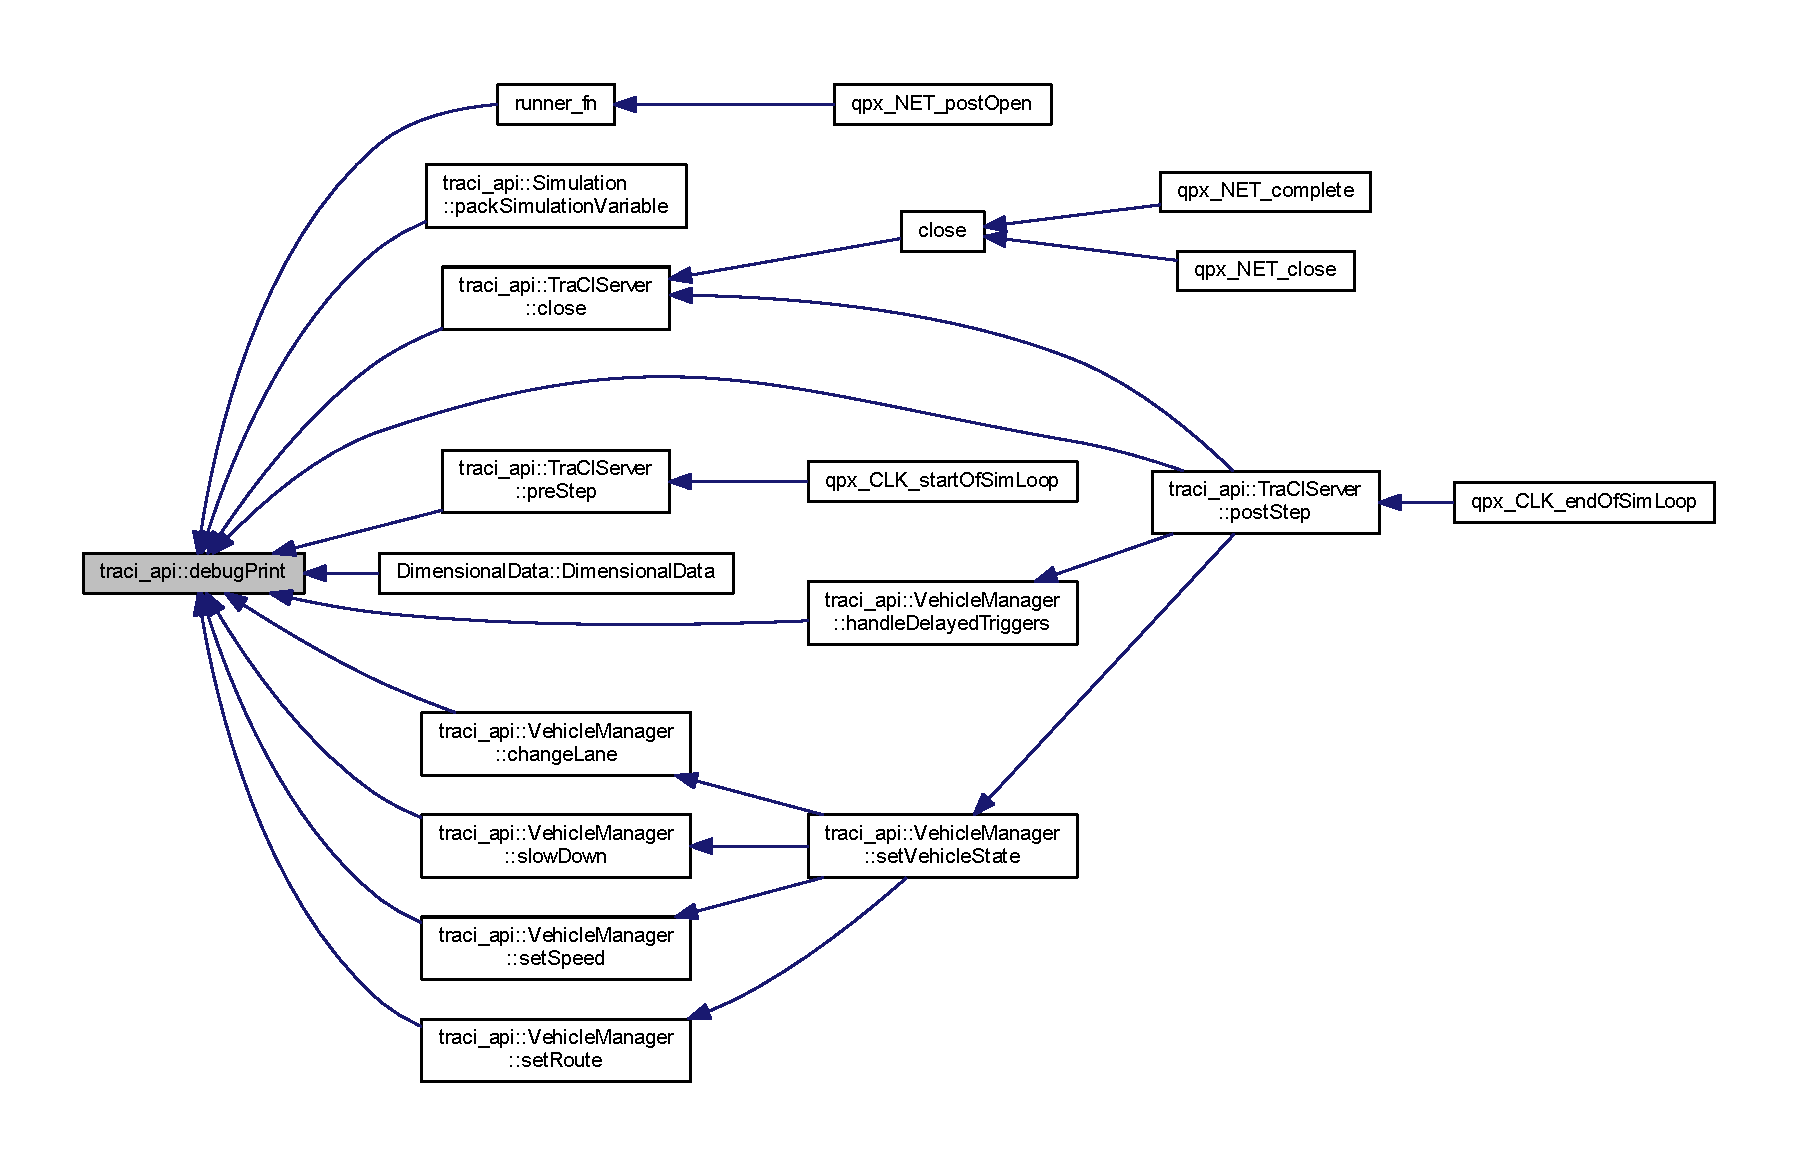
\includegraphics[width=350pt]{namespacetraci__api_a8179b41c12626fc5444d12ee3a6f19cb_icgraph}
\end{center}
\end{figure}
\mbox{\Hypertarget{namespacetraci__api_a3d103fa606d4762c375bac42c66f62a8}\label{namespacetraci__api_a3d103fa606d4762c375bac42c66f62a8}} 
\index{traci\+\_\+api@{traci\+\_\+api}!info\+Print@{info\+Print}}
\index{info\+Print@{info\+Print}!traci\+\_\+api@{traci\+\_\+api}}
\subsubsection{\texorpdfstring{info\+Print()}{infoPrint()}}
{\footnotesize\ttfamily void traci\+\_\+api\+::info\+Print (\begin{DoxyParamCaption}\item[{std\+::string}]{text }\end{DoxyParamCaption})}

Here is the caller graph for this function\+:\nopagebreak
\begin{figure}[H]
\begin{center}
\leavevmode
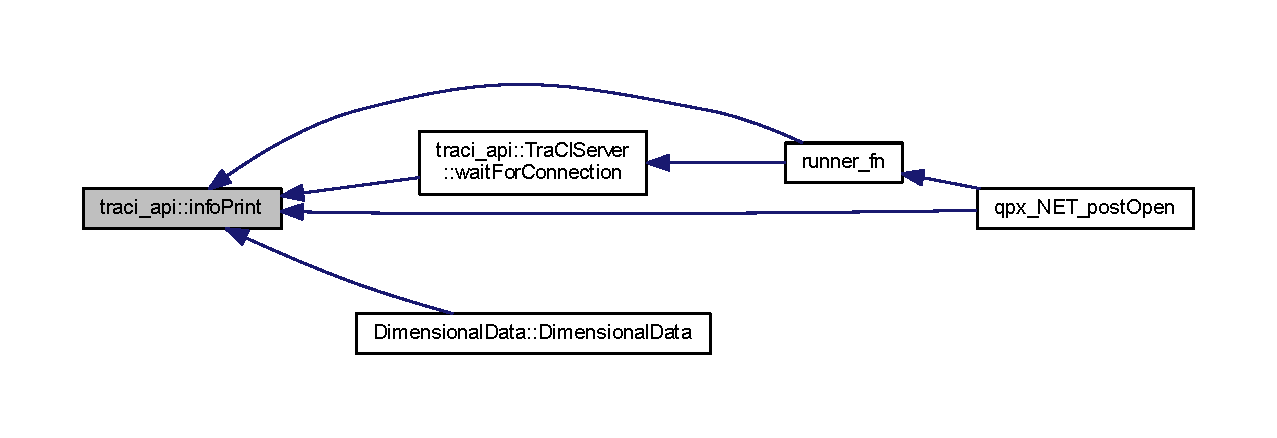
\includegraphics[width=350pt]{namespacetraci__api_a3d103fa606d4762c375bac42c66f62a8_icgraph}
\end{center}
\end{figure}
\mbox{\Hypertarget{namespacetraci__api_aee58441392da7b83ecd8c8831271e945}\label{namespacetraci__api_aee58441392da7b83ecd8c8831271e945}} 
\index{traci\+\_\+api@{traci\+\_\+api}!read\+Type\+Checking\+Byte@{read\+Type\+Checking\+Byte}}
\index{read\+Type\+Checking\+Byte@{read\+Type\+Checking\+Byte}!traci\+\_\+api@{traci\+\_\+api}}
\subsubsection{\texorpdfstring{read\+Type\+Checking\+Byte()}{readTypeCheckingByte()}}
{\footnotesize\ttfamily bool traci\+\_\+api\+::read\+Type\+Checking\+Byte (\begin{DoxyParamCaption}\item[{\hyperlink{classtcpip_1_1_storage}{tcpip\+::\+Storage} \&}]{input\+Storage,  }\item[{int8\+\_\+t \&}]{into }\end{DoxyParamCaption})}



Reads the value type and a 2D bounding box, verifying the type. 


\begin{DoxyParams}{Parameters}
{\em } & \\
\hline
\end{DoxyParams}
Here is the call graph for this function\+:\nopagebreak
\begin{figure}[H]
\begin{center}
\leavevmode
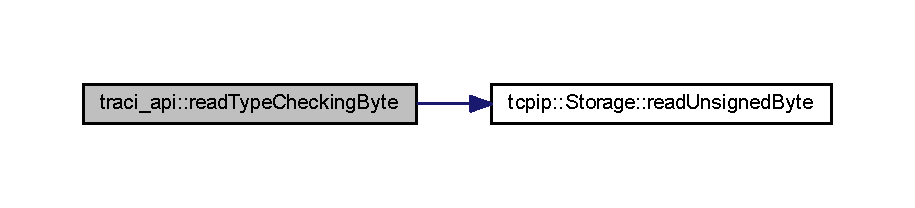
\includegraphics[width=350pt]{namespacetraci__api_aee58441392da7b83ecd8c8831271e945_cgraph}
\end{center}
\end{figure}
Here is the caller graph for this function\+:\nopagebreak
\begin{figure}[H]
\begin{center}
\leavevmode
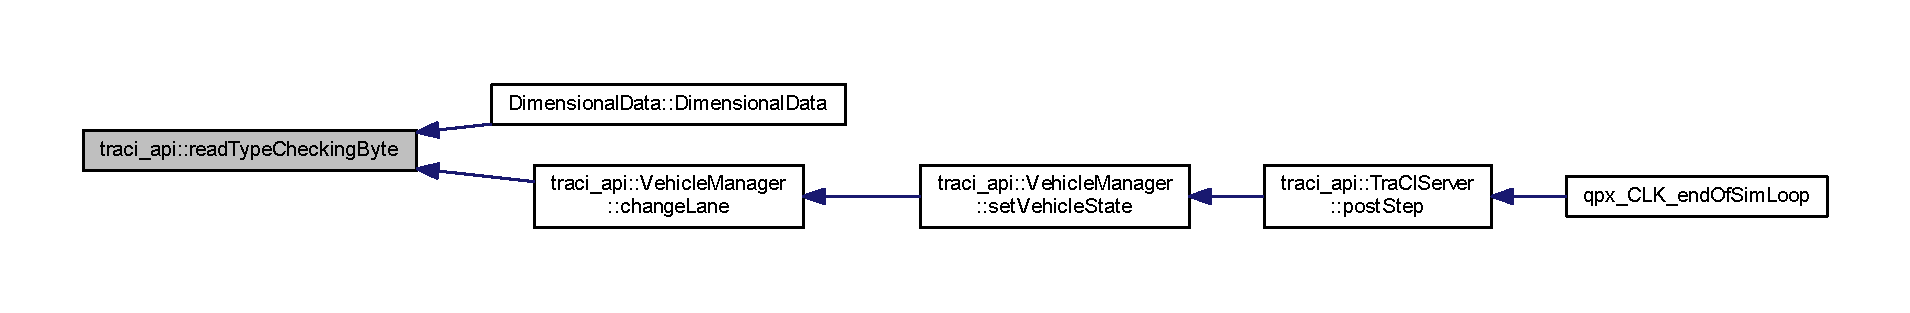
\includegraphics[width=350pt]{namespacetraci__api_aee58441392da7b83ecd8c8831271e945_icgraph}
\end{center}
\end{figure}
\mbox{\Hypertarget{namespacetraci__api_af8c7656fbd212acb13f037d4fb20f1f7}\label{namespacetraci__api_af8c7656fbd212acb13f037d4fb20f1f7}} 
\index{traci\+\_\+api@{traci\+\_\+api}!read\+Type\+Checking\+Color@{read\+Type\+Checking\+Color}}
\index{read\+Type\+Checking\+Color@{read\+Type\+Checking\+Color}!traci\+\_\+api@{traci\+\_\+api}}
\subsubsection{\texorpdfstring{read\+Type\+Checking\+Color()}{readTypeCheckingColor()}}
{\footnotesize\ttfamily bool traci\+\_\+api\+::read\+Type\+Checking\+Color (\begin{DoxyParamCaption}\item[{\hyperlink{classtcpip_1_1_storage}{tcpip\+::\+Storage} \&}]{input\+Storage,  }\item[{uint32\+\_\+t \&}]{hex }\end{DoxyParamCaption})}



Reads the value type and a color, verifying the type. 


\begin{DoxyParams}{Parameters}
{\em } & \\
\hline
\end{DoxyParams}
Here is the call graph for this function\+:\nopagebreak
\begin{figure}[H]
\begin{center}
\leavevmode
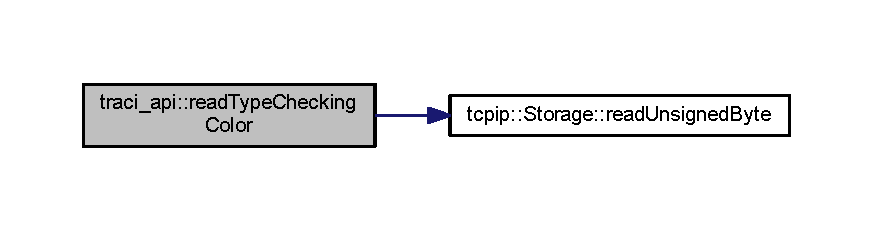
\includegraphics[width=350pt]{namespacetraci__api_af8c7656fbd212acb13f037d4fb20f1f7_cgraph}
\end{center}
\end{figure}
Here is the caller graph for this function\+:\nopagebreak
\begin{figure}[H]
\begin{center}
\leavevmode
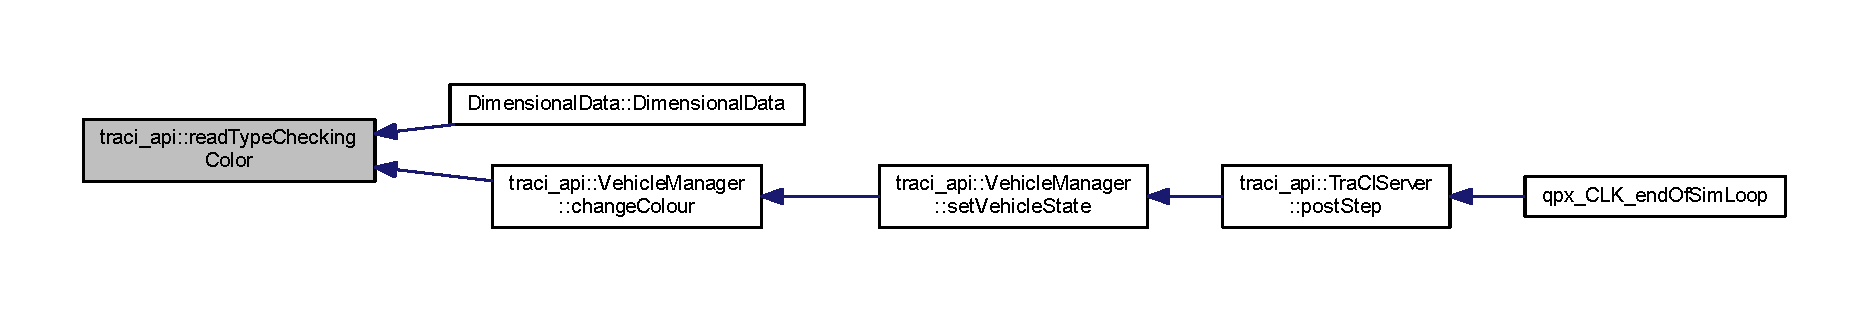
\includegraphics[width=350pt]{namespacetraci__api_af8c7656fbd212acb13f037d4fb20f1f7_icgraph}
\end{center}
\end{figure}
\mbox{\Hypertarget{namespacetraci__api_a5229be0b43fc9f5d9f413d5e51924b50}\label{namespacetraci__api_a5229be0b43fc9f5d9f413d5e51924b50}} 
\index{traci\+\_\+api@{traci\+\_\+api}!read\+Type\+Checking\+Double@{read\+Type\+Checking\+Double}}
\index{read\+Type\+Checking\+Double@{read\+Type\+Checking\+Double}!traci\+\_\+api@{traci\+\_\+api}}
\subsubsection{\texorpdfstring{read\+Type\+Checking\+Double()}{readTypeCheckingDouble()}}
{\footnotesize\ttfamily bool traci\+\_\+api\+::read\+Type\+Checking\+Double (\begin{DoxyParamCaption}\item[{\hyperlink{classtcpip_1_1_storage}{tcpip\+::\+Storage} \&}]{input\+Storage,  }\item[{double \&}]{into }\end{DoxyParamCaption})}



Reads the value type and a double, verifying the type. 


\begin{DoxyParams}{Parameters}
{\em } & \\
\hline
\end{DoxyParams}
Here is the call graph for this function\+:\nopagebreak
\begin{figure}[H]
\begin{center}
\leavevmode
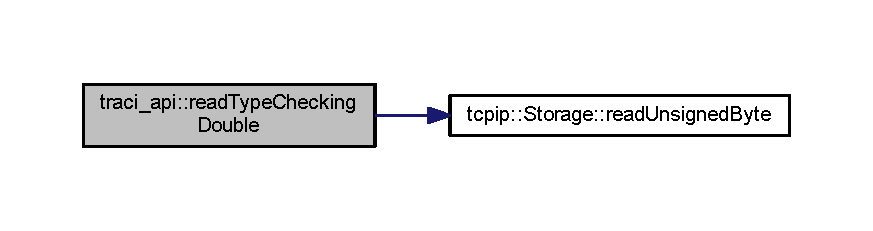
\includegraphics[width=350pt]{namespacetraci__api_a5229be0b43fc9f5d9f413d5e51924b50_cgraph}
\end{center}
\end{figure}
Here is the caller graph for this function\+:\nopagebreak
\begin{figure}[H]
\begin{center}
\leavevmode
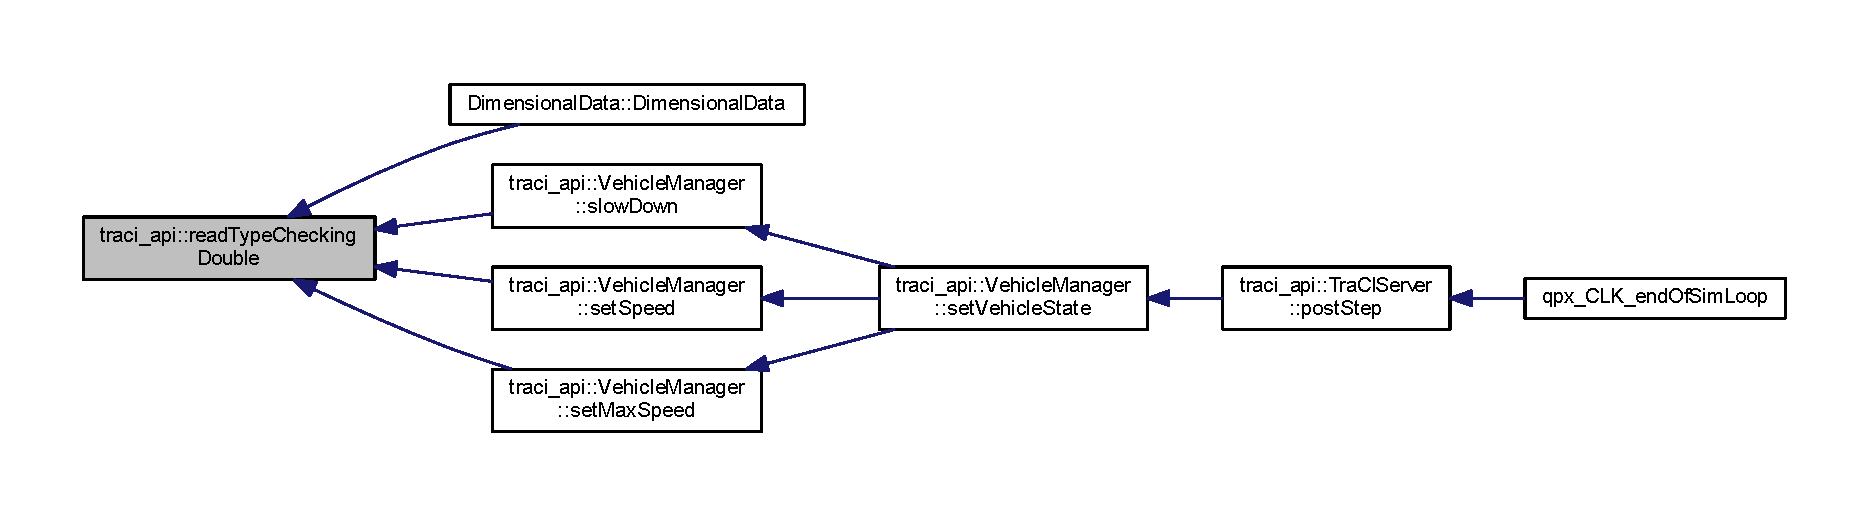
\includegraphics[width=350pt]{namespacetraci__api_a5229be0b43fc9f5d9f413d5e51924b50_icgraph}
\end{center}
\end{figure}
\mbox{\Hypertarget{namespacetraci__api_a57c1a8583619eb1e9984249249435f8e}\label{namespacetraci__api_a57c1a8583619eb1e9984249249435f8e}} 
\index{traci\+\_\+api@{traci\+\_\+api}!read\+Type\+Checking\+Int@{read\+Type\+Checking\+Int}}
\index{read\+Type\+Checking\+Int@{read\+Type\+Checking\+Int}!traci\+\_\+api@{traci\+\_\+api}}
\subsubsection{\texorpdfstring{read\+Type\+Checking\+Int()}{readTypeCheckingInt()}}
{\footnotesize\ttfamily bool traci\+\_\+api\+::read\+Type\+Checking\+Int (\begin{DoxyParamCaption}\item[{\hyperlink{classtcpip_1_1_storage}{tcpip\+::\+Storage} \&}]{input\+Storage,  }\item[{int \&}]{into }\end{DoxyParamCaption})}



Reads the value type and an int, verifying the type. 


\begin{DoxyParams}{Parameters}
{\em } & \\
\hline
\end{DoxyParams}
Here is the call graph for this function\+:\nopagebreak
\begin{figure}[H]
\begin{center}
\leavevmode
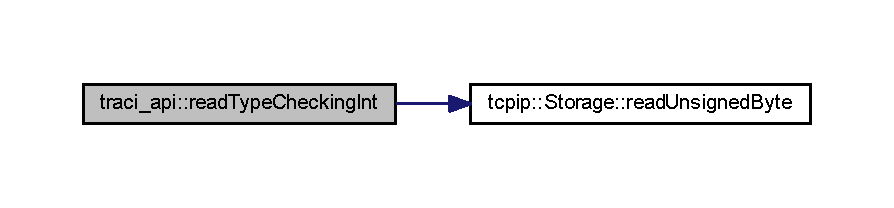
\includegraphics[width=350pt]{namespacetraci__api_a57c1a8583619eb1e9984249249435f8e_cgraph}
\end{center}
\end{figure}
Here is the caller graph for this function\+:\nopagebreak
\begin{figure}[H]
\begin{center}
\leavevmode
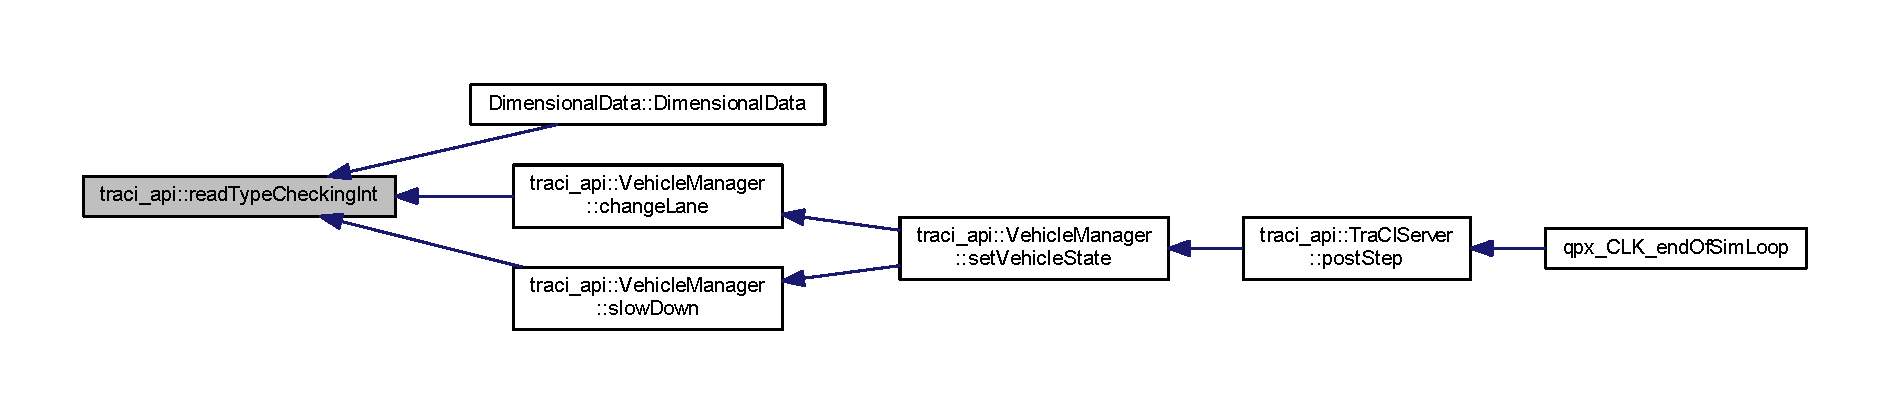
\includegraphics[width=350pt]{namespacetraci__api_a57c1a8583619eb1e9984249249435f8e_icgraph}
\end{center}
\end{figure}
\mbox{\Hypertarget{namespacetraci__api_a26421201e19b2667e198708c2216ca06}\label{namespacetraci__api_a26421201e19b2667e198708c2216ca06}} 
\index{traci\+\_\+api@{traci\+\_\+api}!read\+Type\+Checking\+Position2D@{read\+Type\+Checking\+Position2D}}
\index{read\+Type\+Checking\+Position2D@{read\+Type\+Checking\+Position2D}!traci\+\_\+api@{traci\+\_\+api}}
\subsubsection{\texorpdfstring{read\+Type\+Checking\+Position2\+D()}{readTypeCheckingPosition2D()}}
{\footnotesize\ttfamily bool traci\+\_\+api\+::read\+Type\+Checking\+Position2D (\begin{DoxyParamCaption}\item[{\hyperlink{classtcpip_1_1_storage}{tcpip\+::\+Storage} \&}]{input\+Storage,  }\item[{\hyperlink{class_vector2_d}{Vector2D} \&}]{into }\end{DoxyParamCaption})}



Reads the value type and a 2D position, verifying the type. 


\begin{DoxyParams}{Parameters}
{\em } & \\
\hline
\end{DoxyParams}
Here is the call graph for this function\+:\nopagebreak
\begin{figure}[H]
\begin{center}
\leavevmode
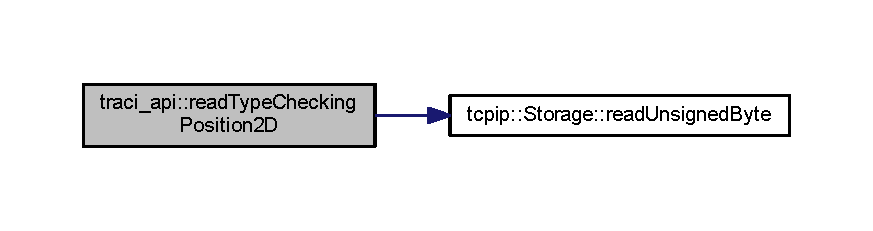
\includegraphics[width=350pt]{namespacetraci__api_a26421201e19b2667e198708c2216ca06_cgraph}
\end{center}
\end{figure}
Here is the caller graph for this function\+:\nopagebreak
\begin{figure}[H]
\begin{center}
\leavevmode
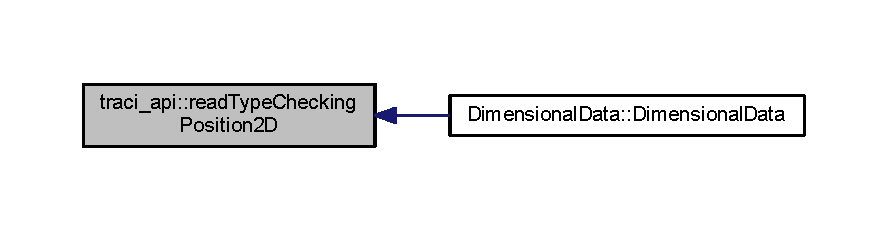
\includegraphics[width=350pt]{namespacetraci__api_a26421201e19b2667e198708c2216ca06_icgraph}
\end{center}
\end{figure}
\mbox{\Hypertarget{namespacetraci__api_ac51a66efdbed4dcdcef596643fe387ec}\label{namespacetraci__api_ac51a66efdbed4dcdcef596643fe387ec}} 
\index{traci\+\_\+api@{traci\+\_\+api}!read\+Type\+Checking\+String@{read\+Type\+Checking\+String}}
\index{read\+Type\+Checking\+String@{read\+Type\+Checking\+String}!traci\+\_\+api@{traci\+\_\+api}}
\subsubsection{\texorpdfstring{read\+Type\+Checking\+String()}{readTypeCheckingString()}}
{\footnotesize\ttfamily bool traci\+\_\+api\+::read\+Type\+Checking\+String (\begin{DoxyParamCaption}\item[{\hyperlink{classtcpip_1_1_storage}{tcpip\+::\+Storage} \&}]{input\+Storage,  }\item[{std\+::string \&}]{into }\end{DoxyParamCaption})}



Reads the value type and a string, verifying the type. 


\begin{DoxyParams}{Parameters}
{\em } & \\
\hline
\end{DoxyParams}
Here is the call graph for this function\+:\nopagebreak
\begin{figure}[H]
\begin{center}
\leavevmode
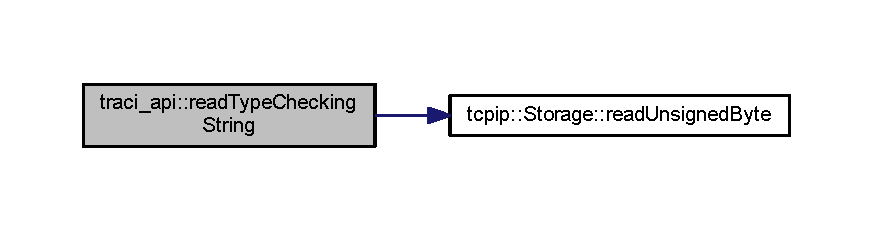
\includegraphics[width=350pt]{namespacetraci__api_ac51a66efdbed4dcdcef596643fe387ec_cgraph}
\end{center}
\end{figure}
Here is the caller graph for this function\+:\nopagebreak
\begin{figure}[H]
\begin{center}
\leavevmode
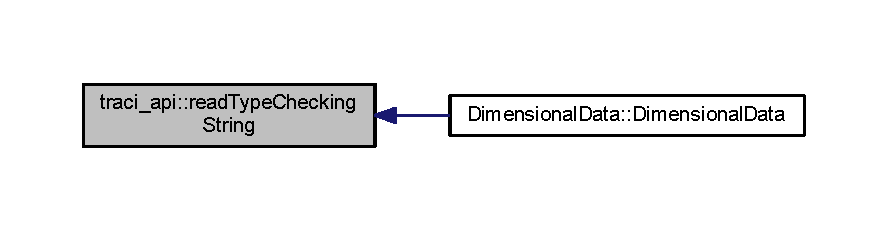
\includegraphics[width=350pt]{namespacetraci__api_ac51a66efdbed4dcdcef596643fe387ec_icgraph}
\end{center}
\end{figure}
\mbox{\Hypertarget{namespacetraci__api_aa16305c07ac5f8221d9099f2e3a7531c}\label{namespacetraci__api_aa16305c07ac5f8221d9099f2e3a7531c}} 
\index{traci\+\_\+api@{traci\+\_\+api}!read\+Type\+Checking\+String\+List@{read\+Type\+Checking\+String\+List}}
\index{read\+Type\+Checking\+String\+List@{read\+Type\+Checking\+String\+List}!traci\+\_\+api@{traci\+\_\+api}}
\subsubsection{\texorpdfstring{read\+Type\+Checking\+String\+List()}{readTypeCheckingStringList()}}
{\footnotesize\ttfamily bool traci\+\_\+api\+::read\+Type\+Checking\+String\+List (\begin{DoxyParamCaption}\item[{\hyperlink{classtcpip_1_1_storage}{tcpip\+::\+Storage} \&}]{input\+Storage,  }\item[{std\+::vector$<$ std\+::string $>$ \&}]{into }\end{DoxyParamCaption})}



Reads the value type and a string list, verifying the type. 


\begin{DoxyParams}{Parameters}
{\em } & \\
\hline
\end{DoxyParams}
Here is the call graph for this function\+:\nopagebreak
\begin{figure}[H]
\begin{center}
\leavevmode
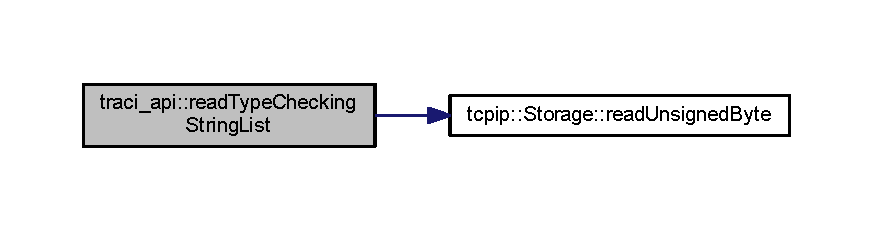
\includegraphics[width=350pt]{namespacetraci__api_aa16305c07ac5f8221d9099f2e3a7531c_cgraph}
\end{center}
\end{figure}
Here is the caller graph for this function\+:\nopagebreak
\begin{figure}[H]
\begin{center}
\leavevmode
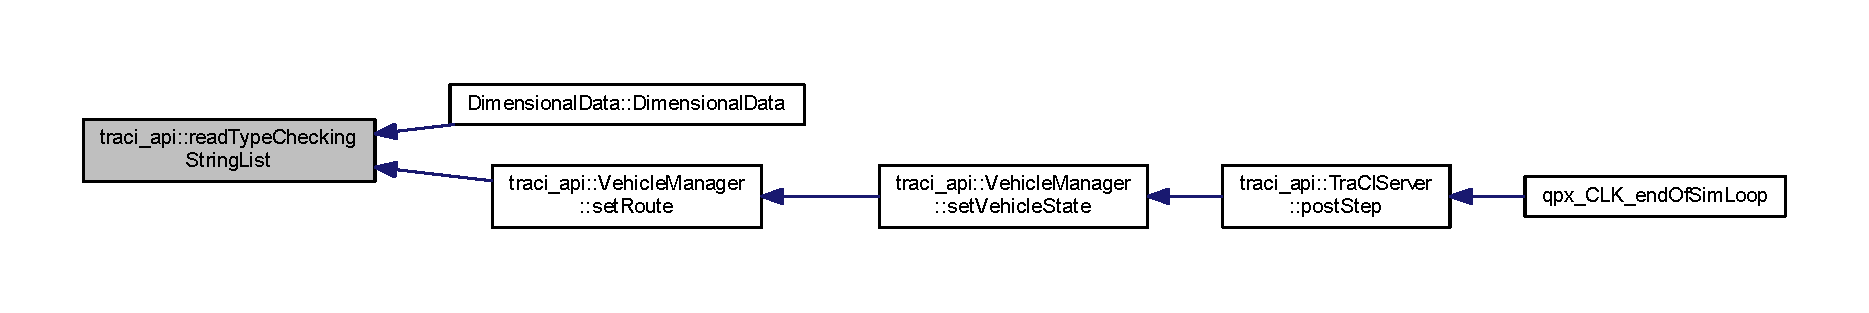
\includegraphics[width=350pt]{namespacetraci__api_aa16305c07ac5f8221d9099f2e3a7531c_icgraph}
\end{center}
\end{figure}
\mbox{\Hypertarget{namespacetraci__api_ac95893093cb3b220faafd74ce62abba3}\label{namespacetraci__api_ac95893093cb3b220faafd74ce62abba3}} 
\index{traci\+\_\+api@{traci\+\_\+api}!read\+Type\+Checking\+Unsigned\+Byte@{read\+Type\+Checking\+Unsigned\+Byte}}
\index{read\+Type\+Checking\+Unsigned\+Byte@{read\+Type\+Checking\+Unsigned\+Byte}!traci\+\_\+api@{traci\+\_\+api}}
\subsubsection{\texorpdfstring{read\+Type\+Checking\+Unsigned\+Byte()}{readTypeCheckingUnsignedByte()}}
{\footnotesize\ttfamily bool traci\+\_\+api\+::read\+Type\+Checking\+Unsigned\+Byte (\begin{DoxyParamCaption}\item[{\hyperlink{classtcpip_1_1_storage}{tcpip\+::\+Storage} \&}]{input\+Storage,  }\item[{uint8\+\_\+t \&}]{into }\end{DoxyParamCaption})}



Reads the value type and an unsigned byte, verifying the type. 


\begin{DoxyParams}{Parameters}
{\em } & \\
\hline
\end{DoxyParams}
Here is the call graph for this function\+:\nopagebreak
\begin{figure}[H]
\begin{center}
\leavevmode
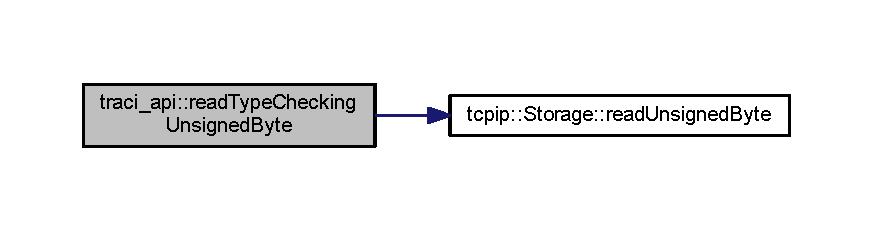
\includegraphics[width=350pt]{namespacetraci__api_ac95893093cb3b220faafd74ce62abba3_cgraph}
\end{center}
\end{figure}
Here is the caller graph for this function\+:\nopagebreak
\begin{figure}[H]
\begin{center}
\leavevmode
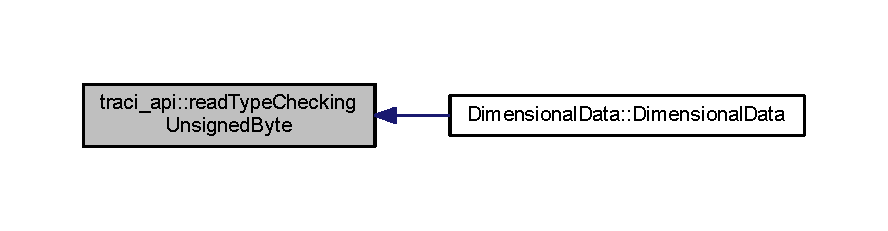
\includegraphics[width=350pt]{namespacetraci__api_ac95893093cb3b220faafd74ce62abba3_icgraph}
\end{center}
\end{figure}

\chapter{Class Documentation}
\hypertarget{classtraci__api_1_1_base_speed_controller}{}\section{traci\+\_\+api\+:\+:Base\+Speed\+Controller Class Reference}
\label{classtraci__api_1_1_base_speed_controller}\index{traci\+\_\+api\+::\+Base\+Speed\+Controller@{traci\+\_\+api\+::\+Base\+Speed\+Controller}}


{\ttfamily \#include $<$Triggers.\+h$>$}



Inheritance diagram for traci\+\_\+api\+:\+:Base\+Speed\+Controller\+:
\nopagebreak
\begin{figure}[H]
\begin{center}
\leavevmode
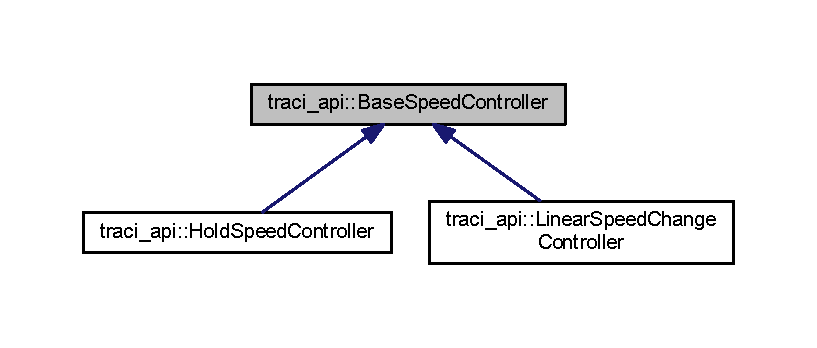
\includegraphics[width=350pt]{classtraci__api_1_1_base_speed_controller__inherit__graph}
\end{center}
\end{figure}
\subsection*{Public Member Functions}
\begin{DoxyCompactItemize}
\item 
virtual \hyperlink{classtraci__api_1_1_base_speed_controller_a7cabfad7b110f2463c62fe9e1d882043}{$\sim$\+Base\+Speed\+Controller} ()
\item 
virtual float \hyperlink{classtraci__api_1_1_base_speed_controller_ab9658ce36f91de8a34bb710b3241c210}{next\+Time\+Step} ()=0
\item 
virtual bool \hyperlink{classtraci__api_1_1_base_speed_controller_a2d4b22945d4cb27f5fe24b05700021b6}{repeat} ()=0
\end{DoxyCompactItemize}


\subsection{Constructor \& Destructor Documentation}
\mbox{\Hypertarget{classtraci__api_1_1_base_speed_controller_a7cabfad7b110f2463c62fe9e1d882043}\label{classtraci__api_1_1_base_speed_controller_a7cabfad7b110f2463c62fe9e1d882043}} 
\index{traci\+\_\+api\+::\+Base\+Speed\+Controller@{traci\+\_\+api\+::\+Base\+Speed\+Controller}!````~Base\+Speed\+Controller@{$\sim$\+Base\+Speed\+Controller}}
\index{````~Base\+Speed\+Controller@{$\sim$\+Base\+Speed\+Controller}!traci\+\_\+api\+::\+Base\+Speed\+Controller@{traci\+\_\+api\+::\+Base\+Speed\+Controller}}
\subsubsection{\texorpdfstring{$\sim$\+Base\+Speed\+Controller()}{~BaseSpeedController()}}
{\footnotesize\ttfamily virtual traci\+\_\+api\+::\+Base\+Speed\+Controller\+::$\sim$\+Base\+Speed\+Controller (\begin{DoxyParamCaption}{ }\end{DoxyParamCaption})\hspace{0.3cm}{\ttfamily [inline]}, {\ttfamily [virtual]}}

Here is the call graph for this function\+:
\nopagebreak
\begin{figure}[H]
\begin{center}
\leavevmode
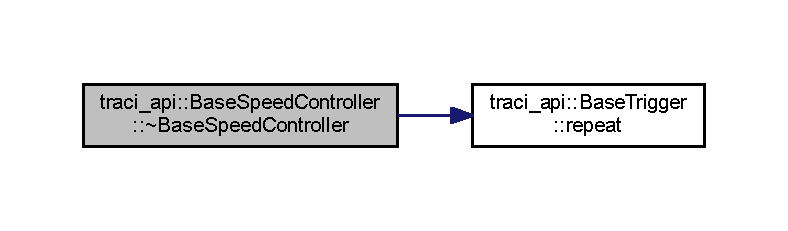
\includegraphics[width=350pt]{classtraci__api_1_1_base_speed_controller_a7cabfad7b110f2463c62fe9e1d882043_cgraph}
\end{center}
\end{figure}


\subsection{Member Function Documentation}
\mbox{\Hypertarget{classtraci__api_1_1_base_speed_controller_ab9658ce36f91de8a34bb710b3241c210}\label{classtraci__api_1_1_base_speed_controller_ab9658ce36f91de8a34bb710b3241c210}} 
\index{traci\+\_\+api\+::\+Base\+Speed\+Controller@{traci\+\_\+api\+::\+Base\+Speed\+Controller}!next\+Time\+Step@{next\+Time\+Step}}
\index{next\+Time\+Step@{next\+Time\+Step}!traci\+\_\+api\+::\+Base\+Speed\+Controller@{traci\+\_\+api\+::\+Base\+Speed\+Controller}}
\subsubsection{\texorpdfstring{next\+Time\+Step()}{nextTimeStep()}}
{\footnotesize\ttfamily virtual float traci\+\_\+api\+::\+Base\+Speed\+Controller\+::next\+Time\+Step (\begin{DoxyParamCaption}{ }\end{DoxyParamCaption})\hspace{0.3cm}{\ttfamily [pure virtual]}}



Implemented in \hyperlink{classtraci__api_1_1_linear_speed_change_controller_a31e52d6f77c96a88dda160226335bacd}{traci\+\_\+api\+::\+Linear\+Speed\+Change\+Controller}, and \hyperlink{classtraci__api_1_1_hold_speed_controller_a61476bf22b8252d2a0badd2214b7357a}{traci\+\_\+api\+::\+Hold\+Speed\+Controller}.

Here is the caller graph for this function\+:
\nopagebreak
\begin{figure}[H]
\begin{center}
\leavevmode
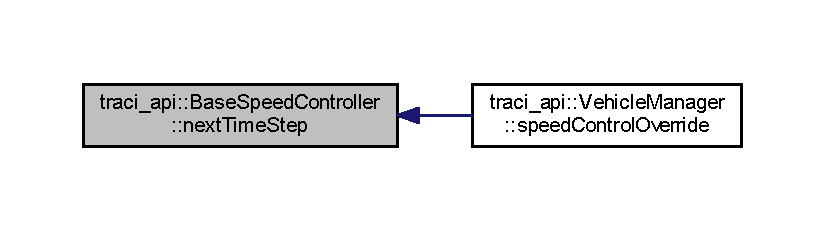
\includegraphics[width=350pt]{classtraci__api_1_1_base_speed_controller_ab9658ce36f91de8a34bb710b3241c210_icgraph}
\end{center}
\end{figure}
\mbox{\Hypertarget{classtraci__api_1_1_base_speed_controller_a2d4b22945d4cb27f5fe24b05700021b6}\label{classtraci__api_1_1_base_speed_controller_a2d4b22945d4cb27f5fe24b05700021b6}} 
\index{traci\+\_\+api\+::\+Base\+Speed\+Controller@{traci\+\_\+api\+::\+Base\+Speed\+Controller}!repeat@{repeat}}
\index{repeat@{repeat}!traci\+\_\+api\+::\+Base\+Speed\+Controller@{traci\+\_\+api\+::\+Base\+Speed\+Controller}}
\subsubsection{\texorpdfstring{repeat()}{repeat()}}
{\footnotesize\ttfamily virtual bool traci\+\_\+api\+::\+Base\+Speed\+Controller\+::repeat (\begin{DoxyParamCaption}{ }\end{DoxyParamCaption})\hspace{0.3cm}{\ttfamily [pure virtual]}}



Implemented in \hyperlink{classtraci__api_1_1_linear_speed_change_controller_aaa5f31ea0c57db838a5786509fc03446}{traci\+\_\+api\+::\+Linear\+Speed\+Change\+Controller}, and \hyperlink{classtraci__api_1_1_hold_speed_controller_acf2f2b8595dd8a135b13be736ee29d63}{traci\+\_\+api\+::\+Hold\+Speed\+Controller}.

Here is the caller graph for this function\+:
\nopagebreak
\begin{figure}[H]
\begin{center}
\leavevmode
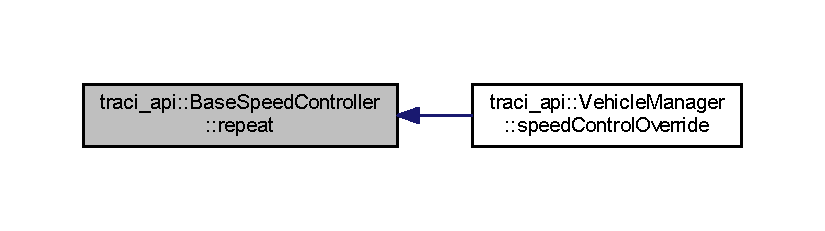
\includegraphics[width=350pt]{classtraci__api_1_1_base_speed_controller_a2d4b22945d4cb27f5fe24b05700021b6_icgraph}
\end{center}
\end{figure}


The documentation for this class was generated from the following file\+:\begin{DoxyCompactItemize}
\item 
C\+:/\+Users/\+Public/paramics/programmer/plugins/pveins/src/\+Tra\+C\+I\+A\+P\+I/\hyperlink{_triggers_8h}{Triggers.\+h}\end{DoxyCompactItemize}

\hypertarget{classtraci__api_1_1_base_trigger}{}\section{traci\+\_\+api\+:\+:Base\+Trigger Class Reference}
\label{classtraci__api_1_1_base_trigger}\index{traci\+\_\+api\+::\+Base\+Trigger@{traci\+\_\+api\+::\+Base\+Trigger}}


{\ttfamily \#include $<$Triggers.\+h$>$}



Inheritance diagram for traci\+\_\+api\+:\+:Base\+Trigger\+:\nopagebreak
\begin{figure}[H]
\begin{center}
\leavevmode
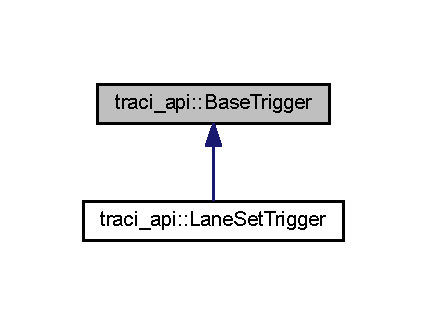
\includegraphics[width=205pt]{classtraci__api_1_1_base_trigger__inherit__graph}
\end{center}
\end{figure}
\subsection*{Public Member Functions}
\begin{DoxyCompactItemize}
\item 
virtual \hyperlink{classtraci__api_1_1_base_trigger_ae1e572064f6b16fa1de9e5416b6c1a9c}{$\sim$\+Base\+Trigger} ()
\item 
virtual void \hyperlink{classtraci__api_1_1_base_trigger_a2de2824fb1d228d4c04aa15c272017a5}{handle\+Trigger} ()=0
\item 
virtual bool \hyperlink{classtraci__api_1_1_base_trigger_a7d2b1ac3f54e42e71eae69f1c7f33943}{repeat} ()=0
\end{DoxyCompactItemize}


\subsection{Constructor \& Destructor Documentation}
\mbox{\Hypertarget{classtraci__api_1_1_base_trigger_ae1e572064f6b16fa1de9e5416b6c1a9c}\label{classtraci__api_1_1_base_trigger_ae1e572064f6b16fa1de9e5416b6c1a9c}} 
\index{traci\+\_\+api\+::\+Base\+Trigger@{traci\+\_\+api\+::\+Base\+Trigger}!````~Base\+Trigger@{$\sim$\+Base\+Trigger}}
\index{````~Base\+Trigger@{$\sim$\+Base\+Trigger}!traci\+\_\+api\+::\+Base\+Trigger@{traci\+\_\+api\+::\+Base\+Trigger}}
\subsubsection{\texorpdfstring{$\sim$\+Base\+Trigger()}{~BaseTrigger()}}
{\footnotesize\ttfamily virtual traci\+\_\+api\+::\+Base\+Trigger\+::$\sim$\+Base\+Trigger (\begin{DoxyParamCaption}{ }\end{DoxyParamCaption})\hspace{0.3cm}{\ttfamily [inline]}, {\ttfamily [virtual]}}

Here is the call graph for this function\+:\nopagebreak
\begin{figure}[H]
\begin{center}
\leavevmode
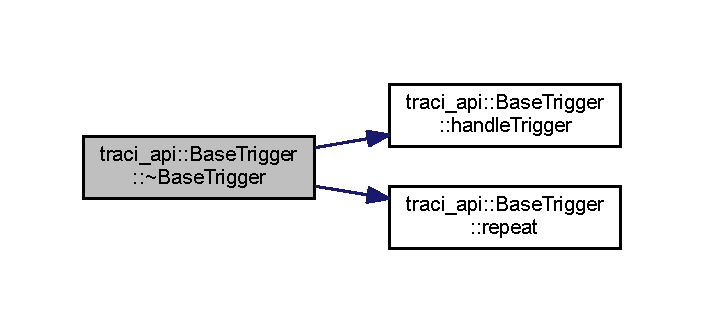
\includegraphics[width=338pt]{classtraci__api_1_1_base_trigger_ae1e572064f6b16fa1de9e5416b6c1a9c_cgraph}
\end{center}
\end{figure}


\subsection{Member Function Documentation}
\mbox{\Hypertarget{classtraci__api_1_1_base_trigger_a2de2824fb1d228d4c04aa15c272017a5}\label{classtraci__api_1_1_base_trigger_a2de2824fb1d228d4c04aa15c272017a5}} 
\index{traci\+\_\+api\+::\+Base\+Trigger@{traci\+\_\+api\+::\+Base\+Trigger}!handle\+Trigger@{handle\+Trigger}}
\index{handle\+Trigger@{handle\+Trigger}!traci\+\_\+api\+::\+Base\+Trigger@{traci\+\_\+api\+::\+Base\+Trigger}}
\subsubsection{\texorpdfstring{handle\+Trigger()}{handleTrigger()}}
{\footnotesize\ttfamily virtual void traci\+\_\+api\+::\+Base\+Trigger\+::handle\+Trigger (\begin{DoxyParamCaption}{ }\end{DoxyParamCaption})\hspace{0.3cm}{\ttfamily [pure virtual]}}



Implemented in \hyperlink{classtraci__api_1_1_lane_set_trigger_a9bc702339daf8aa0d905e3bab5ff2dc3}{traci\+\_\+api\+::\+Lane\+Set\+Trigger}.

Here is the caller graph for this function\+:\nopagebreak
\begin{figure}[H]
\begin{center}
\leavevmode
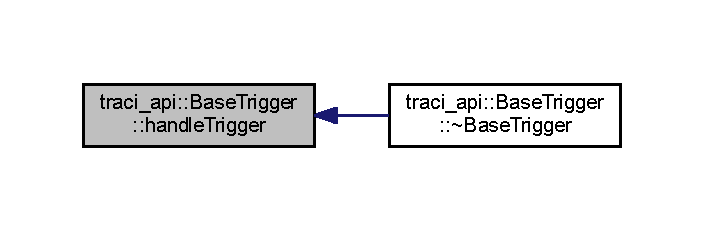
\includegraphics[width=338pt]{classtraci__api_1_1_base_trigger_a2de2824fb1d228d4c04aa15c272017a5_icgraph}
\end{center}
\end{figure}
\mbox{\Hypertarget{classtraci__api_1_1_base_trigger_a7d2b1ac3f54e42e71eae69f1c7f33943}\label{classtraci__api_1_1_base_trigger_a7d2b1ac3f54e42e71eae69f1c7f33943}} 
\index{traci\+\_\+api\+::\+Base\+Trigger@{traci\+\_\+api\+::\+Base\+Trigger}!repeat@{repeat}}
\index{repeat@{repeat}!traci\+\_\+api\+::\+Base\+Trigger@{traci\+\_\+api\+::\+Base\+Trigger}}
\subsubsection{\texorpdfstring{repeat()}{repeat()}}
{\footnotesize\ttfamily virtual bool traci\+\_\+api\+::\+Base\+Trigger\+::repeat (\begin{DoxyParamCaption}{ }\end{DoxyParamCaption})\hspace{0.3cm}{\ttfamily [pure virtual]}}



Implemented in \hyperlink{classtraci__api_1_1_lane_set_trigger_ae606560cb760e12b0f1a86407f614e18}{traci\+\_\+api\+::\+Lane\+Set\+Trigger}.

Here is the caller graph for this function\+:\nopagebreak
\begin{figure}[H]
\begin{center}
\leavevmode
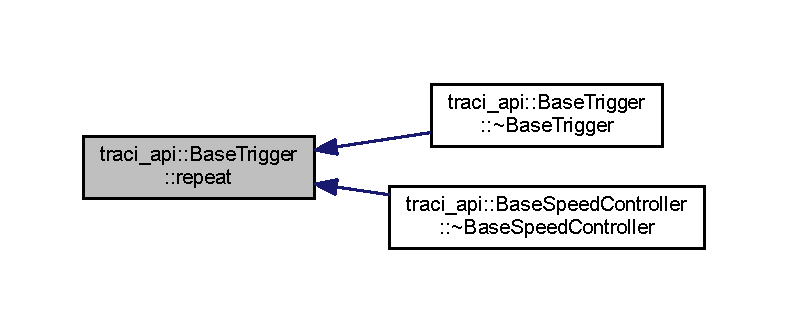
\includegraphics[width=350pt]{classtraci__api_1_1_base_trigger_a7d2b1ac3f54e42e71eae69f1c7f33943_icgraph}
\end{center}
\end{figure}


The documentation for this class was generated from the following file\+:\begin{DoxyCompactItemize}
\item 
C\+:/\+Users/\+Public/paramics/programmer/plugins/pveins/src/\+Tra\+C\+I\+A\+P\+I/\hyperlink{_triggers_8h}{Triggers.\+h}\end{DoxyCompactItemize}

\hypertarget{class_dimensional_data}{}\section{Dimensional\+Data Class Reference}
\label{class_dimensional_data}\index{Dimensional\+Data@{Dimensional\+Data}}


{\ttfamily \#include $<$Utils.\+h$>$}



Collaboration diagram for Dimensional\+Data\+:
\nopagebreak
\begin{figure}[H]
\begin{center}
\leavevmode
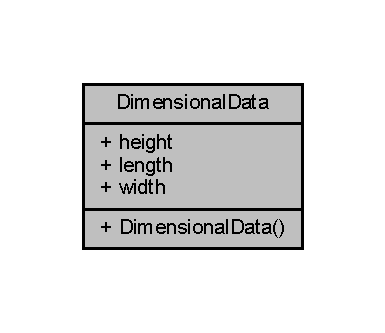
\includegraphics[width=185pt]{class_dimensional_data__coll__graph}
\end{center}
\end{figure}
\subsection*{Public Member Functions}
\begin{DoxyCompactItemize}
\item 
\hyperlink{class_dimensional_data_a85c1d983a7dbe67ed9d93336e37b2b74}{Dimensional\+Data} (double h, double l, double w)
\end{DoxyCompactItemize}
\subsection*{Public Attributes}
\begin{DoxyCompactItemize}
\item 
double \hyperlink{class_dimensional_data_ad5deedd58ab9d79954d33780f0e2fce2}{height}
\item 
double \hyperlink{class_dimensional_data_a07f712bbdabdc7cadc671feb480065a4}{length}
\item 
double \hyperlink{class_dimensional_data_a5ed5474d8c61c0871189f083c76a39f9}{width}
\end{DoxyCompactItemize}


\subsection{Constructor \& Destructor Documentation}
\mbox{\Hypertarget{class_dimensional_data_a85c1d983a7dbe67ed9d93336e37b2b74}\label{class_dimensional_data_a85c1d983a7dbe67ed9d93336e37b2b74}} 
\index{Dimensional\+Data@{Dimensional\+Data}!Dimensional\+Data@{Dimensional\+Data}}
\index{Dimensional\+Data@{Dimensional\+Data}!Dimensional\+Data@{Dimensional\+Data}}
\subsubsection{\texorpdfstring{Dimensional\+Data()}{DimensionalData()}}
{\footnotesize\ttfamily Dimensional\+Data\+::\+Dimensional\+Data (\begin{DoxyParamCaption}\item[{double}]{h,  }\item[{double}]{l,  }\item[{double}]{w }\end{DoxyParamCaption})\hspace{0.3cm}{\ttfamily [inline]}}

Here is the call graph for this function\+:
\nopagebreak
\begin{figure}[H]
\begin{center}
\leavevmode
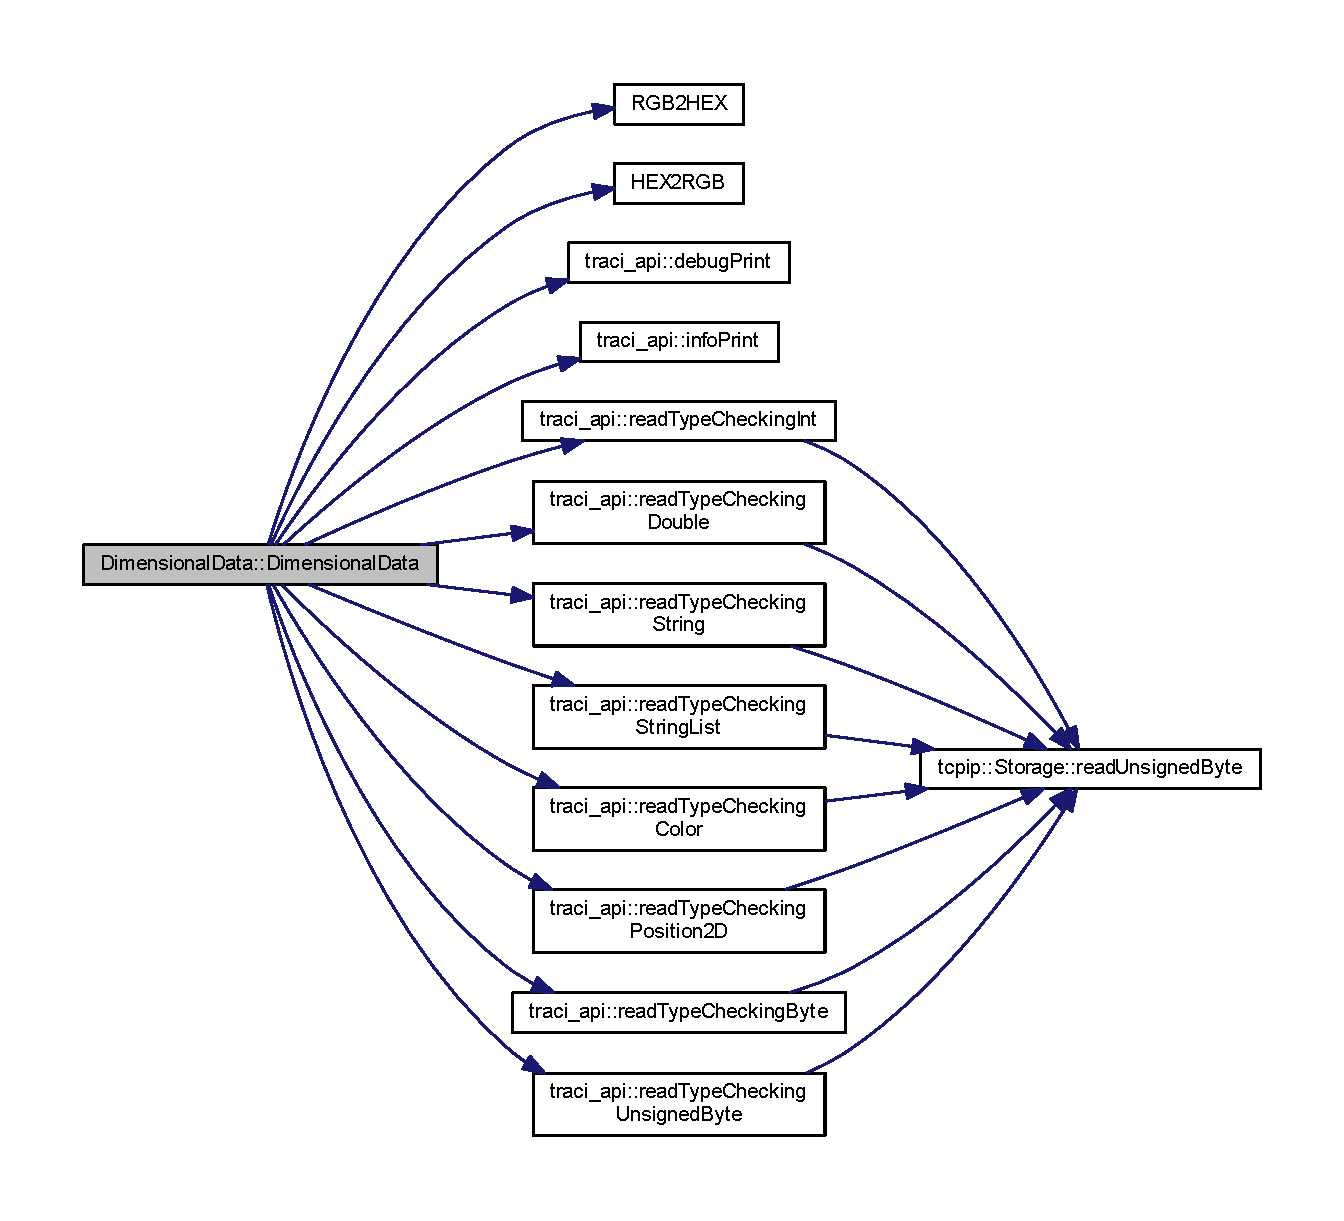
\includegraphics[width=350pt]{class_dimensional_data_a85c1d983a7dbe67ed9d93336e37b2b74_cgraph}
\end{center}
\end{figure}


\subsection{Member Data Documentation}
\mbox{\Hypertarget{class_dimensional_data_ad5deedd58ab9d79954d33780f0e2fce2}\label{class_dimensional_data_ad5deedd58ab9d79954d33780f0e2fce2}} 
\index{Dimensional\+Data@{Dimensional\+Data}!height@{height}}
\index{height@{height}!Dimensional\+Data@{Dimensional\+Data}}
\subsubsection{\texorpdfstring{height}{height}}
{\footnotesize\ttfamily double Dimensional\+Data\+::height}

\mbox{\Hypertarget{class_dimensional_data_a07f712bbdabdc7cadc671feb480065a4}\label{class_dimensional_data_a07f712bbdabdc7cadc671feb480065a4}} 
\index{Dimensional\+Data@{Dimensional\+Data}!length@{length}}
\index{length@{length}!Dimensional\+Data@{Dimensional\+Data}}
\subsubsection{\texorpdfstring{length}{length}}
{\footnotesize\ttfamily double Dimensional\+Data\+::length}

\mbox{\Hypertarget{class_dimensional_data_a5ed5474d8c61c0871189f083c76a39f9}\label{class_dimensional_data_a5ed5474d8c61c0871189f083c76a39f9}} 
\index{Dimensional\+Data@{Dimensional\+Data}!width@{width}}
\index{width@{width}!Dimensional\+Data@{Dimensional\+Data}}
\subsubsection{\texorpdfstring{width}{width}}
{\footnotesize\ttfamily double Dimensional\+Data\+::width}



The documentation for this class was generated from the following file\+:\begin{DoxyCompactItemize}
\item 
C\+:/\+Users/\+Public/paramics/programmer/plugins/pveins/src/\+Tra\+C\+I\+A\+P\+I/\hyperlink{_utils_8h}{Utils.\+h}\end{DoxyCompactItemize}

\hypertarget{classtraci__api_1_1_hold_speed_controller}{}\section{traci\+\_\+api\+:\+:Hold\+Speed\+Controller Class Reference}
\label{classtraci__api_1_1_hold_speed_controller}\index{traci\+\_\+api\+::\+Hold\+Speed\+Controller@{traci\+\_\+api\+::\+Hold\+Speed\+Controller}}


{\ttfamily \#include $<$Triggers.\+h$>$}



Inheritance diagram for traci\+\_\+api\+:\+:Hold\+Speed\+Controller\+:
\nopagebreak
\begin{figure}[H]
\begin{center}
\leavevmode
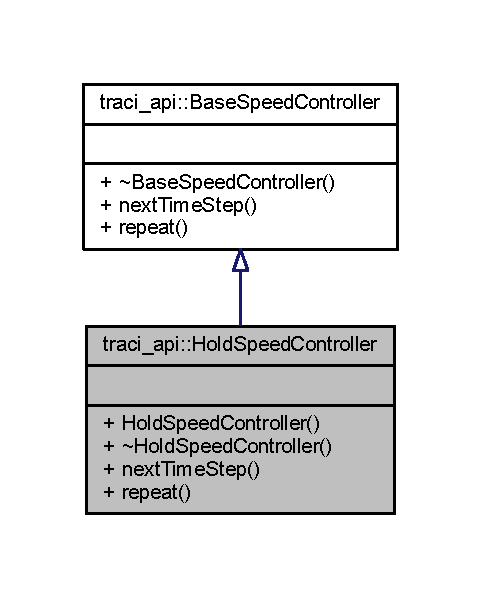
\includegraphics[width=231pt]{classtraci__api_1_1_hold_speed_controller__inherit__graph}
\end{center}
\end{figure}


Collaboration diagram for traci\+\_\+api\+:\+:Hold\+Speed\+Controller\+:
\nopagebreak
\begin{figure}[H]
\begin{center}
\leavevmode
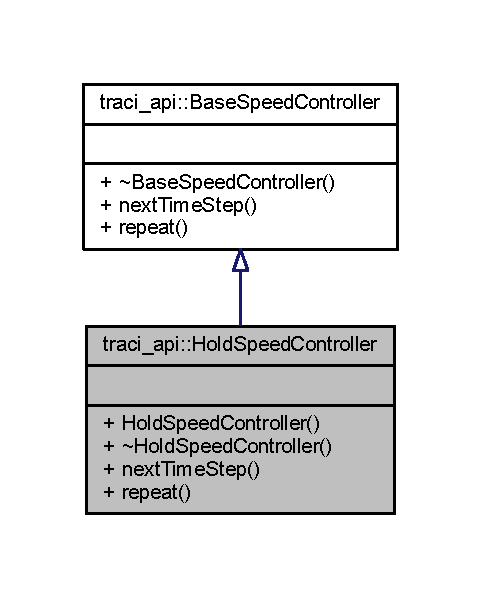
\includegraphics[width=231pt]{classtraci__api_1_1_hold_speed_controller__coll__graph}
\end{center}
\end{figure}
\subsection*{Public Member Functions}
\begin{DoxyCompactItemize}
\item 
\hyperlink{classtraci__api_1_1_hold_speed_controller_a6f55b4ce8db084f9e279635cd56739a4}{Hold\+Speed\+Controller} (V\+E\+H\+I\+C\+LE $\ast$vhc, float target\+\_\+speed)
\item 
\hyperlink{classtraci__api_1_1_hold_speed_controller_a6e9fe04ec1ae839db1ebf2964923781c}{$\sim$\+Hold\+Speed\+Controller} () override
\item 
float \hyperlink{classtraci__api_1_1_hold_speed_controller_a61476bf22b8252d2a0badd2214b7357a}{next\+Time\+Step} () override
\item 
bool \hyperlink{classtraci__api_1_1_hold_speed_controller_acf2f2b8595dd8a135b13be736ee29d63}{repeat} () override
\end{DoxyCompactItemize}


\subsection{Constructor \& Destructor Documentation}
\mbox{\Hypertarget{classtraci__api_1_1_hold_speed_controller_a6f55b4ce8db084f9e279635cd56739a4}\label{classtraci__api_1_1_hold_speed_controller_a6f55b4ce8db084f9e279635cd56739a4}} 
\index{traci\+\_\+api\+::\+Hold\+Speed\+Controller@{traci\+\_\+api\+::\+Hold\+Speed\+Controller}!Hold\+Speed\+Controller@{Hold\+Speed\+Controller}}
\index{Hold\+Speed\+Controller@{Hold\+Speed\+Controller}!traci\+\_\+api\+::\+Hold\+Speed\+Controller@{traci\+\_\+api\+::\+Hold\+Speed\+Controller}}
\subsubsection{\texorpdfstring{Hold\+Speed\+Controller()}{HoldSpeedController()}}
{\footnotesize\ttfamily traci\+\_\+api\+::\+Hold\+Speed\+Controller\+::\+Hold\+Speed\+Controller (\begin{DoxyParamCaption}\item[{V\+E\+H\+I\+C\+LE $\ast$}]{vhc,  }\item[{float}]{target\+\_\+speed }\end{DoxyParamCaption})\hspace{0.3cm}{\ttfamily [inline]}}

\mbox{\Hypertarget{classtraci__api_1_1_hold_speed_controller_a6e9fe04ec1ae839db1ebf2964923781c}\label{classtraci__api_1_1_hold_speed_controller_a6e9fe04ec1ae839db1ebf2964923781c}} 
\index{traci\+\_\+api\+::\+Hold\+Speed\+Controller@{traci\+\_\+api\+::\+Hold\+Speed\+Controller}!````~Hold\+Speed\+Controller@{$\sim$\+Hold\+Speed\+Controller}}
\index{````~Hold\+Speed\+Controller@{$\sim$\+Hold\+Speed\+Controller}!traci\+\_\+api\+::\+Hold\+Speed\+Controller@{traci\+\_\+api\+::\+Hold\+Speed\+Controller}}
\subsubsection{\texorpdfstring{$\sim$\+Hold\+Speed\+Controller()}{~HoldSpeedController()}}
{\footnotesize\ttfamily traci\+\_\+api\+::\+Hold\+Speed\+Controller\+::$\sim$\+Hold\+Speed\+Controller (\begin{DoxyParamCaption}{ }\end{DoxyParamCaption})\hspace{0.3cm}{\ttfamily [inline]}, {\ttfamily [override]}}



\subsection{Member Function Documentation}
\mbox{\Hypertarget{classtraci__api_1_1_hold_speed_controller_a61476bf22b8252d2a0badd2214b7357a}\label{classtraci__api_1_1_hold_speed_controller_a61476bf22b8252d2a0badd2214b7357a}} 
\index{traci\+\_\+api\+::\+Hold\+Speed\+Controller@{traci\+\_\+api\+::\+Hold\+Speed\+Controller}!next\+Time\+Step@{next\+Time\+Step}}
\index{next\+Time\+Step@{next\+Time\+Step}!traci\+\_\+api\+::\+Hold\+Speed\+Controller@{traci\+\_\+api\+::\+Hold\+Speed\+Controller}}
\subsubsection{\texorpdfstring{next\+Time\+Step()}{nextTimeStep()}}
{\footnotesize\ttfamily float traci\+\_\+api\+::\+Hold\+Speed\+Controller\+::next\+Time\+Step (\begin{DoxyParamCaption}{ }\end{DoxyParamCaption})\hspace{0.3cm}{\ttfamily [override]}, {\ttfamily [virtual]}}



Implements \hyperlink{classtraci__api_1_1_base_speed_controller_ab9658ce36f91de8a34bb710b3241c210}{traci\+\_\+api\+::\+Base\+Speed\+Controller}.

\mbox{\Hypertarget{classtraci__api_1_1_hold_speed_controller_acf2f2b8595dd8a135b13be736ee29d63}\label{classtraci__api_1_1_hold_speed_controller_acf2f2b8595dd8a135b13be736ee29d63}} 
\index{traci\+\_\+api\+::\+Hold\+Speed\+Controller@{traci\+\_\+api\+::\+Hold\+Speed\+Controller}!repeat@{repeat}}
\index{repeat@{repeat}!traci\+\_\+api\+::\+Hold\+Speed\+Controller@{traci\+\_\+api\+::\+Hold\+Speed\+Controller}}
\subsubsection{\texorpdfstring{repeat()}{repeat()}}
{\footnotesize\ttfamily bool traci\+\_\+api\+::\+Hold\+Speed\+Controller\+::repeat (\begin{DoxyParamCaption}{ }\end{DoxyParamCaption})\hspace{0.3cm}{\ttfamily [inline]}, {\ttfamily [override]}, {\ttfamily [virtual]}}



Implements \hyperlink{classtraci__api_1_1_base_speed_controller_a2d4b22945d4cb27f5fe24b05700021b6}{traci\+\_\+api\+::\+Base\+Speed\+Controller}.



The documentation for this class was generated from the following files\+:\begin{DoxyCompactItemize}
\item 
C\+:/\+Users/\+Public/paramics/programmer/plugins/pveins/src/\+Tra\+C\+I\+A\+P\+I/\hyperlink{_triggers_8h}{Triggers.\+h}\item 
C\+:/\+Users/\+Public/paramics/programmer/plugins/pveins/src/\+Tra\+C\+I\+A\+P\+I/\hyperlink{_triggers_8cpp}{Triggers.\+cpp}\end{DoxyCompactItemize}

\hypertarget{classtraci__api_1_1_lane_set_trigger}{}\section{traci\+\_\+api\+:\+:Lane\+Set\+Trigger Class Reference}
\label{classtraci__api_1_1_lane_set_trigger}\index{traci\+\_\+api\+::\+Lane\+Set\+Trigger@{traci\+\_\+api\+::\+Lane\+Set\+Trigger}}


{\ttfamily \#include $<$Triggers.\+h$>$}



Inheritance diagram for traci\+\_\+api\+:\+:Lane\+Set\+Trigger\+:\nopagebreak
\begin{figure}[H]
\begin{center}
\leavevmode
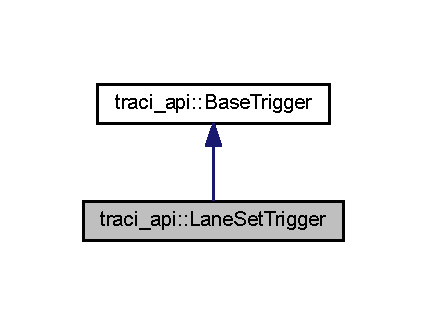
\includegraphics[width=205pt]{classtraci__api_1_1_lane_set_trigger__inherit__graph}
\end{center}
\end{figure}


Collaboration diagram for traci\+\_\+api\+:\+:Lane\+Set\+Trigger\+:\nopagebreak
\begin{figure}[H]
\begin{center}
\leavevmode
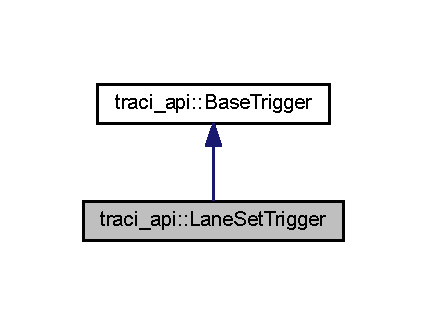
\includegraphics[width=205pt]{classtraci__api_1_1_lane_set_trigger__coll__graph}
\end{center}
\end{figure}
\subsection*{Public Member Functions}
\begin{DoxyCompactItemize}
\item 
\hyperlink{classtraci__api_1_1_lane_set_trigger_a2af85a3a539f5a6c0624085c90cd6fa8}{Lane\+Set\+Trigger} (V\+E\+H\+I\+C\+LE $\ast$vhc, int \hyperlink{classtraci__api_1_1_lane_set_trigger_ad39b2db18176f0a7d40da0bb3878e519}{target\+\_\+lane}, int duration)
\item 
void \hyperlink{classtraci__api_1_1_lane_set_trigger_a9bc702339daf8aa0d905e3bab5ff2dc3}{handle\+Trigger} () override
\item 
bool \hyperlink{classtraci__api_1_1_lane_set_trigger_ae606560cb760e12b0f1a86407f614e18}{repeat} () override
\end{DoxyCompactItemize}
\subsection*{Public Attributes}
\begin{DoxyCompactItemize}
\item 
int \hyperlink{classtraci__api_1_1_lane_set_trigger_ad39b2db18176f0a7d40da0bb3878e519}{target\+\_\+lane}
\item 
int \hyperlink{classtraci__api_1_1_lane_set_trigger_a20d2e675f6c1d69246daa42eeac0153c}{end\+\_\+time}
\item 
V\+E\+H\+I\+C\+LE $\ast$ \hyperlink{classtraci__api_1_1_lane_set_trigger_aec89039cf41fe086fc46c5748e9b933b}{vehicle}
\end{DoxyCompactItemize}


\subsection{Constructor \& Destructor Documentation}
\mbox{\Hypertarget{classtraci__api_1_1_lane_set_trigger_a2af85a3a539f5a6c0624085c90cd6fa8}\label{classtraci__api_1_1_lane_set_trigger_a2af85a3a539f5a6c0624085c90cd6fa8}} 
\index{traci\+\_\+api\+::\+Lane\+Set\+Trigger@{traci\+\_\+api\+::\+Lane\+Set\+Trigger}!Lane\+Set\+Trigger@{Lane\+Set\+Trigger}}
\index{Lane\+Set\+Trigger@{Lane\+Set\+Trigger}!traci\+\_\+api\+::\+Lane\+Set\+Trigger@{traci\+\_\+api\+::\+Lane\+Set\+Trigger}}
\subsubsection{\texorpdfstring{Lane\+Set\+Trigger()}{LaneSetTrigger()}}
{\footnotesize\ttfamily traci\+\_\+api\+::\+Lane\+Set\+Trigger\+::\+Lane\+Set\+Trigger (\begin{DoxyParamCaption}\item[{V\+E\+H\+I\+C\+LE $\ast$}]{vhc,  }\item[{int}]{target\+\_\+lane,  }\item[{int}]{duration }\end{DoxyParamCaption})}

Here is the call graph for this function\+:\nopagebreak
\begin{figure}[H]
\begin{center}
\leavevmode
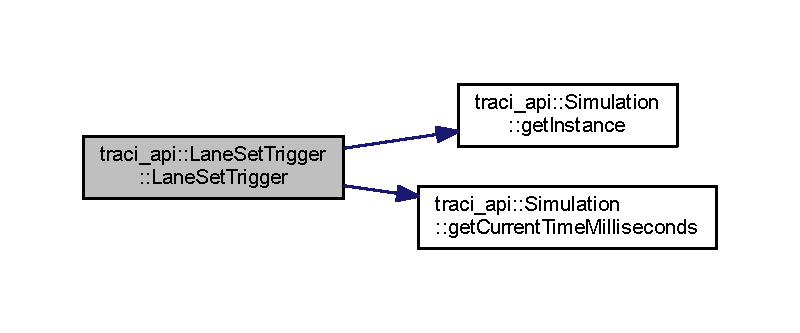
\includegraphics[width=350pt]{classtraci__api_1_1_lane_set_trigger_a2af85a3a539f5a6c0624085c90cd6fa8_cgraph}
\end{center}
\end{figure}


\subsection{Member Function Documentation}
\mbox{\Hypertarget{classtraci__api_1_1_lane_set_trigger_a9bc702339daf8aa0d905e3bab5ff2dc3}\label{classtraci__api_1_1_lane_set_trigger_a9bc702339daf8aa0d905e3bab5ff2dc3}} 
\index{traci\+\_\+api\+::\+Lane\+Set\+Trigger@{traci\+\_\+api\+::\+Lane\+Set\+Trigger}!handle\+Trigger@{handle\+Trigger}}
\index{handle\+Trigger@{handle\+Trigger}!traci\+\_\+api\+::\+Lane\+Set\+Trigger@{traci\+\_\+api\+::\+Lane\+Set\+Trigger}}
\subsubsection{\texorpdfstring{handle\+Trigger()}{handleTrigger()}}
{\footnotesize\ttfamily void traci\+\_\+api\+::\+Lane\+Set\+Trigger\+::handle\+Trigger (\begin{DoxyParamCaption}{ }\end{DoxyParamCaption})\hspace{0.3cm}{\ttfamily [override]}, {\ttfamily [virtual]}}



Implements \hyperlink{classtraci__api_1_1_base_trigger_a2de2824fb1d228d4c04aa15c272017a5}{traci\+\_\+api\+::\+Base\+Trigger}.

\mbox{\Hypertarget{classtraci__api_1_1_lane_set_trigger_ae606560cb760e12b0f1a86407f614e18}\label{classtraci__api_1_1_lane_set_trigger_ae606560cb760e12b0f1a86407f614e18}} 
\index{traci\+\_\+api\+::\+Lane\+Set\+Trigger@{traci\+\_\+api\+::\+Lane\+Set\+Trigger}!repeat@{repeat}}
\index{repeat@{repeat}!traci\+\_\+api\+::\+Lane\+Set\+Trigger@{traci\+\_\+api\+::\+Lane\+Set\+Trigger}}
\subsubsection{\texorpdfstring{repeat()}{repeat()}}
{\footnotesize\ttfamily bool traci\+\_\+api\+::\+Lane\+Set\+Trigger\+::repeat (\begin{DoxyParamCaption}{ }\end{DoxyParamCaption})\hspace{0.3cm}{\ttfamily [override]}, {\ttfamily [virtual]}}



Implements \hyperlink{classtraci__api_1_1_base_trigger_a7d2b1ac3f54e42e71eae69f1c7f33943}{traci\+\_\+api\+::\+Base\+Trigger}.

Here is the call graph for this function\+:\nopagebreak
\begin{figure}[H]
\begin{center}
\leavevmode
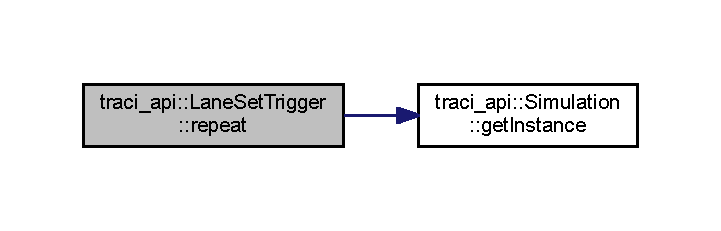
\includegraphics[width=346pt]{classtraci__api_1_1_lane_set_trigger_ae606560cb760e12b0f1a86407f614e18_cgraph}
\end{center}
\end{figure}


\subsection{Member Data Documentation}
\mbox{\Hypertarget{classtraci__api_1_1_lane_set_trigger_a20d2e675f6c1d69246daa42eeac0153c}\label{classtraci__api_1_1_lane_set_trigger_a20d2e675f6c1d69246daa42eeac0153c}} 
\index{traci\+\_\+api\+::\+Lane\+Set\+Trigger@{traci\+\_\+api\+::\+Lane\+Set\+Trigger}!end\+\_\+time@{end\+\_\+time}}
\index{end\+\_\+time@{end\+\_\+time}!traci\+\_\+api\+::\+Lane\+Set\+Trigger@{traci\+\_\+api\+::\+Lane\+Set\+Trigger}}
\subsubsection{\texorpdfstring{end\+\_\+time}{end\_time}}
{\footnotesize\ttfamily int traci\+\_\+api\+::\+Lane\+Set\+Trigger\+::end\+\_\+time}

\mbox{\Hypertarget{classtraci__api_1_1_lane_set_trigger_ad39b2db18176f0a7d40da0bb3878e519}\label{classtraci__api_1_1_lane_set_trigger_ad39b2db18176f0a7d40da0bb3878e519}} 
\index{traci\+\_\+api\+::\+Lane\+Set\+Trigger@{traci\+\_\+api\+::\+Lane\+Set\+Trigger}!target\+\_\+lane@{target\+\_\+lane}}
\index{target\+\_\+lane@{target\+\_\+lane}!traci\+\_\+api\+::\+Lane\+Set\+Trigger@{traci\+\_\+api\+::\+Lane\+Set\+Trigger}}
\subsubsection{\texorpdfstring{target\+\_\+lane}{target\_lane}}
{\footnotesize\ttfamily int traci\+\_\+api\+::\+Lane\+Set\+Trigger\+::target\+\_\+lane}

\mbox{\Hypertarget{classtraci__api_1_1_lane_set_trigger_aec89039cf41fe086fc46c5748e9b933b}\label{classtraci__api_1_1_lane_set_trigger_aec89039cf41fe086fc46c5748e9b933b}} 
\index{traci\+\_\+api\+::\+Lane\+Set\+Trigger@{traci\+\_\+api\+::\+Lane\+Set\+Trigger}!vehicle@{vehicle}}
\index{vehicle@{vehicle}!traci\+\_\+api\+::\+Lane\+Set\+Trigger@{traci\+\_\+api\+::\+Lane\+Set\+Trigger}}
\subsubsection{\texorpdfstring{vehicle}{vehicle}}
{\footnotesize\ttfamily V\+E\+H\+I\+C\+LE$\ast$ traci\+\_\+api\+::\+Lane\+Set\+Trigger\+::vehicle}



The documentation for this class was generated from the following files\+:\begin{DoxyCompactItemize}
\item 
C\+:/\+Users/\+Public/paramics/programmer/plugins/pveins/src/\+Tra\+C\+I\+A\+P\+I/\hyperlink{_triggers_8h}{Triggers.\+h}\item 
C\+:/\+Users/\+Public/paramics/programmer/plugins/pveins/src/\+Tra\+C\+I\+A\+P\+I/\hyperlink{_triggers_8cpp}{Triggers.\+cpp}\end{DoxyCompactItemize}

\hypertarget{classtraci__api_1_1_linear_speed_change_controller}{}\section{traci\+\_\+api\+:\+:Linear\+Speed\+Change\+Controller Class Reference}
\label{classtraci__api_1_1_linear_speed_change_controller}\index{traci\+\_\+api\+::\+Linear\+Speed\+Change\+Controller@{traci\+\_\+api\+::\+Linear\+Speed\+Change\+Controller}}


{\ttfamily \#include $<$Triggers.\+h$>$}



Inheritance diagram for traci\+\_\+api\+:\+:Linear\+Speed\+Change\+Controller\+:
\nopagebreak
\begin{figure}[H]
\begin{center}
\leavevmode
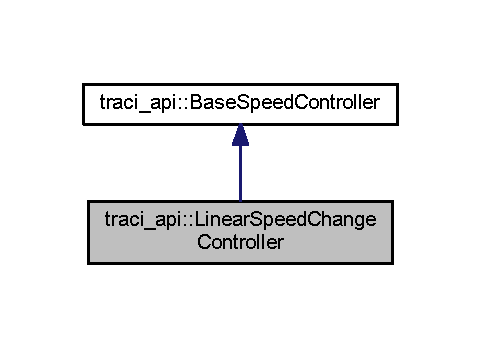
\includegraphics[width=246pt]{classtraci__api_1_1_linear_speed_change_controller__inherit__graph}
\end{center}
\end{figure}


Collaboration diagram for traci\+\_\+api\+:\+:Linear\+Speed\+Change\+Controller\+:
\nopagebreak
\begin{figure}[H]
\begin{center}
\leavevmode
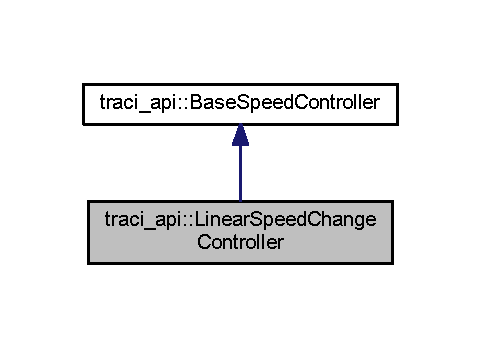
\includegraphics[width=246pt]{classtraci__api_1_1_linear_speed_change_controller__coll__graph}
\end{center}
\end{figure}
\subsection*{Public Member Functions}
\begin{DoxyCompactItemize}
\item 
\hyperlink{classtraci__api_1_1_linear_speed_change_controller_a60f7ef2214d9cd72e7393293c234afa5}{Linear\+Speed\+Change\+Controller} (V\+E\+H\+I\+C\+LE $\ast$vhc, float target\+\_\+speed, int duration)
\item 
\hyperlink{classtraci__api_1_1_linear_speed_change_controller_abb54e5cb6b7befd773ce9bf28df1779f}{$\sim$\+Linear\+Speed\+Change\+Controller} () override
\item 
float \hyperlink{classtraci__api_1_1_linear_speed_change_controller_a31e52d6f77c96a88dda160226335bacd}{next\+Time\+Step} () override
\item 
bool \hyperlink{classtraci__api_1_1_linear_speed_change_controller_aaa5f31ea0c57db838a5786509fc03446}{repeat} () override
\end{DoxyCompactItemize}


\subsection{Constructor \& Destructor Documentation}
\mbox{\Hypertarget{classtraci__api_1_1_linear_speed_change_controller_a60f7ef2214d9cd72e7393293c234afa5}\label{classtraci__api_1_1_linear_speed_change_controller_a60f7ef2214d9cd72e7393293c234afa5}} 
\index{traci\+\_\+api\+::\+Linear\+Speed\+Change\+Controller@{traci\+\_\+api\+::\+Linear\+Speed\+Change\+Controller}!Linear\+Speed\+Change\+Controller@{Linear\+Speed\+Change\+Controller}}
\index{Linear\+Speed\+Change\+Controller@{Linear\+Speed\+Change\+Controller}!traci\+\_\+api\+::\+Linear\+Speed\+Change\+Controller@{traci\+\_\+api\+::\+Linear\+Speed\+Change\+Controller}}
\subsubsection{\texorpdfstring{Linear\+Speed\+Change\+Controller()}{LinearSpeedChangeController()}}
{\footnotesize\ttfamily traci\+\_\+api\+::\+Linear\+Speed\+Change\+Controller\+::\+Linear\+Speed\+Change\+Controller (\begin{DoxyParamCaption}\item[{V\+E\+H\+I\+C\+LE $\ast$}]{vhc,  }\item[{float}]{target\+\_\+speed,  }\item[{int}]{duration }\end{DoxyParamCaption})}

\mbox{\Hypertarget{classtraci__api_1_1_linear_speed_change_controller_abb54e5cb6b7befd773ce9bf28df1779f}\label{classtraci__api_1_1_linear_speed_change_controller_abb54e5cb6b7befd773ce9bf28df1779f}} 
\index{traci\+\_\+api\+::\+Linear\+Speed\+Change\+Controller@{traci\+\_\+api\+::\+Linear\+Speed\+Change\+Controller}!````~Linear\+Speed\+Change\+Controller@{$\sim$\+Linear\+Speed\+Change\+Controller}}
\index{````~Linear\+Speed\+Change\+Controller@{$\sim$\+Linear\+Speed\+Change\+Controller}!traci\+\_\+api\+::\+Linear\+Speed\+Change\+Controller@{traci\+\_\+api\+::\+Linear\+Speed\+Change\+Controller}}
\subsubsection{\texorpdfstring{$\sim$\+Linear\+Speed\+Change\+Controller()}{~LinearSpeedChangeController()}}
{\footnotesize\ttfamily traci\+\_\+api\+::\+Linear\+Speed\+Change\+Controller\+::$\sim$\+Linear\+Speed\+Change\+Controller (\begin{DoxyParamCaption}{ }\end{DoxyParamCaption})\hspace{0.3cm}{\ttfamily [inline]}, {\ttfamily [override]}}



\subsection{Member Function Documentation}
\mbox{\Hypertarget{classtraci__api_1_1_linear_speed_change_controller_a31e52d6f77c96a88dda160226335bacd}\label{classtraci__api_1_1_linear_speed_change_controller_a31e52d6f77c96a88dda160226335bacd}} 
\index{traci\+\_\+api\+::\+Linear\+Speed\+Change\+Controller@{traci\+\_\+api\+::\+Linear\+Speed\+Change\+Controller}!next\+Time\+Step@{next\+Time\+Step}}
\index{next\+Time\+Step@{next\+Time\+Step}!traci\+\_\+api\+::\+Linear\+Speed\+Change\+Controller@{traci\+\_\+api\+::\+Linear\+Speed\+Change\+Controller}}
\subsubsection{\texorpdfstring{next\+Time\+Step()}{nextTimeStep()}}
{\footnotesize\ttfamily float traci\+\_\+api\+::\+Linear\+Speed\+Change\+Controller\+::next\+Time\+Step (\begin{DoxyParamCaption}{ }\end{DoxyParamCaption})\hspace{0.3cm}{\ttfamily [override]}, {\ttfamily [virtual]}}



Implements \hyperlink{classtraci__api_1_1_base_speed_controller_ab9658ce36f91de8a34bb710b3241c210}{traci\+\_\+api\+::\+Base\+Speed\+Controller}.

\mbox{\Hypertarget{classtraci__api_1_1_linear_speed_change_controller_aaa5f31ea0c57db838a5786509fc03446}\label{classtraci__api_1_1_linear_speed_change_controller_aaa5f31ea0c57db838a5786509fc03446}} 
\index{traci\+\_\+api\+::\+Linear\+Speed\+Change\+Controller@{traci\+\_\+api\+::\+Linear\+Speed\+Change\+Controller}!repeat@{repeat}}
\index{repeat@{repeat}!traci\+\_\+api\+::\+Linear\+Speed\+Change\+Controller@{traci\+\_\+api\+::\+Linear\+Speed\+Change\+Controller}}
\subsubsection{\texorpdfstring{repeat()}{repeat()}}
{\footnotesize\ttfamily bool traci\+\_\+api\+::\+Linear\+Speed\+Change\+Controller\+::repeat (\begin{DoxyParamCaption}{ }\end{DoxyParamCaption})\hspace{0.3cm}{\ttfamily [inline]}, {\ttfamily [override]}, {\ttfamily [virtual]}}



Implements \hyperlink{classtraci__api_1_1_base_speed_controller_a2d4b22945d4cb27f5fe24b05700021b6}{traci\+\_\+api\+::\+Base\+Speed\+Controller}.



The documentation for this class was generated from the following files\+:\begin{DoxyCompactItemize}
\item 
C\+:/\+Users/\+Public/paramics/programmer/plugins/pveins/src/\+Tra\+C\+I\+A\+P\+I/\hyperlink{_triggers_8h}{Triggers.\+h}\item 
C\+:/\+Users/\+Public/paramics/programmer/plugins/pveins/src/\+Tra\+C\+I\+A\+P\+I/\hyperlink{_triggers_8cpp}{Triggers.\+cpp}\end{DoxyCompactItemize}

\hypertarget{classtraci__api_1_1_network}{}\section{traci\+\_\+api\+:\+:Network Class Reference}
\label{classtraci__api_1_1_network}\index{traci\+\_\+api\+::\+Network@{traci\+\_\+api\+::\+Network}}


{\ttfamily \#include $<$Network.\+h$>$}

\subsection*{Public Member Functions}
\begin{DoxyCompactItemize}
\item 
void \hyperlink{classtraci__api_1_1_network_a8a82aa15b0422ce28ca240e88c1af4f7}{get\+Link\+Variable} (\hyperlink{classtcpip_1_1_storage}{tcpip\+::\+Storage} \&input, \hyperlink{classtcpip_1_1_storage}{tcpip\+::\+Storage} \&output) const  throw (traci\+\_\+api\+::\+No\+Such\+Object\+Error)
\item 
void \hyperlink{classtraci__api_1_1_network_a9bfe4236d1ab692d47133c69406811b3}{get\+Junction\+Variable} (\hyperlink{classtcpip_1_1_storage}{tcpip\+::\+Storage} \&input, \hyperlink{classtcpip_1_1_storage}{tcpip\+::\+Storage} \&output) const  throw (traci\+\_\+api\+::\+No\+Such\+Object\+Error)
\item 
void \hyperlink{classtraci__api_1_1_network_abc0574b41332ec15856e2e5bb9926be9}{get\+Route\+Variable} (\hyperlink{classtcpip_1_1_storage}{tcpip\+::\+Storage} \&input, \hyperlink{classtcpip_1_1_storage}{tcpip\+::\+Storage} \&output) const  throw (traci\+\_\+api\+::\+No\+Such\+Object\+Error)
\item 
\hyperlink{classtraci__api_1_1_network_a59991f6688c5c41ff4f3a5b9c941d952}{Network} (\hyperlink{classtraci__api_1_1_network}{Network} const \&)=delete
\item 
void \hyperlink{classtraci__api_1_1_network_ae6ac9267db1ace8c368a48a7b92ce964}{operator=} (\hyperlink{classtraci__api_1_1_network}{Network} const \&)=delete
\end{DoxyCompactItemize}
\subsection*{Static Public Member Functions}
\begin{DoxyCompactItemize}
\item 
static \hyperlink{classtraci__api_1_1_network}{Network} $\ast$ \hyperlink{classtraci__api_1_1_network_ab6c12d9fa0affbeeb0d068544adb4724}{get\+Instance} ()
\end{DoxyCompactItemize}


\subsection{Constructor \& Destructor Documentation}
\mbox{\Hypertarget{classtraci__api_1_1_network_a59991f6688c5c41ff4f3a5b9c941d952}\label{classtraci__api_1_1_network_a59991f6688c5c41ff4f3a5b9c941d952}} 
\index{traci\+\_\+api\+::\+Network@{traci\+\_\+api\+::\+Network}!Network@{Network}}
\index{Network@{Network}!traci\+\_\+api\+::\+Network@{traci\+\_\+api\+::\+Network}}
\subsubsection{\texorpdfstring{Network()}{Network()}}
{\footnotesize\ttfamily traci\+\_\+api\+::\+Network\+::\+Network (\begin{DoxyParamCaption}\item[{\hyperlink{classtraci__api_1_1_network}{Network} const \&}]{ }\end{DoxyParamCaption})\hspace{0.3cm}{\ttfamily [delete]}}



\subsection{Member Function Documentation}
\mbox{\Hypertarget{classtraci__api_1_1_network_ab6c12d9fa0affbeeb0d068544adb4724}\label{classtraci__api_1_1_network_ab6c12d9fa0affbeeb0d068544adb4724}} 
\index{traci\+\_\+api\+::\+Network@{traci\+\_\+api\+::\+Network}!get\+Instance@{get\+Instance}}
\index{get\+Instance@{get\+Instance}!traci\+\_\+api\+::\+Network@{traci\+\_\+api\+::\+Network}}
\subsubsection{\texorpdfstring{get\+Instance()}{getInstance()}}
{\footnotesize\ttfamily \hyperlink{classtraci__api_1_1_network}{traci\+\_\+api\+::\+Network} $\ast$ traci\+\_\+api\+::\+Network\+::get\+Instance (\begin{DoxyParamCaption}{ }\end{DoxyParamCaption})\hspace{0.3cm}{\ttfamily [static]}}

Here is the caller graph for this function\+:\nopagebreak
\begin{figure}[H]
\begin{center}
\leavevmode
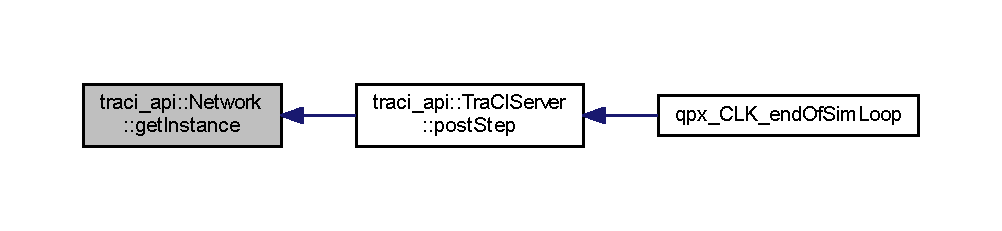
\includegraphics[width=350pt]{classtraci__api_1_1_network_ab6c12d9fa0affbeeb0d068544adb4724_icgraph}
\end{center}
\end{figure}
\mbox{\Hypertarget{classtraci__api_1_1_network_a9bfe4236d1ab692d47133c69406811b3}\label{classtraci__api_1_1_network_a9bfe4236d1ab692d47133c69406811b3}} 
\index{traci\+\_\+api\+::\+Network@{traci\+\_\+api\+::\+Network}!get\+Junction\+Variable@{get\+Junction\+Variable}}
\index{get\+Junction\+Variable@{get\+Junction\+Variable}!traci\+\_\+api\+::\+Network@{traci\+\_\+api\+::\+Network}}
\subsubsection{\texorpdfstring{get\+Junction\+Variable()}{getJunctionVariable()}}
{\footnotesize\ttfamily void traci\+\_\+api\+::\+Network\+::get\+Junction\+Variable (\begin{DoxyParamCaption}\item[{\hyperlink{classtcpip_1_1_storage}{tcpip\+::\+Storage} \&}]{input,  }\item[{\hyperlink{classtcpip_1_1_storage}{tcpip\+::\+Storage} \&}]{output }\end{DoxyParamCaption}) const throw  \hyperlink{classtraci__api_1_1_no_such_object_error}{traci\+\_\+api\+::\+No\+Such\+Object\+Error}) }

Here is the caller graph for this function\+:\nopagebreak
\begin{figure}[H]
\begin{center}
\leavevmode
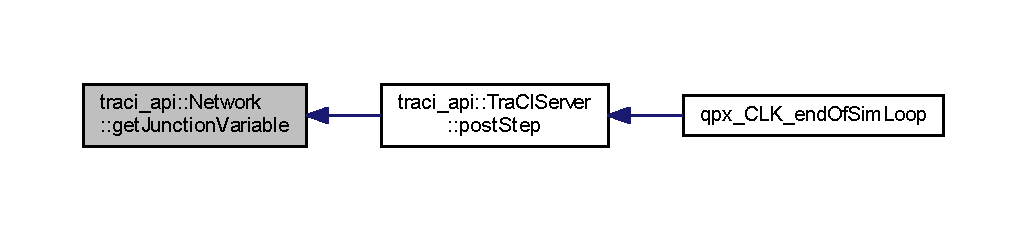
\includegraphics[width=350pt]{classtraci__api_1_1_network_a9bfe4236d1ab692d47133c69406811b3_icgraph}
\end{center}
\end{figure}
\mbox{\Hypertarget{classtraci__api_1_1_network_a8a82aa15b0422ce28ca240e88c1af4f7}\label{classtraci__api_1_1_network_a8a82aa15b0422ce28ca240e88c1af4f7}} 
\index{traci\+\_\+api\+::\+Network@{traci\+\_\+api\+::\+Network}!get\+Link\+Variable@{get\+Link\+Variable}}
\index{get\+Link\+Variable@{get\+Link\+Variable}!traci\+\_\+api\+::\+Network@{traci\+\_\+api\+::\+Network}}
\subsubsection{\texorpdfstring{get\+Link\+Variable()}{getLinkVariable()}}
{\footnotesize\ttfamily void traci\+\_\+api\+::\+Network\+::get\+Link\+Variable (\begin{DoxyParamCaption}\item[{\hyperlink{classtcpip_1_1_storage}{tcpip\+::\+Storage} \&}]{input,  }\item[{\hyperlink{classtcpip_1_1_storage}{tcpip\+::\+Storage} \&}]{output }\end{DoxyParamCaption}) const throw  \hyperlink{classtraci__api_1_1_no_such_object_error}{traci\+\_\+api\+::\+No\+Such\+Object\+Error}) }

Here is the caller graph for this function\+:\nopagebreak
\begin{figure}[H]
\begin{center}
\leavevmode
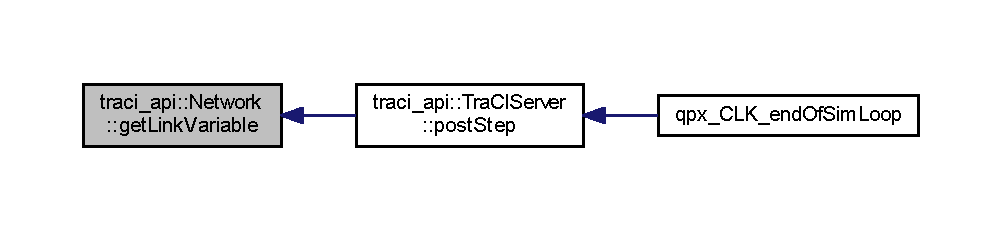
\includegraphics[width=350pt]{classtraci__api_1_1_network_a8a82aa15b0422ce28ca240e88c1af4f7_icgraph}
\end{center}
\end{figure}
\mbox{\Hypertarget{classtraci__api_1_1_network_abc0574b41332ec15856e2e5bb9926be9}\label{classtraci__api_1_1_network_abc0574b41332ec15856e2e5bb9926be9}} 
\index{traci\+\_\+api\+::\+Network@{traci\+\_\+api\+::\+Network}!get\+Route\+Variable@{get\+Route\+Variable}}
\index{get\+Route\+Variable@{get\+Route\+Variable}!traci\+\_\+api\+::\+Network@{traci\+\_\+api\+::\+Network}}
\subsubsection{\texorpdfstring{get\+Route\+Variable()}{getRouteVariable()}}
{\footnotesize\ttfamily void traci\+\_\+api\+::\+Network\+::get\+Route\+Variable (\begin{DoxyParamCaption}\item[{\hyperlink{classtcpip_1_1_storage}{tcpip\+::\+Storage} \&}]{input,  }\item[{\hyperlink{classtcpip_1_1_storage}{tcpip\+::\+Storage} \&}]{output }\end{DoxyParamCaption}) const throw  \hyperlink{classtraci__api_1_1_no_such_object_error}{traci\+\_\+api\+::\+No\+Such\+Object\+Error}) }

Here is the caller graph for this function\+:\nopagebreak
\begin{figure}[H]
\begin{center}
\leavevmode
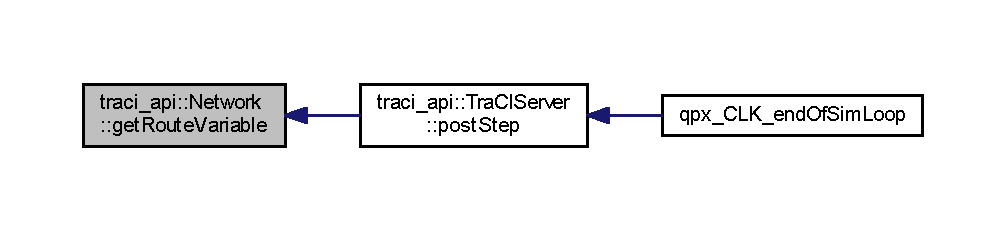
\includegraphics[width=350pt]{classtraci__api_1_1_network_abc0574b41332ec15856e2e5bb9926be9_icgraph}
\end{center}
\end{figure}
\mbox{\Hypertarget{classtraci__api_1_1_network_ae6ac9267db1ace8c368a48a7b92ce964}\label{classtraci__api_1_1_network_ae6ac9267db1ace8c368a48a7b92ce964}} 
\index{traci\+\_\+api\+::\+Network@{traci\+\_\+api\+::\+Network}!operator=@{operator=}}
\index{operator=@{operator=}!traci\+\_\+api\+::\+Network@{traci\+\_\+api\+::\+Network}}
\subsubsection{\texorpdfstring{operator=()}{operator=()}}
{\footnotesize\ttfamily void traci\+\_\+api\+::\+Network\+::operator= (\begin{DoxyParamCaption}\item[{\hyperlink{classtraci__api_1_1_network}{Network} const \&}]{ }\end{DoxyParamCaption})\hspace{0.3cm}{\ttfamily [delete]}}



The documentation for this class was generated from the following files\+:\begin{DoxyCompactItemize}
\item 
C\+:/\+Users/\+Public/paramics/programmer/plugins/pveins/src/\+Tra\+C\+I\+A\+P\+I/\hyperlink{_network_8h}{Network.\+h}\item 
C\+:/\+Users/\+Public/paramics/programmer/plugins/pveins/src/\+Tra\+C\+I\+A\+P\+I/\hyperlink{_network_8cpp}{Network.\+cpp}\end{DoxyCompactItemize}

\hypertarget{classtraci__api_1_1_no_such_object_error}{}\section{traci\+\_\+api\+:\+:No\+Such\+Object\+Error Class Reference}
\label{classtraci__api_1_1_no_such_object_error}\index{traci\+\_\+api\+::\+No\+Such\+Object\+Error@{traci\+\_\+api\+::\+No\+Such\+Object\+Error}}


{\ttfamily \#include $<$Exceptions.\+h$>$}



Inheritance diagram for traci\+\_\+api\+:\+:No\+Such\+Object\+Error\+:\nopagebreak
\begin{figure}[H]
\begin{center}
\leavevmode
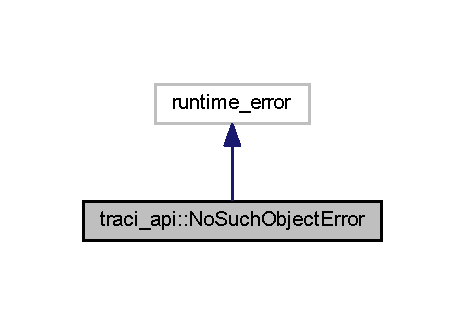
\includegraphics[width=223pt]{classtraci__api_1_1_no_such_object_error__inherit__graph}
\end{center}
\end{figure}


Collaboration diagram for traci\+\_\+api\+:\+:No\+Such\+Object\+Error\+:\nopagebreak
\begin{figure}[H]
\begin{center}
\leavevmode
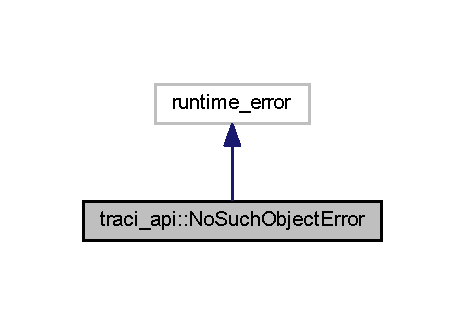
\includegraphics[width=223pt]{classtraci__api_1_1_no_such_object_error__coll__graph}
\end{center}
\end{figure}
\subsection*{Public Member Functions}
\begin{DoxyCompactItemize}
\item 
\hyperlink{classtraci__api_1_1_no_such_object_error_aebe9140c2931a0e35c5b51bbc9c511ef}{No\+Such\+Object\+Error} (const std\+::string \&\+\_\+\+Message)
\item 
\hyperlink{classtraci__api_1_1_no_such_object_error_af616a893c0094adf1d46bd3fa0664c62}{No\+Such\+Object\+Error} (const char $\ast$\+\_\+\+Message)
\end{DoxyCompactItemize}


\subsection{Constructor \& Destructor Documentation}
\mbox{\Hypertarget{classtraci__api_1_1_no_such_object_error_aebe9140c2931a0e35c5b51bbc9c511ef}\label{classtraci__api_1_1_no_such_object_error_aebe9140c2931a0e35c5b51bbc9c511ef}} 
\index{traci\+\_\+api\+::\+No\+Such\+Object\+Error@{traci\+\_\+api\+::\+No\+Such\+Object\+Error}!No\+Such\+Object\+Error@{No\+Such\+Object\+Error}}
\index{No\+Such\+Object\+Error@{No\+Such\+Object\+Error}!traci\+\_\+api\+::\+No\+Such\+Object\+Error@{traci\+\_\+api\+::\+No\+Such\+Object\+Error}}
\subsubsection{\texorpdfstring{No\+Such\+Object\+Error()}{NoSuchObjectError()}\hspace{0.1cm}{\footnotesize\ttfamily [1/2]}}
{\footnotesize\ttfamily traci\+\_\+api\+::\+No\+Such\+Object\+Error\+::\+No\+Such\+Object\+Error (\begin{DoxyParamCaption}\item[{const std\+::string \&}]{\+\_\+\+Message }\end{DoxyParamCaption})\hspace{0.3cm}{\ttfamily [inline]}, {\ttfamily [explicit]}}

\mbox{\Hypertarget{classtraci__api_1_1_no_such_object_error_af616a893c0094adf1d46bd3fa0664c62}\label{classtraci__api_1_1_no_such_object_error_af616a893c0094adf1d46bd3fa0664c62}} 
\index{traci\+\_\+api\+::\+No\+Such\+Object\+Error@{traci\+\_\+api\+::\+No\+Such\+Object\+Error}!No\+Such\+Object\+Error@{No\+Such\+Object\+Error}}
\index{No\+Such\+Object\+Error@{No\+Such\+Object\+Error}!traci\+\_\+api\+::\+No\+Such\+Object\+Error@{traci\+\_\+api\+::\+No\+Such\+Object\+Error}}
\subsubsection{\texorpdfstring{No\+Such\+Object\+Error()}{NoSuchObjectError()}\hspace{0.1cm}{\footnotesize\ttfamily [2/2]}}
{\footnotesize\ttfamily traci\+\_\+api\+::\+No\+Such\+Object\+Error\+::\+No\+Such\+Object\+Error (\begin{DoxyParamCaption}\item[{const char $\ast$}]{\+\_\+\+Message }\end{DoxyParamCaption})\hspace{0.3cm}{\ttfamily [inline]}, {\ttfamily [explicit]}}



The documentation for this class was generated from the following file\+:\begin{DoxyCompactItemize}
\item 
C\+:/\+Users/\+Public/paramics/programmer/plugins/pveins/src/\+Tra\+C\+I\+A\+P\+I/\hyperlink{_exceptions_8h}{Exceptions.\+h}\end{DoxyCompactItemize}

\hypertarget{classtraci__api_1_1_not_implemented_error}{}\section{traci\+\_\+api\+:\+:Not\+Implemented\+Error Class Reference}
\label{classtraci__api_1_1_not_implemented_error}\index{traci\+\_\+api\+::\+Not\+Implemented\+Error@{traci\+\_\+api\+::\+Not\+Implemented\+Error}}


{\ttfamily \#include $<$Exceptions.\+h$>$}



Inheritance diagram for traci\+\_\+api\+:\+:Not\+Implemented\+Error\+:\nopagebreak
\begin{figure}[H]
\begin{center}
\leavevmode
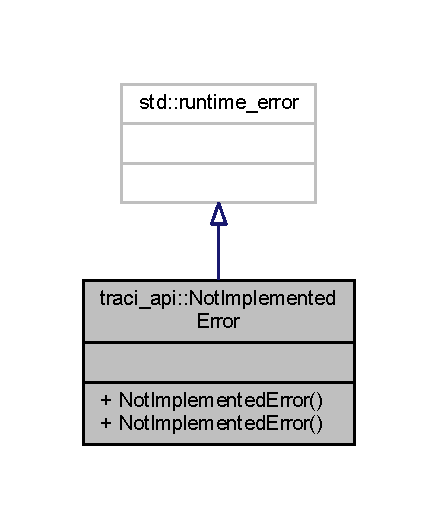
\includegraphics[width=210pt]{classtraci__api_1_1_not_implemented_error__inherit__graph}
\end{center}
\end{figure}


Collaboration diagram for traci\+\_\+api\+:\+:Not\+Implemented\+Error\+:\nopagebreak
\begin{figure}[H]
\begin{center}
\leavevmode
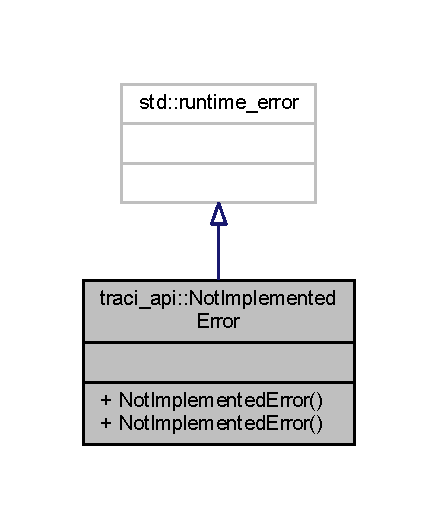
\includegraphics[width=210pt]{classtraci__api_1_1_not_implemented_error__coll__graph}
\end{center}
\end{figure}
\subsection*{Public Member Functions}
\begin{DoxyCompactItemize}
\item 
\hyperlink{classtraci__api_1_1_not_implemented_error_a1f4724cf7803566ff8171f1d855e1a95}{Not\+Implemented\+Error} (const std\+::string \&\+\_\+\+Message)
\item 
\hyperlink{classtraci__api_1_1_not_implemented_error_af8a8d5dd1656fdb6d743ade736f4faff}{Not\+Implemented\+Error} (const char $\ast$\+\_\+\+Message)
\end{DoxyCompactItemize}


\subsection{Constructor \& Destructor Documentation}
\mbox{\Hypertarget{classtraci__api_1_1_not_implemented_error_a1f4724cf7803566ff8171f1d855e1a95}\label{classtraci__api_1_1_not_implemented_error_a1f4724cf7803566ff8171f1d855e1a95}} 
\index{traci\+\_\+api\+::\+Not\+Implemented\+Error@{traci\+\_\+api\+::\+Not\+Implemented\+Error}!Not\+Implemented\+Error@{Not\+Implemented\+Error}}
\index{Not\+Implemented\+Error@{Not\+Implemented\+Error}!traci\+\_\+api\+::\+Not\+Implemented\+Error@{traci\+\_\+api\+::\+Not\+Implemented\+Error}}
\subsubsection{\texorpdfstring{Not\+Implemented\+Error()}{NotImplementedError()}\hspace{0.1cm}{\footnotesize\ttfamily [1/2]}}
{\footnotesize\ttfamily traci\+\_\+api\+::\+Not\+Implemented\+Error\+::\+Not\+Implemented\+Error (\begin{DoxyParamCaption}\item[{const std\+::string \&}]{\+\_\+\+Message }\end{DoxyParamCaption})\hspace{0.3cm}{\ttfamily [inline]}, {\ttfamily [explicit]}}

\mbox{\Hypertarget{classtraci__api_1_1_not_implemented_error_af8a8d5dd1656fdb6d743ade736f4faff}\label{classtraci__api_1_1_not_implemented_error_af8a8d5dd1656fdb6d743ade736f4faff}} 
\index{traci\+\_\+api\+::\+Not\+Implemented\+Error@{traci\+\_\+api\+::\+Not\+Implemented\+Error}!Not\+Implemented\+Error@{Not\+Implemented\+Error}}
\index{Not\+Implemented\+Error@{Not\+Implemented\+Error}!traci\+\_\+api\+::\+Not\+Implemented\+Error@{traci\+\_\+api\+::\+Not\+Implemented\+Error}}
\subsubsection{\texorpdfstring{Not\+Implemented\+Error()}{NotImplementedError()}\hspace{0.1cm}{\footnotesize\ttfamily [2/2]}}
{\footnotesize\ttfamily traci\+\_\+api\+::\+Not\+Implemented\+Error\+::\+Not\+Implemented\+Error (\begin{DoxyParamCaption}\item[{const char $\ast$}]{\+\_\+\+Message }\end{DoxyParamCaption})\hspace{0.3cm}{\ttfamily [inline]}, {\ttfamily [explicit]}}



The documentation for this class was generated from the following file\+:\begin{DoxyCompactItemize}
\item 
C\+:/\+Users/\+Public/paramics/programmer/plugins/pveins/src/\+Tra\+C\+I\+A\+P\+I/\hyperlink{_exceptions_8h}{Exceptions.\+h}\end{DoxyCompactItemize}

\hypertarget{class_positional_data}{}\section{Positional\+Data Class Reference}
\label{class_positional_data}\index{Positional\+Data@{Positional\+Data}}


{\ttfamily \#include $<$Utils.\+h$>$}



Inheritance diagram for Positional\+Data\+:
\nopagebreak
\begin{figure}[H]
\begin{center}
\leavevmode
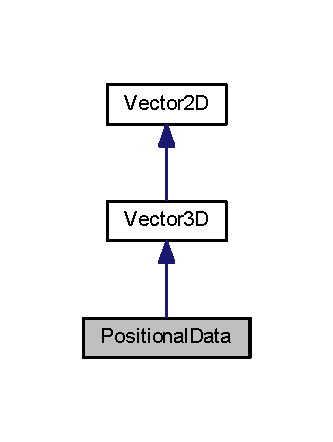
\includegraphics[width=175pt]{class_positional_data__inherit__graph}
\end{center}
\end{figure}


Collaboration diagram for Positional\+Data\+:
\nopagebreak
\begin{figure}[H]
\begin{center}
\leavevmode
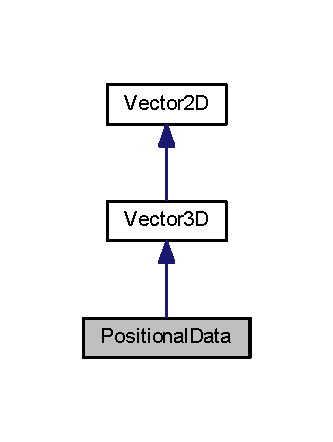
\includegraphics[width=175pt]{class_positional_data__coll__graph}
\end{center}
\end{figure}
\subsection*{Public Member Functions}
\begin{DoxyCompactItemize}
\item 
\hyperlink{class_positional_data_a31b77f08d0a18c72e3b21cac6bc2d095}{Positional\+Data} (double \hyperlink{class_vector2_d_ac5c4e553815737aa24bec8281270178f}{x}, double \hyperlink{class_vector2_d_ac38d0179cfe74c30fee290a703ab209a}{y}, double \hyperlink{class_vector3_d_a7321f3ff785f275c4d83f7d1b951752a}{z}, double b, double g)
\end{DoxyCompactItemize}
\subsection*{Public Attributes}
\begin{DoxyCompactItemize}
\item 
double \hyperlink{class_positional_data_a2aa73f7333432a8b32d2036f4c940ff3}{gradient}
\item 
double \hyperlink{class_positional_data_a2ae5a622a025a392acfb29c66e6c310e}{bearing}
\end{DoxyCompactItemize}


\subsection{Constructor \& Destructor Documentation}
\mbox{\Hypertarget{class_positional_data_a31b77f08d0a18c72e3b21cac6bc2d095}\label{class_positional_data_a31b77f08d0a18c72e3b21cac6bc2d095}} 
\index{Positional\+Data@{Positional\+Data}!Positional\+Data@{Positional\+Data}}
\index{Positional\+Data@{Positional\+Data}!Positional\+Data@{Positional\+Data}}
\subsubsection{\texorpdfstring{Positional\+Data()}{PositionalData()}}
{\footnotesize\ttfamily Positional\+Data\+::\+Positional\+Data (\begin{DoxyParamCaption}\item[{double}]{x,  }\item[{double}]{y,  }\item[{double}]{z,  }\item[{double}]{b,  }\item[{double}]{g }\end{DoxyParamCaption})\hspace{0.3cm}{\ttfamily [inline]}}



\subsection{Member Data Documentation}
\mbox{\Hypertarget{class_positional_data_a2ae5a622a025a392acfb29c66e6c310e}\label{class_positional_data_a2ae5a622a025a392acfb29c66e6c310e}} 
\index{Positional\+Data@{Positional\+Data}!bearing@{bearing}}
\index{bearing@{bearing}!Positional\+Data@{Positional\+Data}}
\subsubsection{\texorpdfstring{bearing}{bearing}}
{\footnotesize\ttfamily double Positional\+Data\+::bearing}

\mbox{\Hypertarget{class_positional_data_a2aa73f7333432a8b32d2036f4c940ff3}\label{class_positional_data_a2aa73f7333432a8b32d2036f4c940ff3}} 
\index{Positional\+Data@{Positional\+Data}!gradient@{gradient}}
\index{gradient@{gradient}!Positional\+Data@{Positional\+Data}}
\subsubsection{\texorpdfstring{gradient}{gradient}}
{\footnotesize\ttfamily double Positional\+Data\+::gradient}



The documentation for this class was generated from the following file\+:\begin{DoxyCompactItemize}
\item 
C\+:/\+Users/\+Public/paramics/programmer/plugins/pveins/src/\+Tra\+C\+I\+A\+P\+I/\hyperlink{_utils_8h}{Utils.\+h}\end{DoxyCompactItemize}

\hypertarget{classtraci__api_1_1_simulation}{}\section{traci\+\_\+api\+:\+:Simulation Class Reference}
\label{classtraci__api_1_1_simulation}\index{traci\+\_\+api\+::\+Simulation@{traci\+\_\+api\+::\+Simulation}}


{\ttfamily \#include $<$Simulation.\+h$>$}

\subsection*{Public Member Functions}
\begin{DoxyCompactItemize}
\item 
\hyperlink{classtraci__api_1_1_simulation_af0680bb9b12ef4c4d47e45f3aeebc108}{$\sim$\+Simulation} ()
\item 
\hyperlink{classtraci__api_1_1_simulation_a0e41f9a2911b8f3545002220027a9922}{Simulation} (\hyperlink{classtraci__api_1_1_simulation}{Simulation} const \&)=delete
\item 
void \hyperlink{classtraci__api_1_1_simulation_ad51b13fbeca39505efcb2171212ec99d}{operator=} (\hyperlink{classtraci__api_1_1_simulation}{Simulation} const \&)=delete
\item 
bool \hyperlink{classtraci__api_1_1_simulation_aa795b446802e3ddb196ebd29a215005e}{pack\+Simulation\+Variable} (uint8\+\_\+t var\+ID, \hyperlink{classtcpip_1_1_storage}{tcpip\+::\+Storage} \&result\+\_\+store)
\item 
void \hyperlink{classtraci__api_1_1_simulation_aa7ebe041dd0f34ccef7f2f2293775c3b}{get\+Simulation\+Variable} (uint8\+\_\+t var\+ID, \hyperlink{classtcpip_1_1_storage}{tcpip\+::\+Storage} \&result)
\item 
float \hyperlink{classtraci__api_1_1_simulation_a8e9cc88461dfab200eabf626fcdb8280}{get\+Current\+Time\+Seconds} ()
\item 
int \hyperlink{classtraci__api_1_1_simulation_a43ce3d282a312c2e6735cdcd4343b0a7}{get\+Current\+Time\+Milliseconds} ()
\item 
int \hyperlink{classtraci__api_1_1_simulation_a413eac30f40f25fabbd94cc6ff16a51c}{get\+Time\+Step\+Size\+Milliseconds} ()
\item 
void \hyperlink{classtraci__api_1_1_simulation_a1124e65809e0e3f6109654de9b28daf8}{get\+Real\+Network\+Bounds} (double \&llx, double \&lly, double \&urx, double \&ury)
\end{DoxyCompactItemize}
\subsection*{Static Public Member Functions}
\begin{DoxyCompactItemize}
\item 
static \hyperlink{classtraci__api_1_1_simulation}{Simulation} $\ast$ \hyperlink{classtraci__api_1_1_simulation_a5bd3febd1571525c2dac2b68e37f694e}{get\+Instance} ()
\item 
static void \hyperlink{classtraci__api_1_1_simulation_a952c6f62a424d4f8d3ee016dc8c935bd}{delete\+Instance} ()
\end{DoxyCompactItemize}
\subsection*{Static Public Attributes}
\begin{DoxyCompactItemize}
\item 
static const uint8\+\_\+t \hyperlink{classtraci__api_1_1_simulation_ad85a2daa3b6e62afebf23c63aa54c5a7}{V\+A\+R\+\_\+\+S\+I\+M\+T\+I\+ME} = 0x70
\item 
static const uint8\+\_\+t \hyperlink{classtraci__api_1_1_simulation_a0c320b73a88c6bd0d5d15b9b7d8ca079}{V\+A\+R\+\_\+\+L\+O\+A\+D\+E\+D\+V\+H\+C\+\_\+\+C\+NT} = 0x71
\item 
static const uint8\+\_\+t \hyperlink{classtraci__api_1_1_simulation_aef180578795a463be2e4b4d47674f07e}{V\+A\+R\+\_\+\+L\+O\+A\+D\+E\+D\+V\+H\+C\+\_\+\+L\+ST} = 0x72
\item 
static const uint8\+\_\+t \hyperlink{classtraci__api_1_1_simulation_a2211a9befd772188a83012e61d0bf890}{V\+A\+R\+\_\+\+D\+E\+P\+A\+R\+T\+E\+D\+V\+H\+C\+\_\+\+C\+NT} = 0x73
\item 
static const uint8\+\_\+t \hyperlink{classtraci__api_1_1_simulation_a4e5cf74cd62df38b5e0a4e750983c6e1}{V\+A\+R\+\_\+\+D\+E\+P\+A\+R\+T\+E\+D\+V\+H\+C\+\_\+\+L\+ST} = 0x74
\item 
static const uint8\+\_\+t \hyperlink{classtraci__api_1_1_simulation_aa2763aba4aa46ba82dc9b1f258101ca4}{V\+A\+R\+\_\+\+A\+R\+R\+I\+V\+E\+D\+V\+H\+C\+\_\+\+C\+NT} = 0x79
\item 
static const uint8\+\_\+t \hyperlink{classtraci__api_1_1_simulation_ae7a55aa19afe46dd3e54ed60ccc736bf}{V\+A\+R\+\_\+\+A\+R\+R\+I\+V\+E\+D\+V\+H\+C\+\_\+\+L\+ST} = 0x7a
\item 
static const uint8\+\_\+t \hyperlink{classtraci__api_1_1_simulation_a32191847f48857d89c02e27c7134e862}{V\+A\+R\+\_\+\+T\+I\+M\+E\+S\+T\+E\+P\+SZ} = 0x7b
\item 
static const uint8\+\_\+t \hyperlink{classtraci__api_1_1_simulation_aae0a592bee89106e697c1eb2bb312b74}{V\+A\+R\+\_\+\+N\+E\+T\+W\+O\+R\+K\+B\+N\+DS} = 0x7c
\item 
static const uint8\+\_\+t \hyperlink{classtraci__api_1_1_simulation_ad9ea6052e8bbce54c86cccd34d949859}{V\+A\+R\+\_\+\+V\+H\+C\+S\+T\+A\+R\+T\+T\+E\+L\+E\+P\+O\+R\+T\+\_\+\+C\+NT} = 0x75
\item 
static const uint8\+\_\+t \hyperlink{classtraci__api_1_1_simulation_a143172fa14c4207f49e634c7b2624627}{V\+A\+R\+\_\+\+V\+H\+C\+S\+T\+A\+R\+T\+T\+E\+L\+E\+P\+O\+R\+T\+\_\+\+L\+ST} = 0x76
\item 
static const uint8\+\_\+t \hyperlink{classtraci__api_1_1_simulation_a005529f94d02779594428533d622b5bd}{V\+A\+R\+\_\+\+V\+H\+C\+E\+N\+D\+T\+E\+L\+E\+P\+O\+R\+T\+\_\+\+C\+NT} = 0x77
\item 
static const uint8\+\_\+t \hyperlink{classtraci__api_1_1_simulation_a7662449bf431cf2c454d192f7b6c6bf8}{V\+A\+R\+\_\+\+V\+H\+C\+E\+N\+D\+T\+E\+L\+E\+P\+O\+R\+T\+\_\+\+L\+ST} = 0x78
\item 
static const uint8\+\_\+t \hyperlink{classtraci__api_1_1_simulation_afb8883f64f8a38cc0fab2ceb5ca19b12}{V\+A\+R\+\_\+\+V\+H\+C\+S\+T\+A\+R\+T\+P\+A\+R\+K\+\_\+\+C\+NT} = 0x6c
\item 
static const uint8\+\_\+t \hyperlink{classtraci__api_1_1_simulation_aa9a559c39436fc08695c37e9939d5ab4}{V\+A\+R\+\_\+\+V\+H\+C\+S\+T\+A\+R\+T\+P\+A\+R\+K\+\_\+\+L\+ST} = 0x6d
\item 
static const uint8\+\_\+t \hyperlink{classtraci__api_1_1_simulation_a6a63c336454d76895435d70b0119d2de}{V\+A\+R\+\_\+\+V\+H\+C\+E\+N\+D\+P\+A\+R\+K\+\_\+\+C\+NT} = 0x6e
\item 
static const uint8\+\_\+t \hyperlink{classtraci__api_1_1_simulation_ac9b1a6baea01106e4c283f9d8a3d40dc}{V\+A\+R\+\_\+\+V\+H\+C\+E\+N\+D\+P\+A\+R\+K\+\_\+\+L\+ST} = 0x6f
\end{DoxyCompactItemize}


\subsection{Constructor \& Destructor Documentation}
\mbox{\Hypertarget{classtraci__api_1_1_simulation_af0680bb9b12ef4c4d47e45f3aeebc108}\label{classtraci__api_1_1_simulation_af0680bb9b12ef4c4d47e45f3aeebc108}} 
\index{traci\+\_\+api\+::\+Simulation@{traci\+\_\+api\+::\+Simulation}!````~Simulation@{$\sim$\+Simulation}}
\index{````~Simulation@{$\sim$\+Simulation}!traci\+\_\+api\+::\+Simulation@{traci\+\_\+api\+::\+Simulation}}
\subsubsection{\texorpdfstring{$\sim$\+Simulation()}{~Simulation()}}
{\footnotesize\ttfamily traci\+\_\+api\+::\+Simulation\+::$\sim$\+Simulation (\begin{DoxyParamCaption}{ }\end{DoxyParamCaption})}

\mbox{\Hypertarget{classtraci__api_1_1_simulation_a0e41f9a2911b8f3545002220027a9922}\label{classtraci__api_1_1_simulation_a0e41f9a2911b8f3545002220027a9922}} 
\index{traci\+\_\+api\+::\+Simulation@{traci\+\_\+api\+::\+Simulation}!Simulation@{Simulation}}
\index{Simulation@{Simulation}!traci\+\_\+api\+::\+Simulation@{traci\+\_\+api\+::\+Simulation}}
\subsubsection{\texorpdfstring{Simulation()}{Simulation()}}
{\footnotesize\ttfamily traci\+\_\+api\+::\+Simulation\+::\+Simulation (\begin{DoxyParamCaption}\item[{\hyperlink{classtraci__api_1_1_simulation}{Simulation} const \&}]{ }\end{DoxyParamCaption})\hspace{0.3cm}{\ttfamily [delete]}}



\subsection{Member Function Documentation}
\mbox{\Hypertarget{classtraci__api_1_1_simulation_a952c6f62a424d4f8d3ee016dc8c935bd}\label{classtraci__api_1_1_simulation_a952c6f62a424d4f8d3ee016dc8c935bd}} 
\index{traci\+\_\+api\+::\+Simulation@{traci\+\_\+api\+::\+Simulation}!delete\+Instance@{delete\+Instance}}
\index{delete\+Instance@{delete\+Instance}!traci\+\_\+api\+::\+Simulation@{traci\+\_\+api\+::\+Simulation}}
\subsubsection{\texorpdfstring{delete\+Instance()}{deleteInstance()}}
{\footnotesize\ttfamily void traci\+\_\+api\+::\+Simulation\+::delete\+Instance (\begin{DoxyParamCaption}{ }\end{DoxyParamCaption})\hspace{0.3cm}{\ttfamily [static]}}

\mbox{\Hypertarget{classtraci__api_1_1_simulation_a43ce3d282a312c2e6735cdcd4343b0a7}\label{classtraci__api_1_1_simulation_a43ce3d282a312c2e6735cdcd4343b0a7}} 
\index{traci\+\_\+api\+::\+Simulation@{traci\+\_\+api\+::\+Simulation}!get\+Current\+Time\+Milliseconds@{get\+Current\+Time\+Milliseconds}}
\index{get\+Current\+Time\+Milliseconds@{get\+Current\+Time\+Milliseconds}!traci\+\_\+api\+::\+Simulation@{traci\+\_\+api\+::\+Simulation}}
\subsubsection{\texorpdfstring{get\+Current\+Time\+Milliseconds()}{getCurrentTimeMilliseconds()}}
{\footnotesize\ttfamily int traci\+\_\+api\+::\+Simulation\+::get\+Current\+Time\+Milliseconds (\begin{DoxyParamCaption}{ }\end{DoxyParamCaption})}

Here is the caller graph for this function\+:\nopagebreak
\begin{figure}[H]
\begin{center}
\leavevmode
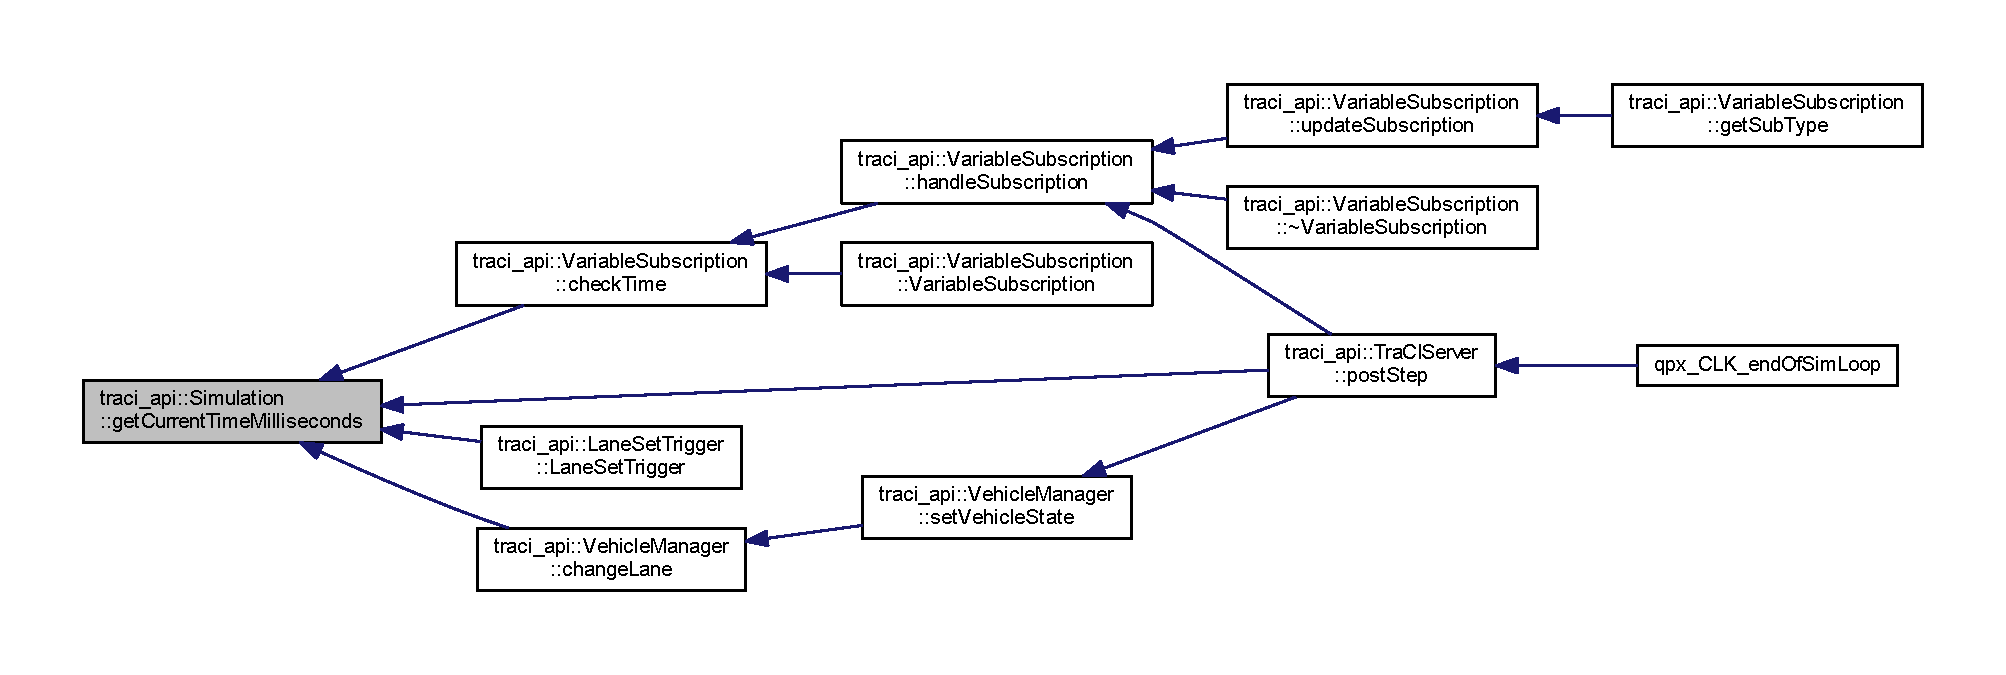
\includegraphics[width=350pt]{classtraci__api_1_1_simulation_a43ce3d282a312c2e6735cdcd4343b0a7_icgraph}
\end{center}
\end{figure}
\mbox{\Hypertarget{classtraci__api_1_1_simulation_a8e9cc88461dfab200eabf626fcdb8280}\label{classtraci__api_1_1_simulation_a8e9cc88461dfab200eabf626fcdb8280}} 
\index{traci\+\_\+api\+::\+Simulation@{traci\+\_\+api\+::\+Simulation}!get\+Current\+Time\+Seconds@{get\+Current\+Time\+Seconds}}
\index{get\+Current\+Time\+Seconds@{get\+Current\+Time\+Seconds}!traci\+\_\+api\+::\+Simulation@{traci\+\_\+api\+::\+Simulation}}
\subsubsection{\texorpdfstring{get\+Current\+Time\+Seconds()}{getCurrentTimeSeconds()}}
{\footnotesize\ttfamily float traci\+\_\+api\+::\+Simulation\+::get\+Current\+Time\+Seconds (\begin{DoxyParamCaption}{ }\end{DoxyParamCaption})}

\mbox{\Hypertarget{classtraci__api_1_1_simulation_a5bd3febd1571525c2dac2b68e37f694e}\label{classtraci__api_1_1_simulation_a5bd3febd1571525c2dac2b68e37f694e}} 
\index{traci\+\_\+api\+::\+Simulation@{traci\+\_\+api\+::\+Simulation}!get\+Instance@{get\+Instance}}
\index{get\+Instance@{get\+Instance}!traci\+\_\+api\+::\+Simulation@{traci\+\_\+api\+::\+Simulation}}
\subsubsection{\texorpdfstring{get\+Instance()}{getInstance()}}
{\footnotesize\ttfamily \hyperlink{classtraci__api_1_1_simulation}{traci\+\_\+api\+::\+Simulation} $\ast$ traci\+\_\+api\+::\+Simulation\+::get\+Instance (\begin{DoxyParamCaption}{ }\end{DoxyParamCaption})\hspace{0.3cm}{\ttfamily [static]}}

Here is the caller graph for this function\+:\nopagebreak
\begin{figure}[H]
\begin{center}
\leavevmode
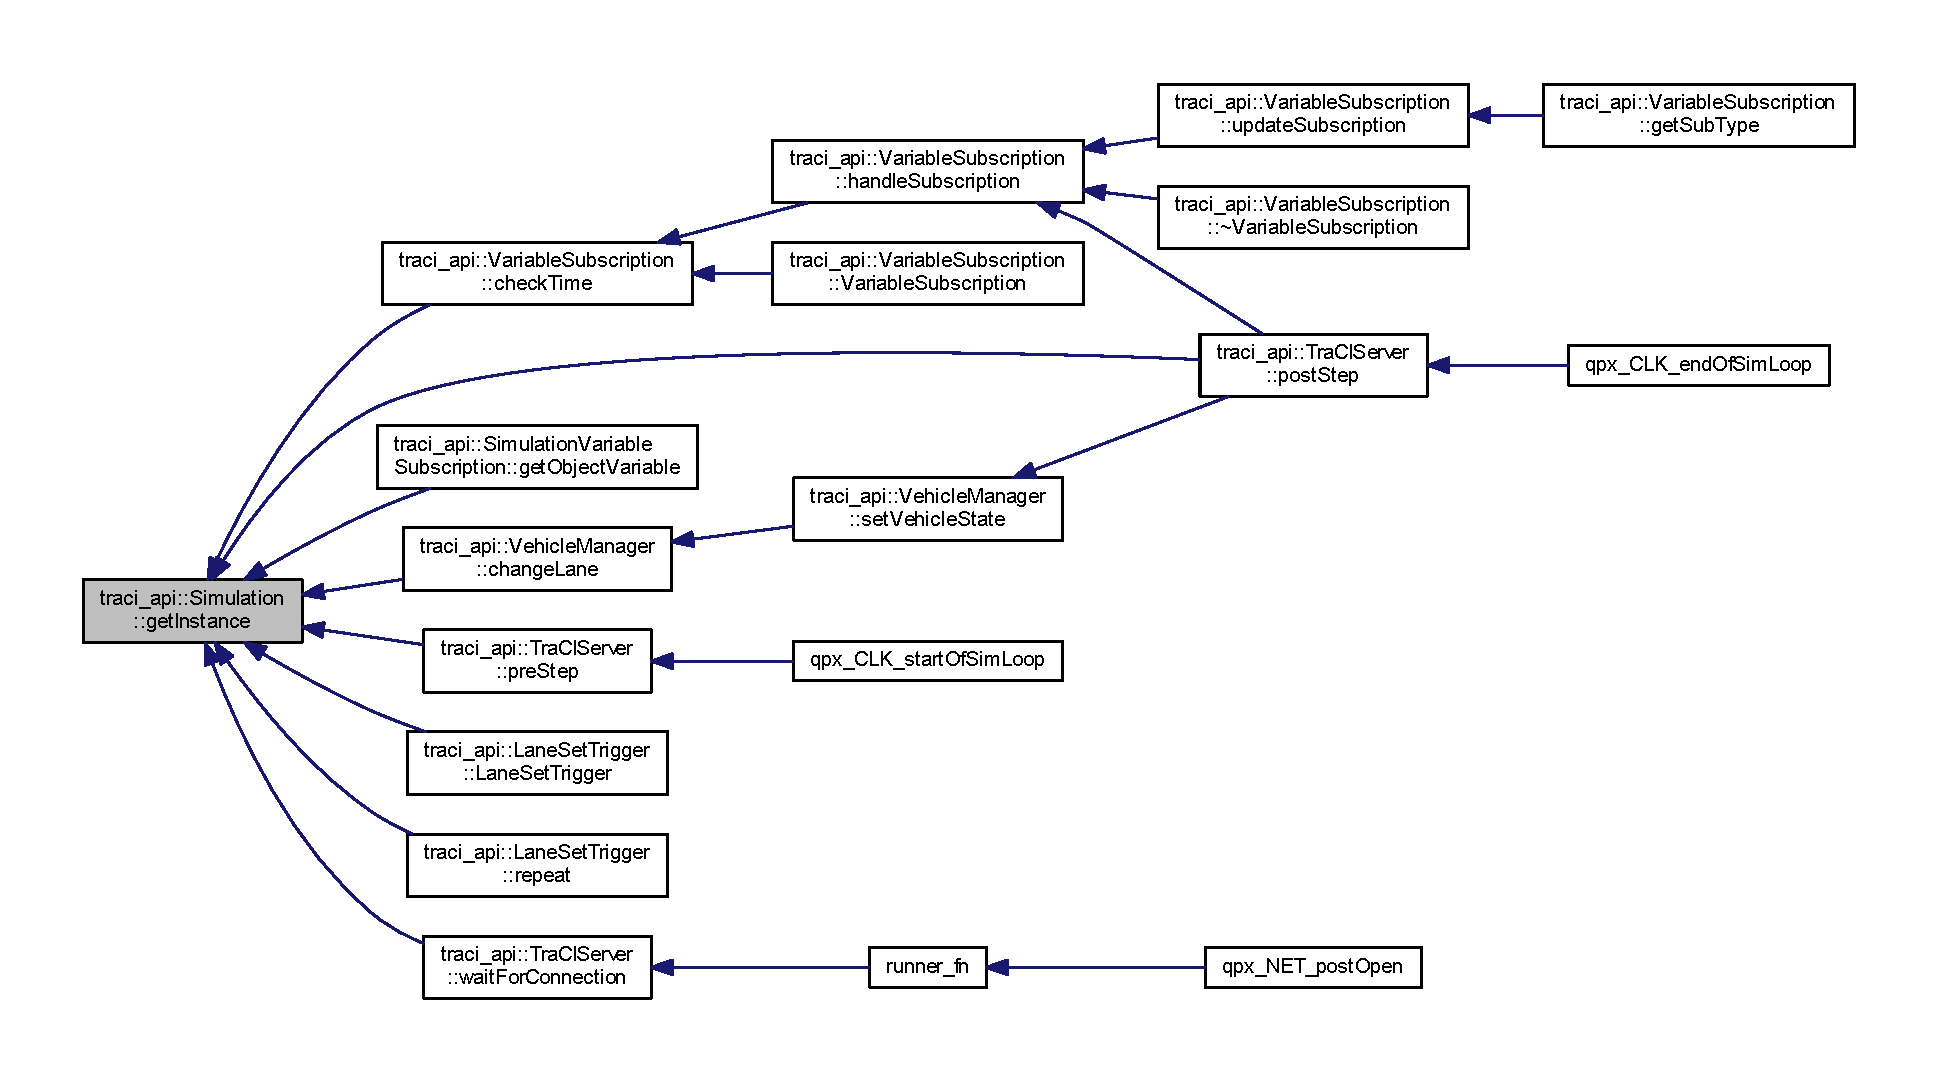
\includegraphics[width=350pt]{classtraci__api_1_1_simulation_a5bd3febd1571525c2dac2b68e37f694e_icgraph}
\end{center}
\end{figure}
\mbox{\Hypertarget{classtraci__api_1_1_simulation_a1124e65809e0e3f6109654de9b28daf8}\label{classtraci__api_1_1_simulation_a1124e65809e0e3f6109654de9b28daf8}} 
\index{traci\+\_\+api\+::\+Simulation@{traci\+\_\+api\+::\+Simulation}!get\+Real\+Network\+Bounds@{get\+Real\+Network\+Bounds}}
\index{get\+Real\+Network\+Bounds@{get\+Real\+Network\+Bounds}!traci\+\_\+api\+::\+Simulation@{traci\+\_\+api\+::\+Simulation}}
\subsubsection{\texorpdfstring{get\+Real\+Network\+Bounds()}{getRealNetworkBounds()}}
{\footnotesize\ttfamily void traci\+\_\+api\+::\+Simulation\+::get\+Real\+Network\+Bounds (\begin{DoxyParamCaption}\item[{double \&}]{llx,  }\item[{double \&}]{lly,  }\item[{double \&}]{urx,  }\item[{double \&}]{ury }\end{DoxyParamCaption})}

\mbox{\Hypertarget{classtraci__api_1_1_simulation_aa7ebe041dd0f34ccef7f2f2293775c3b}\label{classtraci__api_1_1_simulation_aa7ebe041dd0f34ccef7f2f2293775c3b}} 
\index{traci\+\_\+api\+::\+Simulation@{traci\+\_\+api\+::\+Simulation}!get\+Simulation\+Variable@{get\+Simulation\+Variable}}
\index{get\+Simulation\+Variable@{get\+Simulation\+Variable}!traci\+\_\+api\+::\+Simulation@{traci\+\_\+api\+::\+Simulation}}
\subsubsection{\texorpdfstring{get\+Simulation\+Variable()}{getSimulationVariable()}}
{\footnotesize\ttfamily void traci\+\_\+api\+::\+Simulation\+::get\+Simulation\+Variable (\begin{DoxyParamCaption}\item[{uint8\+\_\+t}]{var\+ID,  }\item[{\hyperlink{classtcpip_1_1_storage}{tcpip\+::\+Storage} \&}]{result }\end{DoxyParamCaption})}

Here is the call graph for this function\+:\nopagebreak
\begin{figure}[H]
\begin{center}
\leavevmode
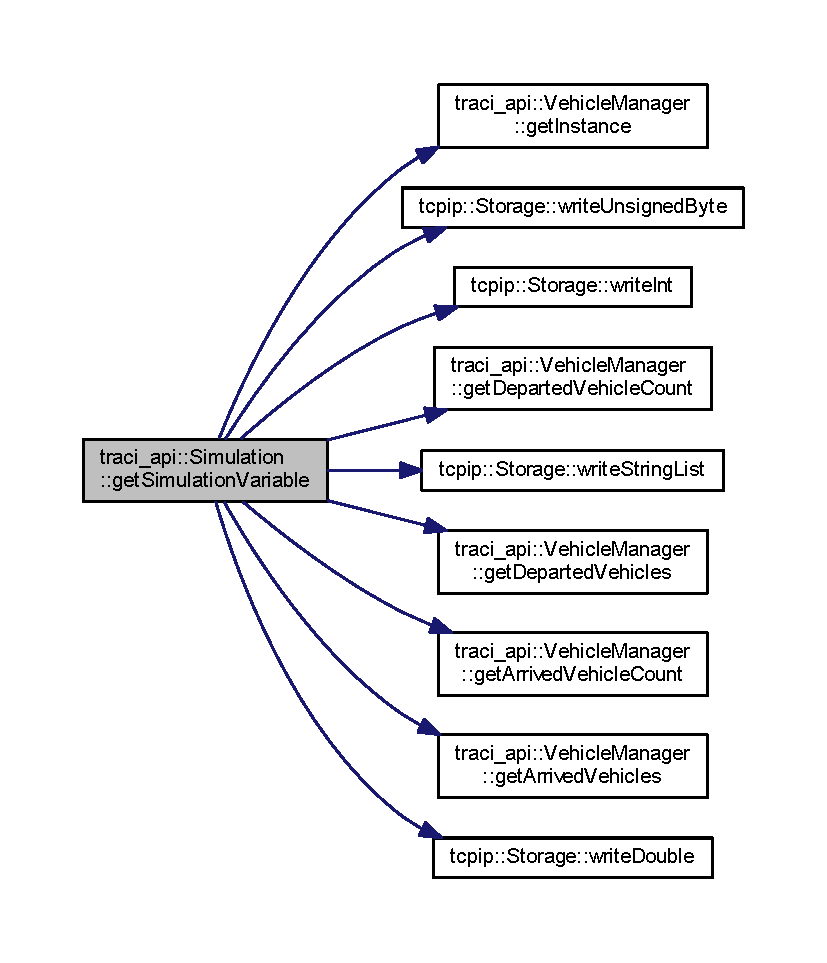
\includegraphics[width=350pt]{classtraci__api_1_1_simulation_aa7ebe041dd0f34ccef7f2f2293775c3b_cgraph}
\end{center}
\end{figure}
Here is the caller graph for this function\+:\nopagebreak
\begin{figure}[H]
\begin{center}
\leavevmode
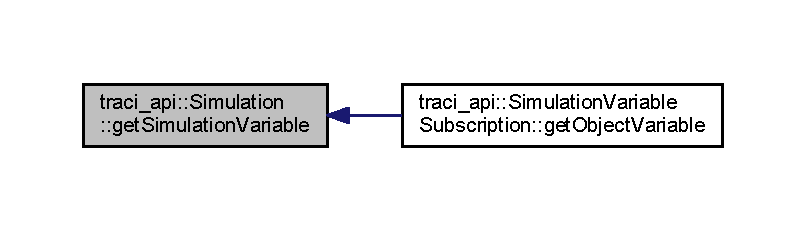
\includegraphics[width=350pt]{classtraci__api_1_1_simulation_aa7ebe041dd0f34ccef7f2f2293775c3b_icgraph}
\end{center}
\end{figure}
\mbox{\Hypertarget{classtraci__api_1_1_simulation_a413eac30f40f25fabbd94cc6ff16a51c}\label{classtraci__api_1_1_simulation_a413eac30f40f25fabbd94cc6ff16a51c}} 
\index{traci\+\_\+api\+::\+Simulation@{traci\+\_\+api\+::\+Simulation}!get\+Time\+Step\+Size\+Milliseconds@{get\+Time\+Step\+Size\+Milliseconds}}
\index{get\+Time\+Step\+Size\+Milliseconds@{get\+Time\+Step\+Size\+Milliseconds}!traci\+\_\+api\+::\+Simulation@{traci\+\_\+api\+::\+Simulation}}
\subsubsection{\texorpdfstring{get\+Time\+Step\+Size\+Milliseconds()}{getTimeStepSizeMilliseconds()}}
{\footnotesize\ttfamily int traci\+\_\+api\+::\+Simulation\+::get\+Time\+Step\+Size\+Milliseconds (\begin{DoxyParamCaption}{ }\end{DoxyParamCaption})}

Here is the caller graph for this function\+:\nopagebreak
\begin{figure}[H]
\begin{center}
\leavevmode
\includegraphics[width=350pt]{classtraci__api_1_1_simulation_a413eac30f40f25fabbd94cc6ff16a51c_icgraph}
\end{center}
\end{figure}
\mbox{\Hypertarget{classtraci__api_1_1_simulation_ad51b13fbeca39505efcb2171212ec99d}\label{classtraci__api_1_1_simulation_ad51b13fbeca39505efcb2171212ec99d}} 
\index{traci\+\_\+api\+::\+Simulation@{traci\+\_\+api\+::\+Simulation}!operator=@{operator=}}
\index{operator=@{operator=}!traci\+\_\+api\+::\+Simulation@{traci\+\_\+api\+::\+Simulation}}
\subsubsection{\texorpdfstring{operator=()}{operator=()}}
{\footnotesize\ttfamily void traci\+\_\+api\+::\+Simulation\+::operator= (\begin{DoxyParamCaption}\item[{\hyperlink{classtraci__api_1_1_simulation}{Simulation} const \&}]{ }\end{DoxyParamCaption})\hspace{0.3cm}{\ttfamily [delete]}}

\mbox{\Hypertarget{classtraci__api_1_1_simulation_aa795b446802e3ddb196ebd29a215005e}\label{classtraci__api_1_1_simulation_aa795b446802e3ddb196ebd29a215005e}} 
\index{traci\+\_\+api\+::\+Simulation@{traci\+\_\+api\+::\+Simulation}!pack\+Simulation\+Variable@{pack\+Simulation\+Variable}}
\index{pack\+Simulation\+Variable@{pack\+Simulation\+Variable}!traci\+\_\+api\+::\+Simulation@{traci\+\_\+api\+::\+Simulation}}
\subsubsection{\texorpdfstring{pack\+Simulation\+Variable()}{packSimulationVariable()}}
{\footnotesize\ttfamily bool traci\+\_\+api\+::\+Simulation\+::pack\+Simulation\+Variable (\begin{DoxyParamCaption}\item[{uint8\+\_\+t}]{var\+ID,  }\item[{\hyperlink{classtcpip_1_1_storage}{tcpip\+::\+Storage} \&}]{result\+\_\+store }\end{DoxyParamCaption})}

Here is the call graph for this function\+:\nopagebreak
\begin{figure}[H]
\begin{center}
\leavevmode
\includegraphics[width=350pt]{classtraci__api_1_1_simulation_aa795b446802e3ddb196ebd29a215005e_cgraph}
\end{center}
\end{figure}


\subsection{Member Data Documentation}
\mbox{\Hypertarget{classtraci__api_1_1_simulation_aa2763aba4aa46ba82dc9b1f258101ca4}\label{classtraci__api_1_1_simulation_aa2763aba4aa46ba82dc9b1f258101ca4}} 
\index{traci\+\_\+api\+::\+Simulation@{traci\+\_\+api\+::\+Simulation}!V\+A\+R\+\_\+\+A\+R\+R\+I\+V\+E\+D\+V\+H\+C\+\_\+\+C\+NT@{V\+A\+R\+\_\+\+A\+R\+R\+I\+V\+E\+D\+V\+H\+C\+\_\+\+C\+NT}}
\index{V\+A\+R\+\_\+\+A\+R\+R\+I\+V\+E\+D\+V\+H\+C\+\_\+\+C\+NT@{V\+A\+R\+\_\+\+A\+R\+R\+I\+V\+E\+D\+V\+H\+C\+\_\+\+C\+NT}!traci\+\_\+api\+::\+Simulation@{traci\+\_\+api\+::\+Simulation}}
\subsubsection{\texorpdfstring{V\+A\+R\+\_\+\+A\+R\+R\+I\+V\+E\+D\+V\+H\+C\+\_\+\+C\+NT}{VAR\_ARRIVEDVHC\_CNT}}
{\footnotesize\ttfamily const uint8\+\_\+t traci\+\_\+api\+::\+Simulation\+::\+V\+A\+R\+\_\+\+A\+R\+R\+I\+V\+E\+D\+V\+H\+C\+\_\+\+C\+NT = 0x79\hspace{0.3cm}{\ttfamily [static]}}

\mbox{\Hypertarget{classtraci__api_1_1_simulation_ae7a55aa19afe46dd3e54ed60ccc736bf}\label{classtraci__api_1_1_simulation_ae7a55aa19afe46dd3e54ed60ccc736bf}} 
\index{traci\+\_\+api\+::\+Simulation@{traci\+\_\+api\+::\+Simulation}!V\+A\+R\+\_\+\+A\+R\+R\+I\+V\+E\+D\+V\+H\+C\+\_\+\+L\+ST@{V\+A\+R\+\_\+\+A\+R\+R\+I\+V\+E\+D\+V\+H\+C\+\_\+\+L\+ST}}
\index{V\+A\+R\+\_\+\+A\+R\+R\+I\+V\+E\+D\+V\+H\+C\+\_\+\+L\+ST@{V\+A\+R\+\_\+\+A\+R\+R\+I\+V\+E\+D\+V\+H\+C\+\_\+\+L\+ST}!traci\+\_\+api\+::\+Simulation@{traci\+\_\+api\+::\+Simulation}}
\subsubsection{\texorpdfstring{V\+A\+R\+\_\+\+A\+R\+R\+I\+V\+E\+D\+V\+H\+C\+\_\+\+L\+ST}{VAR\_ARRIVEDVHC\_LST}}
{\footnotesize\ttfamily const uint8\+\_\+t traci\+\_\+api\+::\+Simulation\+::\+V\+A\+R\+\_\+\+A\+R\+R\+I\+V\+E\+D\+V\+H\+C\+\_\+\+L\+ST = 0x7a\hspace{0.3cm}{\ttfamily [static]}}

\mbox{\Hypertarget{classtraci__api_1_1_simulation_a2211a9befd772188a83012e61d0bf890}\label{classtraci__api_1_1_simulation_a2211a9befd772188a83012e61d0bf890}} 
\index{traci\+\_\+api\+::\+Simulation@{traci\+\_\+api\+::\+Simulation}!V\+A\+R\+\_\+\+D\+E\+P\+A\+R\+T\+E\+D\+V\+H\+C\+\_\+\+C\+NT@{V\+A\+R\+\_\+\+D\+E\+P\+A\+R\+T\+E\+D\+V\+H\+C\+\_\+\+C\+NT}}
\index{V\+A\+R\+\_\+\+D\+E\+P\+A\+R\+T\+E\+D\+V\+H\+C\+\_\+\+C\+NT@{V\+A\+R\+\_\+\+D\+E\+P\+A\+R\+T\+E\+D\+V\+H\+C\+\_\+\+C\+NT}!traci\+\_\+api\+::\+Simulation@{traci\+\_\+api\+::\+Simulation}}
\subsubsection{\texorpdfstring{V\+A\+R\+\_\+\+D\+E\+P\+A\+R\+T\+E\+D\+V\+H\+C\+\_\+\+C\+NT}{VAR\_DEPARTEDVHC\_CNT}}
{\footnotesize\ttfamily const uint8\+\_\+t traci\+\_\+api\+::\+Simulation\+::\+V\+A\+R\+\_\+\+D\+E\+P\+A\+R\+T\+E\+D\+V\+H\+C\+\_\+\+C\+NT = 0x73\hspace{0.3cm}{\ttfamily [static]}}

\mbox{\Hypertarget{classtraci__api_1_1_simulation_a4e5cf74cd62df38b5e0a4e750983c6e1}\label{classtraci__api_1_1_simulation_a4e5cf74cd62df38b5e0a4e750983c6e1}} 
\index{traci\+\_\+api\+::\+Simulation@{traci\+\_\+api\+::\+Simulation}!V\+A\+R\+\_\+\+D\+E\+P\+A\+R\+T\+E\+D\+V\+H\+C\+\_\+\+L\+ST@{V\+A\+R\+\_\+\+D\+E\+P\+A\+R\+T\+E\+D\+V\+H\+C\+\_\+\+L\+ST}}
\index{V\+A\+R\+\_\+\+D\+E\+P\+A\+R\+T\+E\+D\+V\+H\+C\+\_\+\+L\+ST@{V\+A\+R\+\_\+\+D\+E\+P\+A\+R\+T\+E\+D\+V\+H\+C\+\_\+\+L\+ST}!traci\+\_\+api\+::\+Simulation@{traci\+\_\+api\+::\+Simulation}}
\subsubsection{\texorpdfstring{V\+A\+R\+\_\+\+D\+E\+P\+A\+R\+T\+E\+D\+V\+H\+C\+\_\+\+L\+ST}{VAR\_DEPARTEDVHC\_LST}}
{\footnotesize\ttfamily const uint8\+\_\+t traci\+\_\+api\+::\+Simulation\+::\+V\+A\+R\+\_\+\+D\+E\+P\+A\+R\+T\+E\+D\+V\+H\+C\+\_\+\+L\+ST = 0x74\hspace{0.3cm}{\ttfamily [static]}}

\mbox{\Hypertarget{classtraci__api_1_1_simulation_a0c320b73a88c6bd0d5d15b9b7d8ca079}\label{classtraci__api_1_1_simulation_a0c320b73a88c6bd0d5d15b9b7d8ca079}} 
\index{traci\+\_\+api\+::\+Simulation@{traci\+\_\+api\+::\+Simulation}!V\+A\+R\+\_\+\+L\+O\+A\+D\+E\+D\+V\+H\+C\+\_\+\+C\+NT@{V\+A\+R\+\_\+\+L\+O\+A\+D\+E\+D\+V\+H\+C\+\_\+\+C\+NT}}
\index{V\+A\+R\+\_\+\+L\+O\+A\+D\+E\+D\+V\+H\+C\+\_\+\+C\+NT@{V\+A\+R\+\_\+\+L\+O\+A\+D\+E\+D\+V\+H\+C\+\_\+\+C\+NT}!traci\+\_\+api\+::\+Simulation@{traci\+\_\+api\+::\+Simulation}}
\subsubsection{\texorpdfstring{V\+A\+R\+\_\+\+L\+O\+A\+D\+E\+D\+V\+H\+C\+\_\+\+C\+NT}{VAR\_LOADEDVHC\_CNT}}
{\footnotesize\ttfamily const uint8\+\_\+t traci\+\_\+api\+::\+Simulation\+::\+V\+A\+R\+\_\+\+L\+O\+A\+D\+E\+D\+V\+H\+C\+\_\+\+C\+NT = 0x71\hspace{0.3cm}{\ttfamily [static]}}

\mbox{\Hypertarget{classtraci__api_1_1_simulation_aef180578795a463be2e4b4d47674f07e}\label{classtraci__api_1_1_simulation_aef180578795a463be2e4b4d47674f07e}} 
\index{traci\+\_\+api\+::\+Simulation@{traci\+\_\+api\+::\+Simulation}!V\+A\+R\+\_\+\+L\+O\+A\+D\+E\+D\+V\+H\+C\+\_\+\+L\+ST@{V\+A\+R\+\_\+\+L\+O\+A\+D\+E\+D\+V\+H\+C\+\_\+\+L\+ST}}
\index{V\+A\+R\+\_\+\+L\+O\+A\+D\+E\+D\+V\+H\+C\+\_\+\+L\+ST@{V\+A\+R\+\_\+\+L\+O\+A\+D\+E\+D\+V\+H\+C\+\_\+\+L\+ST}!traci\+\_\+api\+::\+Simulation@{traci\+\_\+api\+::\+Simulation}}
\subsubsection{\texorpdfstring{V\+A\+R\+\_\+\+L\+O\+A\+D\+E\+D\+V\+H\+C\+\_\+\+L\+ST}{VAR\_LOADEDVHC\_LST}}
{\footnotesize\ttfamily const uint8\+\_\+t traci\+\_\+api\+::\+Simulation\+::\+V\+A\+R\+\_\+\+L\+O\+A\+D\+E\+D\+V\+H\+C\+\_\+\+L\+ST = 0x72\hspace{0.3cm}{\ttfamily [static]}}

\mbox{\Hypertarget{classtraci__api_1_1_simulation_aae0a592bee89106e697c1eb2bb312b74}\label{classtraci__api_1_1_simulation_aae0a592bee89106e697c1eb2bb312b74}} 
\index{traci\+\_\+api\+::\+Simulation@{traci\+\_\+api\+::\+Simulation}!V\+A\+R\+\_\+\+N\+E\+T\+W\+O\+R\+K\+B\+N\+DS@{V\+A\+R\+\_\+\+N\+E\+T\+W\+O\+R\+K\+B\+N\+DS}}
\index{V\+A\+R\+\_\+\+N\+E\+T\+W\+O\+R\+K\+B\+N\+DS@{V\+A\+R\+\_\+\+N\+E\+T\+W\+O\+R\+K\+B\+N\+DS}!traci\+\_\+api\+::\+Simulation@{traci\+\_\+api\+::\+Simulation}}
\subsubsection{\texorpdfstring{V\+A\+R\+\_\+\+N\+E\+T\+W\+O\+R\+K\+B\+N\+DS}{VAR\_NETWORKBNDS}}
{\footnotesize\ttfamily const uint8\+\_\+t traci\+\_\+api\+::\+Simulation\+::\+V\+A\+R\+\_\+\+N\+E\+T\+W\+O\+R\+K\+B\+N\+DS = 0x7c\hspace{0.3cm}{\ttfamily [static]}}

\mbox{\Hypertarget{classtraci__api_1_1_simulation_ad85a2daa3b6e62afebf23c63aa54c5a7}\label{classtraci__api_1_1_simulation_ad85a2daa3b6e62afebf23c63aa54c5a7}} 
\index{traci\+\_\+api\+::\+Simulation@{traci\+\_\+api\+::\+Simulation}!V\+A\+R\+\_\+\+S\+I\+M\+T\+I\+ME@{V\+A\+R\+\_\+\+S\+I\+M\+T\+I\+ME}}
\index{V\+A\+R\+\_\+\+S\+I\+M\+T\+I\+ME@{V\+A\+R\+\_\+\+S\+I\+M\+T\+I\+ME}!traci\+\_\+api\+::\+Simulation@{traci\+\_\+api\+::\+Simulation}}
\subsubsection{\texorpdfstring{V\+A\+R\+\_\+\+S\+I\+M\+T\+I\+ME}{VAR\_SIMTIME}}
{\footnotesize\ttfamily const uint8\+\_\+t traci\+\_\+api\+::\+Simulation\+::\+V\+A\+R\+\_\+\+S\+I\+M\+T\+I\+ME = 0x70\hspace{0.3cm}{\ttfamily [static]}}

\mbox{\Hypertarget{classtraci__api_1_1_simulation_a32191847f48857d89c02e27c7134e862}\label{classtraci__api_1_1_simulation_a32191847f48857d89c02e27c7134e862}} 
\index{traci\+\_\+api\+::\+Simulation@{traci\+\_\+api\+::\+Simulation}!V\+A\+R\+\_\+\+T\+I\+M\+E\+S\+T\+E\+P\+SZ@{V\+A\+R\+\_\+\+T\+I\+M\+E\+S\+T\+E\+P\+SZ}}
\index{V\+A\+R\+\_\+\+T\+I\+M\+E\+S\+T\+E\+P\+SZ@{V\+A\+R\+\_\+\+T\+I\+M\+E\+S\+T\+E\+P\+SZ}!traci\+\_\+api\+::\+Simulation@{traci\+\_\+api\+::\+Simulation}}
\subsubsection{\texorpdfstring{V\+A\+R\+\_\+\+T\+I\+M\+E\+S\+T\+E\+P\+SZ}{VAR\_TIMESTEPSZ}}
{\footnotesize\ttfamily const uint8\+\_\+t traci\+\_\+api\+::\+Simulation\+::\+V\+A\+R\+\_\+\+T\+I\+M\+E\+S\+T\+E\+P\+SZ = 0x7b\hspace{0.3cm}{\ttfamily [static]}}

\mbox{\Hypertarget{classtraci__api_1_1_simulation_a6a63c336454d76895435d70b0119d2de}\label{classtraci__api_1_1_simulation_a6a63c336454d76895435d70b0119d2de}} 
\index{traci\+\_\+api\+::\+Simulation@{traci\+\_\+api\+::\+Simulation}!V\+A\+R\+\_\+\+V\+H\+C\+E\+N\+D\+P\+A\+R\+K\+\_\+\+C\+NT@{V\+A\+R\+\_\+\+V\+H\+C\+E\+N\+D\+P\+A\+R\+K\+\_\+\+C\+NT}}
\index{V\+A\+R\+\_\+\+V\+H\+C\+E\+N\+D\+P\+A\+R\+K\+\_\+\+C\+NT@{V\+A\+R\+\_\+\+V\+H\+C\+E\+N\+D\+P\+A\+R\+K\+\_\+\+C\+NT}!traci\+\_\+api\+::\+Simulation@{traci\+\_\+api\+::\+Simulation}}
\subsubsection{\texorpdfstring{V\+A\+R\+\_\+\+V\+H\+C\+E\+N\+D\+P\+A\+R\+K\+\_\+\+C\+NT}{VAR\_VHCENDPARK\_CNT}}
{\footnotesize\ttfamily const uint8\+\_\+t traci\+\_\+api\+::\+Simulation\+::\+V\+A\+R\+\_\+\+V\+H\+C\+E\+N\+D\+P\+A\+R\+K\+\_\+\+C\+NT = 0x6e\hspace{0.3cm}{\ttfamily [static]}}

\mbox{\Hypertarget{classtraci__api_1_1_simulation_ac9b1a6baea01106e4c283f9d8a3d40dc}\label{classtraci__api_1_1_simulation_ac9b1a6baea01106e4c283f9d8a3d40dc}} 
\index{traci\+\_\+api\+::\+Simulation@{traci\+\_\+api\+::\+Simulation}!V\+A\+R\+\_\+\+V\+H\+C\+E\+N\+D\+P\+A\+R\+K\+\_\+\+L\+ST@{V\+A\+R\+\_\+\+V\+H\+C\+E\+N\+D\+P\+A\+R\+K\+\_\+\+L\+ST}}
\index{V\+A\+R\+\_\+\+V\+H\+C\+E\+N\+D\+P\+A\+R\+K\+\_\+\+L\+ST@{V\+A\+R\+\_\+\+V\+H\+C\+E\+N\+D\+P\+A\+R\+K\+\_\+\+L\+ST}!traci\+\_\+api\+::\+Simulation@{traci\+\_\+api\+::\+Simulation}}
\subsubsection{\texorpdfstring{V\+A\+R\+\_\+\+V\+H\+C\+E\+N\+D\+P\+A\+R\+K\+\_\+\+L\+ST}{VAR\_VHCENDPARK\_LST}}
{\footnotesize\ttfamily const uint8\+\_\+t traci\+\_\+api\+::\+Simulation\+::\+V\+A\+R\+\_\+\+V\+H\+C\+E\+N\+D\+P\+A\+R\+K\+\_\+\+L\+ST = 0x6f\hspace{0.3cm}{\ttfamily [static]}}

\mbox{\Hypertarget{classtraci__api_1_1_simulation_a005529f94d02779594428533d622b5bd}\label{classtraci__api_1_1_simulation_a005529f94d02779594428533d622b5bd}} 
\index{traci\+\_\+api\+::\+Simulation@{traci\+\_\+api\+::\+Simulation}!V\+A\+R\+\_\+\+V\+H\+C\+E\+N\+D\+T\+E\+L\+E\+P\+O\+R\+T\+\_\+\+C\+NT@{V\+A\+R\+\_\+\+V\+H\+C\+E\+N\+D\+T\+E\+L\+E\+P\+O\+R\+T\+\_\+\+C\+NT}}
\index{V\+A\+R\+\_\+\+V\+H\+C\+E\+N\+D\+T\+E\+L\+E\+P\+O\+R\+T\+\_\+\+C\+NT@{V\+A\+R\+\_\+\+V\+H\+C\+E\+N\+D\+T\+E\+L\+E\+P\+O\+R\+T\+\_\+\+C\+NT}!traci\+\_\+api\+::\+Simulation@{traci\+\_\+api\+::\+Simulation}}
\subsubsection{\texorpdfstring{V\+A\+R\+\_\+\+V\+H\+C\+E\+N\+D\+T\+E\+L\+E\+P\+O\+R\+T\+\_\+\+C\+NT}{VAR\_VHCENDTELEPORT\_CNT}}
{\footnotesize\ttfamily const uint8\+\_\+t traci\+\_\+api\+::\+Simulation\+::\+V\+A\+R\+\_\+\+V\+H\+C\+E\+N\+D\+T\+E\+L\+E\+P\+O\+R\+T\+\_\+\+C\+NT = 0x77\hspace{0.3cm}{\ttfamily [static]}}

\mbox{\Hypertarget{classtraci__api_1_1_simulation_a7662449bf431cf2c454d192f7b6c6bf8}\label{classtraci__api_1_1_simulation_a7662449bf431cf2c454d192f7b6c6bf8}} 
\index{traci\+\_\+api\+::\+Simulation@{traci\+\_\+api\+::\+Simulation}!V\+A\+R\+\_\+\+V\+H\+C\+E\+N\+D\+T\+E\+L\+E\+P\+O\+R\+T\+\_\+\+L\+ST@{V\+A\+R\+\_\+\+V\+H\+C\+E\+N\+D\+T\+E\+L\+E\+P\+O\+R\+T\+\_\+\+L\+ST}}
\index{V\+A\+R\+\_\+\+V\+H\+C\+E\+N\+D\+T\+E\+L\+E\+P\+O\+R\+T\+\_\+\+L\+ST@{V\+A\+R\+\_\+\+V\+H\+C\+E\+N\+D\+T\+E\+L\+E\+P\+O\+R\+T\+\_\+\+L\+ST}!traci\+\_\+api\+::\+Simulation@{traci\+\_\+api\+::\+Simulation}}
\subsubsection{\texorpdfstring{V\+A\+R\+\_\+\+V\+H\+C\+E\+N\+D\+T\+E\+L\+E\+P\+O\+R\+T\+\_\+\+L\+ST}{VAR\_VHCENDTELEPORT\_LST}}
{\footnotesize\ttfamily const uint8\+\_\+t traci\+\_\+api\+::\+Simulation\+::\+V\+A\+R\+\_\+\+V\+H\+C\+E\+N\+D\+T\+E\+L\+E\+P\+O\+R\+T\+\_\+\+L\+ST = 0x78\hspace{0.3cm}{\ttfamily [static]}}

\mbox{\Hypertarget{classtraci__api_1_1_simulation_afb8883f64f8a38cc0fab2ceb5ca19b12}\label{classtraci__api_1_1_simulation_afb8883f64f8a38cc0fab2ceb5ca19b12}} 
\index{traci\+\_\+api\+::\+Simulation@{traci\+\_\+api\+::\+Simulation}!V\+A\+R\+\_\+\+V\+H\+C\+S\+T\+A\+R\+T\+P\+A\+R\+K\+\_\+\+C\+NT@{V\+A\+R\+\_\+\+V\+H\+C\+S\+T\+A\+R\+T\+P\+A\+R\+K\+\_\+\+C\+NT}}
\index{V\+A\+R\+\_\+\+V\+H\+C\+S\+T\+A\+R\+T\+P\+A\+R\+K\+\_\+\+C\+NT@{V\+A\+R\+\_\+\+V\+H\+C\+S\+T\+A\+R\+T\+P\+A\+R\+K\+\_\+\+C\+NT}!traci\+\_\+api\+::\+Simulation@{traci\+\_\+api\+::\+Simulation}}
\subsubsection{\texorpdfstring{V\+A\+R\+\_\+\+V\+H\+C\+S\+T\+A\+R\+T\+P\+A\+R\+K\+\_\+\+C\+NT}{VAR\_VHCSTARTPARK\_CNT}}
{\footnotesize\ttfamily const uint8\+\_\+t traci\+\_\+api\+::\+Simulation\+::\+V\+A\+R\+\_\+\+V\+H\+C\+S\+T\+A\+R\+T\+P\+A\+R\+K\+\_\+\+C\+NT = 0x6c\hspace{0.3cm}{\ttfamily [static]}}

\mbox{\Hypertarget{classtraci__api_1_1_simulation_aa9a559c39436fc08695c37e9939d5ab4}\label{classtraci__api_1_1_simulation_aa9a559c39436fc08695c37e9939d5ab4}} 
\index{traci\+\_\+api\+::\+Simulation@{traci\+\_\+api\+::\+Simulation}!V\+A\+R\+\_\+\+V\+H\+C\+S\+T\+A\+R\+T\+P\+A\+R\+K\+\_\+\+L\+ST@{V\+A\+R\+\_\+\+V\+H\+C\+S\+T\+A\+R\+T\+P\+A\+R\+K\+\_\+\+L\+ST}}
\index{V\+A\+R\+\_\+\+V\+H\+C\+S\+T\+A\+R\+T\+P\+A\+R\+K\+\_\+\+L\+ST@{V\+A\+R\+\_\+\+V\+H\+C\+S\+T\+A\+R\+T\+P\+A\+R\+K\+\_\+\+L\+ST}!traci\+\_\+api\+::\+Simulation@{traci\+\_\+api\+::\+Simulation}}
\subsubsection{\texorpdfstring{V\+A\+R\+\_\+\+V\+H\+C\+S\+T\+A\+R\+T\+P\+A\+R\+K\+\_\+\+L\+ST}{VAR\_VHCSTARTPARK\_LST}}
{\footnotesize\ttfamily const uint8\+\_\+t traci\+\_\+api\+::\+Simulation\+::\+V\+A\+R\+\_\+\+V\+H\+C\+S\+T\+A\+R\+T\+P\+A\+R\+K\+\_\+\+L\+ST = 0x6d\hspace{0.3cm}{\ttfamily [static]}}

\mbox{\Hypertarget{classtraci__api_1_1_simulation_ad9ea6052e8bbce54c86cccd34d949859}\label{classtraci__api_1_1_simulation_ad9ea6052e8bbce54c86cccd34d949859}} 
\index{traci\+\_\+api\+::\+Simulation@{traci\+\_\+api\+::\+Simulation}!V\+A\+R\+\_\+\+V\+H\+C\+S\+T\+A\+R\+T\+T\+E\+L\+E\+P\+O\+R\+T\+\_\+\+C\+NT@{V\+A\+R\+\_\+\+V\+H\+C\+S\+T\+A\+R\+T\+T\+E\+L\+E\+P\+O\+R\+T\+\_\+\+C\+NT}}
\index{V\+A\+R\+\_\+\+V\+H\+C\+S\+T\+A\+R\+T\+T\+E\+L\+E\+P\+O\+R\+T\+\_\+\+C\+NT@{V\+A\+R\+\_\+\+V\+H\+C\+S\+T\+A\+R\+T\+T\+E\+L\+E\+P\+O\+R\+T\+\_\+\+C\+NT}!traci\+\_\+api\+::\+Simulation@{traci\+\_\+api\+::\+Simulation}}
\subsubsection{\texorpdfstring{V\+A\+R\+\_\+\+V\+H\+C\+S\+T\+A\+R\+T\+T\+E\+L\+E\+P\+O\+R\+T\+\_\+\+C\+NT}{VAR\_VHCSTARTTELEPORT\_CNT}}
{\footnotesize\ttfamily const uint8\+\_\+t traci\+\_\+api\+::\+Simulation\+::\+V\+A\+R\+\_\+\+V\+H\+C\+S\+T\+A\+R\+T\+T\+E\+L\+E\+P\+O\+R\+T\+\_\+\+C\+NT = 0x75\hspace{0.3cm}{\ttfamily [static]}}

\mbox{\Hypertarget{classtraci__api_1_1_simulation_a143172fa14c4207f49e634c7b2624627}\label{classtraci__api_1_1_simulation_a143172fa14c4207f49e634c7b2624627}} 
\index{traci\+\_\+api\+::\+Simulation@{traci\+\_\+api\+::\+Simulation}!V\+A\+R\+\_\+\+V\+H\+C\+S\+T\+A\+R\+T\+T\+E\+L\+E\+P\+O\+R\+T\+\_\+\+L\+ST@{V\+A\+R\+\_\+\+V\+H\+C\+S\+T\+A\+R\+T\+T\+E\+L\+E\+P\+O\+R\+T\+\_\+\+L\+ST}}
\index{V\+A\+R\+\_\+\+V\+H\+C\+S\+T\+A\+R\+T\+T\+E\+L\+E\+P\+O\+R\+T\+\_\+\+L\+ST@{V\+A\+R\+\_\+\+V\+H\+C\+S\+T\+A\+R\+T\+T\+E\+L\+E\+P\+O\+R\+T\+\_\+\+L\+ST}!traci\+\_\+api\+::\+Simulation@{traci\+\_\+api\+::\+Simulation}}
\subsubsection{\texorpdfstring{V\+A\+R\+\_\+\+V\+H\+C\+S\+T\+A\+R\+T\+T\+E\+L\+E\+P\+O\+R\+T\+\_\+\+L\+ST}{VAR\_VHCSTARTTELEPORT\_LST}}
{\footnotesize\ttfamily const uint8\+\_\+t traci\+\_\+api\+::\+Simulation\+::\+V\+A\+R\+\_\+\+V\+H\+C\+S\+T\+A\+R\+T\+T\+E\+L\+E\+P\+O\+R\+T\+\_\+\+L\+ST = 0x76\hspace{0.3cm}{\ttfamily [static]}}



The documentation for this class was generated from the following files\+:\begin{DoxyCompactItemize}
\item 
C\+:/\+Users/\+Public/paramics/programmer/plugins/pveins/src/\+Tra\+C\+I\+A\+P\+I/\hyperlink{_simulation_8h}{Simulation.\+h}\item 
C\+:/\+Users/\+Public/paramics/programmer/plugins/pveins/src/\+Tra\+C\+I\+A\+P\+I/\hyperlink{_simulation_8cpp}{Simulation.\+cpp}\end{DoxyCompactItemize}

\hypertarget{classtraci__api_1_1_simulation_variable_subscription}{}\section{traci\+\_\+api\+:\+:Simulation\+Variable\+Subscription Class Reference}
\label{classtraci__api_1_1_simulation_variable_subscription}\index{traci\+\_\+api\+::\+Simulation\+Variable\+Subscription@{traci\+\_\+api\+::\+Simulation\+Variable\+Subscription}}


{\ttfamily \#include $<$Subscriptions.\+h$>$}



Inheritance diagram for traci\+\_\+api\+:\+:Simulation\+Variable\+Subscription\+:\nopagebreak
\begin{figure}[H]
\begin{center}
\leavevmode
\includegraphics[width=229pt]{classtraci__api_1_1_simulation_variable_subscription__inherit__graph}
\end{center}
\end{figure}


Collaboration diagram for traci\+\_\+api\+:\+:Simulation\+Variable\+Subscription\+:\nopagebreak
\begin{figure}[H]
\begin{center}
\leavevmode
\includegraphics[width=229pt]{classtraci__api_1_1_simulation_variable_subscription__coll__graph}
\end{center}
\end{figure}
\subsection*{Public Member Functions}
\begin{DoxyCompactItemize}
\item 
\hyperlink{classtraci__api_1_1_simulation_variable_subscription_a951c6d8797603b6bb73e6e78c226cf07}{Simulation\+Variable\+Subscription} (std\+::string object\+\_\+id, int begin\+\_\+time, int end\+\_\+time, const std\+::vector$<$ uint8\+\_\+t $>$ \&\hyperlink{classtraci__api_1_1_variable_subscription_a59bec6554debe2d14d75c29017561959}{vars})
\item 
\hyperlink{classtraci__api_1_1_simulation_variable_subscription_a25629e076fde526a24425f79da6523da}{$\sim$\+Simulation\+Variable\+Subscription} () override
\item 
void \hyperlink{classtraci__api_1_1_simulation_variable_subscription_aaa64f6368289ff45730d718e3f38f762}{get\+Object\+Variable} (uint8\+\_\+t var\+\_\+id, \hyperlink{classtcpip_1_1_storage}{tcpip\+::\+Storage} \&result) override
\item 
uint8\+\_\+t \hyperlink{classtraci__api_1_1_simulation_variable_subscription_a1f5a6a5d62fe7a054f87311b0c5b6f5f}{get\+Response\+Code} () const override
\end{DoxyCompactItemize}
\subsection*{Additional Inherited Members}


\subsection{Constructor \& Destructor Documentation}
\mbox{\Hypertarget{classtraci__api_1_1_simulation_variable_subscription_a951c6d8797603b6bb73e6e78c226cf07}\label{classtraci__api_1_1_simulation_variable_subscription_a951c6d8797603b6bb73e6e78c226cf07}} 
\index{traci\+\_\+api\+::\+Simulation\+Variable\+Subscription@{traci\+\_\+api\+::\+Simulation\+Variable\+Subscription}!Simulation\+Variable\+Subscription@{Simulation\+Variable\+Subscription}}
\index{Simulation\+Variable\+Subscription@{Simulation\+Variable\+Subscription}!traci\+\_\+api\+::\+Simulation\+Variable\+Subscription@{traci\+\_\+api\+::\+Simulation\+Variable\+Subscription}}
\subsubsection{\texorpdfstring{Simulation\+Variable\+Subscription()}{SimulationVariableSubscription()}}
{\footnotesize\ttfamily traci\+\_\+api\+::\+Simulation\+Variable\+Subscription\+::\+Simulation\+Variable\+Subscription (\begin{DoxyParamCaption}\item[{std\+::string}]{object\+\_\+id,  }\item[{int}]{begin\+\_\+time,  }\item[{int}]{end\+\_\+time,  }\item[{const std\+::vector$<$ uint8\+\_\+t $>$ \&}]{vars }\end{DoxyParamCaption})\hspace{0.3cm}{\ttfamily [inline]}}

\mbox{\Hypertarget{classtraci__api_1_1_simulation_variable_subscription_a25629e076fde526a24425f79da6523da}\label{classtraci__api_1_1_simulation_variable_subscription_a25629e076fde526a24425f79da6523da}} 
\index{traci\+\_\+api\+::\+Simulation\+Variable\+Subscription@{traci\+\_\+api\+::\+Simulation\+Variable\+Subscription}!````~Simulation\+Variable\+Subscription@{$\sim$\+Simulation\+Variable\+Subscription}}
\index{````~Simulation\+Variable\+Subscription@{$\sim$\+Simulation\+Variable\+Subscription}!traci\+\_\+api\+::\+Simulation\+Variable\+Subscription@{traci\+\_\+api\+::\+Simulation\+Variable\+Subscription}}
\subsubsection{\texorpdfstring{$\sim$\+Simulation\+Variable\+Subscription()}{~SimulationVariableSubscription()}}
{\footnotesize\ttfamily traci\+\_\+api\+::\+Simulation\+Variable\+Subscription\+::$\sim$\+Simulation\+Variable\+Subscription (\begin{DoxyParamCaption}{ }\end{DoxyParamCaption})\hspace{0.3cm}{\ttfamily [inline]}, {\ttfamily [override]}}

Here is the call graph for this function\+:\nopagebreak
\begin{figure}[H]
\begin{center}
\leavevmode
\includegraphics[width=350pt]{classtraci__api_1_1_simulation_variable_subscription_a25629e076fde526a24425f79da6523da_cgraph}
\end{center}
\end{figure}


\subsection{Member Function Documentation}
\mbox{\Hypertarget{classtraci__api_1_1_simulation_variable_subscription_aaa64f6368289ff45730d718e3f38f762}\label{classtraci__api_1_1_simulation_variable_subscription_aaa64f6368289ff45730d718e3f38f762}} 
\index{traci\+\_\+api\+::\+Simulation\+Variable\+Subscription@{traci\+\_\+api\+::\+Simulation\+Variable\+Subscription}!get\+Object\+Variable@{get\+Object\+Variable}}
\index{get\+Object\+Variable@{get\+Object\+Variable}!traci\+\_\+api\+::\+Simulation\+Variable\+Subscription@{traci\+\_\+api\+::\+Simulation\+Variable\+Subscription}}
\subsubsection{\texorpdfstring{get\+Object\+Variable()}{getObjectVariable()}}
{\footnotesize\ttfamily void traci\+\_\+api\+::\+Simulation\+Variable\+Subscription\+::get\+Object\+Variable (\begin{DoxyParamCaption}\item[{uint8\+\_\+t}]{var\+\_\+id,  }\item[{\hyperlink{classtcpip_1_1_storage}{tcpip\+::\+Storage} \&}]{result }\end{DoxyParamCaption})\hspace{0.3cm}{\ttfamily [override]}, {\ttfamily [virtual]}}



Implements \hyperlink{classtraci__api_1_1_variable_subscription_a884dba03a44455e86c417c3641ec6aa4}{traci\+\_\+api\+::\+Variable\+Subscription}.

Here is the call graph for this function\+:\nopagebreak
\begin{figure}[H]
\begin{center}
\leavevmode
\includegraphics[width=350pt]{classtraci__api_1_1_simulation_variable_subscription_aaa64f6368289ff45730d718e3f38f762_cgraph}
\end{center}
\end{figure}
\mbox{\Hypertarget{classtraci__api_1_1_simulation_variable_subscription_a1f5a6a5d62fe7a054f87311b0c5b6f5f}\label{classtraci__api_1_1_simulation_variable_subscription_a1f5a6a5d62fe7a054f87311b0c5b6f5f}} 
\index{traci\+\_\+api\+::\+Simulation\+Variable\+Subscription@{traci\+\_\+api\+::\+Simulation\+Variable\+Subscription}!get\+Response\+Code@{get\+Response\+Code}}
\index{get\+Response\+Code@{get\+Response\+Code}!traci\+\_\+api\+::\+Simulation\+Variable\+Subscription@{traci\+\_\+api\+::\+Simulation\+Variable\+Subscription}}
\subsubsection{\texorpdfstring{get\+Response\+Code()}{getResponseCode()}}
{\footnotesize\ttfamily uint8\+\_\+t traci\+\_\+api\+::\+Simulation\+Variable\+Subscription\+::get\+Response\+Code (\begin{DoxyParamCaption}{ }\end{DoxyParamCaption}) const\hspace{0.3cm}{\ttfamily [override]}, {\ttfamily [virtual]}}



Implements \hyperlink{classtraci__api_1_1_variable_subscription_a3e852072c435d02f96ff91f81506cef9}{traci\+\_\+api\+::\+Variable\+Subscription}.



The documentation for this class was generated from the following files\+:\begin{DoxyCompactItemize}
\item 
C\+:/\+Users/\+Public/paramics/programmer/plugins/pveins/src/\+Tra\+C\+I\+A\+P\+I/\hyperlink{_subscriptions_8h}{Subscriptions.\+h}\item 
C\+:/\+Users/\+Public/paramics/programmer/plugins/pveins/src/\+Tra\+C\+I\+A\+P\+I/\hyperlink{_subscriptions_8cpp}{Subscriptions.\+cpp}\end{DoxyCompactItemize}

\hypertarget{classtcpip_1_1_socket}{}\section{tcpip\+:\+:Socket Class Reference}
\label{classtcpip_1_1_socket}\index{tcpip\+::\+Socket@{tcpip\+::\+Socket}}


{\ttfamily \#include $<$socket.\+h$>$}

\subsection*{Public Member Functions}
\begin{DoxyCompactItemize}
\item 
\hyperlink{classtcpip_1_1_socket_adcf673cc4a6e4183f4a6f0929e13c5c1}{Socket} (std\+::string host, int \hyperlink{classtcpip_1_1_socket_ab7e67c84c32557ffb98d940081497d67}{port})
\begin{DoxyCompactList}\small\item\em Constructor that prepare to connect to host\+:port. \end{DoxyCompactList}\item 
\hyperlink{classtcpip_1_1_socket_af92b0e4bfc335b36971e94baa19fa017}{Socket} (int \hyperlink{classtcpip_1_1_socket_ab7e67c84c32557ffb98d940081497d67}{port})
\begin{DoxyCompactList}\small\item\em Constructor that prepare for accepting a connection on given port. \end{DoxyCompactList}\item 
\hyperlink{classtcpip_1_1_socket_a610c213f4b2fad07cc0bfddc3a5577e4}{$\sim$\+Socket} ()
\begin{DoxyCompactList}\small\item\em Destructor. \end{DoxyCompactList}\item 
void \hyperlink{classtcpip_1_1_socket_a8f89d187776729d15db3ba5c99c36acd}{connect} ()  throw ( Socket\+Exception)
\begin{DoxyCompactList}\small\item\em Connects to host\+\_\+\+:port\+\_\+. \end{DoxyCompactList}\item 
void \hyperlink{classtcpip_1_1_socket_a7847299f806a73798f4ceb95ab0e3d51}{accept} ()  throw ( Socket\+Exception)
\begin{DoxyCompactList}\small\item\em Wait for a incoming connection to port\+\_\+. \end{DoxyCompactList}\item 
void \hyperlink{classtcpip_1_1_socket_acb91f20e7a532159a8daa2796fa4abd4}{send} (const std\+::vector$<$ unsigned char $>$ \&buffer)  throw ( Socket\+Exception)
\item 
void \hyperlink{classtcpip_1_1_socket_a6d00027b40f48d4ae19e3fff2e89f7ab}{send\+Exact} (const \hyperlink{classtcpip_1_1_storage}{Storage} \&)  throw ( Socket\+Exception)
\item 
std\+::vector$<$ unsigned char $>$ \hyperlink{classtcpip_1_1_socket_a1da162e961fee9f1a1450df9700fd468}{receive} (int buf\+Size=2048)  throw ( Socket\+Exception)
\begin{DoxyCompactList}\small\item\em Receive up to {\ttfamily buf\+Size} available bytes from Socket\+::socket\+\_\+. \end{DoxyCompactList}\item 
bool \hyperlink{classtcpip_1_1_socket_a0d00337ac1fbad2cf183f0a651539e2e}{receive\+Exact} (\hyperlink{classtcpip_1_1_storage}{Storage} \&)  throw ( Socket\+Exception)
\begin{DoxyCompactList}\small\item\em Receive a complete Tra\+CI message from Socket\+::socket\+\_\+. \end{DoxyCompactList}\item 
void \hyperlink{classtcpip_1_1_socket_adda6f45e2b5fabc7f539f4ddcbe4b144}{close} ()
\item 
int \hyperlink{classtcpip_1_1_socket_ab7e67c84c32557ffb98d940081497d67}{port} ()
\item 
void \hyperlink{classtcpip_1_1_socket_ac382abc174bd18e4a61354cd857470c8}{set\+\_\+blocking} (bool)  throw ( Socket\+Exception)
\item 
bool \hyperlink{classtcpip_1_1_socket_a4a599332c62974235bde84f2145066b4}{is\+\_\+blocking} ()  throw ()
\item 
bool \hyperlink{classtcpip_1_1_socket_a78436cfed4ad686180491c38e88ebfc3}{has\+\_\+client\+\_\+connection} () const
\item 
bool \hyperlink{classtcpip_1_1_socket_a5633dda8e133b4eba9028b4e460b5587}{verbose} ()
\item 
void \hyperlink{classtcpip_1_1_socket_a695b2054effe2dfc2eddb12b7032b723}{set\+\_\+verbose} (bool new\+Verbose)
\end{DoxyCompactItemize}
\subsection*{Protected Member Functions}
\begin{DoxyCompactItemize}
\item 
void \hyperlink{classtcpip_1_1_socket_ac752adee7260dc7e7778f639febc0cf1}{receive\+Complete} (unsigned char $\ast$const buffer, std\+::size\+\_\+t len) const
\begin{DoxyCompactList}\small\item\em Receive {\ttfamily len} bytes from Socket\+::socket\+\_\+. \end{DoxyCompactList}\item 
size\+\_\+t \hyperlink{classtcpip_1_1_socket_a30a24c05b20d9c3ec54239e75268cda8}{recv\+And\+Check} (unsigned char $\ast$const buffer, std\+::size\+\_\+t len) const
\begin{DoxyCompactList}\small\item\em Receive up to {\ttfamily len} available bytes from Socket\+::socket\+\_\+. \end{DoxyCompactList}\item 
void \hyperlink{classtcpip_1_1_socket_a08e08cdc00fd69a51e2cdd8ecb22d1e0}{print\+Buffer\+On\+Verbose} (const std\+::vector$<$ unsigned char $>$ buffer, const std\+::string \&label) const
\begin{DoxyCompactList}\small\item\em Print {\ttfamily label} and {\ttfamily buffer} to stderr if Socket\+::verbose\+\_\+ is set. \end{DoxyCompactList}\end{DoxyCompactItemize}
\subsection*{Static Protected Attributes}
\begin{DoxyCompactItemize}
\item 
static const int \hyperlink{classtcpip_1_1_socket_a93399f14ffe9894df68fec63a05b4203}{length\+Len} = 4
\begin{DoxyCompactList}\small\item\em Length of the message length part of a Tra\+CI message. \end{DoxyCompactList}\end{DoxyCompactItemize}
\subsection*{Friends}
\begin{DoxyCompactItemize}
\item 
class \hyperlink{classtcpip_1_1_socket_a0bb0e5a2fcd99881ef189293e209db7f}{Response}
\end{DoxyCompactItemize}


\subsection{Constructor \& Destructor Documentation}
\mbox{\Hypertarget{classtcpip_1_1_socket_adcf673cc4a6e4183f4a6f0929e13c5c1}\label{classtcpip_1_1_socket_adcf673cc4a6e4183f4a6f0929e13c5c1}} 
\index{tcpip\+::\+Socket@{tcpip\+::\+Socket}!Socket@{Socket}}
\index{Socket@{Socket}!tcpip\+::\+Socket@{tcpip\+::\+Socket}}
\subsubsection{\texorpdfstring{Socket()}{Socket()}\hspace{0.1cm}{\footnotesize\ttfamily [1/2]}}
{\footnotesize\ttfamily tcpip\+::\+Socket\+::\+Socket (\begin{DoxyParamCaption}\item[{std\+::string}]{host,  }\item[{int}]{port }\end{DoxyParamCaption})}



Constructor that prepare to connect to host\+:port. 

\mbox{\Hypertarget{classtcpip_1_1_socket_af92b0e4bfc335b36971e94baa19fa017}\label{classtcpip_1_1_socket_af92b0e4bfc335b36971e94baa19fa017}} 
\index{tcpip\+::\+Socket@{tcpip\+::\+Socket}!Socket@{Socket}}
\index{Socket@{Socket}!tcpip\+::\+Socket@{tcpip\+::\+Socket}}
\subsubsection{\texorpdfstring{Socket()}{Socket()}\hspace{0.1cm}{\footnotesize\ttfamily [2/2]}}
{\footnotesize\ttfamily tcpip\+::\+Socket\+::\+Socket (\begin{DoxyParamCaption}\item[{int}]{port }\end{DoxyParamCaption})}



Constructor that prepare for accepting a connection on given port. 

Here is the call graph for this function\+:\nopagebreak
\begin{figure}[H]
\begin{center}
\leavevmode
\includegraphics[width=350pt]{classtcpip_1_1_socket_af92b0e4bfc335b36971e94baa19fa017_cgraph}
\end{center}
\end{figure}
\mbox{\Hypertarget{classtcpip_1_1_socket_a610c213f4b2fad07cc0bfddc3a5577e4}\label{classtcpip_1_1_socket_a610c213f4b2fad07cc0bfddc3a5577e4}} 
\index{tcpip\+::\+Socket@{tcpip\+::\+Socket}!````~Socket@{$\sim$\+Socket}}
\index{````~Socket@{$\sim$\+Socket}!tcpip\+::\+Socket@{tcpip\+::\+Socket}}
\subsubsection{\texorpdfstring{$\sim$\+Socket()}{~Socket()}}
{\footnotesize\ttfamily tcpip\+::\+Socket\+::$\sim$\+Socket (\begin{DoxyParamCaption}{ }\end{DoxyParamCaption})}



Destructor. 

Here is the call graph for this function\+:\nopagebreak
\begin{figure}[H]
\begin{center}
\leavevmode
\includegraphics[width=350pt]{classtcpip_1_1_socket_a610c213f4b2fad07cc0bfddc3a5577e4_cgraph}
\end{center}
\end{figure}
Here is the caller graph for this function\+:\nopagebreak
\begin{figure}[H]
\begin{center}
\leavevmode
\includegraphics[width=344pt]{classtcpip_1_1_socket_a610c213f4b2fad07cc0bfddc3a5577e4_icgraph}
\end{center}
\end{figure}


\subsection{Member Function Documentation}
\mbox{\Hypertarget{classtcpip_1_1_socket_a7847299f806a73798f4ceb95ab0e3d51}\label{classtcpip_1_1_socket_a7847299f806a73798f4ceb95ab0e3d51}} 
\index{tcpip\+::\+Socket@{tcpip\+::\+Socket}!accept@{accept}}
\index{accept@{accept}!tcpip\+::\+Socket@{tcpip\+::\+Socket}}
\subsubsection{\texorpdfstring{accept()}{accept()}}
{\footnotesize\ttfamily void tcpip\+::\+Socket\+::accept (\begin{DoxyParamCaption}{ }\end{DoxyParamCaption}) throw  \hyperlink{classtcpip_1_1_socket_exception}{Socket\+Exception}) }



Wait for a incoming connection to port\+\_\+. 

Here is the call graph for this function\+:\nopagebreak
\begin{figure}[H]
\begin{center}
\leavevmode
\includegraphics[width=350pt]{classtcpip_1_1_socket_a7847299f806a73798f4ceb95ab0e3d51_cgraph}
\end{center}
\end{figure}
Here is the caller graph for this function\+:\nopagebreak
\begin{figure}[H]
\begin{center}
\leavevmode
\includegraphics[width=350pt]{classtcpip_1_1_socket_a7847299f806a73798f4ceb95ab0e3d51_icgraph}
\end{center}
\end{figure}
\mbox{\Hypertarget{classtcpip_1_1_socket_adda6f45e2b5fabc7f539f4ddcbe4b144}\label{classtcpip_1_1_socket_adda6f45e2b5fabc7f539f4ddcbe4b144}} 
\index{tcpip\+::\+Socket@{tcpip\+::\+Socket}!close@{close}}
\index{close@{close}!tcpip\+::\+Socket@{tcpip\+::\+Socket}}
\subsubsection{\texorpdfstring{close()}{close()}}
{\footnotesize\ttfamily void tcpip\+::\+Socket\+::close (\begin{DoxyParamCaption}{ }\end{DoxyParamCaption})}

Here is the call graph for this function\+:\nopagebreak
\begin{figure}[H]
\begin{center}
\leavevmode
\includegraphics[width=350pt]{classtcpip_1_1_socket_adda6f45e2b5fabc7f539f4ddcbe4b144_cgraph}
\end{center}
\end{figure}
Here is the caller graph for this function\+:\nopagebreak
\begin{figure}[H]
\begin{center}
\leavevmode
\includegraphics[width=350pt]{classtcpip_1_1_socket_adda6f45e2b5fabc7f539f4ddcbe4b144_icgraph}
\end{center}
\end{figure}
\mbox{\Hypertarget{classtcpip_1_1_socket_a8f89d187776729d15db3ba5c99c36acd}\label{classtcpip_1_1_socket_a8f89d187776729d15db3ba5c99c36acd}} 
\index{tcpip\+::\+Socket@{tcpip\+::\+Socket}!connect@{connect}}
\index{connect@{connect}!tcpip\+::\+Socket@{tcpip\+::\+Socket}}
\subsubsection{\texorpdfstring{connect()}{connect()}}
{\footnotesize\ttfamily void tcpip\+::\+Socket\+::connect (\begin{DoxyParamCaption}{ }\end{DoxyParamCaption}) throw  \hyperlink{classtcpip_1_1_socket_exception}{Socket\+Exception}) }



Connects to host\+\_\+\+:port\+\_\+. 

Here is the call graph for this function\+:\nopagebreak
\begin{figure}[H]
\begin{center}
\leavevmode
\includegraphics[width=350pt]{classtcpip_1_1_socket_a8f89d187776729d15db3ba5c99c36acd_cgraph}
\end{center}
\end{figure}
Here is the caller graph for this function\+:\nopagebreak
\begin{figure}[H]
\begin{center}
\leavevmode
\includegraphics[width=350pt]{classtcpip_1_1_socket_a8f89d187776729d15db3ba5c99c36acd_icgraph}
\end{center}
\end{figure}
\mbox{\Hypertarget{classtcpip_1_1_socket_a78436cfed4ad686180491c38e88ebfc3}\label{classtcpip_1_1_socket_a78436cfed4ad686180491c38e88ebfc3}} 
\index{tcpip\+::\+Socket@{tcpip\+::\+Socket}!has\+\_\+client\+\_\+connection@{has\+\_\+client\+\_\+connection}}
\index{has\+\_\+client\+\_\+connection@{has\+\_\+client\+\_\+connection}!tcpip\+::\+Socket@{tcpip\+::\+Socket}}
\subsubsection{\texorpdfstring{has\+\_\+client\+\_\+connection()}{has\_client\_connection()}}
{\footnotesize\ttfamily bool tcpip\+::\+Socket\+::has\+\_\+client\+\_\+connection (\begin{DoxyParamCaption}{ }\end{DoxyParamCaption}) const}

Here is the call graph for this function\+:\nopagebreak
\begin{figure}[H]
\begin{center}
\leavevmode
\includegraphics[width=343pt]{classtcpip_1_1_socket_a78436cfed4ad686180491c38e88ebfc3_cgraph}
\end{center}
\end{figure}
Here is the caller graph for this function\+:\nopagebreak
\begin{figure}[H]
\begin{center}
\leavevmode
\includegraphics[width=350pt]{classtcpip_1_1_socket_a78436cfed4ad686180491c38e88ebfc3_icgraph}
\end{center}
\end{figure}
\mbox{\Hypertarget{classtcpip_1_1_socket_a4a599332c62974235bde84f2145066b4}\label{classtcpip_1_1_socket_a4a599332c62974235bde84f2145066b4}} 
\index{tcpip\+::\+Socket@{tcpip\+::\+Socket}!is\+\_\+blocking@{is\+\_\+blocking}}
\index{is\+\_\+blocking@{is\+\_\+blocking}!tcpip\+::\+Socket@{tcpip\+::\+Socket}}
\subsubsection{\texorpdfstring{is\+\_\+blocking()}{is\_blocking()}}
{\footnotesize\ttfamily bool tcpip\+::\+Socket\+::is\+\_\+blocking (\begin{DoxyParamCaption}{ }\end{DoxyParamCaption}) throw  ) }

Here is the caller graph for this function\+:\nopagebreak
\begin{figure}[H]
\begin{center}
\leavevmode
\includegraphics[width=350pt]{classtcpip_1_1_socket_a4a599332c62974235bde84f2145066b4_icgraph}
\end{center}
\end{figure}
\mbox{\Hypertarget{classtcpip_1_1_socket_ab7e67c84c32557ffb98d940081497d67}\label{classtcpip_1_1_socket_ab7e67c84c32557ffb98d940081497d67}} 
\index{tcpip\+::\+Socket@{tcpip\+::\+Socket}!port@{port}}
\index{port@{port}!tcpip\+::\+Socket@{tcpip\+::\+Socket}}
\subsubsection{\texorpdfstring{port()}{port()}}
{\footnotesize\ttfamily int tcpip\+::\+Socket\+::port (\begin{DoxyParamCaption}{ }\end{DoxyParamCaption})}

Here is the call graph for this function\+:\nopagebreak
\begin{figure}[H]
\begin{center}
\leavevmode
\includegraphics[width=350pt]{classtcpip_1_1_socket_ab7e67c84c32557ffb98d940081497d67_cgraph}
\end{center}
\end{figure}
Here is the caller graph for this function\+:\nopagebreak
\begin{figure}[H]
\begin{center}
\leavevmode
\includegraphics[width=350pt]{classtcpip_1_1_socket_ab7e67c84c32557ffb98d940081497d67_icgraph}
\end{center}
\end{figure}
\mbox{\Hypertarget{classtcpip_1_1_socket_a08e08cdc00fd69a51e2cdd8ecb22d1e0}\label{classtcpip_1_1_socket_a08e08cdc00fd69a51e2cdd8ecb22d1e0}} 
\index{tcpip\+::\+Socket@{tcpip\+::\+Socket}!print\+Buffer\+On\+Verbose@{print\+Buffer\+On\+Verbose}}
\index{print\+Buffer\+On\+Verbose@{print\+Buffer\+On\+Verbose}!tcpip\+::\+Socket@{tcpip\+::\+Socket}}
\subsubsection{\texorpdfstring{print\+Buffer\+On\+Verbose()}{printBufferOnVerbose()}}
{\footnotesize\ttfamily void tcpip\+::\+Socket\+::print\+Buffer\+On\+Verbose (\begin{DoxyParamCaption}\item[{const std\+::vector$<$ unsigned char $>$}]{buffer,  }\item[{const std\+::string \&}]{label }\end{DoxyParamCaption}) const\hspace{0.3cm}{\ttfamily [protected]}}



Print {\ttfamily label} and {\ttfamily buffer} to stderr if Socket\+::verbose\+\_\+ is set. 

Here is the call graph for this function\+:\nopagebreak
\begin{figure}[H]
\begin{center}
\leavevmode
\includegraphics[width=350pt]{classtcpip_1_1_socket_a08e08cdc00fd69a51e2cdd8ecb22d1e0_cgraph}
\end{center}
\end{figure}
Here is the caller graph for this function\+:\nopagebreak
\begin{figure}[H]
\begin{center}
\leavevmode
\includegraphics[width=350pt]{classtcpip_1_1_socket_a08e08cdc00fd69a51e2cdd8ecb22d1e0_icgraph}
\end{center}
\end{figure}
\mbox{\Hypertarget{classtcpip_1_1_socket_a1da162e961fee9f1a1450df9700fd468}\label{classtcpip_1_1_socket_a1da162e961fee9f1a1450df9700fd468}} 
\index{tcpip\+::\+Socket@{tcpip\+::\+Socket}!receive@{receive}}
\index{receive@{receive}!tcpip\+::\+Socket@{tcpip\+::\+Socket}}
\subsubsection{\texorpdfstring{receive()}{receive()}}
{\footnotesize\ttfamily std\+::vector$<$ unsigned char $>$ tcpip\+::\+Socket\+::receive (\begin{DoxyParamCaption}\item[{int}]{buf\+Size = {\ttfamily 2048} }\end{DoxyParamCaption}) throw  \hyperlink{classtcpip_1_1_socket_exception}{Socket\+Exception}) }



Receive up to {\ttfamily buf\+Size} available bytes from Socket\+::socket\+\_\+. 

Here is the call graph for this function\+:\nopagebreak
\begin{figure}[H]
\begin{center}
\leavevmode
\includegraphics[width=350pt]{classtcpip_1_1_socket_a1da162e961fee9f1a1450df9700fd468_cgraph}
\end{center}
\end{figure}
Here is the caller graph for this function\+:\nopagebreak
\begin{figure}[H]
\begin{center}
\leavevmode
\includegraphics[width=350pt]{classtcpip_1_1_socket_a1da162e961fee9f1a1450df9700fd468_icgraph}
\end{center}
\end{figure}
\mbox{\Hypertarget{classtcpip_1_1_socket_ac752adee7260dc7e7778f639febc0cf1}\label{classtcpip_1_1_socket_ac752adee7260dc7e7778f639febc0cf1}} 
\index{tcpip\+::\+Socket@{tcpip\+::\+Socket}!receive\+Complete@{receive\+Complete}}
\index{receive\+Complete@{receive\+Complete}!tcpip\+::\+Socket@{tcpip\+::\+Socket}}
\subsubsection{\texorpdfstring{receive\+Complete()}{receiveComplete()}}
{\footnotesize\ttfamily void tcpip\+::\+Socket\+::receive\+Complete (\begin{DoxyParamCaption}\item[{unsigned char $\ast$const}]{buffer,  }\item[{std\+::size\+\_\+t}]{len }\end{DoxyParamCaption}) const\hspace{0.3cm}{\ttfamily [protected]}}



Receive {\ttfamily len} bytes from Socket\+::socket\+\_\+. 

Here is the call graph for this function\+:\nopagebreak
\begin{figure}[H]
\begin{center}
\leavevmode
\includegraphics[width=350pt]{classtcpip_1_1_socket_ac752adee7260dc7e7778f639febc0cf1_cgraph}
\end{center}
\end{figure}
Here is the caller graph for this function\+:\nopagebreak
\begin{figure}[H]
\begin{center}
\leavevmode
\includegraphics[width=350pt]{classtcpip_1_1_socket_ac752adee7260dc7e7778f639febc0cf1_icgraph}
\end{center}
\end{figure}
\mbox{\Hypertarget{classtcpip_1_1_socket_a0d00337ac1fbad2cf183f0a651539e2e}\label{classtcpip_1_1_socket_a0d00337ac1fbad2cf183f0a651539e2e}} 
\index{tcpip\+::\+Socket@{tcpip\+::\+Socket}!receive\+Exact@{receive\+Exact}}
\index{receive\+Exact@{receive\+Exact}!tcpip\+::\+Socket@{tcpip\+::\+Socket}}
\subsubsection{\texorpdfstring{receive\+Exact()}{receiveExact()}}
{\footnotesize\ttfamily bool tcpip\+::\+Socket\+::receive\+Exact (\begin{DoxyParamCaption}\item[{\hyperlink{classtcpip_1_1_storage}{Storage} \&}]{msg }\end{DoxyParamCaption}) throw  \hyperlink{classtcpip_1_1_socket_exception}{Socket\+Exception}) }



Receive a complete Tra\+CI message from Socket\+::socket\+\_\+. 

Here is the call graph for this function\+:\nopagebreak
\begin{figure}[H]
\begin{center}
\leavevmode
\includegraphics[width=350pt]{classtcpip_1_1_socket_a0d00337ac1fbad2cf183f0a651539e2e_cgraph}
\end{center}
\end{figure}
Here is the caller graph for this function\+:\nopagebreak
\begin{figure}[H]
\begin{center}
\leavevmode
\includegraphics[width=350pt]{classtcpip_1_1_socket_a0d00337ac1fbad2cf183f0a651539e2e_icgraph}
\end{center}
\end{figure}
\mbox{\Hypertarget{classtcpip_1_1_socket_a30a24c05b20d9c3ec54239e75268cda8}\label{classtcpip_1_1_socket_a30a24c05b20d9c3ec54239e75268cda8}} 
\index{tcpip\+::\+Socket@{tcpip\+::\+Socket}!recv\+And\+Check@{recv\+And\+Check}}
\index{recv\+And\+Check@{recv\+And\+Check}!tcpip\+::\+Socket@{tcpip\+::\+Socket}}
\subsubsection{\texorpdfstring{recv\+And\+Check()}{recvAndCheck()}}
{\footnotesize\ttfamily size\+\_\+t tcpip\+::\+Socket\+::recv\+And\+Check (\begin{DoxyParamCaption}\item[{unsigned char $\ast$const}]{buffer,  }\item[{std\+::size\+\_\+t}]{len }\end{DoxyParamCaption}) const\hspace{0.3cm}{\ttfamily [protected]}}



Receive up to {\ttfamily len} available bytes from Socket\+::socket\+\_\+. 

Here is the call graph for this function\+:\nopagebreak
\begin{figure}[H]
\begin{center}
\leavevmode
\includegraphics[width=350pt]{classtcpip_1_1_socket_a30a24c05b20d9c3ec54239e75268cda8_cgraph}
\end{center}
\end{figure}
Here is the caller graph for this function\+:\nopagebreak
\begin{figure}[H]
\begin{center}
\leavevmode
\includegraphics[width=350pt]{classtcpip_1_1_socket_a30a24c05b20d9c3ec54239e75268cda8_icgraph}
\end{center}
\end{figure}
\mbox{\Hypertarget{classtcpip_1_1_socket_acb91f20e7a532159a8daa2796fa4abd4}\label{classtcpip_1_1_socket_acb91f20e7a532159a8daa2796fa4abd4}} 
\index{tcpip\+::\+Socket@{tcpip\+::\+Socket}!send@{send}}
\index{send@{send}!tcpip\+::\+Socket@{tcpip\+::\+Socket}}
\subsubsection{\texorpdfstring{send()}{send()}}
{\footnotesize\ttfamily void tcpip\+::\+Socket\+::send (\begin{DoxyParamCaption}\item[{const std\+::vector$<$ unsigned char $>$ \&}]{buffer }\end{DoxyParamCaption}) throw  \hyperlink{classtcpip_1_1_socket_exception}{Socket\+Exception}) }

Here is the call graph for this function\+:\nopagebreak
\begin{figure}[H]
\begin{center}
\leavevmode
\includegraphics[width=350pt]{classtcpip_1_1_socket_acb91f20e7a532159a8daa2796fa4abd4_cgraph}
\end{center}
\end{figure}
Here is the caller graph for this function\+:\nopagebreak
\begin{figure}[H]
\begin{center}
\leavevmode
\includegraphics[width=350pt]{classtcpip_1_1_socket_acb91f20e7a532159a8daa2796fa4abd4_icgraph}
\end{center}
\end{figure}
\mbox{\Hypertarget{classtcpip_1_1_socket_a6d00027b40f48d4ae19e3fff2e89f7ab}\label{classtcpip_1_1_socket_a6d00027b40f48d4ae19e3fff2e89f7ab}} 
\index{tcpip\+::\+Socket@{tcpip\+::\+Socket}!send\+Exact@{send\+Exact}}
\index{send\+Exact@{send\+Exact}!tcpip\+::\+Socket@{tcpip\+::\+Socket}}
\subsubsection{\texorpdfstring{send\+Exact()}{sendExact()}}
{\footnotesize\ttfamily void tcpip\+::\+Socket\+::send\+Exact (\begin{DoxyParamCaption}\item[{const \hyperlink{classtcpip_1_1_storage}{Storage} \&}]{b }\end{DoxyParamCaption}) throw  \hyperlink{classtcpip_1_1_socket_exception}{Socket\+Exception}) }

Here is the call graph for this function\+:\nopagebreak
\begin{figure}[H]
\begin{center}
\leavevmode
\includegraphics[width=350pt]{classtcpip_1_1_socket_a6d00027b40f48d4ae19e3fff2e89f7ab_cgraph}
\end{center}
\end{figure}
Here is the caller graph for this function\+:\nopagebreak
\begin{figure}[H]
\begin{center}
\leavevmode
\includegraphics[width=350pt]{classtcpip_1_1_socket_a6d00027b40f48d4ae19e3fff2e89f7ab_icgraph}
\end{center}
\end{figure}
\mbox{\Hypertarget{classtcpip_1_1_socket_ac382abc174bd18e4a61354cd857470c8}\label{classtcpip_1_1_socket_ac382abc174bd18e4a61354cd857470c8}} 
\index{tcpip\+::\+Socket@{tcpip\+::\+Socket}!set\+\_\+blocking@{set\+\_\+blocking}}
\index{set\+\_\+blocking@{set\+\_\+blocking}!tcpip\+::\+Socket@{tcpip\+::\+Socket}}
\subsubsection{\texorpdfstring{set\+\_\+blocking()}{set\_blocking()}}
{\footnotesize\ttfamily void tcpip\+::\+Socket\+::set\+\_\+blocking (\begin{DoxyParamCaption}\item[{bool}]{blocking }\end{DoxyParamCaption}) throw  \hyperlink{classtcpip_1_1_socket_exception}{Socket\+Exception}) }

Here is the call graph for this function\+:\nopagebreak
\begin{figure}[H]
\begin{center}
\leavevmode
\includegraphics[width=350pt]{classtcpip_1_1_socket_ac382abc174bd18e4a61354cd857470c8_cgraph}
\end{center}
\end{figure}
Here is the caller graph for this function\+:\nopagebreak
\begin{figure}[H]
\begin{center}
\leavevmode
\includegraphics[width=350pt]{classtcpip_1_1_socket_ac382abc174bd18e4a61354cd857470c8_icgraph}
\end{center}
\end{figure}
\mbox{\Hypertarget{classtcpip_1_1_socket_a695b2054effe2dfc2eddb12b7032b723}\label{classtcpip_1_1_socket_a695b2054effe2dfc2eddb12b7032b723}} 
\index{tcpip\+::\+Socket@{tcpip\+::\+Socket}!set\+\_\+verbose@{set\+\_\+verbose}}
\index{set\+\_\+verbose@{set\+\_\+verbose}!tcpip\+::\+Socket@{tcpip\+::\+Socket}}
\subsubsection{\texorpdfstring{set\+\_\+verbose()}{set\_verbose()}}
{\footnotesize\ttfamily void tcpip\+::\+Socket\+::set\+\_\+verbose (\begin{DoxyParamCaption}\item[{bool}]{new\+Verbose }\end{DoxyParamCaption})\hspace{0.3cm}{\ttfamily [inline]}}

\mbox{\Hypertarget{classtcpip_1_1_socket_a5633dda8e133b4eba9028b4e460b5587}\label{classtcpip_1_1_socket_a5633dda8e133b4eba9028b4e460b5587}} 
\index{tcpip\+::\+Socket@{tcpip\+::\+Socket}!verbose@{verbose}}
\index{verbose@{verbose}!tcpip\+::\+Socket@{tcpip\+::\+Socket}}
\subsubsection{\texorpdfstring{verbose()}{verbose()}}
{\footnotesize\ttfamily bool tcpip\+::\+Socket\+::verbose (\begin{DoxyParamCaption}{ }\end{DoxyParamCaption})\hspace{0.3cm}{\ttfamily [inline]}}



\subsection{Friends And Related Function Documentation}
\mbox{\Hypertarget{classtcpip_1_1_socket_a0bb0e5a2fcd99881ef189293e209db7f}\label{classtcpip_1_1_socket_a0bb0e5a2fcd99881ef189293e209db7f}} 
\index{tcpip\+::\+Socket@{tcpip\+::\+Socket}!Response@{Response}}
\index{Response@{Response}!tcpip\+::\+Socket@{tcpip\+::\+Socket}}
\subsubsection{\texorpdfstring{Response}{Response}}
{\footnotesize\ttfamily friend class Response\hspace{0.3cm}{\ttfamily [friend]}}



\subsection{Member Data Documentation}
\mbox{\Hypertarget{classtcpip_1_1_socket_a93399f14ffe9894df68fec63a05b4203}\label{classtcpip_1_1_socket_a93399f14ffe9894df68fec63a05b4203}} 
\index{tcpip\+::\+Socket@{tcpip\+::\+Socket}!length\+Len@{length\+Len}}
\index{length\+Len@{length\+Len}!tcpip\+::\+Socket@{tcpip\+::\+Socket}}
\subsubsection{\texorpdfstring{length\+Len}{lengthLen}}
{\footnotesize\ttfamily const int tcpip\+::\+Socket\+::length\+Len = 4\hspace{0.3cm}{\ttfamily [static]}, {\ttfamily [protected]}}



Length of the message length part of a Tra\+CI message. 



The documentation for this class was generated from the following files\+:\begin{DoxyCompactItemize}
\item 
C\+:/\+Users/\+Public/paramics/programmer/plugins/pveins/src/shawn/\hyperlink{socket_8h}{socket.\+h}\item 
C\+:/\+Users/\+Public/paramics/programmer/plugins/pveins/src/shawn/\hyperlink{socket_8cpp}{socket.\+cpp}\end{DoxyCompactItemize}

\hypertarget{classtcpip_1_1_socket_exception}{}\section{tcpip\+:\+:Socket\+Exception Class Reference}
\label{classtcpip_1_1_socket_exception}\index{tcpip\+::\+Socket\+Exception@{tcpip\+::\+Socket\+Exception}}


{\ttfamily \#include $<$socket.\+h$>$}



Inheritance diagram for tcpip\+:\+:Socket\+Exception\+:\nopagebreak
\begin{figure}[H]
\begin{center}
\leavevmode
\includegraphics[width=198pt]{classtcpip_1_1_socket_exception__inherit__graph}
\end{center}
\end{figure}


Collaboration diagram for tcpip\+:\+:Socket\+Exception\+:\nopagebreak
\begin{figure}[H]
\begin{center}
\leavevmode
\includegraphics[width=198pt]{classtcpip_1_1_socket_exception__coll__graph}
\end{center}
\end{figure}
\subsection*{Public Member Functions}
\begin{DoxyCompactItemize}
\item 
\hyperlink{classtcpip_1_1_socket_exception_a0a7e5fe0b6e39de21a90cc81ed69668a}{Socket\+Exception} (std\+::string \hyperlink{classtcpip_1_1_socket_exception_a37ca5e1050f6a8e1ee97f400945405cb}{what})  throw ()
\item 
virtual const char $\ast$ \hyperlink{classtcpip_1_1_socket_exception_a37ca5e1050f6a8e1ee97f400945405cb}{what} () const  throw ()
\item 
\hyperlink{classtcpip_1_1_socket_exception_a6c7058a26eeb13157f63ad4b46af4a68}{$\sim$\+Socket\+Exception} ()  throw ()
\end{DoxyCompactItemize}


\subsection{Constructor \& Destructor Documentation}
\mbox{\Hypertarget{classtcpip_1_1_socket_exception_a0a7e5fe0b6e39de21a90cc81ed69668a}\label{classtcpip_1_1_socket_exception_a0a7e5fe0b6e39de21a90cc81ed69668a}} 
\index{tcpip\+::\+Socket\+Exception@{tcpip\+::\+Socket\+Exception}!Socket\+Exception@{Socket\+Exception}}
\index{Socket\+Exception@{Socket\+Exception}!tcpip\+::\+Socket\+Exception@{tcpip\+::\+Socket\+Exception}}
\subsubsection{\texorpdfstring{Socket\+Exception()}{SocketException()}}
{\footnotesize\ttfamily tcpip\+::\+Socket\+Exception\+::\+Socket\+Exception (\begin{DoxyParamCaption}\item[{std\+::string}]{what }\end{DoxyParamCaption}) throw  ) \hspace{0.3cm}{\ttfamily [inline]}}

\mbox{\Hypertarget{classtcpip_1_1_socket_exception_a6c7058a26eeb13157f63ad4b46af4a68}\label{classtcpip_1_1_socket_exception_a6c7058a26eeb13157f63ad4b46af4a68}} 
\index{tcpip\+::\+Socket\+Exception@{tcpip\+::\+Socket\+Exception}!````~Socket\+Exception@{$\sim$\+Socket\+Exception}}
\index{````~Socket\+Exception@{$\sim$\+Socket\+Exception}!tcpip\+::\+Socket\+Exception@{tcpip\+::\+Socket\+Exception}}
\subsubsection{\texorpdfstring{$\sim$\+Socket\+Exception()}{~SocketException()}}
{\footnotesize\ttfamily tcpip\+::\+Socket\+Exception\+::$\sim$\+Socket\+Exception (\begin{DoxyParamCaption}{ }\end{DoxyParamCaption}) throw  ) \hspace{0.3cm}{\ttfamily [inline]}}



\subsection{Member Function Documentation}
\mbox{\Hypertarget{classtcpip_1_1_socket_exception_a37ca5e1050f6a8e1ee97f400945405cb}\label{classtcpip_1_1_socket_exception_a37ca5e1050f6a8e1ee97f400945405cb}} 
\index{tcpip\+::\+Socket\+Exception@{tcpip\+::\+Socket\+Exception}!what@{what}}
\index{what@{what}!tcpip\+::\+Socket\+Exception@{tcpip\+::\+Socket\+Exception}}
\subsubsection{\texorpdfstring{what()}{what()}}
{\footnotesize\ttfamily virtual const char$\ast$ tcpip\+::\+Socket\+Exception\+::what (\begin{DoxyParamCaption}{ }\end{DoxyParamCaption}) const throw  ) \hspace{0.3cm}{\ttfamily [inline]}, {\ttfamily [virtual]}}



The documentation for this class was generated from the following file\+:\begin{DoxyCompactItemize}
\item 
C\+:/\+Users/\+Public/paramics/programmer/plugins/pveins/src/shawn/\hyperlink{socket_8h}{socket.\+h}\end{DoxyCompactItemize}

\hypertarget{classtcpip_1_1_storage}{}\section{tcpip\+:\+:Storage Class Reference}
\label{classtcpip_1_1_storage}\index{tcpip\+::\+Storage@{tcpip\+::\+Storage}}


{\ttfamily \#include $<$storage.\+h$>$}



Collaboration diagram for tcpip\+:\+:Storage\+:
\nopagebreak
\begin{figure}[H]
\begin{center}
\leavevmode
\includegraphics[width=160pt]{classtcpip_1_1_storage__coll__graph}
\end{center}
\end{figure}
\subsection*{Public Types}
\begin{DoxyCompactItemize}
\item 
typedef std\+::vector$<$ unsigned char $>$ \hyperlink{classtcpip_1_1_storage_a087e7b1151a2642cb782b5a6bdc25576}{Storage\+Type}
\end{DoxyCompactItemize}
\subsection*{Public Member Functions}
\begin{DoxyCompactItemize}
\item 
\hyperlink{classtcpip_1_1_storage_a9e1914755462164da7d95a72aa7079a6}{Storage} ()
\begin{DoxyCompactList}\small\item\em Standard Constructor. \end{DoxyCompactList}\item 
\hyperlink{classtcpip_1_1_storage_a6fe8d57f25a565dddf054714fe72e819}{Storage} (const unsigned char \mbox{[}$\,$\mbox{]}, int length=-\/1)
\begin{DoxyCompactList}\small\item\em Constructor, that fills the storage with an char array. If length is -\/1, the whole array is handed over. \end{DoxyCompactList}\item 
virtual \hyperlink{classtcpip_1_1_storage_ae486026b1601908f5b023cf2ae2f79b8}{$\sim$\+Storage} ()
\item 
virtual bool \hyperlink{classtcpip_1_1_storage_a90dbd2c479e5f06fca80783660ffc648}{valid\+\_\+pos} ()
\item 
virtual unsigned int \hyperlink{classtcpip_1_1_storage_a00c4b7b4c74ca5b5418177544bad8dc7}{position} () const
\item 
void \hyperlink{classtcpip_1_1_storage_a5f4f62ada96d7e48465eb27047c4595a}{reset} ()
\item 
std\+::string \hyperlink{classtcpip_1_1_storage_a841ce58366edb7bea45305614b98eaa4}{hex\+Dump} () const
\begin{DoxyCompactList}\small\item\em Dump storage content as series of hex values. \end{DoxyCompactList}\item 
virtual unsigned char \hyperlink{classtcpip_1_1_storage_a9ce771084ea76f4ee0cdc277bd340729}{read\+Char} ()  throw (std\+::invalid\+\_\+argument)
\item 
virtual void \hyperlink{classtcpip_1_1_storage_a563b9a0d45d32ce3f331d29dc949a8e7}{write\+Char} (unsigned char)  throw ()
\item 
virtual int \hyperlink{classtcpip_1_1_storage_aaf174f5fbce4103b3b60c6e5da18e9b5}{read\+Byte} ()  throw (std\+::invalid\+\_\+argument)
\item 
virtual void \hyperlink{classtcpip_1_1_storage_a5da17974ce811aefed71169685739073}{write\+Byte} (int)  throw (std\+::invalid\+\_\+argument)
\item 
virtual int \hyperlink{classtcpip_1_1_storage_a46215cfa07dcabbdea932e4c69504019}{read\+Unsigned\+Byte} ()  throw (std\+::invalid\+\_\+argument)
\item 
virtual void \hyperlink{classtcpip_1_1_storage_a5a42840a57331704c2fdc30e3d1d2a54}{write\+Unsigned\+Byte} (int)  throw (std\+::invalid\+\_\+argument)
\item 
virtual std\+::string \hyperlink{classtcpip_1_1_storage_afe367b1d224d73ab06d0ab7899bcd097}{read\+String} ()  throw (std\+::invalid\+\_\+argument)
\item 
virtual void \hyperlink{classtcpip_1_1_storage_a07b6d4f8db8f1893aa4ed419be5a5d25}{write\+String} (const std\+::string \&s)  throw ()
\item 
virtual std\+::vector$<$ std\+::string $>$ \hyperlink{classtcpip_1_1_storage_afc0459cbb0bf405c5d3d1730c5a98b35}{read\+String\+List} ()  throw (std\+::invalid\+\_\+argument)
\item 
virtual void \hyperlink{classtcpip_1_1_storage_ac1d5d12f930b3884f3265508f2b43901}{write\+String\+List} (const std\+::vector$<$ std\+::string $>$ \&s)  throw ()
\item 
virtual int \hyperlink{classtcpip_1_1_storage_a73b9af4fa50e74cb02390240f30fa0c9}{read\+Short} ()  throw (std\+::invalid\+\_\+argument)
\item 
virtual void \hyperlink{classtcpip_1_1_storage_ae7af58d12716f7119877efb7919813f4}{write\+Short} (int)  throw (std\+::invalid\+\_\+argument)
\item 
virtual int \hyperlink{classtcpip_1_1_storage_a04d2fd214a905ad99e9cda8ee7b813e4}{read\+Int} ()  throw (std\+::invalid\+\_\+argument)
\item 
virtual void \hyperlink{classtcpip_1_1_storage_a1babffd3cee462277796bc5b4ef6bb1a}{write\+Int} (int)  throw ()
\item 
virtual float \hyperlink{classtcpip_1_1_storage_aadec452f61b7c9a8996f3b5af6f5b0ce}{read\+Float} ()  throw (std\+::invalid\+\_\+argument)
\item 
virtual void \hyperlink{classtcpip_1_1_storage_ab4fc84f48f0c54fa75bedd69d7293c4c}{write\+Float} (float)  throw ()
\item 
virtual double \hyperlink{classtcpip_1_1_storage_a95d74d22486febfd54070910957f15e2}{read\+Double} ()  throw (std\+::invalid\+\_\+argument)
\item 
virtual void \hyperlink{classtcpip_1_1_storage_afb0fc2b3b7f32ac7cba3d885965e417e}{write\+Double} (double)  throw ()
\item 
virtual void \hyperlink{classtcpip_1_1_storage_ae5c91a96be8c103708273d3f79855fa8}{write\+Packet} (unsigned char $\ast$packet, int length)
\item 
virtual void \hyperlink{classtcpip_1_1_storage_abaf8bd3dd89102ea18f5cd85bc67b91c}{write\+Packet} (const std\+::vector$<$ unsigned char $>$ \&packet)
\item 
virtual void \hyperlink{classtcpip_1_1_storage_af574cbcecfb20c5525d579cd4a0bac8f}{write\+Storage} (\hyperlink{classtcpip_1_1_storage}{tcpip\+::\+Storage} \&store)
\item 
Storage\+Type\+::size\+\_\+type \hyperlink{classtcpip_1_1_storage_a69f9705be09f7e5be1a29f4d145f451a}{size} () const
\item 
Storage\+Type\+::const\+\_\+iterator \hyperlink{classtcpip_1_1_storage_a0e6208feb041731abbdb595085f29394}{begin} () const
\item 
Storage\+Type\+::const\+\_\+iterator \hyperlink{classtcpip_1_1_storage_a42a2fec87e26a5a90f56e3d8201559e1}{end} () const
\end{DoxyCompactItemize}


\subsection{Member Typedef Documentation}
\mbox{\Hypertarget{classtcpip_1_1_storage_a087e7b1151a2642cb782b5a6bdc25576}\label{classtcpip_1_1_storage_a087e7b1151a2642cb782b5a6bdc25576}} 
\index{tcpip\+::\+Storage@{tcpip\+::\+Storage}!Storage\+Type@{Storage\+Type}}
\index{Storage\+Type@{Storage\+Type}!tcpip\+::\+Storage@{tcpip\+::\+Storage}}
\subsubsection{\texorpdfstring{Storage\+Type}{StorageType}}
{\footnotesize\ttfamily typedef std\+::vector$<$unsigned char$>$ \hyperlink{classtcpip_1_1_storage_a087e7b1151a2642cb782b5a6bdc25576}{tcpip\+::\+Storage\+::\+Storage\+Type}}



\subsection{Constructor \& Destructor Documentation}
\mbox{\Hypertarget{classtcpip_1_1_storage_a9e1914755462164da7d95a72aa7079a6}\label{classtcpip_1_1_storage_a9e1914755462164da7d95a72aa7079a6}} 
\index{tcpip\+::\+Storage@{tcpip\+::\+Storage}!Storage@{Storage}}
\index{Storage@{Storage}!tcpip\+::\+Storage@{tcpip\+::\+Storage}}
\subsubsection{\texorpdfstring{Storage()}{Storage()}\hspace{0.1cm}{\footnotesize\ttfamily [1/2]}}
{\footnotesize\ttfamily tcpip\+::\+Storage\+::\+Storage (\begin{DoxyParamCaption}{ }\end{DoxyParamCaption})}



Standard Constructor. 

\mbox{\Hypertarget{classtcpip_1_1_storage_a6fe8d57f25a565dddf054714fe72e819}\label{classtcpip_1_1_storage_a6fe8d57f25a565dddf054714fe72e819}} 
\index{tcpip\+::\+Storage@{tcpip\+::\+Storage}!Storage@{Storage}}
\index{Storage@{Storage}!tcpip\+::\+Storage@{tcpip\+::\+Storage}}
\subsubsection{\texorpdfstring{Storage()}{Storage()}\hspace{0.1cm}{\footnotesize\ttfamily [2/2]}}
{\footnotesize\ttfamily tcpip\+::\+Storage\+::\+Storage (\begin{DoxyParamCaption}\item[{const unsigned}]{char\mbox{[}$\,$\mbox{]},  }\item[{int}]{length = {\ttfamily -\/1} }\end{DoxyParamCaption})}



Constructor, that fills the storage with an char array. If length is -\/1, the whole array is handed over. 

\mbox{\Hypertarget{classtcpip_1_1_storage_ae486026b1601908f5b023cf2ae2f79b8}\label{classtcpip_1_1_storage_ae486026b1601908f5b023cf2ae2f79b8}} 
\index{tcpip\+::\+Storage@{tcpip\+::\+Storage}!````~Storage@{$\sim$\+Storage}}
\index{````~Storage@{$\sim$\+Storage}!tcpip\+::\+Storage@{tcpip\+::\+Storage}}
\subsubsection{\texorpdfstring{$\sim$\+Storage()}{~Storage()}}
{\footnotesize\ttfamily virtual tcpip\+::\+Storage\+::$\sim$\+Storage (\begin{DoxyParamCaption}{ }\end{DoxyParamCaption})\hspace{0.3cm}{\ttfamily [virtual]}}



\subsection{Member Function Documentation}
\mbox{\Hypertarget{classtcpip_1_1_storage_a0e6208feb041731abbdb595085f29394}\label{classtcpip_1_1_storage_a0e6208feb041731abbdb595085f29394}} 
\index{tcpip\+::\+Storage@{tcpip\+::\+Storage}!begin@{begin}}
\index{begin@{begin}!tcpip\+::\+Storage@{tcpip\+::\+Storage}}
\subsubsection{\texorpdfstring{begin()}{begin()}}
{\footnotesize\ttfamily Storage\+Type\+::const\+\_\+iterator tcpip\+::\+Storage\+::begin (\begin{DoxyParamCaption}{ }\end{DoxyParamCaption}) const\hspace{0.3cm}{\ttfamily [inline]}}

Here is the caller graph for this function\+:
\nopagebreak
\begin{figure}[H]
\begin{center}
\leavevmode
\includegraphics[width=350pt]{classtcpip_1_1_storage_a0e6208feb041731abbdb595085f29394_icgraph}
\end{center}
\end{figure}
\mbox{\Hypertarget{classtcpip_1_1_storage_a42a2fec87e26a5a90f56e3d8201559e1}\label{classtcpip_1_1_storage_a42a2fec87e26a5a90f56e3d8201559e1}} 
\index{tcpip\+::\+Storage@{tcpip\+::\+Storage}!end@{end}}
\index{end@{end}!tcpip\+::\+Storage@{tcpip\+::\+Storage}}
\subsubsection{\texorpdfstring{end()}{end()}}
{\footnotesize\ttfamily Storage\+Type\+::const\+\_\+iterator tcpip\+::\+Storage\+::end (\begin{DoxyParamCaption}{ }\end{DoxyParamCaption}) const\hspace{0.3cm}{\ttfamily [inline]}}

Here is the caller graph for this function\+:
\nopagebreak
\begin{figure}[H]
\begin{center}
\leavevmode
\includegraphics[width=350pt]{classtcpip_1_1_storage_a42a2fec87e26a5a90f56e3d8201559e1_icgraph}
\end{center}
\end{figure}
\mbox{\Hypertarget{classtcpip_1_1_storage_a841ce58366edb7bea45305614b98eaa4}\label{classtcpip_1_1_storage_a841ce58366edb7bea45305614b98eaa4}} 
\index{tcpip\+::\+Storage@{tcpip\+::\+Storage}!hex\+Dump@{hex\+Dump}}
\index{hex\+Dump@{hex\+Dump}!tcpip\+::\+Storage@{tcpip\+::\+Storage}}
\subsubsection{\texorpdfstring{hex\+Dump()}{hexDump()}}
{\footnotesize\ttfamily std\+::string tcpip\+::\+Storage\+::hex\+Dump (\begin{DoxyParamCaption}{ }\end{DoxyParamCaption}) const}



Dump storage content as series of hex values. 

\mbox{\Hypertarget{classtcpip_1_1_storage_a00c4b7b4c74ca5b5418177544bad8dc7}\label{classtcpip_1_1_storage_a00c4b7b4c74ca5b5418177544bad8dc7}} 
\index{tcpip\+::\+Storage@{tcpip\+::\+Storage}!position@{position}}
\index{position@{position}!tcpip\+::\+Storage@{tcpip\+::\+Storage}}
\subsubsection{\texorpdfstring{position()}{position()}}
{\footnotesize\ttfamily virtual unsigned int tcpip\+::\+Storage\+::position (\begin{DoxyParamCaption}{ }\end{DoxyParamCaption}) const\hspace{0.3cm}{\ttfamily [virtual]}}

\mbox{\Hypertarget{classtcpip_1_1_storage_aaf174f5fbce4103b3b60c6e5da18e9b5}\label{classtcpip_1_1_storage_aaf174f5fbce4103b3b60c6e5da18e9b5}} 
\index{tcpip\+::\+Storage@{tcpip\+::\+Storage}!read\+Byte@{read\+Byte}}
\index{read\+Byte@{read\+Byte}!tcpip\+::\+Storage@{tcpip\+::\+Storage}}
\subsubsection{\texorpdfstring{read\+Byte()}{readByte()}}
{\footnotesize\ttfamily virtual int tcpip\+::\+Storage\+::read\+Byte (\begin{DoxyParamCaption}{ }\end{DoxyParamCaption}) throw  std\+::invalid\+\_\+argument) \hspace{0.3cm}{\ttfamily [virtual]}}

\mbox{\Hypertarget{classtcpip_1_1_storage_a9ce771084ea76f4ee0cdc277bd340729}\label{classtcpip_1_1_storage_a9ce771084ea76f4ee0cdc277bd340729}} 
\index{tcpip\+::\+Storage@{tcpip\+::\+Storage}!read\+Char@{read\+Char}}
\index{read\+Char@{read\+Char}!tcpip\+::\+Storage@{tcpip\+::\+Storage}}
\subsubsection{\texorpdfstring{read\+Char()}{readChar()}}
{\footnotesize\ttfamily virtual unsigned char tcpip\+::\+Storage\+::read\+Char (\begin{DoxyParamCaption}{ }\end{DoxyParamCaption}) throw  std\+::invalid\+\_\+argument) \hspace{0.3cm}{\ttfamily [virtual]}}

\mbox{\Hypertarget{classtcpip_1_1_storage_a95d74d22486febfd54070910957f15e2}\label{classtcpip_1_1_storage_a95d74d22486febfd54070910957f15e2}} 
\index{tcpip\+::\+Storage@{tcpip\+::\+Storage}!read\+Double@{read\+Double}}
\index{read\+Double@{read\+Double}!tcpip\+::\+Storage@{tcpip\+::\+Storage}}
\subsubsection{\texorpdfstring{read\+Double()}{readDouble()}}
{\footnotesize\ttfamily virtual double tcpip\+::\+Storage\+::read\+Double (\begin{DoxyParamCaption}{ }\end{DoxyParamCaption}) throw  std\+::invalid\+\_\+argument) \hspace{0.3cm}{\ttfamily [virtual]}}

\mbox{\Hypertarget{classtcpip_1_1_storage_aadec452f61b7c9a8996f3b5af6f5b0ce}\label{classtcpip_1_1_storage_aadec452f61b7c9a8996f3b5af6f5b0ce}} 
\index{tcpip\+::\+Storage@{tcpip\+::\+Storage}!read\+Float@{read\+Float}}
\index{read\+Float@{read\+Float}!tcpip\+::\+Storage@{tcpip\+::\+Storage}}
\subsubsection{\texorpdfstring{read\+Float()}{readFloat()}}
{\footnotesize\ttfamily virtual float tcpip\+::\+Storage\+::read\+Float (\begin{DoxyParamCaption}{ }\end{DoxyParamCaption}) throw  std\+::invalid\+\_\+argument) \hspace{0.3cm}{\ttfamily [virtual]}}

\mbox{\Hypertarget{classtcpip_1_1_storage_a04d2fd214a905ad99e9cda8ee7b813e4}\label{classtcpip_1_1_storage_a04d2fd214a905ad99e9cda8ee7b813e4}} 
\index{tcpip\+::\+Storage@{tcpip\+::\+Storage}!read\+Int@{read\+Int}}
\index{read\+Int@{read\+Int}!tcpip\+::\+Storage@{tcpip\+::\+Storage}}
\subsubsection{\texorpdfstring{read\+Int()}{readInt()}}
{\footnotesize\ttfamily virtual int tcpip\+::\+Storage\+::read\+Int (\begin{DoxyParamCaption}{ }\end{DoxyParamCaption}) throw  std\+::invalid\+\_\+argument) \hspace{0.3cm}{\ttfamily [virtual]}}

Here is the caller graph for this function\+:
\nopagebreak
\begin{figure}[H]
\begin{center}
\leavevmode
\includegraphics[width=350pt]{classtcpip_1_1_storage_a04d2fd214a905ad99e9cda8ee7b813e4_icgraph}
\end{center}
\end{figure}
\mbox{\Hypertarget{classtcpip_1_1_storage_a73b9af4fa50e74cb02390240f30fa0c9}\label{classtcpip_1_1_storage_a73b9af4fa50e74cb02390240f30fa0c9}} 
\index{tcpip\+::\+Storage@{tcpip\+::\+Storage}!read\+Short@{read\+Short}}
\index{read\+Short@{read\+Short}!tcpip\+::\+Storage@{tcpip\+::\+Storage}}
\subsubsection{\texorpdfstring{read\+Short()}{readShort()}}
{\footnotesize\ttfamily virtual int tcpip\+::\+Storage\+::read\+Short (\begin{DoxyParamCaption}{ }\end{DoxyParamCaption}) throw  std\+::invalid\+\_\+argument) \hspace{0.3cm}{\ttfamily [virtual]}}

\mbox{\Hypertarget{classtcpip_1_1_storage_afe367b1d224d73ab06d0ab7899bcd097}\label{classtcpip_1_1_storage_afe367b1d224d73ab06d0ab7899bcd097}} 
\index{tcpip\+::\+Storage@{tcpip\+::\+Storage}!read\+String@{read\+String}}
\index{read\+String@{read\+String}!tcpip\+::\+Storage@{tcpip\+::\+Storage}}
\subsubsection{\texorpdfstring{read\+String()}{readString()}}
{\footnotesize\ttfamily virtual std\+::string tcpip\+::\+Storage\+::read\+String (\begin{DoxyParamCaption}{ }\end{DoxyParamCaption}) throw  std\+::invalid\+\_\+argument) \hspace{0.3cm}{\ttfamily [virtual]}}

Here is the caller graph for this function\+:
\nopagebreak
\begin{figure}[H]
\begin{center}
\leavevmode
\includegraphics[width=350pt]{classtcpip_1_1_storage_afe367b1d224d73ab06d0ab7899bcd097_icgraph}
\end{center}
\end{figure}
\mbox{\Hypertarget{classtcpip_1_1_storage_afc0459cbb0bf405c5d3d1730c5a98b35}\label{classtcpip_1_1_storage_afc0459cbb0bf405c5d3d1730c5a98b35}} 
\index{tcpip\+::\+Storage@{tcpip\+::\+Storage}!read\+String\+List@{read\+String\+List}}
\index{read\+String\+List@{read\+String\+List}!tcpip\+::\+Storage@{tcpip\+::\+Storage}}
\subsubsection{\texorpdfstring{read\+String\+List()}{readStringList()}}
{\footnotesize\ttfamily virtual std\+::vector$<$std\+::string$>$ tcpip\+::\+Storage\+::read\+String\+List (\begin{DoxyParamCaption}{ }\end{DoxyParamCaption}) throw  std\+::invalid\+\_\+argument) \hspace{0.3cm}{\ttfamily [virtual]}}

\mbox{\Hypertarget{classtcpip_1_1_storage_a46215cfa07dcabbdea932e4c69504019}\label{classtcpip_1_1_storage_a46215cfa07dcabbdea932e4c69504019}} 
\index{tcpip\+::\+Storage@{tcpip\+::\+Storage}!read\+Unsigned\+Byte@{read\+Unsigned\+Byte}}
\index{read\+Unsigned\+Byte@{read\+Unsigned\+Byte}!tcpip\+::\+Storage@{tcpip\+::\+Storage}}
\subsubsection{\texorpdfstring{read\+Unsigned\+Byte()}{readUnsignedByte()}}
{\footnotesize\ttfamily virtual int tcpip\+::\+Storage\+::read\+Unsigned\+Byte (\begin{DoxyParamCaption}{ }\end{DoxyParamCaption}) throw  std\+::invalid\+\_\+argument) \hspace{0.3cm}{\ttfamily [virtual]}}

Here is the caller graph for this function\+:
\nopagebreak
\begin{figure}[H]
\begin{center}
\leavevmode
\includegraphics[width=350pt]{classtcpip_1_1_storage_a46215cfa07dcabbdea932e4c69504019_icgraph}
\end{center}
\end{figure}
\mbox{\Hypertarget{classtcpip_1_1_storage_a5f4f62ada96d7e48465eb27047c4595a}\label{classtcpip_1_1_storage_a5f4f62ada96d7e48465eb27047c4595a}} 
\index{tcpip\+::\+Storage@{tcpip\+::\+Storage}!reset@{reset}}
\index{reset@{reset}!tcpip\+::\+Storage@{tcpip\+::\+Storage}}
\subsubsection{\texorpdfstring{reset()}{reset()}}
{\footnotesize\ttfamily void tcpip\+::\+Storage\+::reset (\begin{DoxyParamCaption}{ }\end{DoxyParamCaption})}

Here is the caller graph for this function\+:
\nopagebreak
\begin{figure}[H]
\begin{center}
\leavevmode
\includegraphics[width=350pt]{classtcpip_1_1_storage_a5f4f62ada96d7e48465eb27047c4595a_icgraph}
\end{center}
\end{figure}
\mbox{\Hypertarget{classtcpip_1_1_storage_a69f9705be09f7e5be1a29f4d145f451a}\label{classtcpip_1_1_storage_a69f9705be09f7e5be1a29f4d145f451a}} 
\index{tcpip\+::\+Storage@{tcpip\+::\+Storage}!size@{size}}
\index{size@{size}!tcpip\+::\+Storage@{tcpip\+::\+Storage}}
\subsubsection{\texorpdfstring{size()}{size()}}
{\footnotesize\ttfamily Storage\+Type\+::size\+\_\+type tcpip\+::\+Storage\+::size (\begin{DoxyParamCaption}{ }\end{DoxyParamCaption}) const\hspace{0.3cm}{\ttfamily [inline]}}

Here is the caller graph for this function\+:
\nopagebreak
\begin{figure}[H]
\begin{center}
\leavevmode
\includegraphics[width=350pt]{classtcpip_1_1_storage_a69f9705be09f7e5be1a29f4d145f451a_icgraph}
\end{center}
\end{figure}
\mbox{\Hypertarget{classtcpip_1_1_storage_a90dbd2c479e5f06fca80783660ffc648}\label{classtcpip_1_1_storage_a90dbd2c479e5f06fca80783660ffc648}} 
\index{tcpip\+::\+Storage@{tcpip\+::\+Storage}!valid\+\_\+pos@{valid\+\_\+pos}}
\index{valid\+\_\+pos@{valid\+\_\+pos}!tcpip\+::\+Storage@{tcpip\+::\+Storage}}
\subsubsection{\texorpdfstring{valid\+\_\+pos()}{valid\_pos()}}
{\footnotesize\ttfamily virtual bool tcpip\+::\+Storage\+::valid\+\_\+pos (\begin{DoxyParamCaption}{ }\end{DoxyParamCaption})\hspace{0.3cm}{\ttfamily [virtual]}}

Here is the caller graph for this function\+:
\nopagebreak
\begin{figure}[H]
\begin{center}
\leavevmode
\includegraphics[width=350pt]{classtcpip_1_1_storage_a90dbd2c479e5f06fca80783660ffc648_icgraph}
\end{center}
\end{figure}
\mbox{\Hypertarget{classtcpip_1_1_storage_a5da17974ce811aefed71169685739073}\label{classtcpip_1_1_storage_a5da17974ce811aefed71169685739073}} 
\index{tcpip\+::\+Storage@{tcpip\+::\+Storage}!write\+Byte@{write\+Byte}}
\index{write\+Byte@{write\+Byte}!tcpip\+::\+Storage@{tcpip\+::\+Storage}}
\subsubsection{\texorpdfstring{write\+Byte()}{writeByte()}}
{\footnotesize\ttfamily virtual void tcpip\+::\+Storage\+::write\+Byte (\begin{DoxyParamCaption}\item[{int}]{ }\end{DoxyParamCaption}) throw  std\+::invalid\+\_\+argument) \hspace{0.3cm}{\ttfamily [virtual]}}

\mbox{\Hypertarget{classtcpip_1_1_storage_a563b9a0d45d32ce3f331d29dc949a8e7}\label{classtcpip_1_1_storage_a563b9a0d45d32ce3f331d29dc949a8e7}} 
\index{tcpip\+::\+Storage@{tcpip\+::\+Storage}!write\+Char@{write\+Char}}
\index{write\+Char@{write\+Char}!tcpip\+::\+Storage@{tcpip\+::\+Storage}}
\subsubsection{\texorpdfstring{write\+Char()}{writeChar()}}
{\footnotesize\ttfamily virtual void tcpip\+::\+Storage\+::write\+Char (\begin{DoxyParamCaption}\item[{unsigned}]{char }\end{DoxyParamCaption}) throw  ) \hspace{0.3cm}{\ttfamily [virtual]}}

\mbox{\Hypertarget{classtcpip_1_1_storage_afb0fc2b3b7f32ac7cba3d885965e417e}\label{classtcpip_1_1_storage_afb0fc2b3b7f32ac7cba3d885965e417e}} 
\index{tcpip\+::\+Storage@{tcpip\+::\+Storage}!write\+Double@{write\+Double}}
\index{write\+Double@{write\+Double}!tcpip\+::\+Storage@{tcpip\+::\+Storage}}
\subsubsection{\texorpdfstring{write\+Double()}{writeDouble()}}
{\footnotesize\ttfamily virtual void tcpip\+::\+Storage\+::write\+Double (\begin{DoxyParamCaption}\item[{double}]{ }\end{DoxyParamCaption}) throw  ) \hspace{0.3cm}{\ttfamily [virtual]}}

Here is the caller graph for this function\+:
\nopagebreak
\begin{figure}[H]
\begin{center}
\leavevmode
\includegraphics[width=350pt]{classtcpip_1_1_storage_afb0fc2b3b7f32ac7cba3d885965e417e_icgraph}
\end{center}
\end{figure}
\mbox{\Hypertarget{classtcpip_1_1_storage_ab4fc84f48f0c54fa75bedd69d7293c4c}\label{classtcpip_1_1_storage_ab4fc84f48f0c54fa75bedd69d7293c4c}} 
\index{tcpip\+::\+Storage@{tcpip\+::\+Storage}!write\+Float@{write\+Float}}
\index{write\+Float@{write\+Float}!tcpip\+::\+Storage@{tcpip\+::\+Storage}}
\subsubsection{\texorpdfstring{write\+Float()}{writeFloat()}}
{\footnotesize\ttfamily virtual void tcpip\+::\+Storage\+::write\+Float (\begin{DoxyParamCaption}\item[{float}]{ }\end{DoxyParamCaption}) throw  ) \hspace{0.3cm}{\ttfamily [virtual]}}

\mbox{\Hypertarget{classtcpip_1_1_storage_a1babffd3cee462277796bc5b4ef6bb1a}\label{classtcpip_1_1_storage_a1babffd3cee462277796bc5b4ef6bb1a}} 
\index{tcpip\+::\+Storage@{tcpip\+::\+Storage}!write\+Int@{write\+Int}}
\index{write\+Int@{write\+Int}!tcpip\+::\+Storage@{tcpip\+::\+Storage}}
\subsubsection{\texorpdfstring{write\+Int()}{writeInt()}}
{\footnotesize\ttfamily virtual void tcpip\+::\+Storage\+::write\+Int (\begin{DoxyParamCaption}\item[{int}]{ }\end{DoxyParamCaption}) throw  ) \hspace{0.3cm}{\ttfamily [virtual]}}

Here is the caller graph for this function\+:
\nopagebreak
\begin{figure}[H]
\begin{center}
\leavevmode
\includegraphics[width=350pt]{classtcpip_1_1_storage_a1babffd3cee462277796bc5b4ef6bb1a_icgraph}
\end{center}
\end{figure}
\mbox{\Hypertarget{classtcpip_1_1_storage_ae5c91a96be8c103708273d3f79855fa8}\label{classtcpip_1_1_storage_ae5c91a96be8c103708273d3f79855fa8}} 
\index{tcpip\+::\+Storage@{tcpip\+::\+Storage}!write\+Packet@{write\+Packet}}
\index{write\+Packet@{write\+Packet}!tcpip\+::\+Storage@{tcpip\+::\+Storage}}
\subsubsection{\texorpdfstring{write\+Packet()}{writePacket()}\hspace{0.1cm}{\footnotesize\ttfamily [1/2]}}
{\footnotesize\ttfamily virtual void tcpip\+::\+Storage\+::write\+Packet (\begin{DoxyParamCaption}\item[{unsigned char $\ast$}]{packet,  }\item[{int}]{length }\end{DoxyParamCaption})\hspace{0.3cm}{\ttfamily [virtual]}}

\mbox{\Hypertarget{classtcpip_1_1_storage_abaf8bd3dd89102ea18f5cd85bc67b91c}\label{classtcpip_1_1_storage_abaf8bd3dd89102ea18f5cd85bc67b91c}} 
\index{tcpip\+::\+Storage@{tcpip\+::\+Storage}!write\+Packet@{write\+Packet}}
\index{write\+Packet@{write\+Packet}!tcpip\+::\+Storage@{tcpip\+::\+Storage}}
\subsubsection{\texorpdfstring{write\+Packet()}{writePacket()}\hspace{0.1cm}{\footnotesize\ttfamily [2/2]}}
{\footnotesize\ttfamily virtual void tcpip\+::\+Storage\+::write\+Packet (\begin{DoxyParamCaption}\item[{const std\+::vector$<$ unsigned char $>$ \&}]{packet }\end{DoxyParamCaption})\hspace{0.3cm}{\ttfamily [virtual]}}

\mbox{\Hypertarget{classtcpip_1_1_storage_ae7af58d12716f7119877efb7919813f4}\label{classtcpip_1_1_storage_ae7af58d12716f7119877efb7919813f4}} 
\index{tcpip\+::\+Storage@{tcpip\+::\+Storage}!write\+Short@{write\+Short}}
\index{write\+Short@{write\+Short}!tcpip\+::\+Storage@{tcpip\+::\+Storage}}
\subsubsection{\texorpdfstring{write\+Short()}{writeShort()}}
{\footnotesize\ttfamily virtual void tcpip\+::\+Storage\+::write\+Short (\begin{DoxyParamCaption}\item[{int}]{ }\end{DoxyParamCaption}) throw  std\+::invalid\+\_\+argument) \hspace{0.3cm}{\ttfamily [virtual]}}

\mbox{\Hypertarget{classtcpip_1_1_storage_af574cbcecfb20c5525d579cd4a0bac8f}\label{classtcpip_1_1_storage_af574cbcecfb20c5525d579cd4a0bac8f}} 
\index{tcpip\+::\+Storage@{tcpip\+::\+Storage}!write\+Storage@{write\+Storage}}
\index{write\+Storage@{write\+Storage}!tcpip\+::\+Storage@{tcpip\+::\+Storage}}
\subsubsection{\texorpdfstring{write\+Storage()}{writeStorage()}}
{\footnotesize\ttfamily virtual void tcpip\+::\+Storage\+::write\+Storage (\begin{DoxyParamCaption}\item[{\hyperlink{classtcpip_1_1_storage}{tcpip\+::\+Storage} \&}]{store }\end{DoxyParamCaption})\hspace{0.3cm}{\ttfamily [virtual]}}

Here is the caller graph for this function\+:
\nopagebreak
\begin{figure}[H]
\begin{center}
\leavevmode
\includegraphics[width=350pt]{classtcpip_1_1_storage_af574cbcecfb20c5525d579cd4a0bac8f_icgraph}
\end{center}
\end{figure}
\mbox{\Hypertarget{classtcpip_1_1_storage_a07b6d4f8db8f1893aa4ed419be5a5d25}\label{classtcpip_1_1_storage_a07b6d4f8db8f1893aa4ed419be5a5d25}} 
\index{tcpip\+::\+Storage@{tcpip\+::\+Storage}!write\+String@{write\+String}}
\index{write\+String@{write\+String}!tcpip\+::\+Storage@{tcpip\+::\+Storage}}
\subsubsection{\texorpdfstring{write\+String()}{writeString()}}
{\footnotesize\ttfamily virtual void tcpip\+::\+Storage\+::write\+String (\begin{DoxyParamCaption}\item[{const std\+::string \&}]{s }\end{DoxyParamCaption}) throw  ) \hspace{0.3cm}{\ttfamily [virtual]}}

Here is the caller graph for this function\+:
\nopagebreak
\begin{figure}[H]
\begin{center}
\leavevmode
\includegraphics[width=350pt]{classtcpip_1_1_storage_a07b6d4f8db8f1893aa4ed419be5a5d25_icgraph}
\end{center}
\end{figure}
\mbox{\Hypertarget{classtcpip_1_1_storage_ac1d5d12f930b3884f3265508f2b43901}\label{classtcpip_1_1_storage_ac1d5d12f930b3884f3265508f2b43901}} 
\index{tcpip\+::\+Storage@{tcpip\+::\+Storage}!write\+String\+List@{write\+String\+List}}
\index{write\+String\+List@{write\+String\+List}!tcpip\+::\+Storage@{tcpip\+::\+Storage}}
\subsubsection{\texorpdfstring{write\+String\+List()}{writeStringList()}}
{\footnotesize\ttfamily virtual void tcpip\+::\+Storage\+::write\+String\+List (\begin{DoxyParamCaption}\item[{const std\+::vector$<$ std\+::string $>$ \&}]{s }\end{DoxyParamCaption}) throw  ) \hspace{0.3cm}{\ttfamily [virtual]}}

Here is the caller graph for this function\+:
\nopagebreak
\begin{figure}[H]
\begin{center}
\leavevmode
\includegraphics[width=350pt]{classtcpip_1_1_storage_ac1d5d12f930b3884f3265508f2b43901_icgraph}
\end{center}
\end{figure}
\mbox{\Hypertarget{classtcpip_1_1_storage_a5a42840a57331704c2fdc30e3d1d2a54}\label{classtcpip_1_1_storage_a5a42840a57331704c2fdc30e3d1d2a54}} 
\index{tcpip\+::\+Storage@{tcpip\+::\+Storage}!write\+Unsigned\+Byte@{write\+Unsigned\+Byte}}
\index{write\+Unsigned\+Byte@{write\+Unsigned\+Byte}!tcpip\+::\+Storage@{tcpip\+::\+Storage}}
\subsubsection{\texorpdfstring{write\+Unsigned\+Byte()}{writeUnsignedByte()}}
{\footnotesize\ttfamily virtual void tcpip\+::\+Storage\+::write\+Unsigned\+Byte (\begin{DoxyParamCaption}\item[{int}]{ }\end{DoxyParamCaption}) throw  std\+::invalid\+\_\+argument) \hspace{0.3cm}{\ttfamily [virtual]}}

Here is the caller graph for this function\+:
\nopagebreak
\begin{figure}[H]
\begin{center}
\leavevmode
\includegraphics[width=350pt]{classtcpip_1_1_storage_a5a42840a57331704c2fdc30e3d1d2a54_icgraph}
\end{center}
\end{figure}


The documentation for this class was generated from the following file\+:\begin{DoxyCompactItemize}
\item 
C\+:/\+Users/\+Public/paramics/programmer/plugins/pveins/src/shawn/\hyperlink{storage_8h}{storage.\+h}\end{DoxyCompactItemize}

\hypertarget{classtraci__api_1_1_tra_c_i_server}{}\section{traci\+\_\+api\+:\+:Tra\+C\+I\+Server Class Reference}
\label{classtraci__api_1_1_tra_c_i_server}\index{traci\+\_\+api\+::\+Tra\+C\+I\+Server@{traci\+\_\+api\+::\+Tra\+C\+I\+Server}}


{\ttfamily \#include $<$Tra\+C\+I\+Server.\+h$>$}

\subsection*{Public Member Functions}
\begin{DoxyCompactItemize}
\item 
\hyperlink{classtraci__api_1_1_tra_c_i_server_a9960233a10a2c3790c375f91eec00b12}{Tra\+C\+I\+Server} (int port)
\begin{DoxyCompactList}\small\item\em Standard constructor. \end{DoxyCompactList}\item 
\hyperlink{classtraci__api_1_1_tra_c_i_server_a8ddc7d9ea6812c937cdaa06a00026eba}{$\sim$\+Tra\+C\+I\+Server} ()
\item 
void \hyperlink{classtraci__api_1_1_tra_c_i_server_ac9cc474ec4ae6277c82cbf80f212852e}{wait\+For\+Connection} ()
\begin{DoxyCompactList}\small\item\em Starts this instance, binding it to a port and awaiting connections. \end{DoxyCompactList}\item 
void \hyperlink{classtraci__api_1_1_tra_c_i_server_a1fd920907cde7ef5a10d078aec34080a}{close} ()
\begin{DoxyCompactList}\small\item\em Closes the socket, severing all connections. \end{DoxyCompactList}\item 
void \hyperlink{classtraci__api_1_1_tra_c_i_server_a8cd79e7da542e4abccc75d4933331d20}{pre\+Step} ()
\item 
void \hyperlink{classtraci__api_1_1_tra_c_i_server_af4814a9a99d79f4e00fc102169d10cc2}{post\+Step} ()
\end{DoxyCompactItemize}


\subsection{Constructor \& Destructor Documentation}
\mbox{\Hypertarget{classtraci__api_1_1_tra_c_i_server_a9960233a10a2c3790c375f91eec00b12}\label{classtraci__api_1_1_tra_c_i_server_a9960233a10a2c3790c375f91eec00b12}} 
\index{traci\+\_\+api\+::\+Tra\+C\+I\+Server@{traci\+\_\+api\+::\+Tra\+C\+I\+Server}!Tra\+C\+I\+Server@{Tra\+C\+I\+Server}}
\index{Tra\+C\+I\+Server@{Tra\+C\+I\+Server}!traci\+\_\+api\+::\+Tra\+C\+I\+Server@{traci\+\_\+api\+::\+Tra\+C\+I\+Server}}
\subsubsection{\texorpdfstring{Tra\+C\+I\+Server()}{TraCIServer()}}
{\footnotesize\ttfamily traci\+\_\+api\+::\+Tra\+C\+I\+Server\+::\+Tra\+C\+I\+Server (\begin{DoxyParamCaption}\item[{int}]{port }\end{DoxyParamCaption})}



Standard constructor. 


\begin{DoxyParams}{Parameters}
{\em port} & The port on which the server should listen for incoming requests. \\
\hline
\end{DoxyParams}
Here is the call graph for this function\+:
\nopagebreak
\begin{figure}[H]
\begin{center}
\leavevmode
\includegraphics[width=350pt]{classtraci__api_1_1_tra_c_i_server_a9960233a10a2c3790c375f91eec00b12_cgraph}
\end{center}
\end{figure}
\mbox{\Hypertarget{classtraci__api_1_1_tra_c_i_server_a8ddc7d9ea6812c937cdaa06a00026eba}\label{classtraci__api_1_1_tra_c_i_server_a8ddc7d9ea6812c937cdaa06a00026eba}} 
\index{traci\+\_\+api\+::\+Tra\+C\+I\+Server@{traci\+\_\+api\+::\+Tra\+C\+I\+Server}!````~Tra\+C\+I\+Server@{$\sim$\+Tra\+C\+I\+Server}}
\index{````~Tra\+C\+I\+Server@{$\sim$\+Tra\+C\+I\+Server}!traci\+\_\+api\+::\+Tra\+C\+I\+Server@{traci\+\_\+api\+::\+Tra\+C\+I\+Server}}
\subsubsection{\texorpdfstring{$\sim$\+Tra\+C\+I\+Server()}{~TraCIServer()}}
{\footnotesize\ttfamily traci\+\_\+api\+::\+Tra\+C\+I\+Server\+::$\sim$\+Tra\+C\+I\+Server (\begin{DoxyParamCaption}{ }\end{DoxyParamCaption})}



\subsection{Member Function Documentation}
\mbox{\Hypertarget{classtraci__api_1_1_tra_c_i_server_a1fd920907cde7ef5a10d078aec34080a}\label{classtraci__api_1_1_tra_c_i_server_a1fd920907cde7ef5a10d078aec34080a}} 
\index{traci\+\_\+api\+::\+Tra\+C\+I\+Server@{traci\+\_\+api\+::\+Tra\+C\+I\+Server}!close@{close}}
\index{close@{close}!traci\+\_\+api\+::\+Tra\+C\+I\+Server@{traci\+\_\+api\+::\+Tra\+C\+I\+Server}}
\subsubsection{\texorpdfstring{close()}{close()}}
{\footnotesize\ttfamily void traci\+\_\+api\+::\+Tra\+C\+I\+Server\+::close (\begin{DoxyParamCaption}{ }\end{DoxyParamCaption})}



Closes the socket, severing all connections. 

Here is the call graph for this function\+:
\nopagebreak
\begin{figure}[H]
\begin{center}
\leavevmode
\includegraphics[width=350pt]{classtraci__api_1_1_tra_c_i_server_a1fd920907cde7ef5a10d078aec34080a_cgraph}
\end{center}
\end{figure}
Here is the caller graph for this function\+:
\nopagebreak
\begin{figure}[H]
\begin{center}
\leavevmode
\includegraphics[width=350pt]{classtraci__api_1_1_tra_c_i_server_a1fd920907cde7ef5a10d078aec34080a_icgraph}
\end{center}
\end{figure}
\mbox{\Hypertarget{classtraci__api_1_1_tra_c_i_server_af4814a9a99d79f4e00fc102169d10cc2}\label{classtraci__api_1_1_tra_c_i_server_af4814a9a99d79f4e00fc102169d10cc2}} 
\index{traci\+\_\+api\+::\+Tra\+C\+I\+Server@{traci\+\_\+api\+::\+Tra\+C\+I\+Server}!post\+Step@{post\+Step}}
\index{post\+Step@{post\+Step}!traci\+\_\+api\+::\+Tra\+C\+I\+Server@{traci\+\_\+api\+::\+Tra\+C\+I\+Server}}
\subsubsection{\texorpdfstring{post\+Step()}{postStep()}}
{\footnotesize\ttfamily void traci\+\_\+api\+::\+Tra\+C\+I\+Server\+::post\+Step (\begin{DoxyParamCaption}{ }\end{DoxyParamCaption})}

Here is the call graph for this function\+:
\nopagebreak
\begin{figure}[H]
\begin{center}
\leavevmode
\includegraphics[height=550pt]{classtraci__api_1_1_tra_c_i_server_af4814a9a99d79f4e00fc102169d10cc2_cgraph}
\end{center}
\end{figure}
Here is the caller graph for this function\+:
\nopagebreak
\begin{figure}[H]
\begin{center}
\leavevmode
\includegraphics[width=350pt]{classtraci__api_1_1_tra_c_i_server_af4814a9a99d79f4e00fc102169d10cc2_icgraph}
\end{center}
\end{figure}
\mbox{\Hypertarget{classtraci__api_1_1_tra_c_i_server_a8cd79e7da542e4abccc75d4933331d20}\label{classtraci__api_1_1_tra_c_i_server_a8cd79e7da542e4abccc75d4933331d20}} 
\index{traci\+\_\+api\+::\+Tra\+C\+I\+Server@{traci\+\_\+api\+::\+Tra\+C\+I\+Server}!pre\+Step@{pre\+Step}}
\index{pre\+Step@{pre\+Step}!traci\+\_\+api\+::\+Tra\+C\+I\+Server@{traci\+\_\+api\+::\+Tra\+C\+I\+Server}}
\subsubsection{\texorpdfstring{pre\+Step()}{preStep()}}
{\footnotesize\ttfamily void traci\+\_\+api\+::\+Tra\+C\+I\+Server\+::pre\+Step (\begin{DoxyParamCaption}{ }\end{DoxyParamCaption})}

Here is the call graph for this function\+:
\nopagebreak
\begin{figure}[H]
\begin{center}
\leavevmode
\includegraphics[width=350pt]{classtraci__api_1_1_tra_c_i_server_a8cd79e7da542e4abccc75d4933331d20_cgraph}
\end{center}
\end{figure}
Here is the caller graph for this function\+:
\nopagebreak
\begin{figure}[H]
\begin{center}
\leavevmode
\includegraphics[width=350pt]{classtraci__api_1_1_tra_c_i_server_a8cd79e7da542e4abccc75d4933331d20_icgraph}
\end{center}
\end{figure}
\mbox{\Hypertarget{classtraci__api_1_1_tra_c_i_server_ac9cc474ec4ae6277c82cbf80f212852e}\label{classtraci__api_1_1_tra_c_i_server_ac9cc474ec4ae6277c82cbf80f212852e}} 
\index{traci\+\_\+api\+::\+Tra\+C\+I\+Server@{traci\+\_\+api\+::\+Tra\+C\+I\+Server}!wait\+For\+Connection@{wait\+For\+Connection}}
\index{wait\+For\+Connection@{wait\+For\+Connection}!traci\+\_\+api\+::\+Tra\+C\+I\+Server@{traci\+\_\+api\+::\+Tra\+C\+I\+Server}}
\subsubsection{\texorpdfstring{wait\+For\+Connection()}{waitForConnection()}}
{\footnotesize\ttfamily void traci\+\_\+api\+::\+Tra\+C\+I\+Server\+::wait\+For\+Connection (\begin{DoxyParamCaption}{ }\end{DoxyParamCaption})}



Starts this instance, binding it to a port and awaiting connections. 

Here is the call graph for this function\+:
\nopagebreak
\begin{figure}[H]
\begin{center}
\leavevmode
\includegraphics[width=350pt]{classtraci__api_1_1_tra_c_i_server_ac9cc474ec4ae6277c82cbf80f212852e_cgraph}
\end{center}
\end{figure}
Here is the caller graph for this function\+:
\nopagebreak
\begin{figure}[H]
\begin{center}
\leavevmode
\includegraphics[width=350pt]{classtraci__api_1_1_tra_c_i_server_ac9cc474ec4ae6277c82cbf80f212852e_icgraph}
\end{center}
\end{figure}


The documentation for this class was generated from the following files\+:\begin{DoxyCompactItemize}
\item 
C\+:/\+Users/\+Public/paramics/programmer/plugins/pveins/src/\+Tra\+C\+I\+A\+P\+I/\hyperlink{_tra_c_i_server_8h}{Tra\+C\+I\+Server.\+h}\item 
C\+:/\+Users/\+Public/paramics/programmer/plugins/pveins/src/\+Tra\+C\+I\+A\+P\+I/\hyperlink{_tra_c_i_server_8cpp}{Tra\+C\+I\+Server.\+cpp}\end{DoxyCompactItemize}

\hypertarget{classtraci__api_1_1_variable_subscription}{}\section{traci\+\_\+api\+:\+:Variable\+Subscription Class Reference}
\label{classtraci__api_1_1_variable_subscription}\index{traci\+\_\+api\+::\+Variable\+Subscription@{traci\+\_\+api\+::\+Variable\+Subscription}}


{\ttfamily \#include $<$Subscriptions.\+h$>$}



Inheritance diagram for traci\+\_\+api\+:\+:Variable\+Subscription\+:\nopagebreak
\begin{figure}[H]
\begin{center}
\leavevmode
\includegraphics[width=350pt]{classtraci__api_1_1_variable_subscription__inherit__graph}
\end{center}
\end{figure}
\subsection*{Public Member Functions}
\begin{DoxyCompactItemize}
\item 
\hyperlink{classtraci__api_1_1_variable_subscription_a9d9f52126f0b883aa0d83cc3dbd32f14}{Variable\+Subscription} (std\+::string obj\+\_\+id, int begin\+\_\+time, int end\+\_\+time, std\+::vector$<$ uint8\+\_\+t $>$ \hyperlink{classtraci__api_1_1_variable_subscription_a59bec6554debe2d14d75c29017561959}{vars})
\item 
int \hyperlink{classtraci__api_1_1_variable_subscription_a6e17a9560c53c7c9543599f93caeeaf8}{check\+Time} () const
\item 
virtual \hyperlink{classtraci__api_1_1_variable_subscription_afc66a609515b051a28df4df35cbcbe61}{$\sim$\+Variable\+Subscription} ()
\item 
uint8\+\_\+t \hyperlink{classtraci__api_1_1_variable_subscription_ab75320e8ec7d1406ea47a703fb09de63}{handle\+Subscription} (\hyperlink{classtcpip_1_1_storage}{tcpip\+::\+Storage} \&output, bool validate, std\+::string \&errors)
\item 
virtual void \hyperlink{classtraci__api_1_1_variable_subscription_a884dba03a44455e86c417c3641ec6aa4}{get\+Object\+Variable} (uint8\+\_\+t var\+\_\+id, \hyperlink{classtcpip_1_1_storage}{tcpip\+::\+Storage} \&result)=0
\item 
uint8\+\_\+t \hyperlink{classtraci__api_1_1_variable_subscription_a598f7414334878f7943bfadbbf6a42d4}{get\+Sub\+Type} () const
\item 
virtual uint8\+\_\+t \hyperlink{classtraci__api_1_1_variable_subscription_a3e852072c435d02f96ff91f81506cef9}{get\+Response\+Code} () const =0
\item 
uint8\+\_\+t \hyperlink{classtraci__api_1_1_variable_subscription_a4a56033c7b432c2e2d029ca5fd5c3468}{update\+Subscription} (uint8\+\_\+t \hyperlink{classtraci__api_1_1_variable_subscription_a93110dcf3a32ff7a6a73ad3f8ff371d6}{sub\+\_\+type}, std\+::string obj\+\_\+id, int begin\+\_\+time, int end\+\_\+time, std\+::vector$<$ uint8\+\_\+t $>$ \hyperlink{classtraci__api_1_1_variable_subscription_a59bec6554debe2d14d75c29017561959}{vars}, \hyperlink{classtcpip_1_1_storage}{tcpip\+::\+Storage} \&result, std\+::string \&errors)
\end{DoxyCompactItemize}
\subsection*{Static Public Attributes}
\begin{DoxyCompactItemize}
\item 
static const uint8\+\_\+t \hyperlink{classtraci__api_1_1_variable_subscription_a67be7b764a8ec894c712922c1a279439}{R\+E\+S\+\_\+\+S\+U\+B\+\_\+\+I\+N\+D\+V\+AR} = 0xe0
\item 
static const uint8\+\_\+t \hyperlink{classtraci__api_1_1_variable_subscription_a0f5f2ce0123762a95e12e12e4013e43e}{R\+E\+S\+\_\+\+S\+U\+B\+\_\+\+M\+U\+L\+T\+V\+AR} = 0xe1
\item 
static const uint8\+\_\+t \hyperlink{classtraci__api_1_1_variable_subscription_a4770fd303ba47c510f2b898bb61f76bb}{R\+E\+S\+\_\+\+S\+U\+B\+\_\+\+T\+L\+I\+G\+H\+T\+V\+AR} = 0xe2
\item 
static const uint8\+\_\+t \hyperlink{classtraci__api_1_1_variable_subscription_a9edde61a4dd1f4997ba950a86e07650a}{R\+E\+S\+\_\+\+S\+U\+B\+\_\+\+L\+A\+N\+E\+V\+AR} = 0xe3
\item 
static const uint8\+\_\+t \hyperlink{classtraci__api_1_1_variable_subscription_ae3d75ae633ea0a072ccd01543c22515a}{R\+E\+S\+\_\+\+S\+U\+B\+\_\+\+V\+H\+C\+V\+AR} = 0xe4
\item 
static const uint8\+\_\+t \hyperlink{classtraci__api_1_1_variable_subscription_a5bb447d5b748ae629c058e9f3683fa1f}{R\+E\+S\+\_\+\+S\+U\+B\+\_\+\+V\+H\+C\+T\+Y\+P\+E\+V\+AR} = 0xe5
\item 
static const uint8\+\_\+t \hyperlink{classtraci__api_1_1_variable_subscription_aa0855c699d81666db867dbf3fb6f08aa}{R\+E\+S\+\_\+\+S\+U\+B\+\_\+\+R\+T\+E\+V\+AR} = 0xe6
\item 
static const uint8\+\_\+t \hyperlink{classtraci__api_1_1_variable_subscription_aa1733f06f1c969cbbea44c8f7f1eb758}{R\+E\+S\+\_\+\+S\+U\+B\+\_\+\+P\+O\+I\+V\+AR} = 0xe7
\item 
static const uint8\+\_\+t \hyperlink{classtraci__api_1_1_variable_subscription_ab5629c964ed85fabb49291bfa63a0c84}{R\+E\+S\+\_\+\+S\+U\+B\+\_\+\+P\+O\+L\+V\+AR} = 0xe8
\item 
static const uint8\+\_\+t \hyperlink{classtraci__api_1_1_variable_subscription_a681e35cdde9ef1fb500d533e94113064}{R\+E\+S\+\_\+\+S\+U\+B\+\_\+\+J\+U\+N\+C\+T\+V\+AR} = 0xe9
\item 
static const uint8\+\_\+t \hyperlink{classtraci__api_1_1_variable_subscription_acca8676c26bb0d649ea017826749eae0}{R\+E\+S\+\_\+\+S\+U\+B\+\_\+\+E\+D\+G\+E\+V\+AR} = 0xea
\item 
static const uint8\+\_\+t \hyperlink{classtraci__api_1_1_variable_subscription_aa92eced34d95ef3c695d64600e4dbf80}{R\+E\+S\+\_\+\+S\+U\+B\+\_\+\+S\+I\+M\+V\+AR} = 0xeb
\item 
static const uint8\+\_\+t \hyperlink{classtraci__api_1_1_variable_subscription_ad14b04a2a4f37e74e0e19c59a0f3fae7}{S\+T\+A\+T\+U\+S\+\_\+\+OK} = 0x00
\item 
static const uint8\+\_\+t \hyperlink{classtraci__api_1_1_variable_subscription_afa345f07263b38b4a6d61722ad22309f}{S\+T\+A\+T\+U\+S\+\_\+\+T\+I\+M\+E\+S\+T\+E\+P\+N\+O\+T\+R\+E\+A\+C\+H\+ED} = 0x01
\item 
static const uint8\+\_\+t \hyperlink{classtraci__api_1_1_variable_subscription_ae91ce93cc39a680b5088c1b28834c246}{S\+T\+A\+T\+U\+S\+\_\+\+E\+X\+P\+I\+R\+ED} = 0x02
\item 
static const uint8\+\_\+t \hyperlink{classtraci__api_1_1_variable_subscription_add55a331f858d6cfa1a3d5609d4c1a7a}{S\+T\+A\+T\+U\+S\+\_\+\+E\+R\+R\+OR} = 0xff
\item 
static const uint8\+\_\+t \hyperlink{classtraci__api_1_1_variable_subscription_a10eb7cead6a6689d713e65ddb068b4ab}{S\+T\+A\+T\+U\+S\+\_\+\+O\+B\+J\+N\+O\+T\+F\+O\+U\+ND} = 0xee
\item 
static const uint8\+\_\+t \hyperlink{classtraci__api_1_1_variable_subscription_a3a7fe58d3e83a4bf6659aea09dc69634}{S\+T\+A\+T\+U\+S\+\_\+\+N\+O\+U\+PD} = 0xa0
\item 
static const uint8\+\_\+t \hyperlink{classtraci__api_1_1_variable_subscription_a87512a19d6d41a2ffa432fc08b5773ab}{S\+T\+A\+T\+U\+S\+\_\+\+U\+N\+S\+UB} = 0xa1
\end{DoxyCompactItemize}
\subsection*{Protected Attributes}
\begin{DoxyCompactItemize}
\item 
std\+::string \hyperlink{classtraci__api_1_1_variable_subscription_a4a668b1a6bbb132afeb8800979808042}{obj\+ID}
\item 
int \hyperlink{classtraci__api_1_1_variable_subscription_a65f7046b1e5ab13b5f742b0db3b5c03e}{begin\+Time}
\item 
int \hyperlink{classtraci__api_1_1_variable_subscription_a7149b62cac3a1c0285de28167c5c4abc}{end\+Time}
\item 
std\+::vector$<$ uint8\+\_\+t $>$ \hyperlink{classtraci__api_1_1_variable_subscription_a59bec6554debe2d14d75c29017561959}{vars}
\item 
int \hyperlink{classtraci__api_1_1_variable_subscription_a93110dcf3a32ff7a6a73ad3f8ff371d6}{sub\+\_\+type}
\end{DoxyCompactItemize}


\subsection{Constructor \& Destructor Documentation}
\mbox{\Hypertarget{classtraci__api_1_1_variable_subscription_a9d9f52126f0b883aa0d83cc3dbd32f14}\label{classtraci__api_1_1_variable_subscription_a9d9f52126f0b883aa0d83cc3dbd32f14}} 
\index{traci\+\_\+api\+::\+Variable\+Subscription@{traci\+\_\+api\+::\+Variable\+Subscription}!Variable\+Subscription@{Variable\+Subscription}}
\index{Variable\+Subscription@{Variable\+Subscription}!traci\+\_\+api\+::\+Variable\+Subscription@{traci\+\_\+api\+::\+Variable\+Subscription}}
\subsubsection{\texorpdfstring{Variable\+Subscription()}{VariableSubscription()}}
{\footnotesize\ttfamily traci\+\_\+api\+::\+Variable\+Subscription\+::\+Variable\+Subscription (\begin{DoxyParamCaption}\item[{std\+::string}]{obj\+\_\+id,  }\item[{int}]{begin\+\_\+time,  }\item[{int}]{end\+\_\+time,  }\item[{std\+::vector$<$ uint8\+\_\+t $>$}]{vars }\end{DoxyParamCaption})\hspace{0.3cm}{\ttfamily [inline]}}

Here is the call graph for this function\+:\nopagebreak
\begin{figure}[H]
\begin{center}
\leavevmode
\includegraphics[width=350pt]{classtraci__api_1_1_variable_subscription_a9d9f52126f0b883aa0d83cc3dbd32f14_cgraph}
\end{center}
\end{figure}
\mbox{\Hypertarget{classtraci__api_1_1_variable_subscription_afc66a609515b051a28df4df35cbcbe61}\label{classtraci__api_1_1_variable_subscription_afc66a609515b051a28df4df35cbcbe61}} 
\index{traci\+\_\+api\+::\+Variable\+Subscription@{traci\+\_\+api\+::\+Variable\+Subscription}!````~Variable\+Subscription@{$\sim$\+Variable\+Subscription}}
\index{````~Variable\+Subscription@{$\sim$\+Variable\+Subscription}!traci\+\_\+api\+::\+Variable\+Subscription@{traci\+\_\+api\+::\+Variable\+Subscription}}
\subsubsection{\texorpdfstring{$\sim$\+Variable\+Subscription()}{~VariableSubscription()}}
{\footnotesize\ttfamily virtual traci\+\_\+api\+::\+Variable\+Subscription\+::$\sim$\+Variable\+Subscription (\begin{DoxyParamCaption}{ }\end{DoxyParamCaption})\hspace{0.3cm}{\ttfamily [inline]}, {\ttfamily [virtual]}}

Here is the call graph for this function\+:\nopagebreak
\begin{figure}[H]
\begin{center}
\leavevmode
\includegraphics[width=350pt]{classtraci__api_1_1_variable_subscription_afc66a609515b051a28df4df35cbcbe61_cgraph}
\end{center}
\end{figure}


\subsection{Member Function Documentation}
\mbox{\Hypertarget{classtraci__api_1_1_variable_subscription_a6e17a9560c53c7c9543599f93caeeaf8}\label{classtraci__api_1_1_variable_subscription_a6e17a9560c53c7c9543599f93caeeaf8}} 
\index{traci\+\_\+api\+::\+Variable\+Subscription@{traci\+\_\+api\+::\+Variable\+Subscription}!check\+Time@{check\+Time}}
\index{check\+Time@{check\+Time}!traci\+\_\+api\+::\+Variable\+Subscription@{traci\+\_\+api\+::\+Variable\+Subscription}}
\subsubsection{\texorpdfstring{check\+Time()}{checkTime()}}
{\footnotesize\ttfamily int traci\+\_\+api\+::\+Variable\+Subscription\+::check\+Time (\begin{DoxyParamCaption}{ }\end{DoxyParamCaption}) const}

Here is the call graph for this function\+:\nopagebreak
\begin{figure}[H]
\begin{center}
\leavevmode
\includegraphics[width=350pt]{classtraci__api_1_1_variable_subscription_a6e17a9560c53c7c9543599f93caeeaf8_cgraph}
\end{center}
\end{figure}
Here is the caller graph for this function\+:\nopagebreak
\begin{figure}[H]
\begin{center}
\leavevmode
\includegraphics[width=350pt]{classtraci__api_1_1_variable_subscription_a6e17a9560c53c7c9543599f93caeeaf8_icgraph}
\end{center}
\end{figure}
\mbox{\Hypertarget{classtraci__api_1_1_variable_subscription_a884dba03a44455e86c417c3641ec6aa4}\label{classtraci__api_1_1_variable_subscription_a884dba03a44455e86c417c3641ec6aa4}} 
\index{traci\+\_\+api\+::\+Variable\+Subscription@{traci\+\_\+api\+::\+Variable\+Subscription}!get\+Object\+Variable@{get\+Object\+Variable}}
\index{get\+Object\+Variable@{get\+Object\+Variable}!traci\+\_\+api\+::\+Variable\+Subscription@{traci\+\_\+api\+::\+Variable\+Subscription}}
\subsubsection{\texorpdfstring{get\+Object\+Variable()}{getObjectVariable()}}
{\footnotesize\ttfamily virtual void traci\+\_\+api\+::\+Variable\+Subscription\+::get\+Object\+Variable (\begin{DoxyParamCaption}\item[{uint8\+\_\+t}]{var\+\_\+id,  }\item[{\hyperlink{classtcpip_1_1_storage}{tcpip\+::\+Storage} \&}]{result }\end{DoxyParamCaption})\hspace{0.3cm}{\ttfamily [pure virtual]}}



Implemented in \hyperlink{classtraci__api_1_1_simulation_variable_subscription_aaa64f6368289ff45730d718e3f38f762}{traci\+\_\+api\+::\+Simulation\+Variable\+Subscription}, and \hyperlink{classtraci__api_1_1_vehicle_variable_subscription_afaefff100368a747aefb8be29e8a7a91}{traci\+\_\+api\+::\+Vehicle\+Variable\+Subscription}.

Here is the caller graph for this function\+:\nopagebreak
\begin{figure}[H]
\begin{center}
\leavevmode
\includegraphics[width=350pt]{classtraci__api_1_1_variable_subscription_a884dba03a44455e86c417c3641ec6aa4_icgraph}
\end{center}
\end{figure}
\mbox{\Hypertarget{classtraci__api_1_1_variable_subscription_a3e852072c435d02f96ff91f81506cef9}\label{classtraci__api_1_1_variable_subscription_a3e852072c435d02f96ff91f81506cef9}} 
\index{traci\+\_\+api\+::\+Variable\+Subscription@{traci\+\_\+api\+::\+Variable\+Subscription}!get\+Response\+Code@{get\+Response\+Code}}
\index{get\+Response\+Code@{get\+Response\+Code}!traci\+\_\+api\+::\+Variable\+Subscription@{traci\+\_\+api\+::\+Variable\+Subscription}}
\subsubsection{\texorpdfstring{get\+Response\+Code()}{getResponseCode()}}
{\footnotesize\ttfamily virtual uint8\+\_\+t traci\+\_\+api\+::\+Variable\+Subscription\+::get\+Response\+Code (\begin{DoxyParamCaption}{ }\end{DoxyParamCaption}) const\hspace{0.3cm}{\ttfamily [pure virtual]}}



Implemented in \hyperlink{classtraci__api_1_1_simulation_variable_subscription_a1f5a6a5d62fe7a054f87311b0c5b6f5f}{traci\+\_\+api\+::\+Simulation\+Variable\+Subscription}, and \hyperlink{classtraci__api_1_1_vehicle_variable_subscription_a77ac472ae8dc1f284c2ec3f64b88cd0d}{traci\+\_\+api\+::\+Vehicle\+Variable\+Subscription}.

Here is the caller graph for this function\+:\nopagebreak
\begin{figure}[H]
\begin{center}
\leavevmode
\includegraphics[width=350pt]{classtraci__api_1_1_variable_subscription_a3e852072c435d02f96ff91f81506cef9_icgraph}
\end{center}
\end{figure}
\mbox{\Hypertarget{classtraci__api_1_1_variable_subscription_a598f7414334878f7943bfadbbf6a42d4}\label{classtraci__api_1_1_variable_subscription_a598f7414334878f7943bfadbbf6a42d4}} 
\index{traci\+\_\+api\+::\+Variable\+Subscription@{traci\+\_\+api\+::\+Variable\+Subscription}!get\+Sub\+Type@{get\+Sub\+Type}}
\index{get\+Sub\+Type@{get\+Sub\+Type}!traci\+\_\+api\+::\+Variable\+Subscription@{traci\+\_\+api\+::\+Variable\+Subscription}}
\subsubsection{\texorpdfstring{get\+Sub\+Type()}{getSubType()}}
{\footnotesize\ttfamily uint8\+\_\+t traci\+\_\+api\+::\+Variable\+Subscription\+::get\+Sub\+Type (\begin{DoxyParamCaption}{ }\end{DoxyParamCaption}) const\hspace{0.3cm}{\ttfamily [inline]}}

Here is the call graph for this function\+:\nopagebreak
\begin{figure}[H]
\begin{center}
\leavevmode
\includegraphics[width=350pt]{classtraci__api_1_1_variable_subscription_a598f7414334878f7943bfadbbf6a42d4_cgraph}
\end{center}
\end{figure}
\mbox{\Hypertarget{classtraci__api_1_1_variable_subscription_ab75320e8ec7d1406ea47a703fb09de63}\label{classtraci__api_1_1_variable_subscription_ab75320e8ec7d1406ea47a703fb09de63}} 
\index{traci\+\_\+api\+::\+Variable\+Subscription@{traci\+\_\+api\+::\+Variable\+Subscription}!handle\+Subscription@{handle\+Subscription}}
\index{handle\+Subscription@{handle\+Subscription}!traci\+\_\+api\+::\+Variable\+Subscription@{traci\+\_\+api\+::\+Variable\+Subscription}}
\subsubsection{\texorpdfstring{handle\+Subscription()}{handleSubscription()}}
{\footnotesize\ttfamily uint8\+\_\+t traci\+\_\+api\+::\+Variable\+Subscription\+::handle\+Subscription (\begin{DoxyParamCaption}\item[{\hyperlink{classtcpip_1_1_storage}{tcpip\+::\+Storage} \&}]{output,  }\item[{bool}]{validate,  }\item[{std\+::string \&}]{errors }\end{DoxyParamCaption})}

Here is the call graph for this function\+:\nopagebreak
\begin{figure}[H]
\begin{center}
\leavevmode
\includegraphics[width=350pt]{classtraci__api_1_1_variable_subscription_ab75320e8ec7d1406ea47a703fb09de63_cgraph}
\end{center}
\end{figure}
Here is the caller graph for this function\+:\nopagebreak
\begin{figure}[H]
\begin{center}
\leavevmode
\includegraphics[width=350pt]{classtraci__api_1_1_variable_subscription_ab75320e8ec7d1406ea47a703fb09de63_icgraph}
\end{center}
\end{figure}
\mbox{\Hypertarget{classtraci__api_1_1_variable_subscription_a4a56033c7b432c2e2d029ca5fd5c3468}\label{classtraci__api_1_1_variable_subscription_a4a56033c7b432c2e2d029ca5fd5c3468}} 
\index{traci\+\_\+api\+::\+Variable\+Subscription@{traci\+\_\+api\+::\+Variable\+Subscription}!update\+Subscription@{update\+Subscription}}
\index{update\+Subscription@{update\+Subscription}!traci\+\_\+api\+::\+Variable\+Subscription@{traci\+\_\+api\+::\+Variable\+Subscription}}
\subsubsection{\texorpdfstring{update\+Subscription()}{updateSubscription()}}
{\footnotesize\ttfamily uint8\+\_\+t traci\+\_\+api\+::\+Variable\+Subscription\+::update\+Subscription (\begin{DoxyParamCaption}\item[{uint8\+\_\+t}]{sub\+\_\+type,  }\item[{std\+::string}]{obj\+\_\+id,  }\item[{int}]{begin\+\_\+time,  }\item[{int}]{end\+\_\+time,  }\item[{std\+::vector$<$ uint8\+\_\+t $>$}]{vars,  }\item[{\hyperlink{classtcpip_1_1_storage}{tcpip\+::\+Storage} \&}]{result,  }\item[{std\+::string \&}]{errors }\end{DoxyParamCaption})}

Here is the call graph for this function\+:\nopagebreak
\begin{figure}[H]
\begin{center}
\leavevmode
\includegraphics[width=350pt]{classtraci__api_1_1_variable_subscription_a4a56033c7b432c2e2d029ca5fd5c3468_cgraph}
\end{center}
\end{figure}
Here is the caller graph for this function\+:\nopagebreak
\begin{figure}[H]
\begin{center}
\leavevmode
\includegraphics[width=350pt]{classtraci__api_1_1_variable_subscription_a4a56033c7b432c2e2d029ca5fd5c3468_icgraph}
\end{center}
\end{figure}


\subsection{Member Data Documentation}
\mbox{\Hypertarget{classtraci__api_1_1_variable_subscription_a65f7046b1e5ab13b5f742b0db3b5c03e}\label{classtraci__api_1_1_variable_subscription_a65f7046b1e5ab13b5f742b0db3b5c03e}} 
\index{traci\+\_\+api\+::\+Variable\+Subscription@{traci\+\_\+api\+::\+Variable\+Subscription}!begin\+Time@{begin\+Time}}
\index{begin\+Time@{begin\+Time}!traci\+\_\+api\+::\+Variable\+Subscription@{traci\+\_\+api\+::\+Variable\+Subscription}}
\subsubsection{\texorpdfstring{begin\+Time}{beginTime}}
{\footnotesize\ttfamily int traci\+\_\+api\+::\+Variable\+Subscription\+::begin\+Time\hspace{0.3cm}{\ttfamily [protected]}}

\mbox{\Hypertarget{classtraci__api_1_1_variable_subscription_a7149b62cac3a1c0285de28167c5c4abc}\label{classtraci__api_1_1_variable_subscription_a7149b62cac3a1c0285de28167c5c4abc}} 
\index{traci\+\_\+api\+::\+Variable\+Subscription@{traci\+\_\+api\+::\+Variable\+Subscription}!end\+Time@{end\+Time}}
\index{end\+Time@{end\+Time}!traci\+\_\+api\+::\+Variable\+Subscription@{traci\+\_\+api\+::\+Variable\+Subscription}}
\subsubsection{\texorpdfstring{end\+Time}{endTime}}
{\footnotesize\ttfamily int traci\+\_\+api\+::\+Variable\+Subscription\+::end\+Time\hspace{0.3cm}{\ttfamily [protected]}}

\mbox{\Hypertarget{classtraci__api_1_1_variable_subscription_a4a668b1a6bbb132afeb8800979808042}\label{classtraci__api_1_1_variable_subscription_a4a668b1a6bbb132afeb8800979808042}} 
\index{traci\+\_\+api\+::\+Variable\+Subscription@{traci\+\_\+api\+::\+Variable\+Subscription}!obj\+ID@{obj\+ID}}
\index{obj\+ID@{obj\+ID}!traci\+\_\+api\+::\+Variable\+Subscription@{traci\+\_\+api\+::\+Variable\+Subscription}}
\subsubsection{\texorpdfstring{obj\+ID}{objID}}
{\footnotesize\ttfamily std\+::string traci\+\_\+api\+::\+Variable\+Subscription\+::obj\+ID\hspace{0.3cm}{\ttfamily [protected]}}

\mbox{\Hypertarget{classtraci__api_1_1_variable_subscription_acca8676c26bb0d649ea017826749eae0}\label{classtraci__api_1_1_variable_subscription_acca8676c26bb0d649ea017826749eae0}} 
\index{traci\+\_\+api\+::\+Variable\+Subscription@{traci\+\_\+api\+::\+Variable\+Subscription}!R\+E\+S\+\_\+\+S\+U\+B\+\_\+\+E\+D\+G\+E\+V\+AR@{R\+E\+S\+\_\+\+S\+U\+B\+\_\+\+E\+D\+G\+E\+V\+AR}}
\index{R\+E\+S\+\_\+\+S\+U\+B\+\_\+\+E\+D\+G\+E\+V\+AR@{R\+E\+S\+\_\+\+S\+U\+B\+\_\+\+E\+D\+G\+E\+V\+AR}!traci\+\_\+api\+::\+Variable\+Subscription@{traci\+\_\+api\+::\+Variable\+Subscription}}
\subsubsection{\texorpdfstring{R\+E\+S\+\_\+\+S\+U\+B\+\_\+\+E\+D\+G\+E\+V\+AR}{RES\_SUB\_EDGEVAR}}
{\footnotesize\ttfamily const uint8\+\_\+t traci\+\_\+api\+::\+Variable\+Subscription\+::\+R\+E\+S\+\_\+\+S\+U\+B\+\_\+\+E\+D\+G\+E\+V\+AR = 0xea\hspace{0.3cm}{\ttfamily [static]}}

\mbox{\Hypertarget{classtraci__api_1_1_variable_subscription_a67be7b764a8ec894c712922c1a279439}\label{classtraci__api_1_1_variable_subscription_a67be7b764a8ec894c712922c1a279439}} 
\index{traci\+\_\+api\+::\+Variable\+Subscription@{traci\+\_\+api\+::\+Variable\+Subscription}!R\+E\+S\+\_\+\+S\+U\+B\+\_\+\+I\+N\+D\+V\+AR@{R\+E\+S\+\_\+\+S\+U\+B\+\_\+\+I\+N\+D\+V\+AR}}
\index{R\+E\+S\+\_\+\+S\+U\+B\+\_\+\+I\+N\+D\+V\+AR@{R\+E\+S\+\_\+\+S\+U\+B\+\_\+\+I\+N\+D\+V\+AR}!traci\+\_\+api\+::\+Variable\+Subscription@{traci\+\_\+api\+::\+Variable\+Subscription}}
\subsubsection{\texorpdfstring{R\+E\+S\+\_\+\+S\+U\+B\+\_\+\+I\+N\+D\+V\+AR}{RES\_SUB\_INDVAR}}
{\footnotesize\ttfamily const uint8\+\_\+t traci\+\_\+api\+::\+Variable\+Subscription\+::\+R\+E\+S\+\_\+\+S\+U\+B\+\_\+\+I\+N\+D\+V\+AR = 0xe0\hspace{0.3cm}{\ttfamily [static]}}

\mbox{\Hypertarget{classtraci__api_1_1_variable_subscription_a681e35cdde9ef1fb500d533e94113064}\label{classtraci__api_1_1_variable_subscription_a681e35cdde9ef1fb500d533e94113064}} 
\index{traci\+\_\+api\+::\+Variable\+Subscription@{traci\+\_\+api\+::\+Variable\+Subscription}!R\+E\+S\+\_\+\+S\+U\+B\+\_\+\+J\+U\+N\+C\+T\+V\+AR@{R\+E\+S\+\_\+\+S\+U\+B\+\_\+\+J\+U\+N\+C\+T\+V\+AR}}
\index{R\+E\+S\+\_\+\+S\+U\+B\+\_\+\+J\+U\+N\+C\+T\+V\+AR@{R\+E\+S\+\_\+\+S\+U\+B\+\_\+\+J\+U\+N\+C\+T\+V\+AR}!traci\+\_\+api\+::\+Variable\+Subscription@{traci\+\_\+api\+::\+Variable\+Subscription}}
\subsubsection{\texorpdfstring{R\+E\+S\+\_\+\+S\+U\+B\+\_\+\+J\+U\+N\+C\+T\+V\+AR}{RES\_SUB\_JUNCTVAR}}
{\footnotesize\ttfamily const uint8\+\_\+t traci\+\_\+api\+::\+Variable\+Subscription\+::\+R\+E\+S\+\_\+\+S\+U\+B\+\_\+\+J\+U\+N\+C\+T\+V\+AR = 0xe9\hspace{0.3cm}{\ttfamily [static]}}

\mbox{\Hypertarget{classtraci__api_1_1_variable_subscription_a9edde61a4dd1f4997ba950a86e07650a}\label{classtraci__api_1_1_variable_subscription_a9edde61a4dd1f4997ba950a86e07650a}} 
\index{traci\+\_\+api\+::\+Variable\+Subscription@{traci\+\_\+api\+::\+Variable\+Subscription}!R\+E\+S\+\_\+\+S\+U\+B\+\_\+\+L\+A\+N\+E\+V\+AR@{R\+E\+S\+\_\+\+S\+U\+B\+\_\+\+L\+A\+N\+E\+V\+AR}}
\index{R\+E\+S\+\_\+\+S\+U\+B\+\_\+\+L\+A\+N\+E\+V\+AR@{R\+E\+S\+\_\+\+S\+U\+B\+\_\+\+L\+A\+N\+E\+V\+AR}!traci\+\_\+api\+::\+Variable\+Subscription@{traci\+\_\+api\+::\+Variable\+Subscription}}
\subsubsection{\texorpdfstring{R\+E\+S\+\_\+\+S\+U\+B\+\_\+\+L\+A\+N\+E\+V\+AR}{RES\_SUB\_LANEVAR}}
{\footnotesize\ttfamily const uint8\+\_\+t traci\+\_\+api\+::\+Variable\+Subscription\+::\+R\+E\+S\+\_\+\+S\+U\+B\+\_\+\+L\+A\+N\+E\+V\+AR = 0xe3\hspace{0.3cm}{\ttfamily [static]}}

\mbox{\Hypertarget{classtraci__api_1_1_variable_subscription_a0f5f2ce0123762a95e12e12e4013e43e}\label{classtraci__api_1_1_variable_subscription_a0f5f2ce0123762a95e12e12e4013e43e}} 
\index{traci\+\_\+api\+::\+Variable\+Subscription@{traci\+\_\+api\+::\+Variable\+Subscription}!R\+E\+S\+\_\+\+S\+U\+B\+\_\+\+M\+U\+L\+T\+V\+AR@{R\+E\+S\+\_\+\+S\+U\+B\+\_\+\+M\+U\+L\+T\+V\+AR}}
\index{R\+E\+S\+\_\+\+S\+U\+B\+\_\+\+M\+U\+L\+T\+V\+AR@{R\+E\+S\+\_\+\+S\+U\+B\+\_\+\+M\+U\+L\+T\+V\+AR}!traci\+\_\+api\+::\+Variable\+Subscription@{traci\+\_\+api\+::\+Variable\+Subscription}}
\subsubsection{\texorpdfstring{R\+E\+S\+\_\+\+S\+U\+B\+\_\+\+M\+U\+L\+T\+V\+AR}{RES\_SUB\_MULTVAR}}
{\footnotesize\ttfamily const uint8\+\_\+t traci\+\_\+api\+::\+Variable\+Subscription\+::\+R\+E\+S\+\_\+\+S\+U\+B\+\_\+\+M\+U\+L\+T\+V\+AR = 0xe1\hspace{0.3cm}{\ttfamily [static]}}

\mbox{\Hypertarget{classtraci__api_1_1_variable_subscription_aa1733f06f1c969cbbea44c8f7f1eb758}\label{classtraci__api_1_1_variable_subscription_aa1733f06f1c969cbbea44c8f7f1eb758}} 
\index{traci\+\_\+api\+::\+Variable\+Subscription@{traci\+\_\+api\+::\+Variable\+Subscription}!R\+E\+S\+\_\+\+S\+U\+B\+\_\+\+P\+O\+I\+V\+AR@{R\+E\+S\+\_\+\+S\+U\+B\+\_\+\+P\+O\+I\+V\+AR}}
\index{R\+E\+S\+\_\+\+S\+U\+B\+\_\+\+P\+O\+I\+V\+AR@{R\+E\+S\+\_\+\+S\+U\+B\+\_\+\+P\+O\+I\+V\+AR}!traci\+\_\+api\+::\+Variable\+Subscription@{traci\+\_\+api\+::\+Variable\+Subscription}}
\subsubsection{\texorpdfstring{R\+E\+S\+\_\+\+S\+U\+B\+\_\+\+P\+O\+I\+V\+AR}{RES\_SUB\_POIVAR}}
{\footnotesize\ttfamily const uint8\+\_\+t traci\+\_\+api\+::\+Variable\+Subscription\+::\+R\+E\+S\+\_\+\+S\+U\+B\+\_\+\+P\+O\+I\+V\+AR = 0xe7\hspace{0.3cm}{\ttfamily [static]}}

\mbox{\Hypertarget{classtraci__api_1_1_variable_subscription_ab5629c964ed85fabb49291bfa63a0c84}\label{classtraci__api_1_1_variable_subscription_ab5629c964ed85fabb49291bfa63a0c84}} 
\index{traci\+\_\+api\+::\+Variable\+Subscription@{traci\+\_\+api\+::\+Variable\+Subscription}!R\+E\+S\+\_\+\+S\+U\+B\+\_\+\+P\+O\+L\+V\+AR@{R\+E\+S\+\_\+\+S\+U\+B\+\_\+\+P\+O\+L\+V\+AR}}
\index{R\+E\+S\+\_\+\+S\+U\+B\+\_\+\+P\+O\+L\+V\+AR@{R\+E\+S\+\_\+\+S\+U\+B\+\_\+\+P\+O\+L\+V\+AR}!traci\+\_\+api\+::\+Variable\+Subscription@{traci\+\_\+api\+::\+Variable\+Subscription}}
\subsubsection{\texorpdfstring{R\+E\+S\+\_\+\+S\+U\+B\+\_\+\+P\+O\+L\+V\+AR}{RES\_SUB\_POLVAR}}
{\footnotesize\ttfamily const uint8\+\_\+t traci\+\_\+api\+::\+Variable\+Subscription\+::\+R\+E\+S\+\_\+\+S\+U\+B\+\_\+\+P\+O\+L\+V\+AR = 0xe8\hspace{0.3cm}{\ttfamily [static]}}

\mbox{\Hypertarget{classtraci__api_1_1_variable_subscription_aa0855c699d81666db867dbf3fb6f08aa}\label{classtraci__api_1_1_variable_subscription_aa0855c699d81666db867dbf3fb6f08aa}} 
\index{traci\+\_\+api\+::\+Variable\+Subscription@{traci\+\_\+api\+::\+Variable\+Subscription}!R\+E\+S\+\_\+\+S\+U\+B\+\_\+\+R\+T\+E\+V\+AR@{R\+E\+S\+\_\+\+S\+U\+B\+\_\+\+R\+T\+E\+V\+AR}}
\index{R\+E\+S\+\_\+\+S\+U\+B\+\_\+\+R\+T\+E\+V\+AR@{R\+E\+S\+\_\+\+S\+U\+B\+\_\+\+R\+T\+E\+V\+AR}!traci\+\_\+api\+::\+Variable\+Subscription@{traci\+\_\+api\+::\+Variable\+Subscription}}
\subsubsection{\texorpdfstring{R\+E\+S\+\_\+\+S\+U\+B\+\_\+\+R\+T\+E\+V\+AR}{RES\_SUB\_RTEVAR}}
{\footnotesize\ttfamily const uint8\+\_\+t traci\+\_\+api\+::\+Variable\+Subscription\+::\+R\+E\+S\+\_\+\+S\+U\+B\+\_\+\+R\+T\+E\+V\+AR = 0xe6\hspace{0.3cm}{\ttfamily [static]}}

\mbox{\Hypertarget{classtraci__api_1_1_variable_subscription_aa92eced34d95ef3c695d64600e4dbf80}\label{classtraci__api_1_1_variable_subscription_aa92eced34d95ef3c695d64600e4dbf80}} 
\index{traci\+\_\+api\+::\+Variable\+Subscription@{traci\+\_\+api\+::\+Variable\+Subscription}!R\+E\+S\+\_\+\+S\+U\+B\+\_\+\+S\+I\+M\+V\+AR@{R\+E\+S\+\_\+\+S\+U\+B\+\_\+\+S\+I\+M\+V\+AR}}
\index{R\+E\+S\+\_\+\+S\+U\+B\+\_\+\+S\+I\+M\+V\+AR@{R\+E\+S\+\_\+\+S\+U\+B\+\_\+\+S\+I\+M\+V\+AR}!traci\+\_\+api\+::\+Variable\+Subscription@{traci\+\_\+api\+::\+Variable\+Subscription}}
\subsubsection{\texorpdfstring{R\+E\+S\+\_\+\+S\+U\+B\+\_\+\+S\+I\+M\+V\+AR}{RES\_SUB\_SIMVAR}}
{\footnotesize\ttfamily const uint8\+\_\+t traci\+\_\+api\+::\+Variable\+Subscription\+::\+R\+E\+S\+\_\+\+S\+U\+B\+\_\+\+S\+I\+M\+V\+AR = 0xeb\hspace{0.3cm}{\ttfamily [static]}}

\mbox{\Hypertarget{classtraci__api_1_1_variable_subscription_a4770fd303ba47c510f2b898bb61f76bb}\label{classtraci__api_1_1_variable_subscription_a4770fd303ba47c510f2b898bb61f76bb}} 
\index{traci\+\_\+api\+::\+Variable\+Subscription@{traci\+\_\+api\+::\+Variable\+Subscription}!R\+E\+S\+\_\+\+S\+U\+B\+\_\+\+T\+L\+I\+G\+H\+T\+V\+AR@{R\+E\+S\+\_\+\+S\+U\+B\+\_\+\+T\+L\+I\+G\+H\+T\+V\+AR}}
\index{R\+E\+S\+\_\+\+S\+U\+B\+\_\+\+T\+L\+I\+G\+H\+T\+V\+AR@{R\+E\+S\+\_\+\+S\+U\+B\+\_\+\+T\+L\+I\+G\+H\+T\+V\+AR}!traci\+\_\+api\+::\+Variable\+Subscription@{traci\+\_\+api\+::\+Variable\+Subscription}}
\subsubsection{\texorpdfstring{R\+E\+S\+\_\+\+S\+U\+B\+\_\+\+T\+L\+I\+G\+H\+T\+V\+AR}{RES\_SUB\_TLIGHTVAR}}
{\footnotesize\ttfamily const uint8\+\_\+t traci\+\_\+api\+::\+Variable\+Subscription\+::\+R\+E\+S\+\_\+\+S\+U\+B\+\_\+\+T\+L\+I\+G\+H\+T\+V\+AR = 0xe2\hspace{0.3cm}{\ttfamily [static]}}

\mbox{\Hypertarget{classtraci__api_1_1_variable_subscription_a5bb447d5b748ae629c058e9f3683fa1f}\label{classtraci__api_1_1_variable_subscription_a5bb447d5b748ae629c058e9f3683fa1f}} 
\index{traci\+\_\+api\+::\+Variable\+Subscription@{traci\+\_\+api\+::\+Variable\+Subscription}!R\+E\+S\+\_\+\+S\+U\+B\+\_\+\+V\+H\+C\+T\+Y\+P\+E\+V\+AR@{R\+E\+S\+\_\+\+S\+U\+B\+\_\+\+V\+H\+C\+T\+Y\+P\+E\+V\+AR}}
\index{R\+E\+S\+\_\+\+S\+U\+B\+\_\+\+V\+H\+C\+T\+Y\+P\+E\+V\+AR@{R\+E\+S\+\_\+\+S\+U\+B\+\_\+\+V\+H\+C\+T\+Y\+P\+E\+V\+AR}!traci\+\_\+api\+::\+Variable\+Subscription@{traci\+\_\+api\+::\+Variable\+Subscription}}
\subsubsection{\texorpdfstring{R\+E\+S\+\_\+\+S\+U\+B\+\_\+\+V\+H\+C\+T\+Y\+P\+E\+V\+AR}{RES\_SUB\_VHCTYPEVAR}}
{\footnotesize\ttfamily const uint8\+\_\+t traci\+\_\+api\+::\+Variable\+Subscription\+::\+R\+E\+S\+\_\+\+S\+U\+B\+\_\+\+V\+H\+C\+T\+Y\+P\+E\+V\+AR = 0xe5\hspace{0.3cm}{\ttfamily [static]}}

\mbox{\Hypertarget{classtraci__api_1_1_variable_subscription_ae3d75ae633ea0a072ccd01543c22515a}\label{classtraci__api_1_1_variable_subscription_ae3d75ae633ea0a072ccd01543c22515a}} 
\index{traci\+\_\+api\+::\+Variable\+Subscription@{traci\+\_\+api\+::\+Variable\+Subscription}!R\+E\+S\+\_\+\+S\+U\+B\+\_\+\+V\+H\+C\+V\+AR@{R\+E\+S\+\_\+\+S\+U\+B\+\_\+\+V\+H\+C\+V\+AR}}
\index{R\+E\+S\+\_\+\+S\+U\+B\+\_\+\+V\+H\+C\+V\+AR@{R\+E\+S\+\_\+\+S\+U\+B\+\_\+\+V\+H\+C\+V\+AR}!traci\+\_\+api\+::\+Variable\+Subscription@{traci\+\_\+api\+::\+Variable\+Subscription}}
\subsubsection{\texorpdfstring{R\+E\+S\+\_\+\+S\+U\+B\+\_\+\+V\+H\+C\+V\+AR}{RES\_SUB\_VHCVAR}}
{\footnotesize\ttfamily const uint8\+\_\+t traci\+\_\+api\+::\+Variable\+Subscription\+::\+R\+E\+S\+\_\+\+S\+U\+B\+\_\+\+V\+H\+C\+V\+AR = 0xe4\hspace{0.3cm}{\ttfamily [static]}}

\mbox{\Hypertarget{classtraci__api_1_1_variable_subscription_add55a331f858d6cfa1a3d5609d4c1a7a}\label{classtraci__api_1_1_variable_subscription_add55a331f858d6cfa1a3d5609d4c1a7a}} 
\index{traci\+\_\+api\+::\+Variable\+Subscription@{traci\+\_\+api\+::\+Variable\+Subscription}!S\+T\+A\+T\+U\+S\+\_\+\+E\+R\+R\+OR@{S\+T\+A\+T\+U\+S\+\_\+\+E\+R\+R\+OR}}
\index{S\+T\+A\+T\+U\+S\+\_\+\+E\+R\+R\+OR@{S\+T\+A\+T\+U\+S\+\_\+\+E\+R\+R\+OR}!traci\+\_\+api\+::\+Variable\+Subscription@{traci\+\_\+api\+::\+Variable\+Subscription}}
\subsubsection{\texorpdfstring{S\+T\+A\+T\+U\+S\+\_\+\+E\+R\+R\+OR}{STATUS\_ERROR}}
{\footnotesize\ttfamily const uint8\+\_\+t traci\+\_\+api\+::\+Variable\+Subscription\+::\+S\+T\+A\+T\+U\+S\+\_\+\+E\+R\+R\+OR = 0xff\hspace{0.3cm}{\ttfamily [static]}}

\mbox{\Hypertarget{classtraci__api_1_1_variable_subscription_ae91ce93cc39a680b5088c1b28834c246}\label{classtraci__api_1_1_variable_subscription_ae91ce93cc39a680b5088c1b28834c246}} 
\index{traci\+\_\+api\+::\+Variable\+Subscription@{traci\+\_\+api\+::\+Variable\+Subscription}!S\+T\+A\+T\+U\+S\+\_\+\+E\+X\+P\+I\+R\+ED@{S\+T\+A\+T\+U\+S\+\_\+\+E\+X\+P\+I\+R\+ED}}
\index{S\+T\+A\+T\+U\+S\+\_\+\+E\+X\+P\+I\+R\+ED@{S\+T\+A\+T\+U\+S\+\_\+\+E\+X\+P\+I\+R\+ED}!traci\+\_\+api\+::\+Variable\+Subscription@{traci\+\_\+api\+::\+Variable\+Subscription}}
\subsubsection{\texorpdfstring{S\+T\+A\+T\+U\+S\+\_\+\+E\+X\+P\+I\+R\+ED}{STATUS\_EXPIRED}}
{\footnotesize\ttfamily const uint8\+\_\+t traci\+\_\+api\+::\+Variable\+Subscription\+::\+S\+T\+A\+T\+U\+S\+\_\+\+E\+X\+P\+I\+R\+ED = 0x02\hspace{0.3cm}{\ttfamily [static]}}

\mbox{\Hypertarget{classtraci__api_1_1_variable_subscription_a3a7fe58d3e83a4bf6659aea09dc69634}\label{classtraci__api_1_1_variable_subscription_a3a7fe58d3e83a4bf6659aea09dc69634}} 
\index{traci\+\_\+api\+::\+Variable\+Subscription@{traci\+\_\+api\+::\+Variable\+Subscription}!S\+T\+A\+T\+U\+S\+\_\+\+N\+O\+U\+PD@{S\+T\+A\+T\+U\+S\+\_\+\+N\+O\+U\+PD}}
\index{S\+T\+A\+T\+U\+S\+\_\+\+N\+O\+U\+PD@{S\+T\+A\+T\+U\+S\+\_\+\+N\+O\+U\+PD}!traci\+\_\+api\+::\+Variable\+Subscription@{traci\+\_\+api\+::\+Variable\+Subscription}}
\subsubsection{\texorpdfstring{S\+T\+A\+T\+U\+S\+\_\+\+N\+O\+U\+PD}{STATUS\_NOUPD}}
{\footnotesize\ttfamily const uint8\+\_\+t traci\+\_\+api\+::\+Variable\+Subscription\+::\+S\+T\+A\+T\+U\+S\+\_\+\+N\+O\+U\+PD = 0xa0\hspace{0.3cm}{\ttfamily [static]}}

\mbox{\Hypertarget{classtraci__api_1_1_variable_subscription_a10eb7cead6a6689d713e65ddb068b4ab}\label{classtraci__api_1_1_variable_subscription_a10eb7cead6a6689d713e65ddb068b4ab}} 
\index{traci\+\_\+api\+::\+Variable\+Subscription@{traci\+\_\+api\+::\+Variable\+Subscription}!S\+T\+A\+T\+U\+S\+\_\+\+O\+B\+J\+N\+O\+T\+F\+O\+U\+ND@{S\+T\+A\+T\+U\+S\+\_\+\+O\+B\+J\+N\+O\+T\+F\+O\+U\+ND}}
\index{S\+T\+A\+T\+U\+S\+\_\+\+O\+B\+J\+N\+O\+T\+F\+O\+U\+ND@{S\+T\+A\+T\+U\+S\+\_\+\+O\+B\+J\+N\+O\+T\+F\+O\+U\+ND}!traci\+\_\+api\+::\+Variable\+Subscription@{traci\+\_\+api\+::\+Variable\+Subscription}}
\subsubsection{\texorpdfstring{S\+T\+A\+T\+U\+S\+\_\+\+O\+B\+J\+N\+O\+T\+F\+O\+U\+ND}{STATUS\_OBJNOTFOUND}}
{\footnotesize\ttfamily const uint8\+\_\+t traci\+\_\+api\+::\+Variable\+Subscription\+::\+S\+T\+A\+T\+U\+S\+\_\+\+O\+B\+J\+N\+O\+T\+F\+O\+U\+ND = 0xee\hspace{0.3cm}{\ttfamily [static]}}

\mbox{\Hypertarget{classtraci__api_1_1_variable_subscription_ad14b04a2a4f37e74e0e19c59a0f3fae7}\label{classtraci__api_1_1_variable_subscription_ad14b04a2a4f37e74e0e19c59a0f3fae7}} 
\index{traci\+\_\+api\+::\+Variable\+Subscription@{traci\+\_\+api\+::\+Variable\+Subscription}!S\+T\+A\+T\+U\+S\+\_\+\+OK@{S\+T\+A\+T\+U\+S\+\_\+\+OK}}
\index{S\+T\+A\+T\+U\+S\+\_\+\+OK@{S\+T\+A\+T\+U\+S\+\_\+\+OK}!traci\+\_\+api\+::\+Variable\+Subscription@{traci\+\_\+api\+::\+Variable\+Subscription}}
\subsubsection{\texorpdfstring{S\+T\+A\+T\+U\+S\+\_\+\+OK}{STATUS\_OK}}
{\footnotesize\ttfamily const uint8\+\_\+t traci\+\_\+api\+::\+Variable\+Subscription\+::\+S\+T\+A\+T\+U\+S\+\_\+\+OK = 0x00\hspace{0.3cm}{\ttfamily [static]}}

\mbox{\Hypertarget{classtraci__api_1_1_variable_subscription_afa345f07263b38b4a6d61722ad22309f}\label{classtraci__api_1_1_variable_subscription_afa345f07263b38b4a6d61722ad22309f}} 
\index{traci\+\_\+api\+::\+Variable\+Subscription@{traci\+\_\+api\+::\+Variable\+Subscription}!S\+T\+A\+T\+U\+S\+\_\+\+T\+I\+M\+E\+S\+T\+E\+P\+N\+O\+T\+R\+E\+A\+C\+H\+ED@{S\+T\+A\+T\+U\+S\+\_\+\+T\+I\+M\+E\+S\+T\+E\+P\+N\+O\+T\+R\+E\+A\+C\+H\+ED}}
\index{S\+T\+A\+T\+U\+S\+\_\+\+T\+I\+M\+E\+S\+T\+E\+P\+N\+O\+T\+R\+E\+A\+C\+H\+ED@{S\+T\+A\+T\+U\+S\+\_\+\+T\+I\+M\+E\+S\+T\+E\+P\+N\+O\+T\+R\+E\+A\+C\+H\+ED}!traci\+\_\+api\+::\+Variable\+Subscription@{traci\+\_\+api\+::\+Variable\+Subscription}}
\subsubsection{\texorpdfstring{S\+T\+A\+T\+U\+S\+\_\+\+T\+I\+M\+E\+S\+T\+E\+P\+N\+O\+T\+R\+E\+A\+C\+H\+ED}{STATUS\_TIMESTEPNOTREACHED}}
{\footnotesize\ttfamily const uint8\+\_\+t traci\+\_\+api\+::\+Variable\+Subscription\+::\+S\+T\+A\+T\+U\+S\+\_\+\+T\+I\+M\+E\+S\+T\+E\+P\+N\+O\+T\+R\+E\+A\+C\+H\+ED = 0x01\hspace{0.3cm}{\ttfamily [static]}}

\mbox{\Hypertarget{classtraci__api_1_1_variable_subscription_a87512a19d6d41a2ffa432fc08b5773ab}\label{classtraci__api_1_1_variable_subscription_a87512a19d6d41a2ffa432fc08b5773ab}} 
\index{traci\+\_\+api\+::\+Variable\+Subscription@{traci\+\_\+api\+::\+Variable\+Subscription}!S\+T\+A\+T\+U\+S\+\_\+\+U\+N\+S\+UB@{S\+T\+A\+T\+U\+S\+\_\+\+U\+N\+S\+UB}}
\index{S\+T\+A\+T\+U\+S\+\_\+\+U\+N\+S\+UB@{S\+T\+A\+T\+U\+S\+\_\+\+U\+N\+S\+UB}!traci\+\_\+api\+::\+Variable\+Subscription@{traci\+\_\+api\+::\+Variable\+Subscription}}
\subsubsection{\texorpdfstring{S\+T\+A\+T\+U\+S\+\_\+\+U\+N\+S\+UB}{STATUS\_UNSUB}}
{\footnotesize\ttfamily const uint8\+\_\+t traci\+\_\+api\+::\+Variable\+Subscription\+::\+S\+T\+A\+T\+U\+S\+\_\+\+U\+N\+S\+UB = 0xa1\hspace{0.3cm}{\ttfamily [static]}}

\mbox{\Hypertarget{classtraci__api_1_1_variable_subscription_a93110dcf3a32ff7a6a73ad3f8ff371d6}\label{classtraci__api_1_1_variable_subscription_a93110dcf3a32ff7a6a73ad3f8ff371d6}} 
\index{traci\+\_\+api\+::\+Variable\+Subscription@{traci\+\_\+api\+::\+Variable\+Subscription}!sub\+\_\+type@{sub\+\_\+type}}
\index{sub\+\_\+type@{sub\+\_\+type}!traci\+\_\+api\+::\+Variable\+Subscription@{traci\+\_\+api\+::\+Variable\+Subscription}}
\subsubsection{\texorpdfstring{sub\+\_\+type}{sub\_type}}
{\footnotesize\ttfamily int traci\+\_\+api\+::\+Variable\+Subscription\+::sub\+\_\+type\hspace{0.3cm}{\ttfamily [protected]}}

\mbox{\Hypertarget{classtraci__api_1_1_variable_subscription_a59bec6554debe2d14d75c29017561959}\label{classtraci__api_1_1_variable_subscription_a59bec6554debe2d14d75c29017561959}} 
\index{traci\+\_\+api\+::\+Variable\+Subscription@{traci\+\_\+api\+::\+Variable\+Subscription}!vars@{vars}}
\index{vars@{vars}!traci\+\_\+api\+::\+Variable\+Subscription@{traci\+\_\+api\+::\+Variable\+Subscription}}
\subsubsection{\texorpdfstring{vars}{vars}}
{\footnotesize\ttfamily std\+::vector$<$uint8\+\_\+t$>$ traci\+\_\+api\+::\+Variable\+Subscription\+::vars\hspace{0.3cm}{\ttfamily [protected]}}



The documentation for this class was generated from the following files\+:\begin{DoxyCompactItemize}
\item 
C\+:/\+Users/\+Public/paramics/programmer/plugins/pveins/src/\+Tra\+C\+I\+A\+P\+I/\hyperlink{_subscriptions_8h}{Subscriptions.\+h}\item 
C\+:/\+Users/\+Public/paramics/programmer/plugins/pveins/src/\+Tra\+C\+I\+A\+P\+I/\hyperlink{_subscriptions_8cpp}{Subscriptions.\+cpp}\end{DoxyCompactItemize}

\hypertarget{class_vector2_d}{}\section{Vector2D Class Reference}
\label{class_vector2_d}\index{Vector2D@{Vector2D}}


{\ttfamily \#include $<$Utils.\+h$>$}



Inheritance diagram for Vector2D\+:
\nopagebreak
\begin{figure}[H]
\begin{center}
\leavevmode
\includegraphics[width=160pt]{class_vector2_d__inherit__graph}
\end{center}
\end{figure}
\subsection*{Public Member Functions}
\begin{DoxyCompactItemize}
\item 
\hyperlink{class_vector2_d_a525e125aac4c844f04c52ddb0e75d594}{Vector2D} (double \hyperlink{class_vector2_d_ac5c4e553815737aa24bec8281270178f}{x}, double \hyperlink{class_vector2_d_ac38d0179cfe74c30fee290a703ab209a}{y})
\end{DoxyCompactItemize}
\subsection*{Public Attributes}
\begin{DoxyCompactItemize}
\item 
double \hyperlink{class_vector2_d_ac5c4e553815737aa24bec8281270178f}{x}
\item 
double \hyperlink{class_vector2_d_ac38d0179cfe74c30fee290a703ab209a}{y}
\end{DoxyCompactItemize}


\subsection{Constructor \& Destructor Documentation}
\mbox{\Hypertarget{class_vector2_d_a525e125aac4c844f04c52ddb0e75d594}\label{class_vector2_d_a525e125aac4c844f04c52ddb0e75d594}} 
\index{Vector2D@{Vector2D}!Vector2D@{Vector2D}}
\index{Vector2D@{Vector2D}!Vector2D@{Vector2D}}
\subsubsection{\texorpdfstring{Vector2\+D()}{Vector2D()}}
{\footnotesize\ttfamily Vector2\+D\+::\+Vector2D (\begin{DoxyParamCaption}\item[{double}]{x,  }\item[{double}]{y }\end{DoxyParamCaption})\hspace{0.3cm}{\ttfamily [inline]}}



\subsection{Member Data Documentation}
\mbox{\Hypertarget{class_vector2_d_ac5c4e553815737aa24bec8281270178f}\label{class_vector2_d_ac5c4e553815737aa24bec8281270178f}} 
\index{Vector2D@{Vector2D}!x@{x}}
\index{x@{x}!Vector2D@{Vector2D}}
\subsubsection{\texorpdfstring{x}{x}}
{\footnotesize\ttfamily double Vector2\+D\+::x}

\mbox{\Hypertarget{class_vector2_d_ac38d0179cfe74c30fee290a703ab209a}\label{class_vector2_d_ac38d0179cfe74c30fee290a703ab209a}} 
\index{Vector2D@{Vector2D}!y@{y}}
\index{y@{y}!Vector2D@{Vector2D}}
\subsubsection{\texorpdfstring{y}{y}}
{\footnotesize\ttfamily double Vector2\+D\+::y}



The documentation for this class was generated from the following file\+:\begin{DoxyCompactItemize}
\item 
C\+:/\+Users/\+Public/paramics/programmer/plugins/pveins/src/\+Tra\+C\+I\+A\+P\+I/\hyperlink{_utils_8h}{Utils.\+h}\end{DoxyCompactItemize}

\hypertarget{class_vector3_d}{}\section{Vector3D Class Reference}
\label{class_vector3_d}\index{Vector3D@{Vector3D}}


{\ttfamily \#include $<$Utils.\+h$>$}



Inheritance diagram for Vector3D\+:\nopagebreak
\begin{figure}[H]
\begin{center}
\leavevmode
\includegraphics[width=160pt]{class_vector3_d__inherit__graph}
\end{center}
\end{figure}


Collaboration diagram for Vector3D\+:\nopagebreak
\begin{figure}[H]
\begin{center}
\leavevmode
\includegraphics[width=137pt]{class_vector3_d__coll__graph}
\end{center}
\end{figure}
\subsection*{Public Member Functions}
\begin{DoxyCompactItemize}
\item 
\hyperlink{class_vector3_d_abd851542da40b1168edcad11fa83b7c2}{Vector3D} (double \hyperlink{class_vector2_d_ac5c4e553815737aa24bec8281270178f}{x}, double \hyperlink{class_vector2_d_ac38d0179cfe74c30fee290a703ab209a}{y}, double \hyperlink{class_vector3_d_a7321f3ff785f275c4d83f7d1b951752a}{z})
\end{DoxyCompactItemize}
\subsection*{Public Attributes}
\begin{DoxyCompactItemize}
\item 
double \hyperlink{class_vector3_d_a7321f3ff785f275c4d83f7d1b951752a}{z}
\end{DoxyCompactItemize}


\subsection{Constructor \& Destructor Documentation}
\mbox{\Hypertarget{class_vector3_d_abd851542da40b1168edcad11fa83b7c2}\label{class_vector3_d_abd851542da40b1168edcad11fa83b7c2}} 
\index{Vector3D@{Vector3D}!Vector3D@{Vector3D}}
\index{Vector3D@{Vector3D}!Vector3D@{Vector3D}}
\subsubsection{\texorpdfstring{Vector3\+D()}{Vector3D()}}
{\footnotesize\ttfamily Vector3\+D\+::\+Vector3D (\begin{DoxyParamCaption}\item[{double}]{x,  }\item[{double}]{y,  }\item[{double}]{z }\end{DoxyParamCaption})\hspace{0.3cm}{\ttfamily [inline]}}



\subsection{Member Data Documentation}
\mbox{\Hypertarget{class_vector3_d_a7321f3ff785f275c4d83f7d1b951752a}\label{class_vector3_d_a7321f3ff785f275c4d83f7d1b951752a}} 
\index{Vector3D@{Vector3D}!z@{z}}
\index{z@{z}!Vector3D@{Vector3D}}
\subsubsection{\texorpdfstring{z}{z}}
{\footnotesize\ttfamily double Vector3\+D\+::z}



The documentation for this class was generated from the following file\+:\begin{DoxyCompactItemize}
\item 
C\+:/\+Users/\+Public/paramics/programmer/plugins/pveins/src/\+Tra\+C\+I\+A\+P\+I/\hyperlink{_utils_8h}{Utils.\+h}\end{DoxyCompactItemize}

\hypertarget{classtraci__api_1_1_vehicle_manager}{}\section{traci\+\_\+api\+:\+:Vehicle\+Manager Class Reference}
\label{classtraci__api_1_1_vehicle_manager}\index{traci\+\_\+api\+::\+Vehicle\+Manager@{traci\+\_\+api\+::\+Vehicle\+Manager}}


{\ttfamily \#include $<$Vehicle\+Manager.\+h$>$}

\subsection*{Public Member Functions}
\begin{DoxyCompactItemize}
\item 
void \hyperlink{classtraci__api_1_1_vehicle_manager_abbf990fe432a286e4d3889ff3b3491df}{reset} ()
\begin{DoxyCompactList}\small\item\em Resets the internal temporary vectors for a new simulation timestep. \end{DoxyCompactList}\item 
void \hyperlink{classtraci__api_1_1_vehicle_manager_a4b246d7f01b5f37679830f677328fc16}{pack\+Vehicle\+Variable} (\hyperlink{classtcpip_1_1_storage}{tcpip\+::\+Storage} \&input, \hyperlink{classtcpip_1_1_storage}{tcpip\+::\+Storage} \&output)  throw (\+Not\+Implemented\+Error, std\+::runtime\+\_\+error, No\+Such\+Object\+Error)
\item 
void \hyperlink{classtraci__api_1_1_vehicle_manager_a6926963a4f6914be50a1b75833574249}{get\+Vehicle\+Variable} (std\+::string vid, uint8\+\_\+t var\+ID, \hyperlink{classtcpip_1_1_storage}{tcpip\+::\+Storage} \&output)  throw (\+Not\+Implemented\+Error, std\+::runtime\+\_\+error, No\+Such\+Object\+Error)
\item 
void \hyperlink{classtraci__api_1_1_vehicle_manager_a7b3c7300d7b091527ed296652701c471}{set\+Vehicle\+State} (\hyperlink{classtcpip_1_1_storage}{tcpip\+::\+Storage} \&input)
\item 
void \hyperlink{classtraci__api_1_1_vehicle_manager_a6451b873f33f8a6713df294a81b78d3f}{vehicle\+Depart} (V\+E\+H\+I\+C\+LE $\ast$vehicle)
\begin{DoxyCompactList}\small\item\em Signals the departure of a vehicle into the network. \end{DoxyCompactList}\item 
void \hyperlink{classtraci__api_1_1_vehicle_manager_a336d2616be8e4e0c9da5d29d7f122ad6}{vehicle\+Arrive} (V\+E\+H\+I\+C\+LE $\ast$vehicle)
\begin{DoxyCompactList}\small\item\em Signals the arrival of a vehicle from the network. \end{DoxyCompactList}\item 
std\+::vector$<$ std\+::string $>$ \hyperlink{classtraci__api_1_1_vehicle_manager_ae88de975fe459842df9a412c552641ea}{get\+Departed\+Vehicles} ()
\begin{DoxyCompactList}\small\item\em Requests the list of recently departed vehicles. \end{DoxyCompactList}\item 
std\+::vector$<$ std\+::string $>$ \hyperlink{classtraci__api_1_1_vehicle_manager_a5ae11ca161f1e9635142a1cdd40417ca}{get\+Arrived\+Vehicles} ()
\begin{DoxyCompactList}\small\item\em Requests the list of recently arrived vehicles. \end{DoxyCompactList}\item 
int \hyperlink{classtraci__api_1_1_vehicle_manager_a707b94f1d1f82a35263ae130a0573f77}{get\+Departed\+Vehicle\+Count} () const
\item 
int \hyperlink{classtraci__api_1_1_vehicle_manager_a193c8fa0b8778c496b23fc114653ebfa}{get\+Arrived\+Vehicle\+Count} () const
\item 
int \hyperlink{classtraci__api_1_1_vehicle_manager_a97816bd56b6f2e6949d175de86c712d6}{current\+Vehicle\+Count} () const
\item 
std\+::vector$<$ std\+::string $>$ \hyperlink{classtraci__api_1_1_vehicle_manager_ae70d2421d4a96ab7601dabb6fcc512b2}{get\+Vehicles\+In\+Sim} ()
\item 
float \hyperlink{classtraci__api_1_1_vehicle_manager_aa5f5a8c13bdd6b1407da5b5ffb6a8559}{get\+Speed} (std\+::string vid)  throw (\+No\+Such\+Object\+Error)
\begin{DoxyCompactList}\small\item\em Requests the speed of a specific vehicle. \end{DoxyCompactList}\item 
\hyperlink{class_positional_data}{Positional\+Data} \hyperlink{classtraci__api_1_1_vehicle_manager_ad00a8d49736c7806f0d363d641b7f467}{get\+Position} (std\+::string vid)  throw (\+No\+Such\+Object\+Error)
\begin{DoxyCompactList}\small\item\em Requests the 3-\/dimensional position of the vehicle in the simulation. \end{DoxyCompactList}\item 
\hyperlink{class_dimensional_data}{Dimensional\+Data} \hyperlink{classtraci__api_1_1_vehicle_manager_a626f8aea7366479ec9bdd49f58f5b530}{get\+Dimensions} (std\+::string vid)  throw (\+No\+Such\+Object\+Error)
\item 
std\+::string \hyperlink{classtraci__api_1_1_vehicle_manager_a3cbdffab3f5fd337a6de08a14b87803e}{get\+Road\+ID} (std\+::string vid)  throw (\+No\+Such\+Object\+Error)
\item 
std\+::string \hyperlink{classtraci__api_1_1_vehicle_manager_a5cf2db6460fa94ccb2b3d489369b7d0e}{get\+Lane\+ID} (std\+::string vid)  throw (\+No\+Such\+Object\+Error)
\item 
int \hyperlink{classtraci__api_1_1_vehicle_manager_a8daaf314dfb440dfb48575b072cd0d41}{get\+Lane\+Index} (std\+::string vid)  throw (\+No\+Such\+Object\+Error)
\item 
std\+::vector$<$ std\+::string $>$ \hyperlink{classtraci__api_1_1_vehicle_manager_a399053f44944093adf9a00536bf86bba}{get\+Route\+Edges} (std\+::string vid)  throw (\+No\+Such\+Object\+Error)
\item 
std\+::string \hyperlink{classtraci__api_1_1_vehicle_manager_a946553555fa7a2a9f95b4baced6f0dbe}{get\+Vehicle\+Type} (std\+::string vid)  throw (\+No\+Such\+Object\+Error)
\item 
void \hyperlink{classtraci__api_1_1_vehicle_manager_a5441f5ea01a06473f831ac85b9a6c70f}{change\+Lane} (\hyperlink{classtcpip_1_1_storage}{tcpip\+::\+Storage} \&input)  throw (\+No\+Such\+Object\+Error, std\+::runtime\+\_\+error)
\item 
void \hyperlink{classtraci__api_1_1_vehicle_manager_afaa8625978e32aab7ca85cd52ce450a8}{slow\+Down} (\hyperlink{classtcpip_1_1_storage}{tcpip\+::\+Storage} \&input)  throw (\+No\+Such\+Object\+Error, std\+::runtime\+\_\+error)
\item 
void \hyperlink{classtraci__api_1_1_vehicle_manager_a6829e259033dcd95611755953f164ef0}{change\+Colour} (\hyperlink{classtcpip_1_1_storage}{tcpip\+::\+Storage} \&input)  throw (\+No\+Such\+Object\+Error, std\+::runtime\+\_\+error)
\item 
void \hyperlink{classtraci__api_1_1_vehicle_manager_a40adaaa7aaaae5708855c6c4715204fe}{set\+Speed} (\hyperlink{classtcpip_1_1_storage}{tcpip\+::\+Storage} \&input)  throw (\+No\+Such\+Object\+Error, std\+::runtime\+\_\+error)
\item 
void \hyperlink{classtraci__api_1_1_vehicle_manager_a5bd46032db2b057eb7e5a5c61d043827}{set\+Max\+Speed} (\hyperlink{classtcpip_1_1_storage}{tcpip\+::\+Storage} \&input)  throw (\+No\+Such\+Object\+Error, std\+::runtime\+\_\+error)
\item 
void \hyperlink{classtraci__api_1_1_vehicle_manager_a30063f71f02a6272244d7d1e1e9ec99d}{set\+Route} (\hyperlink{classtcpip_1_1_storage}{tcpip\+::\+Storage} \&input)  throw (\+No\+Such\+Object\+Error, std\+::runtime\+\_\+error)
\item 
\hyperlink{classtraci__api_1_1_vehicle_manager_a7e9e05b65776f0709f0b84a51c44377f}{Vehicle\+Manager} (\hyperlink{classtraci__api_1_1_vehicle_manager}{Vehicle\+Manager} const \&)=delete
\item 
void \hyperlink{classtraci__api_1_1_vehicle_manager_a3e5ca16c51d63faee6a3a9eb3a4ffafa}{operator=} (\hyperlink{classtraci__api_1_1_vehicle_manager}{Vehicle\+Manager} const \&)=delete
\item 
void \hyperlink{classtraci__api_1_1_vehicle_manager_a4e656c9c9b434113e01331cf0b84babc}{handle\+Delayed\+Triggers} ()
\begin{DoxyCompactList}\small\item\em Handles delayed time\+\_\+triggers and repetitive timestep triggers. For example, changing back to the original lane after a set time after a lane change command. \end{DoxyCompactList}\item 
V\+E\+H\+I\+C\+LE $\ast$ \hyperlink{classtraci__api_1_1_vehicle_manager_a46fe50f2be4e9eb6df8f62b9a6e7aa53}{find\+Vehicle} (int vid)  throw (\+No\+Such\+Object\+Error)
\begin{DoxyCompactList}\small\item\em Searchs the internal list of vehicles for a specific ID. \end{DoxyCompactList}\item 
V\+E\+H\+I\+C\+LE $\ast$ \hyperlink{classtraci__api_1_1_vehicle_manager_a4fc72da33abd7a0323fd27c7721ba3ef}{find\+Vehicle} (std\+::string vid)  throw (\+No\+Such\+Object\+Error)
\item 
void \hyperlink{classtraci__api_1_1_vehicle_manager_abf96c7635d046d03bc02aa0cbc384d17}{pack\+Vhc\+Types\+Variable} (\hyperlink{classtcpip_1_1_storage}{tcpip\+::\+Storage} \&input, \hyperlink{classtcpip_1_1_storage}{tcpip\+::\+Storage} \&output)  throw (std\+::runtime\+\_\+error, Not\+Implemented\+Error)
\item 
void \hyperlink{classtraci__api_1_1_vehicle_manager_af404c1fa8e1459cbf415d1f4931c3ad6}{get\+Vhc\+Types\+Variable} (int type\+\_\+id, uint8\+\_\+t var\+ID, \hyperlink{classtcpip_1_1_storage}{tcpip\+::\+Storage} \&output)  throw (std\+::runtime\+\_\+error, Not\+Implemented\+Error)
\item 
int \hyperlink{classtraci__api_1_1_vehicle_manager_a47a471305d82ae97f65ac2c90f384baa}{reroute\+Vehicle} (V\+E\+H\+I\+C\+LE $\ast$vhc, L\+I\+NK $\ast$lnk)
\item 
void \hyperlink{classtraci__api_1_1_vehicle_manager_a02bcdc3429c0b027345148d9f5824554}{route\+Re\+Eval} (V\+E\+H\+I\+C\+LE $\ast$vhc)
\item 
bool \hyperlink{classtraci__api_1_1_vehicle_manager_acebd30eec75b857573c9237d9a15244f}{speed\+Control\+Override} (V\+E\+H\+I\+C\+LE $\ast$vhc, float \&speed)
\begin{DoxyCompactList}\small\item\em Checks if a vehicle has a custom speed controller set (for instance, in the case of Set\+Speed commands). If the vehicle does have a custom controller, this method returns true, and sets the new speed value on the speed parameter. Otherwise, the method returns false and writes nothing on the speed parameter. This method also removes finished controllers after triggering them. \end{DoxyCompactList}\end{DoxyCompactItemize}
\subsection*{Static Public Member Functions}
\begin{DoxyCompactItemize}
\item 
static \hyperlink{classtraci__api_1_1_vehicle_manager}{Vehicle\+Manager} $\ast$ \hyperlink{classtraci__api_1_1_vehicle_manager_a2f2e2b5647eda9af94094da62788cd2e}{get\+Instance} ()
\item 
static void \hyperlink{classtraci__api_1_1_vehicle_manager_ac1ff1be2d47078aae68f6ed9ef5ff187}{delete\+Instance} ()
\end{DoxyCompactItemize}
\subsection*{Static Public Attributes}
\begin{DoxyCompactItemize}
\item 
static const uint8\+\_\+t \hyperlink{classtraci__api_1_1_vehicle_manager_a3a3e88819303878e178eaf8b8bdbcef4}{V\+A\+R\+\_\+\+V\+H\+C\+\_\+\+L\+I\+ST} = 0x00
\item 
static const uint8\+\_\+t \hyperlink{classtraci__api_1_1_vehicle_manager_a2b2f33767a7e8ed8d9d64f6ee3ad4ae2}{V\+A\+R\+\_\+\+V\+H\+C\+\_\+\+C\+O\+U\+NT} = 0x01
\item 
static const uint8\+\_\+t \hyperlink{classtraci__api_1_1_vehicle_manager_a77976695ff8714a9122a3e940cc54e04}{V\+A\+R\+\_\+\+V\+H\+C\+\_\+\+S\+P\+E\+ED} = 0x40
\item 
static const uint8\+\_\+t \hyperlink{classtraci__api_1_1_vehicle_manager_a1788cd990fdaa86ccb0fe19fc7cce48d}{V\+A\+R\+\_\+\+V\+H\+C\+\_\+\+P\+OS} = 0x42
\item 
static const uint8\+\_\+t \hyperlink{classtraci__api_1_1_vehicle_manager_a545dfa38d9a38ece41697cfd4bf9d061}{V\+A\+R\+\_\+\+V\+H\+C\+\_\+\+P\+O\+S3D} = 0x39
\item 
static const uint8\+\_\+t \hyperlink{classtraci__api_1_1_vehicle_manager_a04d9e30519527b2dc7cd46b8ef1a3cb0}{V\+A\+R\+\_\+\+V\+H\+C\+\_\+\+A\+N\+G\+LE} = 0x43
\item 
static const uint8\+\_\+t \hyperlink{classtraci__api_1_1_vehicle_manager_a3dfae245f71178616fa4cbd355de8950}{V\+A\+R\+\_\+\+V\+H\+C\+\_\+\+R\+O\+AD} = 0x50
\item 
static const uint8\+\_\+t \hyperlink{classtraci__api_1_1_vehicle_manager_a77a3774d3a7434fc480201f70973e9e4}{V\+A\+R\+\_\+\+V\+H\+C\+\_\+\+L\+A\+NE} = 0x51
\item 
static const uint8\+\_\+t \hyperlink{classtraci__api_1_1_vehicle_manager_aabbd35962ffe19b69a014feb37bde0c4}{V\+A\+R\+\_\+\+V\+H\+C\+\_\+\+L\+A\+N\+E\+I\+DX} = 0x52
\item 
static const uint8\+\_\+t \hyperlink{classtraci__api_1_1_vehicle_manager_a9b212d9d477bebf7f2fe54f9c3555acb}{V\+A\+R\+\_\+\+V\+H\+C\+\_\+\+T\+Y\+PE} = 0x4f
\item 
static const uint8\+\_\+t \hyperlink{classtraci__api_1_1_vehicle_manager_a60eabc78c2a9d2f68e46fcbaf0dbb8b6}{V\+A\+R\+\_\+\+V\+H\+C\+\_\+\+L\+E\+N\+G\+TH} = 0x44
\item 
static const uint8\+\_\+t \hyperlink{classtraci__api_1_1_vehicle_manager_af4d5d1a208087f6d8fcf587d48d2bc3e}{V\+A\+R\+\_\+\+V\+H\+C\+\_\+\+H\+E\+I\+G\+HT} = 0xbc
\item 
static const uint8\+\_\+t \hyperlink{classtraci__api_1_1_vehicle_manager_a8cb7a25163b002f45f977097a48b3173}{V\+A\+R\+\_\+\+V\+H\+C\+\_\+\+W\+I\+D\+TH} = 0x4d
\item 
static const uint8\+\_\+t \hyperlink{classtraci__api_1_1_vehicle_manager_a3a811ad4c585a47e9af5fb779a7f97af}{V\+A\+R\+\_\+\+V\+H\+C\+\_\+\+S\+L\+O\+PE} = 0x36
\item 
static const uint8\+\_\+t \hyperlink{classtraci__api_1_1_vehicle_manager_ae6e60c94547d3c6c179c881412a6255f}{V\+A\+R\+\_\+\+V\+H\+C\+\_\+\+R\+O\+U\+TE} = 0x53
\item 
static const uint8\+\_\+t \hyperlink{classtraci__api_1_1_vehicle_manager_a4140fe8382dab1e6dff7d3f6e9116118}{V\+A\+R\+\_\+\+V\+H\+C\+\_\+\+R\+O\+U\+T\+E\+I\+DX} = 0x69
\item 
static const uint8\+\_\+t \hyperlink{classtraci__api_1_1_vehicle_manager_a8ab2241fc88ed80e3f3d4d98930aba13}{V\+A\+R\+\_\+\+V\+H\+C\+\_\+\+E\+D\+G\+ES} = 0x54
\item 
static const uint8\+\_\+t \hyperlink{classtraci__api_1_1_vehicle_manager_a0b76367bca4bf07cb0536cde315201cb}{V\+A\+R\+\_\+\+V\+H\+C\+\_\+\+C\+O\+L\+OR} = 0x45
\item 
static const uint8\+\_\+t \hyperlink{classtraci__api_1_1_vehicle_manager_a430064914b1070d671a96da2bfe76a05}{V\+A\+R\+\_\+\+V\+H\+C\+\_\+\+L\+A\+N\+E\+P\+OS} = 0x56
\item 
static const uint8\+\_\+t \hyperlink{classtraci__api_1_1_vehicle_manager_a86c531540a0204452880c419c16c0076}{V\+A\+R\+\_\+\+V\+H\+C\+\_\+\+D\+I\+ST} = 0x84
\item 
static const uint8\+\_\+t \hyperlink{classtraci__api_1_1_vehicle_manager_a518145e656c215e818588470a5b05ed3}{V\+A\+R\+\_\+\+V\+H\+C\+\_\+\+S\+I\+G\+N\+A\+L\+ST} = 0x5b
\item 
static const uint8\+\_\+t \hyperlink{classtraci__api_1_1_vehicle_manager_a6970833b58d743a2cb22a3db09e5f11b}{V\+A\+R\+\_\+\+V\+H\+C\+\_\+\+C\+O2} = 0x60
\item 
static const uint8\+\_\+t \hyperlink{classtraci__api_1_1_vehicle_manager_a6636934f7ce50a95e51d044d118fb904}{V\+A\+R\+\_\+\+V\+H\+C\+\_\+\+CO} = 0x61
\item 
static const uint8\+\_\+t \hyperlink{classtraci__api_1_1_vehicle_manager_a96ad8b90c3272d7bb7efe3b64501929d}{V\+A\+R\+\_\+\+V\+H\+C\+\_\+\+HC} = 0x62
\item 
static const uint8\+\_\+t \hyperlink{classtraci__api_1_1_vehicle_manager_a76e6186f36d9b755f2dc579a4d57c622}{V\+A\+R\+\_\+\+V\+H\+C\+\_\+\+P\+MX} = 0x63
\item 
static const uint8\+\_\+t \hyperlink{classtraci__api_1_1_vehicle_manager_a52073a98f8b4cd039209a84f8fece983}{V\+A\+R\+\_\+\+V\+H\+C\+\_\+\+N\+OX} = 0x64
\item 
static const uint8\+\_\+t \hyperlink{classtraci__api_1_1_vehicle_manager_a2feb4c2aeaf374f8c1fbe85a6454ebb4}{V\+A\+R\+\_\+\+V\+H\+C\+\_\+\+F\+U\+E\+L\+C\+O\+NS} = 0x65
\item 
static const uint8\+\_\+t \hyperlink{classtraci__api_1_1_vehicle_manager_a8a0d3fdb9304ddf489d123d7ca8f22ea}{V\+A\+R\+\_\+\+V\+H\+C\+\_\+\+N\+O\+I\+SE} = 0x66
\item 
static const uint8\+\_\+t \hyperlink{classtraci__api_1_1_vehicle_manager_ad024b88f1fc94552b00883340f376440}{V\+A\+R\+\_\+\+V\+H\+C\+\_\+\+E\+L\+E\+C\+C\+O\+NS} = 0x71
\item 
static const uint8\+\_\+t \hyperlink{classtraci__api_1_1_vehicle_manager_a4318c2219a5f58300d7b263c50ec38b5}{V\+A\+R\+\_\+\+V\+H\+C\+\_\+\+B\+E\+S\+T\+L\+A\+N\+ES} = 0xb2
\item 
static const uint8\+\_\+t \hyperlink{classtraci__api_1_1_vehicle_manager_aeb39f34fdafd857f65b4837489b78d2c}{V\+A\+R\+\_\+\+V\+H\+C\+\_\+\+S\+T\+O\+P\+S\+T\+A\+TE} = 0xb5
\item 
static const uint8\+\_\+t \hyperlink{classtraci__api_1_1_vehicle_manager_a89242125de907c71bf7b357a7f63acdd}{V\+A\+R\+\_\+\+V\+H\+C\+\_\+\+V\+M\+AX} = 0x41
\item 
static const uint8\+\_\+t \hyperlink{classtraci__api_1_1_vehicle_manager_ac9d949b248fbdb168796e0213357e003}{V\+A\+R\+\_\+\+V\+H\+C\+\_\+\+A\+C\+C\+EL} = 0x46
\item 
static const uint8\+\_\+t \hyperlink{classtraci__api_1_1_vehicle_manager_a4c88c070e03fd1b4bbc7684935d5d36d}{V\+A\+R\+\_\+\+V\+H\+C\+\_\+\+D\+E\+C\+EL} = 0x47
\item 
static const uint8\+\_\+t \hyperlink{classtraci__api_1_1_vehicle_manager_ae44405763fa9729d5f6b93fb54e1c75a}{V\+A\+R\+\_\+\+V\+H\+C\+\_\+\+T\+AU} = 0x48
\item 
static const uint8\+\_\+t \hyperlink{classtraci__api_1_1_vehicle_manager_a11f1a4ab7243f294be9ce37c889bf018}{V\+A\+R\+\_\+\+V\+H\+C\+\_\+\+S\+I\+G\+MA} = 0x5d
\item 
static const uint8\+\_\+t \hyperlink{classtraci__api_1_1_vehicle_manager_a5645ab4fd7d6938f57beda01a79f5b86}{V\+A\+R\+\_\+\+V\+H\+C\+\_\+\+S\+P\+D\+F\+A\+C\+T\+OR} = 0x5e
\item 
static const uint8\+\_\+t \hyperlink{classtraci__api_1_1_vehicle_manager_a536289815e37b9023217ade7d1cd9e84}{V\+A\+R\+\_\+\+V\+H\+C\+\_\+\+S\+P\+E\+E\+D\+D\+EV} = 0x5f
\item 
static const uint8\+\_\+t \hyperlink{classtraci__api_1_1_vehicle_manager_ac2ce3790565e9dcaf60c2f10727e6fb5}{V\+A\+R\+\_\+\+V\+H\+C\+\_\+\+V\+C\+L\+A\+SS} = 0x49
\item 
static const uint8\+\_\+t \hyperlink{classtraci__api_1_1_vehicle_manager_a26f3f016ee48aa4f004058253c0699ff}{V\+A\+R\+\_\+\+V\+H\+C\+\_\+\+E\+M\+S\+C\+L\+A\+SS} = 0x4a
\item 
static const uint8\+\_\+t \hyperlink{classtraci__api_1_1_vehicle_manager_a1f99a485df0336dc0be888fe59b1431a}{V\+A\+R\+\_\+\+V\+H\+C\+\_\+\+S\+H\+A\+PE} = 0x4b
\item 
static const uint8\+\_\+t \hyperlink{classtraci__api_1_1_vehicle_manager_ad4456bf8a1da769c826274acb2af6fe9}{V\+A\+R\+\_\+\+V\+H\+C\+\_\+\+M\+I\+N\+G\+AP} = 0x4c
\item 
static const uint8\+\_\+t \hyperlink{classtraci__api_1_1_vehicle_manager_a12d27b67a1efc5a300aa7baed5cdc473}{V\+A\+R\+\_\+\+V\+H\+C\+\_\+\+W\+A\+I\+T\+T\+I\+ME} = 0x7a
\item 
static const uint8\+\_\+t \hyperlink{classtraci__api_1_1_vehicle_manager_a2c78dc01c5fdad2afb13f7f449e36813}{V\+A\+R\+\_\+\+V\+H\+C\+\_\+\+N\+E\+X\+T\+T\+LS} = 0x70
\item 
static const uint8\+\_\+t \hyperlink{classtraci__api_1_1_vehicle_manager_a240c2aecbbf2dd8e024952eae3b79365}{V\+A\+R\+\_\+\+V\+H\+C\+\_\+\+S\+P\+E\+E\+D\+M\+O\+DE} = 0xb3
\item 
static const uint8\+\_\+t \hyperlink{classtraci__api_1_1_vehicle_manager_a726376cb977fae009eca00f5550980ae}{V\+A\+R\+\_\+\+V\+H\+C\+\_\+\+A\+L\+L\+O\+W\+E\+D\+S\+PD} = 0xb7
\item 
static const uint8\+\_\+t \hyperlink{classtraci__api_1_1_vehicle_manager_a226d8c4d5cffe0ce33f5041380589c09}{V\+A\+R\+\_\+\+V\+H\+C\+\_\+\+L\+I\+NE} = 0xbd
\item 
static const uint8\+\_\+t \hyperlink{classtraci__api_1_1_vehicle_manager_a866d82a9f063497d31a0f8e2f6bc9a39}{V\+A\+R\+\_\+\+V\+H\+C\+\_\+\+P\+N\+U\+M\+B\+ER} = 0x67
\item 
static const uint8\+\_\+t \hyperlink{classtraci__api_1_1_vehicle_manager_a56136da0ffaf68882bd8dc513d37ffb2}{V\+A\+R\+\_\+\+V\+H\+C\+\_\+\+V\+I\+A\+E\+D\+G\+ES} = 0xbe
\item 
static const uint8\+\_\+t \hyperlink{classtraci__api_1_1_vehicle_manager_a2d9c7e68c0b180ff0195b6c2a2ca4fd5}{V\+A\+R\+\_\+\+V\+H\+C\+\_\+\+N\+O\+N\+T\+R\+A\+C\+I\+S\+PD} = 0xb1
\item 
static const uint8\+\_\+t \hyperlink{classtraci__api_1_1_vehicle_manager_a4c7692db776fe910195ca4da458e8965}{V\+A\+R\+\_\+\+V\+H\+C\+\_\+\+V\+A\+L\+I\+D\+R\+O\+U\+TE} = 0x92
\item 
static const uint8\+\_\+t \hyperlink{classtraci__api_1_1_vehicle_manager_a927209bd0f94d9e2a7542356d74b89e7}{V\+A\+R\+\_\+\+V\+H\+C\+\_\+\+M\+A\+X\+L\+A\+T\+S\+PD} = 0xba
\item 
static const uint8\+\_\+t \hyperlink{classtraci__api_1_1_vehicle_manager_ae668bae1944b885b0d6c946d3df3b5ec}{V\+A\+R\+\_\+\+V\+H\+C\+\_\+\+L\+A\+T\+G\+AP} = 0\+Xbb
\item 
static const uint8\+\_\+t \hyperlink{classtraci__api_1_1_vehicle_manager_a3866fb6c1b6d1a0011455300f40a18cb}{V\+A\+R\+\_\+\+V\+H\+C\+\_\+\+L\+A\+T\+A\+L\+I\+GN} = 0\+Xb9
\item 
static const uint8\+\_\+t \hyperlink{classtraci__api_1_1_vehicle_manager_a9fcda576e35eb8c34ad6fd4808221acc}{S\+T\+A\+\_\+\+V\+H\+C\+\_\+\+S\+T\+OP} = 0x12
\item 
static const uint8\+\_\+t \hyperlink{classtraci__api_1_1_vehicle_manager_a650f7cfb39b3f3dab9c06612bb401b34}{S\+T\+A\+\_\+\+V\+H\+C\+\_\+\+C\+H\+A\+N\+G\+E\+L\+A\+NE} = 0x13
\item 
static const uint8\+\_\+t \hyperlink{classtraci__api_1_1_vehicle_manager_acb211c131fc74c5e73bbeea542c3eb1a}{S\+T\+A\+\_\+\+V\+H\+C\+\_\+\+S\+L\+O\+W\+D\+WN} = 0x14
\item 
static const uint8\+\_\+t \hyperlink{classtraci__api_1_1_vehicle_manager_ad6cf6390198a926c352e9573274f17bc}{S\+T\+A\+\_\+\+V\+H\+C\+\_\+\+R\+E\+S\+U\+ME} = 0x19
\item 
static const uint8\+\_\+t \hyperlink{classtraci__api_1_1_vehicle_manager_a20db78dac81e4bfe3883327d6ac4dffc}{S\+T\+A\+\_\+\+V\+H\+C\+\_\+\+C\+H\+A\+N\+G\+E\+T\+A\+R\+G\+ET} = 0x31
\item 
static const uint8\+\_\+t \hyperlink{classtraci__api_1_1_vehicle_manager_ab660207279fb64c012d1bf7eaeece414}{S\+T\+A\+\_\+\+V\+H\+C\+\_\+\+S\+P\+E\+ED} = 0x40
\item 
static const uint8\+\_\+t \hyperlink{classtraci__api_1_1_vehicle_manager_a60ca45b4d097f18bc8370ed98b712944}{S\+T\+A\+\_\+\+V\+H\+C\+\_\+\+C\+O\+L\+O\+UR} = 0x45
\item 
static const uint8\+\_\+t \hyperlink{classtraci__api_1_1_vehicle_manager_a3373c7c01e939ddc8b83e9a6d650ef8e}{S\+T\+A\+\_\+\+V\+H\+C\+\_\+\+C\+H\+A\+N\+G\+E\+R\+O\+U\+T\+E\+ID} = 0x53
\item 
static const uint8\+\_\+t \hyperlink{classtraci__api_1_1_vehicle_manager_ab2864115d4a4d0b3418f7c0c336f7b50}{S\+T\+A\+\_\+\+V\+H\+C\+\_\+\+C\+H\+A\+N\+G\+E\+R\+O\+U\+TE} = 0x57
\item 
static const uint8\+\_\+t \hyperlink{classtraci__api_1_1_vehicle_manager_a90e63ce9894d2784451505ef43a02d7c}{S\+T\+A\+\_\+\+V\+H\+C\+\_\+\+C\+H\+A\+N\+G\+E\+E\+D\+G\+E\+T\+T\+I\+ME} = 0x58
\item 
static const uint8\+\_\+t \hyperlink{classtraci__api_1_1_vehicle_manager_a56909b0447f4c2edad044a4579334938}{S\+T\+A\+\_\+\+V\+H\+C\+\_\+\+S\+I\+G\+N\+A\+L\+S\+T\+A\+T\+ES} = 0x5b
\item 
static const uint8\+\_\+t \hyperlink{classtraci__api_1_1_vehicle_manager_a1bd791cd7190fa808b2b45dc2eaa8929}{S\+T\+A\+\_\+\+V\+H\+C\+\_\+\+M\+O\+V\+E\+TO} = 0x5c
\item 
static const uint8\+\_\+t \hyperlink{classtraci__api_1_1_vehicle_manager_afcb459d52da83576184bd006880ca157}{S\+T\+A\+\_\+\+V\+H\+C\+\_\+\+M\+O\+V\+E\+T\+O\+XY} = 0xb4
\item 
static const uint8\+\_\+t \hyperlink{classtraci__api_1_1_vehicle_manager_a066983f2b530670d111eb84e69beacd1}{S\+T\+A\+\_\+\+V\+H\+C\+\_\+\+R\+E\+R\+O\+U\+TE} = 0x90
\item 
static const uint8\+\_\+t \hyperlink{classtraci__api_1_1_vehicle_manager_a342b4b6d80950b22f1b74fd8e020395d}{S\+T\+A\+\_\+\+V\+H\+C\+\_\+\+S\+P\+E\+E\+D\+M\+O\+DE} = 0xb3
\item 
static const uint8\+\_\+t \hyperlink{classtraci__api_1_1_vehicle_manager_ab75abfc45f99aa7a031d5f4c8701c76c}{S\+T\+A\+\_\+\+V\+H\+C\+\_\+\+S\+P\+E\+E\+D\+F\+A\+C\+T\+OR} = 0x5e
\item 
static const uint8\+\_\+t \hyperlink{classtraci__api_1_1_vehicle_manager_a60e5548ae4ee814e33d6e7ec9581b6e3}{S\+T\+A\+\_\+\+V\+H\+C\+\_\+\+M\+A\+X\+S\+P\+E\+ED} = 0x41
\item 
static const uint8\+\_\+t \hyperlink{classtraci__api_1_1_vehicle_manager_a3c4d5d091512c5689442bed9dab017b0}{S\+T\+A\+\_\+\+V\+H\+C\+\_\+\+C\+H\+A\+N\+G\+E\+L\+A\+N\+E\+M\+O\+DE} = 0xb6
\item 
static const uint8\+\_\+t \hyperlink{classtraci__api_1_1_vehicle_manager_ae8241e67583df78a7937b1741a6533d1}{S\+T\+A\+\_\+\+V\+H\+C\+\_\+\+A\+DD} = 0x80
\item 
static const uint8\+\_\+t \hyperlink{classtraci__api_1_1_vehicle_manager_a650514c7298bd7ceb011aba2cd3318c8}{S\+T\+A\+\_\+\+V\+H\+C\+\_\+\+A\+D\+D\+F\+U\+LL} = 0x85
\item 
static const uint8\+\_\+t \hyperlink{classtraci__api_1_1_vehicle_manager_a8a3a1bbcd9217c289bb9e47a2aee838c}{S\+T\+A\+\_\+\+V\+H\+C\+\_\+\+R\+E\+M\+O\+VE} = 0x81
\item 
static const uint8\+\_\+t \hyperlink{classtraci__api_1_1_vehicle_manager_a9c1ca67d52057f033c38014b8e5adc8e}{S\+T\+A\+\_\+\+V\+H\+C\+\_\+\+L\+E\+N\+G\+TH} = 0x44
\item 
static const uint8\+\_\+t \hyperlink{classtraci__api_1_1_vehicle_manager_a4b6b8a21fb21e6d37165c96faad2bf42}{S\+T\+A\+\_\+\+V\+H\+C\+\_\+\+V\+H\+C\+C\+L\+A\+SS} = 0x49
\item 
static const uint8\+\_\+t \hyperlink{classtraci__api_1_1_vehicle_manager_a26d3c7c5eaa33aeadacffe05d61a062c}{S\+T\+A\+\_\+\+V\+H\+C\+\_\+\+E\+M\+S\+C\+L\+A\+SS} = 0x4a
\item 
static const uint8\+\_\+t \hyperlink{classtraci__api_1_1_vehicle_manager_a60dbed8e67261ea813a06af7eff66fe2}{S\+T\+A\+\_\+\+V\+H\+C\+\_\+\+W\+I\+D\+TH} = 0x4d
\item 
static const uint8\+\_\+t \hyperlink{classtraci__api_1_1_vehicle_manager_a2f0dc714583c0f7577f8464935e7bf7a}{S\+T\+A\+\_\+\+V\+H\+C\+\_\+\+H\+E\+I\+G\+HT} = 0xbc
\item 
static const uint8\+\_\+t \hyperlink{classtraci__api_1_1_vehicle_manager_ae26c5e4015d940da17ebcb55990db55a}{S\+T\+A\+\_\+\+V\+H\+C\+\_\+\+M\+I\+N\+G\+AP} = 0x4c
\item 
static const uint8\+\_\+t \hyperlink{classtraci__api_1_1_vehicle_manager_aa5ba3595345996574b51e72d5f6bd034}{S\+T\+A\+\_\+\+V\+H\+C\+\_\+\+S\+H\+A\+P\+E\+C\+L\+A\+SS} = 0x4b
\item 
static const uint8\+\_\+t \hyperlink{classtraci__api_1_1_vehicle_manager_ab9130691efa04efde88822a7876c330d}{S\+T\+A\+\_\+\+V\+H\+C\+\_\+\+A\+CC} = 0x46
\item 
static const uint8\+\_\+t \hyperlink{classtraci__api_1_1_vehicle_manager_ad2c2a68fe86ebb06c85e989fed90c97f}{S\+T\+A\+\_\+\+V\+H\+C\+\_\+\+D\+EC} = 0x47
\item 
static const uint8\+\_\+t \hyperlink{classtraci__api_1_1_vehicle_manager_aa36ca1986b29b2df2ec054785d18afd5}{S\+T\+A\+\_\+\+V\+H\+C\+\_\+\+I\+M\+P\+E\+R\+F\+E\+C\+T\+I\+ON} = 0x5d
\item 
static const uint8\+\_\+t \hyperlink{classtraci__api_1_1_vehicle_manager_a93d27a387090ce7b8e6b7afc1a9d80b1}{S\+T\+A\+\_\+\+V\+H\+C\+\_\+\+T\+AU} = 0x48
\item 
static const uint8\+\_\+t \hyperlink{classtraci__api_1_1_vehicle_manager_a7b034d47f44d94bea5497357093fc1ce}{S\+T\+A\+\_\+\+V\+H\+C\+\_\+\+T\+Y\+PE} = 0x4f
\item 
static const uint8\+\_\+t \hyperlink{classtraci__api_1_1_vehicle_manager_ae66ccdcffdd1e46ed0edac4e7a33598f}{S\+T\+A\+\_\+\+V\+H\+C\+\_\+\+V\+IA} = 0xbe
\end{DoxyCompactItemize}


\subsection{Constructor \& Destructor Documentation}
\mbox{\Hypertarget{classtraci__api_1_1_vehicle_manager_a7e9e05b65776f0709f0b84a51c44377f}\label{classtraci__api_1_1_vehicle_manager_a7e9e05b65776f0709f0b84a51c44377f}} 
\index{traci\+\_\+api\+::\+Vehicle\+Manager@{traci\+\_\+api\+::\+Vehicle\+Manager}!Vehicle\+Manager@{Vehicle\+Manager}}
\index{Vehicle\+Manager@{Vehicle\+Manager}!traci\+\_\+api\+::\+Vehicle\+Manager@{traci\+\_\+api\+::\+Vehicle\+Manager}}
\subsubsection{\texorpdfstring{Vehicle\+Manager()}{VehicleManager()}}
{\footnotesize\ttfamily traci\+\_\+api\+::\+Vehicle\+Manager\+::\+Vehicle\+Manager (\begin{DoxyParamCaption}\item[{\hyperlink{classtraci__api_1_1_vehicle_manager}{Vehicle\+Manager} const \&}]{ }\end{DoxyParamCaption})\hspace{0.3cm}{\ttfamily [delete]}}

Here is the caller graph for this function\+:\nopagebreak
\begin{figure}[H]
\begin{center}
\leavevmode
\includegraphics[width=350pt]{classtraci__api_1_1_vehicle_manager_a7e9e05b65776f0709f0b84a51c44377f_icgraph}
\end{center}
\end{figure}


\subsection{Member Function Documentation}
\mbox{\Hypertarget{classtraci__api_1_1_vehicle_manager_a6829e259033dcd95611755953f164ef0}\label{classtraci__api_1_1_vehicle_manager_a6829e259033dcd95611755953f164ef0}} 
\index{traci\+\_\+api\+::\+Vehicle\+Manager@{traci\+\_\+api\+::\+Vehicle\+Manager}!change\+Colour@{change\+Colour}}
\index{change\+Colour@{change\+Colour}!traci\+\_\+api\+::\+Vehicle\+Manager@{traci\+\_\+api\+::\+Vehicle\+Manager}}
\subsubsection{\texorpdfstring{change\+Colour()}{changeColour()}}
{\footnotesize\ttfamily void traci\+\_\+api\+::\+Vehicle\+Manager\+::change\+Colour (\begin{DoxyParamCaption}\item[{\hyperlink{classtcpip_1_1_storage}{tcpip\+::\+Storage} \&}]{input }\end{DoxyParamCaption}) throw  \hyperlink{classtraci__api_1_1_no_such_object_error}{No\+Such\+Object\+Error}, std\+::runtime\+\_\+error) }

Here is the call graph for this function\+:\nopagebreak
\begin{figure}[H]
\begin{center}
\leavevmode
\includegraphics[width=350pt]{classtraci__api_1_1_vehicle_manager_a6829e259033dcd95611755953f164ef0_cgraph}
\end{center}
\end{figure}
Here is the caller graph for this function\+:\nopagebreak
\begin{figure}[H]
\begin{center}
\leavevmode
\includegraphics[width=350pt]{classtraci__api_1_1_vehicle_manager_a6829e259033dcd95611755953f164ef0_icgraph}
\end{center}
\end{figure}
\mbox{\Hypertarget{classtraci__api_1_1_vehicle_manager_a5441f5ea01a06473f831ac85b9a6c70f}\label{classtraci__api_1_1_vehicle_manager_a5441f5ea01a06473f831ac85b9a6c70f}} 
\index{traci\+\_\+api\+::\+Vehicle\+Manager@{traci\+\_\+api\+::\+Vehicle\+Manager}!change\+Lane@{change\+Lane}}
\index{change\+Lane@{change\+Lane}!traci\+\_\+api\+::\+Vehicle\+Manager@{traci\+\_\+api\+::\+Vehicle\+Manager}}
\subsubsection{\texorpdfstring{change\+Lane()}{changeLane()}}
{\footnotesize\ttfamily void traci\+\_\+api\+::\+Vehicle\+Manager\+::change\+Lane (\begin{DoxyParamCaption}\item[{\hyperlink{classtcpip_1_1_storage}{tcpip\+::\+Storage} \&}]{input }\end{DoxyParamCaption}) throw  \hyperlink{classtraci__api_1_1_no_such_object_error}{No\+Such\+Object\+Error}, std\+::runtime\+\_\+error) }

Here is the call graph for this function\+:\nopagebreak
\begin{figure}[H]
\begin{center}
\leavevmode
\includegraphics[width=350pt]{classtraci__api_1_1_vehicle_manager_a5441f5ea01a06473f831ac85b9a6c70f_cgraph}
\end{center}
\end{figure}
Here is the caller graph for this function\+:\nopagebreak
\begin{figure}[H]
\begin{center}
\leavevmode
\includegraphics[width=350pt]{classtraci__api_1_1_vehicle_manager_a5441f5ea01a06473f831ac85b9a6c70f_icgraph}
\end{center}
\end{figure}
\mbox{\Hypertarget{classtraci__api_1_1_vehicle_manager_a97816bd56b6f2e6949d175de86c712d6}\label{classtraci__api_1_1_vehicle_manager_a97816bd56b6f2e6949d175de86c712d6}} 
\index{traci\+\_\+api\+::\+Vehicle\+Manager@{traci\+\_\+api\+::\+Vehicle\+Manager}!current\+Vehicle\+Count@{current\+Vehicle\+Count}}
\index{current\+Vehicle\+Count@{current\+Vehicle\+Count}!traci\+\_\+api\+::\+Vehicle\+Manager@{traci\+\_\+api\+::\+Vehicle\+Manager}}
\subsubsection{\texorpdfstring{current\+Vehicle\+Count()}{currentVehicleCount()}}
{\footnotesize\ttfamily int traci\+\_\+api\+::\+Vehicle\+Manager\+::current\+Vehicle\+Count (\begin{DoxyParamCaption}{ }\end{DoxyParamCaption}) const}

Here is the caller graph for this function\+:\nopagebreak
\begin{figure}[H]
\begin{center}
\leavevmode
\includegraphics[width=350pt]{classtraci__api_1_1_vehicle_manager_a97816bd56b6f2e6949d175de86c712d6_icgraph}
\end{center}
\end{figure}
\mbox{\Hypertarget{classtraci__api_1_1_vehicle_manager_ac1ff1be2d47078aae68f6ed9ef5ff187}\label{classtraci__api_1_1_vehicle_manager_ac1ff1be2d47078aae68f6ed9ef5ff187}} 
\index{traci\+\_\+api\+::\+Vehicle\+Manager@{traci\+\_\+api\+::\+Vehicle\+Manager}!delete\+Instance@{delete\+Instance}}
\index{delete\+Instance@{delete\+Instance}!traci\+\_\+api\+::\+Vehicle\+Manager@{traci\+\_\+api\+::\+Vehicle\+Manager}}
\subsubsection{\texorpdfstring{delete\+Instance()}{deleteInstance()}}
{\footnotesize\ttfamily void traci\+\_\+api\+::\+Vehicle\+Manager\+::delete\+Instance (\begin{DoxyParamCaption}{ }\end{DoxyParamCaption})\hspace{0.3cm}{\ttfamily [static]}}

Here is the caller graph for this function\+:\nopagebreak
\begin{figure}[H]
\begin{center}
\leavevmode
\includegraphics[width=350pt]{classtraci__api_1_1_vehicle_manager_ac1ff1be2d47078aae68f6ed9ef5ff187_icgraph}
\end{center}
\end{figure}
\mbox{\Hypertarget{classtraci__api_1_1_vehicle_manager_a46fe50f2be4e9eb6df8f62b9a6e7aa53}\label{classtraci__api_1_1_vehicle_manager_a46fe50f2be4e9eb6df8f62b9a6e7aa53}} 
\index{traci\+\_\+api\+::\+Vehicle\+Manager@{traci\+\_\+api\+::\+Vehicle\+Manager}!find\+Vehicle@{find\+Vehicle}}
\index{find\+Vehicle@{find\+Vehicle}!traci\+\_\+api\+::\+Vehicle\+Manager@{traci\+\_\+api\+::\+Vehicle\+Manager}}
\subsubsection{\texorpdfstring{find\+Vehicle()}{findVehicle()}\hspace{0.1cm}{\footnotesize\ttfamily [1/2]}}
{\footnotesize\ttfamily V\+E\+H\+I\+C\+LE $\ast$ traci\+\_\+api\+::\+Vehicle\+Manager\+::find\+Vehicle (\begin{DoxyParamCaption}\item[{int}]{vid }\end{DoxyParamCaption}) throw  \hyperlink{classtraci__api_1_1_no_such_object_error}{No\+Such\+Object\+Error}) }



Searchs the internal list of vehicles for a specific ID. 


\begin{DoxyParams}{Parameters}
{\em vid} & The vehicle ID to find. \\
\hline
\end{DoxyParams}
\begin{DoxyReturn}{Returns}
A pointer to the corresponding Paramics Vehicle. 
\end{DoxyReturn}
Here is the caller graph for this function\+:\nopagebreak
\begin{figure}[H]
\begin{center}
\leavevmode
\includegraphics[width=350pt]{classtraci__api_1_1_vehicle_manager_a46fe50f2be4e9eb6df8f62b9a6e7aa53_icgraph}
\end{center}
\end{figure}
\mbox{\Hypertarget{classtraci__api_1_1_vehicle_manager_a4fc72da33abd7a0323fd27c7721ba3ef}\label{classtraci__api_1_1_vehicle_manager_a4fc72da33abd7a0323fd27c7721ba3ef}} 
\index{traci\+\_\+api\+::\+Vehicle\+Manager@{traci\+\_\+api\+::\+Vehicle\+Manager}!find\+Vehicle@{find\+Vehicle}}
\index{find\+Vehicle@{find\+Vehicle}!traci\+\_\+api\+::\+Vehicle\+Manager@{traci\+\_\+api\+::\+Vehicle\+Manager}}
\subsubsection{\texorpdfstring{find\+Vehicle()}{findVehicle()}\hspace{0.1cm}{\footnotesize\ttfamily [2/2]}}
{\footnotesize\ttfamily V\+E\+H\+I\+C\+LE $\ast$ traci\+\_\+api\+::\+Vehicle\+Manager\+::find\+Vehicle (\begin{DoxyParamCaption}\item[{std\+::string}]{vid }\end{DoxyParamCaption}) throw  \hyperlink{classtraci__api_1_1_no_such_object_error}{No\+Such\+Object\+Error}) }

Here is the call graph for this function\+:\nopagebreak
\begin{figure}[H]
\begin{center}
\leavevmode
\includegraphics[width=350pt]{classtraci__api_1_1_vehicle_manager_a4fc72da33abd7a0323fd27c7721ba3ef_cgraph}
\end{center}
\end{figure}
\mbox{\Hypertarget{classtraci__api_1_1_vehicle_manager_a193c8fa0b8778c496b23fc114653ebfa}\label{classtraci__api_1_1_vehicle_manager_a193c8fa0b8778c496b23fc114653ebfa}} 
\index{traci\+\_\+api\+::\+Vehicle\+Manager@{traci\+\_\+api\+::\+Vehicle\+Manager}!get\+Arrived\+Vehicle\+Count@{get\+Arrived\+Vehicle\+Count}}
\index{get\+Arrived\+Vehicle\+Count@{get\+Arrived\+Vehicle\+Count}!traci\+\_\+api\+::\+Vehicle\+Manager@{traci\+\_\+api\+::\+Vehicle\+Manager}}
\subsubsection{\texorpdfstring{get\+Arrived\+Vehicle\+Count()}{getArrivedVehicleCount()}}
{\footnotesize\ttfamily int traci\+\_\+api\+::\+Vehicle\+Manager\+::get\+Arrived\+Vehicle\+Count (\begin{DoxyParamCaption}{ }\end{DoxyParamCaption}) const}

Here is the caller graph for this function\+:\nopagebreak
\begin{figure}[H]
\begin{center}
\leavevmode
\includegraphics[width=350pt]{classtraci__api_1_1_vehicle_manager_a193c8fa0b8778c496b23fc114653ebfa_icgraph}
\end{center}
\end{figure}
\mbox{\Hypertarget{classtraci__api_1_1_vehicle_manager_a5ae11ca161f1e9635142a1cdd40417ca}\label{classtraci__api_1_1_vehicle_manager_a5ae11ca161f1e9635142a1cdd40417ca}} 
\index{traci\+\_\+api\+::\+Vehicle\+Manager@{traci\+\_\+api\+::\+Vehicle\+Manager}!get\+Arrived\+Vehicles@{get\+Arrived\+Vehicles}}
\index{get\+Arrived\+Vehicles@{get\+Arrived\+Vehicles}!traci\+\_\+api\+::\+Vehicle\+Manager@{traci\+\_\+api\+::\+Vehicle\+Manager}}
\subsubsection{\texorpdfstring{get\+Arrived\+Vehicles()}{getArrivedVehicles()}}
{\footnotesize\ttfamily std\+::vector$<$ std\+::string $>$ traci\+\_\+api\+::\+Vehicle\+Manager\+::get\+Arrived\+Vehicles (\begin{DoxyParamCaption}{ }\end{DoxyParamCaption})}



Requests the list of recently arrived vehicles. 

\begin{DoxyReturn}{Returns}
A vector of strings containing every vehicle that has arrived in the last timestep. 
\end{DoxyReturn}
Here is the caller graph for this function\+:\nopagebreak
\begin{figure}[H]
\begin{center}
\leavevmode
\includegraphics[width=350pt]{classtraci__api_1_1_vehicle_manager_a5ae11ca161f1e9635142a1cdd40417ca_icgraph}
\end{center}
\end{figure}
\mbox{\Hypertarget{classtraci__api_1_1_vehicle_manager_a707b94f1d1f82a35263ae130a0573f77}\label{classtraci__api_1_1_vehicle_manager_a707b94f1d1f82a35263ae130a0573f77}} 
\index{traci\+\_\+api\+::\+Vehicle\+Manager@{traci\+\_\+api\+::\+Vehicle\+Manager}!get\+Departed\+Vehicle\+Count@{get\+Departed\+Vehicle\+Count}}
\index{get\+Departed\+Vehicle\+Count@{get\+Departed\+Vehicle\+Count}!traci\+\_\+api\+::\+Vehicle\+Manager@{traci\+\_\+api\+::\+Vehicle\+Manager}}
\subsubsection{\texorpdfstring{get\+Departed\+Vehicle\+Count()}{getDepartedVehicleCount()}}
{\footnotesize\ttfamily int traci\+\_\+api\+::\+Vehicle\+Manager\+::get\+Departed\+Vehicle\+Count (\begin{DoxyParamCaption}{ }\end{DoxyParamCaption}) const}

Here is the caller graph for this function\+:\nopagebreak
\begin{figure}[H]
\begin{center}
\leavevmode
\includegraphics[width=350pt]{classtraci__api_1_1_vehicle_manager_a707b94f1d1f82a35263ae130a0573f77_icgraph}
\end{center}
\end{figure}
\mbox{\Hypertarget{classtraci__api_1_1_vehicle_manager_ae88de975fe459842df9a412c552641ea}\label{classtraci__api_1_1_vehicle_manager_ae88de975fe459842df9a412c552641ea}} 
\index{traci\+\_\+api\+::\+Vehicle\+Manager@{traci\+\_\+api\+::\+Vehicle\+Manager}!get\+Departed\+Vehicles@{get\+Departed\+Vehicles}}
\index{get\+Departed\+Vehicles@{get\+Departed\+Vehicles}!traci\+\_\+api\+::\+Vehicle\+Manager@{traci\+\_\+api\+::\+Vehicle\+Manager}}
\subsubsection{\texorpdfstring{get\+Departed\+Vehicles()}{getDepartedVehicles()}}
{\footnotesize\ttfamily std\+::vector$<$ std\+::string $>$ traci\+\_\+api\+::\+Vehicle\+Manager\+::get\+Departed\+Vehicles (\begin{DoxyParamCaption}{ }\end{DoxyParamCaption})}



Requests the list of recently departed vehicles. 

\begin{DoxyReturn}{Returns}
A vector of strings containing every vehicle that has departed in the last timestep. 
\end{DoxyReturn}
Here is the caller graph for this function\+:\nopagebreak
\begin{figure}[H]
\begin{center}
\leavevmode
\includegraphics[width=350pt]{classtraci__api_1_1_vehicle_manager_ae88de975fe459842df9a412c552641ea_icgraph}
\end{center}
\end{figure}
\mbox{\Hypertarget{classtraci__api_1_1_vehicle_manager_a626f8aea7366479ec9bdd49f58f5b530}\label{classtraci__api_1_1_vehicle_manager_a626f8aea7366479ec9bdd49f58f5b530}} 
\index{traci\+\_\+api\+::\+Vehicle\+Manager@{traci\+\_\+api\+::\+Vehicle\+Manager}!get\+Dimensions@{get\+Dimensions}}
\index{get\+Dimensions@{get\+Dimensions}!traci\+\_\+api\+::\+Vehicle\+Manager@{traci\+\_\+api\+::\+Vehicle\+Manager}}
\subsubsection{\texorpdfstring{get\+Dimensions()}{getDimensions()}}
{\footnotesize\ttfamily \hyperlink{class_dimensional_data}{Dimensional\+Data} traci\+\_\+api\+::\+Vehicle\+Manager\+::get\+Dimensions (\begin{DoxyParamCaption}\item[{std\+::string}]{vid }\end{DoxyParamCaption}) throw  \hyperlink{classtraci__api_1_1_no_such_object_error}{No\+Such\+Object\+Error}) }

Here is the call graph for this function\+:\nopagebreak
\begin{figure}[H]
\begin{center}
\leavevmode
\includegraphics[width=350pt]{classtraci__api_1_1_vehicle_manager_a626f8aea7366479ec9bdd49f58f5b530_cgraph}
\end{center}
\end{figure}
Here is the caller graph for this function\+:\nopagebreak
\begin{figure}[H]
\begin{center}
\leavevmode
\includegraphics[width=350pt]{classtraci__api_1_1_vehicle_manager_a626f8aea7366479ec9bdd49f58f5b530_icgraph}
\end{center}
\end{figure}
\mbox{\Hypertarget{classtraci__api_1_1_vehicle_manager_a2f2e2b5647eda9af94094da62788cd2e}\label{classtraci__api_1_1_vehicle_manager_a2f2e2b5647eda9af94094da62788cd2e}} 
\index{traci\+\_\+api\+::\+Vehicle\+Manager@{traci\+\_\+api\+::\+Vehicle\+Manager}!get\+Instance@{get\+Instance}}
\index{get\+Instance@{get\+Instance}!traci\+\_\+api\+::\+Vehicle\+Manager@{traci\+\_\+api\+::\+Vehicle\+Manager}}
\subsubsection{\texorpdfstring{get\+Instance()}{getInstance()}}
{\footnotesize\ttfamily \hyperlink{classtraci__api_1_1_vehicle_manager}{traci\+\_\+api\+::\+Vehicle\+Manager} $\ast$ traci\+\_\+api\+::\+Vehicle\+Manager\+::get\+Instance (\begin{DoxyParamCaption}{ }\end{DoxyParamCaption})\hspace{0.3cm}{\ttfamily [static]}}

Here is the caller graph for this function\+:\nopagebreak
\begin{figure}[H]
\begin{center}
\leavevmode
\includegraphics[width=350pt]{classtraci__api_1_1_vehicle_manager_a2f2e2b5647eda9af94094da62788cd2e_icgraph}
\end{center}
\end{figure}
\mbox{\Hypertarget{classtraci__api_1_1_vehicle_manager_a5cf2db6460fa94ccb2b3d489369b7d0e}\label{classtraci__api_1_1_vehicle_manager_a5cf2db6460fa94ccb2b3d489369b7d0e}} 
\index{traci\+\_\+api\+::\+Vehicle\+Manager@{traci\+\_\+api\+::\+Vehicle\+Manager}!get\+Lane\+ID@{get\+Lane\+ID}}
\index{get\+Lane\+ID@{get\+Lane\+ID}!traci\+\_\+api\+::\+Vehicle\+Manager@{traci\+\_\+api\+::\+Vehicle\+Manager}}
\subsubsection{\texorpdfstring{get\+Lane\+I\+D()}{getLaneID()}}
{\footnotesize\ttfamily std\+::string traci\+\_\+api\+::\+Vehicle\+Manager\+::get\+Lane\+ID (\begin{DoxyParamCaption}\item[{std\+::string}]{vid }\end{DoxyParamCaption}) throw  \hyperlink{classtraci__api_1_1_no_such_object_error}{No\+Such\+Object\+Error}) }

Here is the call graph for this function\+:\nopagebreak
\begin{figure}[H]
\begin{center}
\leavevmode
\includegraphics[width=350pt]{classtraci__api_1_1_vehicle_manager_a5cf2db6460fa94ccb2b3d489369b7d0e_cgraph}
\end{center}
\end{figure}
Here is the caller graph for this function\+:\nopagebreak
\begin{figure}[H]
\begin{center}
\leavevmode
\includegraphics[width=350pt]{classtraci__api_1_1_vehicle_manager_a5cf2db6460fa94ccb2b3d489369b7d0e_icgraph}
\end{center}
\end{figure}
\mbox{\Hypertarget{classtraci__api_1_1_vehicle_manager_a8daaf314dfb440dfb48575b072cd0d41}\label{classtraci__api_1_1_vehicle_manager_a8daaf314dfb440dfb48575b072cd0d41}} 
\index{traci\+\_\+api\+::\+Vehicle\+Manager@{traci\+\_\+api\+::\+Vehicle\+Manager}!get\+Lane\+Index@{get\+Lane\+Index}}
\index{get\+Lane\+Index@{get\+Lane\+Index}!traci\+\_\+api\+::\+Vehicle\+Manager@{traci\+\_\+api\+::\+Vehicle\+Manager}}
\subsubsection{\texorpdfstring{get\+Lane\+Index()}{getLaneIndex()}}
{\footnotesize\ttfamily int traci\+\_\+api\+::\+Vehicle\+Manager\+::get\+Lane\+Index (\begin{DoxyParamCaption}\item[{std\+::string}]{vid }\end{DoxyParamCaption}) throw  \hyperlink{classtraci__api_1_1_no_such_object_error}{No\+Such\+Object\+Error}) }

Here is the call graph for this function\+:\nopagebreak
\begin{figure}[H]
\begin{center}
\leavevmode
\includegraphics[width=350pt]{classtraci__api_1_1_vehicle_manager_a8daaf314dfb440dfb48575b072cd0d41_cgraph}
\end{center}
\end{figure}
Here is the caller graph for this function\+:\nopagebreak
\begin{figure}[H]
\begin{center}
\leavevmode
\includegraphics[width=350pt]{classtraci__api_1_1_vehicle_manager_a8daaf314dfb440dfb48575b072cd0d41_icgraph}
\end{center}
\end{figure}
\mbox{\Hypertarget{classtraci__api_1_1_vehicle_manager_ad00a8d49736c7806f0d363d641b7f467}\label{classtraci__api_1_1_vehicle_manager_ad00a8d49736c7806f0d363d641b7f467}} 
\index{traci\+\_\+api\+::\+Vehicle\+Manager@{traci\+\_\+api\+::\+Vehicle\+Manager}!get\+Position@{get\+Position}}
\index{get\+Position@{get\+Position}!traci\+\_\+api\+::\+Vehicle\+Manager@{traci\+\_\+api\+::\+Vehicle\+Manager}}
\subsubsection{\texorpdfstring{get\+Position()}{getPosition()}}
{\footnotesize\ttfamily \hyperlink{class_positional_data}{Positional\+Data} traci\+\_\+api\+::\+Vehicle\+Manager\+::get\+Position (\begin{DoxyParamCaption}\item[{std\+::string}]{vid }\end{DoxyParamCaption}) throw  \hyperlink{classtraci__api_1_1_no_such_object_error}{No\+Such\+Object\+Error}) }



Requests the 3-\/dimensional position of the vehicle in the simulation. 


\begin{DoxyParams}{Parameters}
{\em vid} & The ID of the vehicle. \\
\hline
\end{DoxyParams}
\begin{DoxyReturn}{Returns}
A \hyperlink{class_vector3_d}{Vector3D} object representing the position of the vehicle. 
\end{DoxyReturn}
Here is the call graph for this function\+:\nopagebreak
\begin{figure}[H]
\begin{center}
\leavevmode
\includegraphics[width=350pt]{classtraci__api_1_1_vehicle_manager_ad00a8d49736c7806f0d363d641b7f467_cgraph}
\end{center}
\end{figure}
Here is the caller graph for this function\+:\nopagebreak
\begin{figure}[H]
\begin{center}
\leavevmode
\includegraphics[width=350pt]{classtraci__api_1_1_vehicle_manager_ad00a8d49736c7806f0d363d641b7f467_icgraph}
\end{center}
\end{figure}
\mbox{\Hypertarget{classtraci__api_1_1_vehicle_manager_a3cbdffab3f5fd337a6de08a14b87803e}\label{classtraci__api_1_1_vehicle_manager_a3cbdffab3f5fd337a6de08a14b87803e}} 
\index{traci\+\_\+api\+::\+Vehicle\+Manager@{traci\+\_\+api\+::\+Vehicle\+Manager}!get\+Road\+ID@{get\+Road\+ID}}
\index{get\+Road\+ID@{get\+Road\+ID}!traci\+\_\+api\+::\+Vehicle\+Manager@{traci\+\_\+api\+::\+Vehicle\+Manager}}
\subsubsection{\texorpdfstring{get\+Road\+I\+D()}{getRoadID()}}
{\footnotesize\ttfamily std\+::string traci\+\_\+api\+::\+Vehicle\+Manager\+::get\+Road\+ID (\begin{DoxyParamCaption}\item[{std\+::string}]{vid }\end{DoxyParamCaption}) throw  \hyperlink{classtraci__api_1_1_no_such_object_error}{No\+Such\+Object\+Error}) }

Here is the call graph for this function\+:\nopagebreak
\begin{figure}[H]
\begin{center}
\leavevmode
\includegraphics[width=350pt]{classtraci__api_1_1_vehicle_manager_a3cbdffab3f5fd337a6de08a14b87803e_cgraph}
\end{center}
\end{figure}
Here is the caller graph for this function\+:\nopagebreak
\begin{figure}[H]
\begin{center}
\leavevmode
\includegraphics[width=350pt]{classtraci__api_1_1_vehicle_manager_a3cbdffab3f5fd337a6de08a14b87803e_icgraph}
\end{center}
\end{figure}
\mbox{\Hypertarget{classtraci__api_1_1_vehicle_manager_a399053f44944093adf9a00536bf86bba}\label{classtraci__api_1_1_vehicle_manager_a399053f44944093adf9a00536bf86bba}} 
\index{traci\+\_\+api\+::\+Vehicle\+Manager@{traci\+\_\+api\+::\+Vehicle\+Manager}!get\+Route\+Edges@{get\+Route\+Edges}}
\index{get\+Route\+Edges@{get\+Route\+Edges}!traci\+\_\+api\+::\+Vehicle\+Manager@{traci\+\_\+api\+::\+Vehicle\+Manager}}
\subsubsection{\texorpdfstring{get\+Route\+Edges()}{getRouteEdges()}}
{\footnotesize\ttfamily std\+::vector$<$ std\+::string $>$ traci\+\_\+api\+::\+Vehicle\+Manager\+::get\+Route\+Edges (\begin{DoxyParamCaption}\item[{std\+::string}]{vid }\end{DoxyParamCaption}) throw  \hyperlink{classtraci__api_1_1_no_such_object_error}{No\+Such\+Object\+Error}) }

Here is the call graph for this function\+:\nopagebreak
\begin{figure}[H]
\begin{center}
\leavevmode
\includegraphics[width=350pt]{classtraci__api_1_1_vehicle_manager_a399053f44944093adf9a00536bf86bba_cgraph}
\end{center}
\end{figure}
Here is the caller graph for this function\+:\nopagebreak
\begin{figure}[H]
\begin{center}
\leavevmode
\includegraphics[width=350pt]{classtraci__api_1_1_vehicle_manager_a399053f44944093adf9a00536bf86bba_icgraph}
\end{center}
\end{figure}
\mbox{\Hypertarget{classtraci__api_1_1_vehicle_manager_aa5f5a8c13bdd6b1407da5b5ffb6a8559}\label{classtraci__api_1_1_vehicle_manager_aa5f5a8c13bdd6b1407da5b5ffb6a8559}} 
\index{traci\+\_\+api\+::\+Vehicle\+Manager@{traci\+\_\+api\+::\+Vehicle\+Manager}!get\+Speed@{get\+Speed}}
\index{get\+Speed@{get\+Speed}!traci\+\_\+api\+::\+Vehicle\+Manager@{traci\+\_\+api\+::\+Vehicle\+Manager}}
\subsubsection{\texorpdfstring{get\+Speed()}{getSpeed()}}
{\footnotesize\ttfamily float traci\+\_\+api\+::\+Vehicle\+Manager\+::get\+Speed (\begin{DoxyParamCaption}\item[{std\+::string}]{vid }\end{DoxyParamCaption}) throw  \hyperlink{classtraci__api_1_1_no_such_object_error}{No\+Such\+Object\+Error}) }



Requests the speed of a specific vehicle. 


\begin{DoxyParams}{Parameters}
{\em vid} & The ID of the vehicle. \\
\hline
\end{DoxyParams}
\begin{DoxyReturn}{Returns}
The current speed in m/s. 
\end{DoxyReturn}
Here is the call graph for this function\+:\nopagebreak
\begin{figure}[H]
\begin{center}
\leavevmode
\includegraphics[width=350pt]{classtraci__api_1_1_vehicle_manager_aa5f5a8c13bdd6b1407da5b5ffb6a8559_cgraph}
\end{center}
\end{figure}
Here is the caller graph for this function\+:\nopagebreak
\begin{figure}[H]
\begin{center}
\leavevmode
\includegraphics[width=350pt]{classtraci__api_1_1_vehicle_manager_aa5f5a8c13bdd6b1407da5b5ffb6a8559_icgraph}
\end{center}
\end{figure}
\mbox{\Hypertarget{classtraci__api_1_1_vehicle_manager_ae70d2421d4a96ab7601dabb6fcc512b2}\label{classtraci__api_1_1_vehicle_manager_ae70d2421d4a96ab7601dabb6fcc512b2}} 
\index{traci\+\_\+api\+::\+Vehicle\+Manager@{traci\+\_\+api\+::\+Vehicle\+Manager}!get\+Vehicles\+In\+Sim@{get\+Vehicles\+In\+Sim}}
\index{get\+Vehicles\+In\+Sim@{get\+Vehicles\+In\+Sim}!traci\+\_\+api\+::\+Vehicle\+Manager@{traci\+\_\+api\+::\+Vehicle\+Manager}}
\subsubsection{\texorpdfstring{get\+Vehicles\+In\+Sim()}{getVehiclesInSim()}}
{\footnotesize\ttfamily std\+::vector$<$ std\+::string $>$ traci\+\_\+api\+::\+Vehicle\+Manager\+::get\+Vehicles\+In\+Sim (\begin{DoxyParamCaption}{ }\end{DoxyParamCaption})}

Here is the caller graph for this function\+:\nopagebreak
\begin{figure}[H]
\begin{center}
\leavevmode
\includegraphics[width=350pt]{classtraci__api_1_1_vehicle_manager_ae70d2421d4a96ab7601dabb6fcc512b2_icgraph}
\end{center}
\end{figure}
\mbox{\Hypertarget{classtraci__api_1_1_vehicle_manager_a946553555fa7a2a9f95b4baced6f0dbe}\label{classtraci__api_1_1_vehicle_manager_a946553555fa7a2a9f95b4baced6f0dbe}} 
\index{traci\+\_\+api\+::\+Vehicle\+Manager@{traci\+\_\+api\+::\+Vehicle\+Manager}!get\+Vehicle\+Type@{get\+Vehicle\+Type}}
\index{get\+Vehicle\+Type@{get\+Vehicle\+Type}!traci\+\_\+api\+::\+Vehicle\+Manager@{traci\+\_\+api\+::\+Vehicle\+Manager}}
\subsubsection{\texorpdfstring{get\+Vehicle\+Type()}{getVehicleType()}}
{\footnotesize\ttfamily std\+::string traci\+\_\+api\+::\+Vehicle\+Manager\+::get\+Vehicle\+Type (\begin{DoxyParamCaption}\item[{std\+::string}]{vid }\end{DoxyParamCaption}) throw  \hyperlink{classtraci__api_1_1_no_such_object_error}{No\+Such\+Object\+Error}) }

Here is the call graph for this function\+:\nopagebreak
\begin{figure}[H]
\begin{center}
\leavevmode
\includegraphics[width=350pt]{classtraci__api_1_1_vehicle_manager_a946553555fa7a2a9f95b4baced6f0dbe_cgraph}
\end{center}
\end{figure}
Here is the caller graph for this function\+:\nopagebreak
\begin{figure}[H]
\begin{center}
\leavevmode
\includegraphics[width=350pt]{classtraci__api_1_1_vehicle_manager_a946553555fa7a2a9f95b4baced6f0dbe_icgraph}
\end{center}
\end{figure}
\mbox{\Hypertarget{classtraci__api_1_1_vehicle_manager_a6926963a4f6914be50a1b75833574249}\label{classtraci__api_1_1_vehicle_manager_a6926963a4f6914be50a1b75833574249}} 
\index{traci\+\_\+api\+::\+Vehicle\+Manager@{traci\+\_\+api\+::\+Vehicle\+Manager}!get\+Vehicle\+Variable@{get\+Vehicle\+Variable}}
\index{get\+Vehicle\+Variable@{get\+Vehicle\+Variable}!traci\+\_\+api\+::\+Vehicle\+Manager@{traci\+\_\+api\+::\+Vehicle\+Manager}}
\subsubsection{\texorpdfstring{get\+Vehicle\+Variable()}{getVehicleVariable()}}
{\footnotesize\ttfamily void traci\+\_\+api\+::\+Vehicle\+Manager\+::get\+Vehicle\+Variable (\begin{DoxyParamCaption}\item[{std\+::string}]{vid,  }\item[{uint8\+\_\+t}]{var\+ID,  }\item[{\hyperlink{classtcpip_1_1_storage}{tcpip\+::\+Storage} \&}]{output }\end{DoxyParamCaption}) throw  \hyperlink{classtraci__api_1_1_not_implemented_error}{Not\+Implemented\+Error},  std\+::runtime\+\_\+error, \hyperlink{classtraci__api_1_1_no_such_object_error}{No\+Such\+Object\+Error}) }

Here is the call graph for this function\+:\nopagebreak
\begin{figure}[H]
\begin{center}
\leavevmode
\includegraphics[width=350pt]{classtraci__api_1_1_vehicle_manager_a6926963a4f6914be50a1b75833574249_cgraph}
\end{center}
\end{figure}
Here is the caller graph for this function\+:\nopagebreak
\begin{figure}[H]
\begin{center}
\leavevmode
\includegraphics[width=350pt]{classtraci__api_1_1_vehicle_manager_a6926963a4f6914be50a1b75833574249_icgraph}
\end{center}
\end{figure}
\mbox{\Hypertarget{classtraci__api_1_1_vehicle_manager_af404c1fa8e1459cbf415d1f4931c3ad6}\label{classtraci__api_1_1_vehicle_manager_af404c1fa8e1459cbf415d1f4931c3ad6}} 
\index{traci\+\_\+api\+::\+Vehicle\+Manager@{traci\+\_\+api\+::\+Vehicle\+Manager}!get\+Vhc\+Types\+Variable@{get\+Vhc\+Types\+Variable}}
\index{get\+Vhc\+Types\+Variable@{get\+Vhc\+Types\+Variable}!traci\+\_\+api\+::\+Vehicle\+Manager@{traci\+\_\+api\+::\+Vehicle\+Manager}}
\subsubsection{\texorpdfstring{get\+Vhc\+Types\+Variable()}{getVhcTypesVariable()}}
{\footnotesize\ttfamily void traci\+\_\+api\+::\+Vehicle\+Manager\+::get\+Vhc\+Types\+Variable (\begin{DoxyParamCaption}\item[{int}]{type\+\_\+id,  }\item[{uint8\+\_\+t}]{var\+ID,  }\item[{\hyperlink{classtcpip_1_1_storage}{tcpip\+::\+Storage} \&}]{output }\end{DoxyParamCaption}) throw  std\+::runtime\+\_\+error, \hyperlink{classtraci__api_1_1_not_implemented_error}{Not\+Implemented\+Error}) }

Here is the caller graph for this function\+:\nopagebreak
\begin{figure}[H]
\begin{center}
\leavevmode
\includegraphics[width=350pt]{classtraci__api_1_1_vehicle_manager_af404c1fa8e1459cbf415d1f4931c3ad6_icgraph}
\end{center}
\end{figure}
\mbox{\Hypertarget{classtraci__api_1_1_vehicle_manager_a4e656c9c9b434113e01331cf0b84babc}\label{classtraci__api_1_1_vehicle_manager_a4e656c9c9b434113e01331cf0b84babc}} 
\index{traci\+\_\+api\+::\+Vehicle\+Manager@{traci\+\_\+api\+::\+Vehicle\+Manager}!handle\+Delayed\+Triggers@{handle\+Delayed\+Triggers}}
\index{handle\+Delayed\+Triggers@{handle\+Delayed\+Triggers}!traci\+\_\+api\+::\+Vehicle\+Manager@{traci\+\_\+api\+::\+Vehicle\+Manager}}
\subsubsection{\texorpdfstring{handle\+Delayed\+Triggers()}{handleDelayedTriggers()}}
{\footnotesize\ttfamily void traci\+\_\+api\+::\+Vehicle\+Manager\+::handle\+Delayed\+Triggers (\begin{DoxyParamCaption}{ }\end{DoxyParamCaption})}



Handles delayed time\+\_\+triggers and repetitive timestep triggers. For example, changing back to the original lane after a set time after a lane change command. 

Here is the call graph for this function\+:\nopagebreak
\begin{figure}[H]
\begin{center}
\leavevmode
\includegraphics[width=350pt]{classtraci__api_1_1_vehicle_manager_a4e656c9c9b434113e01331cf0b84babc_cgraph}
\end{center}
\end{figure}
Here is the caller graph for this function\+:\nopagebreak
\begin{figure}[H]
\begin{center}
\leavevmode
\includegraphics[width=350pt]{classtraci__api_1_1_vehicle_manager_a4e656c9c9b434113e01331cf0b84babc_icgraph}
\end{center}
\end{figure}
\mbox{\Hypertarget{classtraci__api_1_1_vehicle_manager_a3e5ca16c51d63faee6a3a9eb3a4ffafa}\label{classtraci__api_1_1_vehicle_manager_a3e5ca16c51d63faee6a3a9eb3a4ffafa}} 
\index{traci\+\_\+api\+::\+Vehicle\+Manager@{traci\+\_\+api\+::\+Vehicle\+Manager}!operator=@{operator=}}
\index{operator=@{operator=}!traci\+\_\+api\+::\+Vehicle\+Manager@{traci\+\_\+api\+::\+Vehicle\+Manager}}
\subsubsection{\texorpdfstring{operator=()}{operator=()}}
{\footnotesize\ttfamily void traci\+\_\+api\+::\+Vehicle\+Manager\+::operator= (\begin{DoxyParamCaption}\item[{\hyperlink{classtraci__api_1_1_vehicle_manager}{Vehicle\+Manager} const \&}]{ }\end{DoxyParamCaption})\hspace{0.3cm}{\ttfamily [delete]}}

\mbox{\Hypertarget{classtraci__api_1_1_vehicle_manager_a4b246d7f01b5f37679830f677328fc16}\label{classtraci__api_1_1_vehicle_manager_a4b246d7f01b5f37679830f677328fc16}} 
\index{traci\+\_\+api\+::\+Vehicle\+Manager@{traci\+\_\+api\+::\+Vehicle\+Manager}!pack\+Vehicle\+Variable@{pack\+Vehicle\+Variable}}
\index{pack\+Vehicle\+Variable@{pack\+Vehicle\+Variable}!traci\+\_\+api\+::\+Vehicle\+Manager@{traci\+\_\+api\+::\+Vehicle\+Manager}}
\subsubsection{\texorpdfstring{pack\+Vehicle\+Variable()}{packVehicleVariable()}}
{\footnotesize\ttfamily void traci\+\_\+api\+::\+Vehicle\+Manager\+::pack\+Vehicle\+Variable (\begin{DoxyParamCaption}\item[{\hyperlink{classtcpip_1_1_storage}{tcpip\+::\+Storage} \&}]{input,  }\item[{\hyperlink{classtcpip_1_1_storage}{tcpip\+::\+Storage} \&}]{output }\end{DoxyParamCaption}) throw  \hyperlink{classtraci__api_1_1_not_implemented_error}{Not\+Implemented\+Error},  std\+::runtime\+\_\+error, \hyperlink{classtraci__api_1_1_no_such_object_error}{No\+Such\+Object\+Error}) }

Here is the call graph for this function\+:\nopagebreak
\begin{figure}[H]
\begin{center}
\leavevmode
\includegraphics[width=350pt]{classtraci__api_1_1_vehicle_manager_a4b246d7f01b5f37679830f677328fc16_cgraph}
\end{center}
\end{figure}
Here is the caller graph for this function\+:\nopagebreak
\begin{figure}[H]
\begin{center}
\leavevmode
\includegraphics[width=350pt]{classtraci__api_1_1_vehicle_manager_a4b246d7f01b5f37679830f677328fc16_icgraph}
\end{center}
\end{figure}
\mbox{\Hypertarget{classtraci__api_1_1_vehicle_manager_abf96c7635d046d03bc02aa0cbc384d17}\label{classtraci__api_1_1_vehicle_manager_abf96c7635d046d03bc02aa0cbc384d17}} 
\index{traci\+\_\+api\+::\+Vehicle\+Manager@{traci\+\_\+api\+::\+Vehicle\+Manager}!pack\+Vhc\+Types\+Variable@{pack\+Vhc\+Types\+Variable}}
\index{pack\+Vhc\+Types\+Variable@{pack\+Vhc\+Types\+Variable}!traci\+\_\+api\+::\+Vehicle\+Manager@{traci\+\_\+api\+::\+Vehicle\+Manager}}
\subsubsection{\texorpdfstring{pack\+Vhc\+Types\+Variable()}{packVhcTypesVariable()}}
{\footnotesize\ttfamily void traci\+\_\+api\+::\+Vehicle\+Manager\+::pack\+Vhc\+Types\+Variable (\begin{DoxyParamCaption}\item[{\hyperlink{classtcpip_1_1_storage}{tcpip\+::\+Storage} \&}]{input,  }\item[{\hyperlink{classtcpip_1_1_storage}{tcpip\+::\+Storage} \&}]{output }\end{DoxyParamCaption}) throw  std\+::runtime\+\_\+error, \hyperlink{classtraci__api_1_1_not_implemented_error}{Not\+Implemented\+Error}) }

Here is the call graph for this function\+:\nopagebreak
\begin{figure}[H]
\begin{center}
\leavevmode
\includegraphics[width=350pt]{classtraci__api_1_1_vehicle_manager_abf96c7635d046d03bc02aa0cbc384d17_cgraph}
\end{center}
\end{figure}
Here is the caller graph for this function\+:\nopagebreak
\begin{figure}[H]
\begin{center}
\leavevmode
\includegraphics[width=350pt]{classtraci__api_1_1_vehicle_manager_abf96c7635d046d03bc02aa0cbc384d17_icgraph}
\end{center}
\end{figure}
\mbox{\Hypertarget{classtraci__api_1_1_vehicle_manager_a47a471305d82ae97f65ac2c90f384baa}\label{classtraci__api_1_1_vehicle_manager_a47a471305d82ae97f65ac2c90f384baa}} 
\index{traci\+\_\+api\+::\+Vehicle\+Manager@{traci\+\_\+api\+::\+Vehicle\+Manager}!reroute\+Vehicle@{reroute\+Vehicle}}
\index{reroute\+Vehicle@{reroute\+Vehicle}!traci\+\_\+api\+::\+Vehicle\+Manager@{traci\+\_\+api\+::\+Vehicle\+Manager}}
\subsubsection{\texorpdfstring{reroute\+Vehicle()}{rerouteVehicle()}}
{\footnotesize\ttfamily int traci\+\_\+api\+::\+Vehicle\+Manager\+::reroute\+Vehicle (\begin{DoxyParamCaption}\item[{V\+E\+H\+I\+C\+LE $\ast$}]{vhc,  }\item[{L\+I\+NK $\ast$}]{lnk }\end{DoxyParamCaption})}

Here is the caller graph for this function\+:\nopagebreak
\begin{figure}[H]
\begin{center}
\leavevmode
\includegraphics[width=344pt]{classtraci__api_1_1_vehicle_manager_a47a471305d82ae97f65ac2c90f384baa_icgraph}
\end{center}
\end{figure}
\mbox{\Hypertarget{classtraci__api_1_1_vehicle_manager_abbf990fe432a286e4d3889ff3b3491df}\label{classtraci__api_1_1_vehicle_manager_abbf990fe432a286e4d3889ff3b3491df}} 
\index{traci\+\_\+api\+::\+Vehicle\+Manager@{traci\+\_\+api\+::\+Vehicle\+Manager}!reset@{reset}}
\index{reset@{reset}!traci\+\_\+api\+::\+Vehicle\+Manager@{traci\+\_\+api\+::\+Vehicle\+Manager}}
\subsubsection{\texorpdfstring{reset()}{reset()}}
{\footnotesize\ttfamily void traci\+\_\+api\+::\+Vehicle\+Manager\+::reset (\begin{DoxyParamCaption}{ }\end{DoxyParamCaption})}



Resets the internal temporary vectors for a new simulation timestep. 

Here is the caller graph for this function\+:\nopagebreak
\begin{figure}[H]
\begin{center}
\leavevmode
\includegraphics[width=350pt]{classtraci__api_1_1_vehicle_manager_abbf990fe432a286e4d3889ff3b3491df_icgraph}
\end{center}
\end{figure}
\mbox{\Hypertarget{classtraci__api_1_1_vehicle_manager_a02bcdc3429c0b027345148d9f5824554}\label{classtraci__api_1_1_vehicle_manager_a02bcdc3429c0b027345148d9f5824554}} 
\index{traci\+\_\+api\+::\+Vehicle\+Manager@{traci\+\_\+api\+::\+Vehicle\+Manager}!route\+Re\+Eval@{route\+Re\+Eval}}
\index{route\+Re\+Eval@{route\+Re\+Eval}!traci\+\_\+api\+::\+Vehicle\+Manager@{traci\+\_\+api\+::\+Vehicle\+Manager}}
\subsubsection{\texorpdfstring{route\+Re\+Eval()}{routeReEval()}}
{\footnotesize\ttfamily void traci\+\_\+api\+::\+Vehicle\+Manager\+::route\+Re\+Eval (\begin{DoxyParamCaption}\item[{V\+E\+H\+I\+C\+LE $\ast$}]{vhc }\end{DoxyParamCaption})}

Here is the caller graph for this function\+:\nopagebreak
\begin{figure}[H]
\begin{center}
\leavevmode
\includegraphics[width=340pt]{classtraci__api_1_1_vehicle_manager_a02bcdc3429c0b027345148d9f5824554_icgraph}
\end{center}
\end{figure}
\mbox{\Hypertarget{classtraci__api_1_1_vehicle_manager_a5bd46032db2b057eb7e5a5c61d043827}\label{classtraci__api_1_1_vehicle_manager_a5bd46032db2b057eb7e5a5c61d043827}} 
\index{traci\+\_\+api\+::\+Vehicle\+Manager@{traci\+\_\+api\+::\+Vehicle\+Manager}!set\+Max\+Speed@{set\+Max\+Speed}}
\index{set\+Max\+Speed@{set\+Max\+Speed}!traci\+\_\+api\+::\+Vehicle\+Manager@{traci\+\_\+api\+::\+Vehicle\+Manager}}
\subsubsection{\texorpdfstring{set\+Max\+Speed()}{setMaxSpeed()}}
{\footnotesize\ttfamily void traci\+\_\+api\+::\+Vehicle\+Manager\+::set\+Max\+Speed (\begin{DoxyParamCaption}\item[{\hyperlink{classtcpip_1_1_storage}{tcpip\+::\+Storage} \&}]{input }\end{DoxyParamCaption}) throw  \hyperlink{classtraci__api_1_1_no_such_object_error}{No\+Such\+Object\+Error}, std\+::runtime\+\_\+error) }

Here is the call graph for this function\+:\nopagebreak
\begin{figure}[H]
\begin{center}
\leavevmode
\includegraphics[width=350pt]{classtraci__api_1_1_vehicle_manager_a5bd46032db2b057eb7e5a5c61d043827_cgraph}
\end{center}
\end{figure}
Here is the caller graph for this function\+:\nopagebreak
\begin{figure}[H]
\begin{center}
\leavevmode
\includegraphics[width=350pt]{classtraci__api_1_1_vehicle_manager_a5bd46032db2b057eb7e5a5c61d043827_icgraph}
\end{center}
\end{figure}
\mbox{\Hypertarget{classtraci__api_1_1_vehicle_manager_a30063f71f02a6272244d7d1e1e9ec99d}\label{classtraci__api_1_1_vehicle_manager_a30063f71f02a6272244d7d1e1e9ec99d}} 
\index{traci\+\_\+api\+::\+Vehicle\+Manager@{traci\+\_\+api\+::\+Vehicle\+Manager}!set\+Route@{set\+Route}}
\index{set\+Route@{set\+Route}!traci\+\_\+api\+::\+Vehicle\+Manager@{traci\+\_\+api\+::\+Vehicle\+Manager}}
\subsubsection{\texorpdfstring{set\+Route()}{setRoute()}}
{\footnotesize\ttfamily void traci\+\_\+api\+::\+Vehicle\+Manager\+::set\+Route (\begin{DoxyParamCaption}\item[{\hyperlink{classtcpip_1_1_storage}{tcpip\+::\+Storage} \&}]{input }\end{DoxyParamCaption}) throw  \hyperlink{classtraci__api_1_1_no_such_object_error}{No\+Such\+Object\+Error}, std\+::runtime\+\_\+error) }

Here is the call graph for this function\+:\nopagebreak
\begin{figure}[H]
\begin{center}
\leavevmode
\includegraphics[width=350pt]{classtraci__api_1_1_vehicle_manager_a30063f71f02a6272244d7d1e1e9ec99d_cgraph}
\end{center}
\end{figure}
Here is the caller graph for this function\+:\nopagebreak
\begin{figure}[H]
\begin{center}
\leavevmode
\includegraphics[width=350pt]{classtraci__api_1_1_vehicle_manager_a30063f71f02a6272244d7d1e1e9ec99d_icgraph}
\end{center}
\end{figure}
\mbox{\Hypertarget{classtraci__api_1_1_vehicle_manager_a40adaaa7aaaae5708855c6c4715204fe}\label{classtraci__api_1_1_vehicle_manager_a40adaaa7aaaae5708855c6c4715204fe}} 
\index{traci\+\_\+api\+::\+Vehicle\+Manager@{traci\+\_\+api\+::\+Vehicle\+Manager}!set\+Speed@{set\+Speed}}
\index{set\+Speed@{set\+Speed}!traci\+\_\+api\+::\+Vehicle\+Manager@{traci\+\_\+api\+::\+Vehicle\+Manager}}
\subsubsection{\texorpdfstring{set\+Speed()}{setSpeed()}}
{\footnotesize\ttfamily void traci\+\_\+api\+::\+Vehicle\+Manager\+::set\+Speed (\begin{DoxyParamCaption}\item[{\hyperlink{classtcpip_1_1_storage}{tcpip\+::\+Storage} \&}]{input }\end{DoxyParamCaption}) throw  \hyperlink{classtraci__api_1_1_no_such_object_error}{No\+Such\+Object\+Error}, std\+::runtime\+\_\+error) }

Here is the call graph for this function\+:\nopagebreak
\begin{figure}[H]
\begin{center}
\leavevmode
\includegraphics[width=350pt]{classtraci__api_1_1_vehicle_manager_a40adaaa7aaaae5708855c6c4715204fe_cgraph}
\end{center}
\end{figure}
Here is the caller graph for this function\+:\nopagebreak
\begin{figure}[H]
\begin{center}
\leavevmode
\includegraphics[width=350pt]{classtraci__api_1_1_vehicle_manager_a40adaaa7aaaae5708855c6c4715204fe_icgraph}
\end{center}
\end{figure}
\mbox{\Hypertarget{classtraci__api_1_1_vehicle_manager_a7b3c7300d7b091527ed296652701c471}\label{classtraci__api_1_1_vehicle_manager_a7b3c7300d7b091527ed296652701c471}} 
\index{traci\+\_\+api\+::\+Vehicle\+Manager@{traci\+\_\+api\+::\+Vehicle\+Manager}!set\+Vehicle\+State@{set\+Vehicle\+State}}
\index{set\+Vehicle\+State@{set\+Vehicle\+State}!traci\+\_\+api\+::\+Vehicle\+Manager@{traci\+\_\+api\+::\+Vehicle\+Manager}}
\subsubsection{\texorpdfstring{set\+Vehicle\+State()}{setVehicleState()}}
{\footnotesize\ttfamily void traci\+\_\+api\+::\+Vehicle\+Manager\+::set\+Vehicle\+State (\begin{DoxyParamCaption}\item[{\hyperlink{classtcpip_1_1_storage}{tcpip\+::\+Storage} \&}]{input }\end{DoxyParamCaption})}

Here is the call graph for this function\+:\nopagebreak
\begin{figure}[H]
\begin{center}
\leavevmode
\includegraphics[width=350pt]{classtraci__api_1_1_vehicle_manager_a7b3c7300d7b091527ed296652701c471_cgraph}
\end{center}
\end{figure}
Here is the caller graph for this function\+:\nopagebreak
\begin{figure}[H]
\begin{center}
\leavevmode
\includegraphics[width=350pt]{classtraci__api_1_1_vehicle_manager_a7b3c7300d7b091527ed296652701c471_icgraph}
\end{center}
\end{figure}
\mbox{\Hypertarget{classtraci__api_1_1_vehicle_manager_afaa8625978e32aab7ca85cd52ce450a8}\label{classtraci__api_1_1_vehicle_manager_afaa8625978e32aab7ca85cd52ce450a8}} 
\index{traci\+\_\+api\+::\+Vehicle\+Manager@{traci\+\_\+api\+::\+Vehicle\+Manager}!slow\+Down@{slow\+Down}}
\index{slow\+Down@{slow\+Down}!traci\+\_\+api\+::\+Vehicle\+Manager@{traci\+\_\+api\+::\+Vehicle\+Manager}}
\subsubsection{\texorpdfstring{slow\+Down()}{slowDown()}}
{\footnotesize\ttfamily void traci\+\_\+api\+::\+Vehicle\+Manager\+::slow\+Down (\begin{DoxyParamCaption}\item[{\hyperlink{classtcpip_1_1_storage}{tcpip\+::\+Storage} \&}]{input }\end{DoxyParamCaption}) throw  \hyperlink{classtraci__api_1_1_no_such_object_error}{No\+Such\+Object\+Error}, std\+::runtime\+\_\+error) }

Here is the call graph for this function\+:\nopagebreak
\begin{figure}[H]
\begin{center}
\leavevmode
\includegraphics[width=350pt]{classtraci__api_1_1_vehicle_manager_afaa8625978e32aab7ca85cd52ce450a8_cgraph}
\end{center}
\end{figure}
Here is the caller graph for this function\+:\nopagebreak
\begin{figure}[H]
\begin{center}
\leavevmode
\includegraphics[width=350pt]{classtraci__api_1_1_vehicle_manager_afaa8625978e32aab7ca85cd52ce450a8_icgraph}
\end{center}
\end{figure}
\mbox{\Hypertarget{classtraci__api_1_1_vehicle_manager_acebd30eec75b857573c9237d9a15244f}\label{classtraci__api_1_1_vehicle_manager_acebd30eec75b857573c9237d9a15244f}} 
\index{traci\+\_\+api\+::\+Vehicle\+Manager@{traci\+\_\+api\+::\+Vehicle\+Manager}!speed\+Control\+Override@{speed\+Control\+Override}}
\index{speed\+Control\+Override@{speed\+Control\+Override}!traci\+\_\+api\+::\+Vehicle\+Manager@{traci\+\_\+api\+::\+Vehicle\+Manager}}
\subsubsection{\texorpdfstring{speed\+Control\+Override()}{speedControlOverride()}}
{\footnotesize\ttfamily bool traci\+\_\+api\+::\+Vehicle\+Manager\+::speed\+Control\+Override (\begin{DoxyParamCaption}\item[{V\+E\+H\+I\+C\+LE $\ast$}]{vhc,  }\item[{float \&}]{speed }\end{DoxyParamCaption})}



Checks if a vehicle has a custom speed controller set (for instance, in the case of Set\+Speed commands). If the vehicle does have a custom controller, this method returns true, and sets the new speed value on the speed parameter. Otherwise, the method returns false and writes nothing on the speed parameter. This method also removes finished controllers after triggering them. 


\begin{DoxyParams}{Parameters}
{\em vhc} & The vehicle to check for custom speed controllers. \\
\hline
{\em speed} & Return variable for next timesteps speed value. \\
\hline
\end{DoxyParams}
\begin{DoxyReturn}{Returns}
True if the vehicle has a controller, false if it doesn\textquotesingle{}t. 
\end{DoxyReturn}
Here is the call graph for this function\+:\nopagebreak
\begin{figure}[H]
\begin{center}
\leavevmode
\includegraphics[width=350pt]{classtraci__api_1_1_vehicle_manager_acebd30eec75b857573c9237d9a15244f_cgraph}
\end{center}
\end{figure}
\mbox{\Hypertarget{classtraci__api_1_1_vehicle_manager_a336d2616be8e4e0c9da5d29d7f122ad6}\label{classtraci__api_1_1_vehicle_manager_a336d2616be8e4e0c9da5d29d7f122ad6}} 
\index{traci\+\_\+api\+::\+Vehicle\+Manager@{traci\+\_\+api\+::\+Vehicle\+Manager}!vehicle\+Arrive@{vehicle\+Arrive}}
\index{vehicle\+Arrive@{vehicle\+Arrive}!traci\+\_\+api\+::\+Vehicle\+Manager@{traci\+\_\+api\+::\+Vehicle\+Manager}}
\subsubsection{\texorpdfstring{vehicle\+Arrive()}{vehicleArrive()}}
{\footnotesize\ttfamily void traci\+\_\+api\+::\+Vehicle\+Manager\+::vehicle\+Arrive (\begin{DoxyParamCaption}\item[{V\+E\+H\+I\+C\+LE $\ast$}]{vehicle }\end{DoxyParamCaption})}



Signals the arrival of a vehicle from the network. 


\begin{DoxyParams}{Parameters}
{\em vehicle} & A pointer to the Paramics Vehicle. \\
\hline
\end{DoxyParams}
Here is the caller graph for this function\+:\nopagebreak
\begin{figure}[H]
\begin{center}
\leavevmode
\includegraphics[width=331pt]{classtraci__api_1_1_vehicle_manager_a336d2616be8e4e0c9da5d29d7f122ad6_icgraph}
\end{center}
\end{figure}
\mbox{\Hypertarget{classtraci__api_1_1_vehicle_manager_a6451b873f33f8a6713df294a81b78d3f}\label{classtraci__api_1_1_vehicle_manager_a6451b873f33f8a6713df294a81b78d3f}} 
\index{traci\+\_\+api\+::\+Vehicle\+Manager@{traci\+\_\+api\+::\+Vehicle\+Manager}!vehicle\+Depart@{vehicle\+Depart}}
\index{vehicle\+Depart@{vehicle\+Depart}!traci\+\_\+api\+::\+Vehicle\+Manager@{traci\+\_\+api\+::\+Vehicle\+Manager}}
\subsubsection{\texorpdfstring{vehicle\+Depart()}{vehicleDepart()}}
{\footnotesize\ttfamily void traci\+\_\+api\+::\+Vehicle\+Manager\+::vehicle\+Depart (\begin{DoxyParamCaption}\item[{V\+E\+H\+I\+C\+LE $\ast$}]{vehicle }\end{DoxyParamCaption})}



Signals the departure of a vehicle into the network. 


\begin{DoxyParams}{Parameters}
{\em vehicle} & A pointer to the Paramics Vehicle. \\
\hline
\end{DoxyParams}
Here is the caller graph for this function\+:\nopagebreak
\begin{figure}[H]
\begin{center}
\leavevmode
\includegraphics[width=340pt]{classtraci__api_1_1_vehicle_manager_a6451b873f33f8a6713df294a81b78d3f_icgraph}
\end{center}
\end{figure}


\subsection{Member Data Documentation}
\mbox{\Hypertarget{classtraci__api_1_1_vehicle_manager_ab9130691efa04efde88822a7876c330d}\label{classtraci__api_1_1_vehicle_manager_ab9130691efa04efde88822a7876c330d}} 
\index{traci\+\_\+api\+::\+Vehicle\+Manager@{traci\+\_\+api\+::\+Vehicle\+Manager}!S\+T\+A\+\_\+\+V\+H\+C\+\_\+\+A\+CC@{S\+T\+A\+\_\+\+V\+H\+C\+\_\+\+A\+CC}}
\index{S\+T\+A\+\_\+\+V\+H\+C\+\_\+\+A\+CC@{S\+T\+A\+\_\+\+V\+H\+C\+\_\+\+A\+CC}!traci\+\_\+api\+::\+Vehicle\+Manager@{traci\+\_\+api\+::\+Vehicle\+Manager}}
\subsubsection{\texorpdfstring{S\+T\+A\+\_\+\+V\+H\+C\+\_\+\+A\+CC}{STA\_VHC\_ACC}}
{\footnotesize\ttfamily const uint8\+\_\+t traci\+\_\+api\+::\+Vehicle\+Manager\+::\+S\+T\+A\+\_\+\+V\+H\+C\+\_\+\+A\+CC = 0x46\hspace{0.3cm}{\ttfamily [static]}}

\mbox{\Hypertarget{classtraci__api_1_1_vehicle_manager_ae8241e67583df78a7937b1741a6533d1}\label{classtraci__api_1_1_vehicle_manager_ae8241e67583df78a7937b1741a6533d1}} 
\index{traci\+\_\+api\+::\+Vehicle\+Manager@{traci\+\_\+api\+::\+Vehicle\+Manager}!S\+T\+A\+\_\+\+V\+H\+C\+\_\+\+A\+DD@{S\+T\+A\+\_\+\+V\+H\+C\+\_\+\+A\+DD}}
\index{S\+T\+A\+\_\+\+V\+H\+C\+\_\+\+A\+DD@{S\+T\+A\+\_\+\+V\+H\+C\+\_\+\+A\+DD}!traci\+\_\+api\+::\+Vehicle\+Manager@{traci\+\_\+api\+::\+Vehicle\+Manager}}
\subsubsection{\texorpdfstring{S\+T\+A\+\_\+\+V\+H\+C\+\_\+\+A\+DD}{STA\_VHC\_ADD}}
{\footnotesize\ttfamily const uint8\+\_\+t traci\+\_\+api\+::\+Vehicle\+Manager\+::\+S\+T\+A\+\_\+\+V\+H\+C\+\_\+\+A\+DD = 0x80\hspace{0.3cm}{\ttfamily [static]}}

\mbox{\Hypertarget{classtraci__api_1_1_vehicle_manager_a650514c7298bd7ceb011aba2cd3318c8}\label{classtraci__api_1_1_vehicle_manager_a650514c7298bd7ceb011aba2cd3318c8}} 
\index{traci\+\_\+api\+::\+Vehicle\+Manager@{traci\+\_\+api\+::\+Vehicle\+Manager}!S\+T\+A\+\_\+\+V\+H\+C\+\_\+\+A\+D\+D\+F\+U\+LL@{S\+T\+A\+\_\+\+V\+H\+C\+\_\+\+A\+D\+D\+F\+U\+LL}}
\index{S\+T\+A\+\_\+\+V\+H\+C\+\_\+\+A\+D\+D\+F\+U\+LL@{S\+T\+A\+\_\+\+V\+H\+C\+\_\+\+A\+D\+D\+F\+U\+LL}!traci\+\_\+api\+::\+Vehicle\+Manager@{traci\+\_\+api\+::\+Vehicle\+Manager}}
\subsubsection{\texorpdfstring{S\+T\+A\+\_\+\+V\+H\+C\+\_\+\+A\+D\+D\+F\+U\+LL}{STA\_VHC\_ADDFULL}}
{\footnotesize\ttfamily const uint8\+\_\+t traci\+\_\+api\+::\+Vehicle\+Manager\+::\+S\+T\+A\+\_\+\+V\+H\+C\+\_\+\+A\+D\+D\+F\+U\+LL = 0x85\hspace{0.3cm}{\ttfamily [static]}}

\mbox{\Hypertarget{classtraci__api_1_1_vehicle_manager_a90e63ce9894d2784451505ef43a02d7c}\label{classtraci__api_1_1_vehicle_manager_a90e63ce9894d2784451505ef43a02d7c}} 
\index{traci\+\_\+api\+::\+Vehicle\+Manager@{traci\+\_\+api\+::\+Vehicle\+Manager}!S\+T\+A\+\_\+\+V\+H\+C\+\_\+\+C\+H\+A\+N\+G\+E\+E\+D\+G\+E\+T\+T\+I\+ME@{S\+T\+A\+\_\+\+V\+H\+C\+\_\+\+C\+H\+A\+N\+G\+E\+E\+D\+G\+E\+T\+T\+I\+ME}}
\index{S\+T\+A\+\_\+\+V\+H\+C\+\_\+\+C\+H\+A\+N\+G\+E\+E\+D\+G\+E\+T\+T\+I\+ME@{S\+T\+A\+\_\+\+V\+H\+C\+\_\+\+C\+H\+A\+N\+G\+E\+E\+D\+G\+E\+T\+T\+I\+ME}!traci\+\_\+api\+::\+Vehicle\+Manager@{traci\+\_\+api\+::\+Vehicle\+Manager}}
\subsubsection{\texorpdfstring{S\+T\+A\+\_\+\+V\+H\+C\+\_\+\+C\+H\+A\+N\+G\+E\+E\+D\+G\+E\+T\+T\+I\+ME}{STA\_VHC\_CHANGEEDGETTIME}}
{\footnotesize\ttfamily const uint8\+\_\+t traci\+\_\+api\+::\+Vehicle\+Manager\+::\+S\+T\+A\+\_\+\+V\+H\+C\+\_\+\+C\+H\+A\+N\+G\+E\+E\+D\+G\+E\+T\+T\+I\+ME = 0x58\hspace{0.3cm}{\ttfamily [static]}}

\mbox{\Hypertarget{classtraci__api_1_1_vehicle_manager_a650f7cfb39b3f3dab9c06612bb401b34}\label{classtraci__api_1_1_vehicle_manager_a650f7cfb39b3f3dab9c06612bb401b34}} 
\index{traci\+\_\+api\+::\+Vehicle\+Manager@{traci\+\_\+api\+::\+Vehicle\+Manager}!S\+T\+A\+\_\+\+V\+H\+C\+\_\+\+C\+H\+A\+N\+G\+E\+L\+A\+NE@{S\+T\+A\+\_\+\+V\+H\+C\+\_\+\+C\+H\+A\+N\+G\+E\+L\+A\+NE}}
\index{S\+T\+A\+\_\+\+V\+H\+C\+\_\+\+C\+H\+A\+N\+G\+E\+L\+A\+NE@{S\+T\+A\+\_\+\+V\+H\+C\+\_\+\+C\+H\+A\+N\+G\+E\+L\+A\+NE}!traci\+\_\+api\+::\+Vehicle\+Manager@{traci\+\_\+api\+::\+Vehicle\+Manager}}
\subsubsection{\texorpdfstring{S\+T\+A\+\_\+\+V\+H\+C\+\_\+\+C\+H\+A\+N\+G\+E\+L\+A\+NE}{STA\_VHC\_CHANGELANE}}
{\footnotesize\ttfamily const uint8\+\_\+t traci\+\_\+api\+::\+Vehicle\+Manager\+::\+S\+T\+A\+\_\+\+V\+H\+C\+\_\+\+C\+H\+A\+N\+G\+E\+L\+A\+NE = 0x13\hspace{0.3cm}{\ttfamily [static]}}

\mbox{\Hypertarget{classtraci__api_1_1_vehicle_manager_a3c4d5d091512c5689442bed9dab017b0}\label{classtraci__api_1_1_vehicle_manager_a3c4d5d091512c5689442bed9dab017b0}} 
\index{traci\+\_\+api\+::\+Vehicle\+Manager@{traci\+\_\+api\+::\+Vehicle\+Manager}!S\+T\+A\+\_\+\+V\+H\+C\+\_\+\+C\+H\+A\+N\+G\+E\+L\+A\+N\+E\+M\+O\+DE@{S\+T\+A\+\_\+\+V\+H\+C\+\_\+\+C\+H\+A\+N\+G\+E\+L\+A\+N\+E\+M\+O\+DE}}
\index{S\+T\+A\+\_\+\+V\+H\+C\+\_\+\+C\+H\+A\+N\+G\+E\+L\+A\+N\+E\+M\+O\+DE@{S\+T\+A\+\_\+\+V\+H\+C\+\_\+\+C\+H\+A\+N\+G\+E\+L\+A\+N\+E\+M\+O\+DE}!traci\+\_\+api\+::\+Vehicle\+Manager@{traci\+\_\+api\+::\+Vehicle\+Manager}}
\subsubsection{\texorpdfstring{S\+T\+A\+\_\+\+V\+H\+C\+\_\+\+C\+H\+A\+N\+G\+E\+L\+A\+N\+E\+M\+O\+DE}{STA\_VHC\_CHANGELANEMODE}}
{\footnotesize\ttfamily const uint8\+\_\+t traci\+\_\+api\+::\+Vehicle\+Manager\+::\+S\+T\+A\+\_\+\+V\+H\+C\+\_\+\+C\+H\+A\+N\+G\+E\+L\+A\+N\+E\+M\+O\+DE = 0xb6\hspace{0.3cm}{\ttfamily [static]}}

\mbox{\Hypertarget{classtraci__api_1_1_vehicle_manager_ab2864115d4a4d0b3418f7c0c336f7b50}\label{classtraci__api_1_1_vehicle_manager_ab2864115d4a4d0b3418f7c0c336f7b50}} 
\index{traci\+\_\+api\+::\+Vehicle\+Manager@{traci\+\_\+api\+::\+Vehicle\+Manager}!S\+T\+A\+\_\+\+V\+H\+C\+\_\+\+C\+H\+A\+N\+G\+E\+R\+O\+U\+TE@{S\+T\+A\+\_\+\+V\+H\+C\+\_\+\+C\+H\+A\+N\+G\+E\+R\+O\+U\+TE}}
\index{S\+T\+A\+\_\+\+V\+H\+C\+\_\+\+C\+H\+A\+N\+G\+E\+R\+O\+U\+TE@{S\+T\+A\+\_\+\+V\+H\+C\+\_\+\+C\+H\+A\+N\+G\+E\+R\+O\+U\+TE}!traci\+\_\+api\+::\+Vehicle\+Manager@{traci\+\_\+api\+::\+Vehicle\+Manager}}
\subsubsection{\texorpdfstring{S\+T\+A\+\_\+\+V\+H\+C\+\_\+\+C\+H\+A\+N\+G\+E\+R\+O\+U\+TE}{STA\_VHC\_CHANGEROUTE}}
{\footnotesize\ttfamily const uint8\+\_\+t traci\+\_\+api\+::\+Vehicle\+Manager\+::\+S\+T\+A\+\_\+\+V\+H\+C\+\_\+\+C\+H\+A\+N\+G\+E\+R\+O\+U\+TE = 0x57\hspace{0.3cm}{\ttfamily [static]}}

\mbox{\Hypertarget{classtraci__api_1_1_vehicle_manager_a3373c7c01e939ddc8b83e9a6d650ef8e}\label{classtraci__api_1_1_vehicle_manager_a3373c7c01e939ddc8b83e9a6d650ef8e}} 
\index{traci\+\_\+api\+::\+Vehicle\+Manager@{traci\+\_\+api\+::\+Vehicle\+Manager}!S\+T\+A\+\_\+\+V\+H\+C\+\_\+\+C\+H\+A\+N\+G\+E\+R\+O\+U\+T\+E\+ID@{S\+T\+A\+\_\+\+V\+H\+C\+\_\+\+C\+H\+A\+N\+G\+E\+R\+O\+U\+T\+E\+ID}}
\index{S\+T\+A\+\_\+\+V\+H\+C\+\_\+\+C\+H\+A\+N\+G\+E\+R\+O\+U\+T\+E\+ID@{S\+T\+A\+\_\+\+V\+H\+C\+\_\+\+C\+H\+A\+N\+G\+E\+R\+O\+U\+T\+E\+ID}!traci\+\_\+api\+::\+Vehicle\+Manager@{traci\+\_\+api\+::\+Vehicle\+Manager}}
\subsubsection{\texorpdfstring{S\+T\+A\+\_\+\+V\+H\+C\+\_\+\+C\+H\+A\+N\+G\+E\+R\+O\+U\+T\+E\+ID}{STA\_VHC\_CHANGEROUTEID}}
{\footnotesize\ttfamily const uint8\+\_\+t traci\+\_\+api\+::\+Vehicle\+Manager\+::\+S\+T\+A\+\_\+\+V\+H\+C\+\_\+\+C\+H\+A\+N\+G\+E\+R\+O\+U\+T\+E\+ID = 0x53\hspace{0.3cm}{\ttfamily [static]}}

\mbox{\Hypertarget{classtraci__api_1_1_vehicle_manager_a20db78dac81e4bfe3883327d6ac4dffc}\label{classtraci__api_1_1_vehicle_manager_a20db78dac81e4bfe3883327d6ac4dffc}} 
\index{traci\+\_\+api\+::\+Vehicle\+Manager@{traci\+\_\+api\+::\+Vehicle\+Manager}!S\+T\+A\+\_\+\+V\+H\+C\+\_\+\+C\+H\+A\+N\+G\+E\+T\+A\+R\+G\+ET@{S\+T\+A\+\_\+\+V\+H\+C\+\_\+\+C\+H\+A\+N\+G\+E\+T\+A\+R\+G\+ET}}
\index{S\+T\+A\+\_\+\+V\+H\+C\+\_\+\+C\+H\+A\+N\+G\+E\+T\+A\+R\+G\+ET@{S\+T\+A\+\_\+\+V\+H\+C\+\_\+\+C\+H\+A\+N\+G\+E\+T\+A\+R\+G\+ET}!traci\+\_\+api\+::\+Vehicle\+Manager@{traci\+\_\+api\+::\+Vehicle\+Manager}}
\subsubsection{\texorpdfstring{S\+T\+A\+\_\+\+V\+H\+C\+\_\+\+C\+H\+A\+N\+G\+E\+T\+A\+R\+G\+ET}{STA\_VHC\_CHANGETARGET}}
{\footnotesize\ttfamily const uint8\+\_\+t traci\+\_\+api\+::\+Vehicle\+Manager\+::\+S\+T\+A\+\_\+\+V\+H\+C\+\_\+\+C\+H\+A\+N\+G\+E\+T\+A\+R\+G\+ET = 0x31\hspace{0.3cm}{\ttfamily [static]}}

\mbox{\Hypertarget{classtraci__api_1_1_vehicle_manager_a60ca45b4d097f18bc8370ed98b712944}\label{classtraci__api_1_1_vehicle_manager_a60ca45b4d097f18bc8370ed98b712944}} 
\index{traci\+\_\+api\+::\+Vehicle\+Manager@{traci\+\_\+api\+::\+Vehicle\+Manager}!S\+T\+A\+\_\+\+V\+H\+C\+\_\+\+C\+O\+L\+O\+UR@{S\+T\+A\+\_\+\+V\+H\+C\+\_\+\+C\+O\+L\+O\+UR}}
\index{S\+T\+A\+\_\+\+V\+H\+C\+\_\+\+C\+O\+L\+O\+UR@{S\+T\+A\+\_\+\+V\+H\+C\+\_\+\+C\+O\+L\+O\+UR}!traci\+\_\+api\+::\+Vehicle\+Manager@{traci\+\_\+api\+::\+Vehicle\+Manager}}
\subsubsection{\texorpdfstring{S\+T\+A\+\_\+\+V\+H\+C\+\_\+\+C\+O\+L\+O\+UR}{STA\_VHC\_COLOUR}}
{\footnotesize\ttfamily const uint8\+\_\+t traci\+\_\+api\+::\+Vehicle\+Manager\+::\+S\+T\+A\+\_\+\+V\+H\+C\+\_\+\+C\+O\+L\+O\+UR = 0x45\hspace{0.3cm}{\ttfamily [static]}}

\mbox{\Hypertarget{classtraci__api_1_1_vehicle_manager_ad2c2a68fe86ebb06c85e989fed90c97f}\label{classtraci__api_1_1_vehicle_manager_ad2c2a68fe86ebb06c85e989fed90c97f}} 
\index{traci\+\_\+api\+::\+Vehicle\+Manager@{traci\+\_\+api\+::\+Vehicle\+Manager}!S\+T\+A\+\_\+\+V\+H\+C\+\_\+\+D\+EC@{S\+T\+A\+\_\+\+V\+H\+C\+\_\+\+D\+EC}}
\index{S\+T\+A\+\_\+\+V\+H\+C\+\_\+\+D\+EC@{S\+T\+A\+\_\+\+V\+H\+C\+\_\+\+D\+EC}!traci\+\_\+api\+::\+Vehicle\+Manager@{traci\+\_\+api\+::\+Vehicle\+Manager}}
\subsubsection{\texorpdfstring{S\+T\+A\+\_\+\+V\+H\+C\+\_\+\+D\+EC}{STA\_VHC\_DEC}}
{\footnotesize\ttfamily const uint8\+\_\+t traci\+\_\+api\+::\+Vehicle\+Manager\+::\+S\+T\+A\+\_\+\+V\+H\+C\+\_\+\+D\+EC = 0x47\hspace{0.3cm}{\ttfamily [static]}}

\mbox{\Hypertarget{classtraci__api_1_1_vehicle_manager_a26d3c7c5eaa33aeadacffe05d61a062c}\label{classtraci__api_1_1_vehicle_manager_a26d3c7c5eaa33aeadacffe05d61a062c}} 
\index{traci\+\_\+api\+::\+Vehicle\+Manager@{traci\+\_\+api\+::\+Vehicle\+Manager}!S\+T\+A\+\_\+\+V\+H\+C\+\_\+\+E\+M\+S\+C\+L\+A\+SS@{S\+T\+A\+\_\+\+V\+H\+C\+\_\+\+E\+M\+S\+C\+L\+A\+SS}}
\index{S\+T\+A\+\_\+\+V\+H\+C\+\_\+\+E\+M\+S\+C\+L\+A\+SS@{S\+T\+A\+\_\+\+V\+H\+C\+\_\+\+E\+M\+S\+C\+L\+A\+SS}!traci\+\_\+api\+::\+Vehicle\+Manager@{traci\+\_\+api\+::\+Vehicle\+Manager}}
\subsubsection{\texorpdfstring{S\+T\+A\+\_\+\+V\+H\+C\+\_\+\+E\+M\+S\+C\+L\+A\+SS}{STA\_VHC\_EMSCLASS}}
{\footnotesize\ttfamily const uint8\+\_\+t traci\+\_\+api\+::\+Vehicle\+Manager\+::\+S\+T\+A\+\_\+\+V\+H\+C\+\_\+\+E\+M\+S\+C\+L\+A\+SS = 0x4a\hspace{0.3cm}{\ttfamily [static]}}

\mbox{\Hypertarget{classtraci__api_1_1_vehicle_manager_a2f0dc714583c0f7577f8464935e7bf7a}\label{classtraci__api_1_1_vehicle_manager_a2f0dc714583c0f7577f8464935e7bf7a}} 
\index{traci\+\_\+api\+::\+Vehicle\+Manager@{traci\+\_\+api\+::\+Vehicle\+Manager}!S\+T\+A\+\_\+\+V\+H\+C\+\_\+\+H\+E\+I\+G\+HT@{S\+T\+A\+\_\+\+V\+H\+C\+\_\+\+H\+E\+I\+G\+HT}}
\index{S\+T\+A\+\_\+\+V\+H\+C\+\_\+\+H\+E\+I\+G\+HT@{S\+T\+A\+\_\+\+V\+H\+C\+\_\+\+H\+E\+I\+G\+HT}!traci\+\_\+api\+::\+Vehicle\+Manager@{traci\+\_\+api\+::\+Vehicle\+Manager}}
\subsubsection{\texorpdfstring{S\+T\+A\+\_\+\+V\+H\+C\+\_\+\+H\+E\+I\+G\+HT}{STA\_VHC\_HEIGHT}}
{\footnotesize\ttfamily const uint8\+\_\+t traci\+\_\+api\+::\+Vehicle\+Manager\+::\+S\+T\+A\+\_\+\+V\+H\+C\+\_\+\+H\+E\+I\+G\+HT = 0xbc\hspace{0.3cm}{\ttfamily [static]}}

\mbox{\Hypertarget{classtraci__api_1_1_vehicle_manager_aa36ca1986b29b2df2ec054785d18afd5}\label{classtraci__api_1_1_vehicle_manager_aa36ca1986b29b2df2ec054785d18afd5}} 
\index{traci\+\_\+api\+::\+Vehicle\+Manager@{traci\+\_\+api\+::\+Vehicle\+Manager}!S\+T\+A\+\_\+\+V\+H\+C\+\_\+\+I\+M\+P\+E\+R\+F\+E\+C\+T\+I\+ON@{S\+T\+A\+\_\+\+V\+H\+C\+\_\+\+I\+M\+P\+E\+R\+F\+E\+C\+T\+I\+ON}}
\index{S\+T\+A\+\_\+\+V\+H\+C\+\_\+\+I\+M\+P\+E\+R\+F\+E\+C\+T\+I\+ON@{S\+T\+A\+\_\+\+V\+H\+C\+\_\+\+I\+M\+P\+E\+R\+F\+E\+C\+T\+I\+ON}!traci\+\_\+api\+::\+Vehicle\+Manager@{traci\+\_\+api\+::\+Vehicle\+Manager}}
\subsubsection{\texorpdfstring{S\+T\+A\+\_\+\+V\+H\+C\+\_\+\+I\+M\+P\+E\+R\+F\+E\+C\+T\+I\+ON}{STA\_VHC\_IMPERFECTION}}
{\footnotesize\ttfamily const uint8\+\_\+t traci\+\_\+api\+::\+Vehicle\+Manager\+::\+S\+T\+A\+\_\+\+V\+H\+C\+\_\+\+I\+M\+P\+E\+R\+F\+E\+C\+T\+I\+ON = 0x5d\hspace{0.3cm}{\ttfamily [static]}}

\mbox{\Hypertarget{classtraci__api_1_1_vehicle_manager_a9c1ca67d52057f033c38014b8e5adc8e}\label{classtraci__api_1_1_vehicle_manager_a9c1ca67d52057f033c38014b8e5adc8e}} 
\index{traci\+\_\+api\+::\+Vehicle\+Manager@{traci\+\_\+api\+::\+Vehicle\+Manager}!S\+T\+A\+\_\+\+V\+H\+C\+\_\+\+L\+E\+N\+G\+TH@{S\+T\+A\+\_\+\+V\+H\+C\+\_\+\+L\+E\+N\+G\+TH}}
\index{S\+T\+A\+\_\+\+V\+H\+C\+\_\+\+L\+E\+N\+G\+TH@{S\+T\+A\+\_\+\+V\+H\+C\+\_\+\+L\+E\+N\+G\+TH}!traci\+\_\+api\+::\+Vehicle\+Manager@{traci\+\_\+api\+::\+Vehicle\+Manager}}
\subsubsection{\texorpdfstring{S\+T\+A\+\_\+\+V\+H\+C\+\_\+\+L\+E\+N\+G\+TH}{STA\_VHC\_LENGTH}}
{\footnotesize\ttfamily const uint8\+\_\+t traci\+\_\+api\+::\+Vehicle\+Manager\+::\+S\+T\+A\+\_\+\+V\+H\+C\+\_\+\+L\+E\+N\+G\+TH = 0x44\hspace{0.3cm}{\ttfamily [static]}}

\mbox{\Hypertarget{classtraci__api_1_1_vehicle_manager_a60e5548ae4ee814e33d6e7ec9581b6e3}\label{classtraci__api_1_1_vehicle_manager_a60e5548ae4ee814e33d6e7ec9581b6e3}} 
\index{traci\+\_\+api\+::\+Vehicle\+Manager@{traci\+\_\+api\+::\+Vehicle\+Manager}!S\+T\+A\+\_\+\+V\+H\+C\+\_\+\+M\+A\+X\+S\+P\+E\+ED@{S\+T\+A\+\_\+\+V\+H\+C\+\_\+\+M\+A\+X\+S\+P\+E\+ED}}
\index{S\+T\+A\+\_\+\+V\+H\+C\+\_\+\+M\+A\+X\+S\+P\+E\+ED@{S\+T\+A\+\_\+\+V\+H\+C\+\_\+\+M\+A\+X\+S\+P\+E\+ED}!traci\+\_\+api\+::\+Vehicle\+Manager@{traci\+\_\+api\+::\+Vehicle\+Manager}}
\subsubsection{\texorpdfstring{S\+T\+A\+\_\+\+V\+H\+C\+\_\+\+M\+A\+X\+S\+P\+E\+ED}{STA\_VHC\_MAXSPEED}}
{\footnotesize\ttfamily const uint8\+\_\+t traci\+\_\+api\+::\+Vehicle\+Manager\+::\+S\+T\+A\+\_\+\+V\+H\+C\+\_\+\+M\+A\+X\+S\+P\+E\+ED = 0x41\hspace{0.3cm}{\ttfamily [static]}}

\mbox{\Hypertarget{classtraci__api_1_1_vehicle_manager_ae26c5e4015d940da17ebcb55990db55a}\label{classtraci__api_1_1_vehicle_manager_ae26c5e4015d940da17ebcb55990db55a}} 
\index{traci\+\_\+api\+::\+Vehicle\+Manager@{traci\+\_\+api\+::\+Vehicle\+Manager}!S\+T\+A\+\_\+\+V\+H\+C\+\_\+\+M\+I\+N\+G\+AP@{S\+T\+A\+\_\+\+V\+H\+C\+\_\+\+M\+I\+N\+G\+AP}}
\index{S\+T\+A\+\_\+\+V\+H\+C\+\_\+\+M\+I\+N\+G\+AP@{S\+T\+A\+\_\+\+V\+H\+C\+\_\+\+M\+I\+N\+G\+AP}!traci\+\_\+api\+::\+Vehicle\+Manager@{traci\+\_\+api\+::\+Vehicle\+Manager}}
\subsubsection{\texorpdfstring{S\+T\+A\+\_\+\+V\+H\+C\+\_\+\+M\+I\+N\+G\+AP}{STA\_VHC\_MINGAP}}
{\footnotesize\ttfamily const uint8\+\_\+t traci\+\_\+api\+::\+Vehicle\+Manager\+::\+S\+T\+A\+\_\+\+V\+H\+C\+\_\+\+M\+I\+N\+G\+AP = 0x4c\hspace{0.3cm}{\ttfamily [static]}}

\mbox{\Hypertarget{classtraci__api_1_1_vehicle_manager_a1bd791cd7190fa808b2b45dc2eaa8929}\label{classtraci__api_1_1_vehicle_manager_a1bd791cd7190fa808b2b45dc2eaa8929}} 
\index{traci\+\_\+api\+::\+Vehicle\+Manager@{traci\+\_\+api\+::\+Vehicle\+Manager}!S\+T\+A\+\_\+\+V\+H\+C\+\_\+\+M\+O\+V\+E\+TO@{S\+T\+A\+\_\+\+V\+H\+C\+\_\+\+M\+O\+V\+E\+TO}}
\index{S\+T\+A\+\_\+\+V\+H\+C\+\_\+\+M\+O\+V\+E\+TO@{S\+T\+A\+\_\+\+V\+H\+C\+\_\+\+M\+O\+V\+E\+TO}!traci\+\_\+api\+::\+Vehicle\+Manager@{traci\+\_\+api\+::\+Vehicle\+Manager}}
\subsubsection{\texorpdfstring{S\+T\+A\+\_\+\+V\+H\+C\+\_\+\+M\+O\+V\+E\+TO}{STA\_VHC\_MOVETO}}
{\footnotesize\ttfamily const uint8\+\_\+t traci\+\_\+api\+::\+Vehicle\+Manager\+::\+S\+T\+A\+\_\+\+V\+H\+C\+\_\+\+M\+O\+V\+E\+TO = 0x5c\hspace{0.3cm}{\ttfamily [static]}}

\mbox{\Hypertarget{classtraci__api_1_1_vehicle_manager_afcb459d52da83576184bd006880ca157}\label{classtraci__api_1_1_vehicle_manager_afcb459d52da83576184bd006880ca157}} 
\index{traci\+\_\+api\+::\+Vehicle\+Manager@{traci\+\_\+api\+::\+Vehicle\+Manager}!S\+T\+A\+\_\+\+V\+H\+C\+\_\+\+M\+O\+V\+E\+T\+O\+XY@{S\+T\+A\+\_\+\+V\+H\+C\+\_\+\+M\+O\+V\+E\+T\+O\+XY}}
\index{S\+T\+A\+\_\+\+V\+H\+C\+\_\+\+M\+O\+V\+E\+T\+O\+XY@{S\+T\+A\+\_\+\+V\+H\+C\+\_\+\+M\+O\+V\+E\+T\+O\+XY}!traci\+\_\+api\+::\+Vehicle\+Manager@{traci\+\_\+api\+::\+Vehicle\+Manager}}
\subsubsection{\texorpdfstring{S\+T\+A\+\_\+\+V\+H\+C\+\_\+\+M\+O\+V\+E\+T\+O\+XY}{STA\_VHC\_MOVETOXY}}
{\footnotesize\ttfamily const uint8\+\_\+t traci\+\_\+api\+::\+Vehicle\+Manager\+::\+S\+T\+A\+\_\+\+V\+H\+C\+\_\+\+M\+O\+V\+E\+T\+O\+XY = 0xb4\hspace{0.3cm}{\ttfamily [static]}}

\mbox{\Hypertarget{classtraci__api_1_1_vehicle_manager_a8a3a1bbcd9217c289bb9e47a2aee838c}\label{classtraci__api_1_1_vehicle_manager_a8a3a1bbcd9217c289bb9e47a2aee838c}} 
\index{traci\+\_\+api\+::\+Vehicle\+Manager@{traci\+\_\+api\+::\+Vehicle\+Manager}!S\+T\+A\+\_\+\+V\+H\+C\+\_\+\+R\+E\+M\+O\+VE@{S\+T\+A\+\_\+\+V\+H\+C\+\_\+\+R\+E\+M\+O\+VE}}
\index{S\+T\+A\+\_\+\+V\+H\+C\+\_\+\+R\+E\+M\+O\+VE@{S\+T\+A\+\_\+\+V\+H\+C\+\_\+\+R\+E\+M\+O\+VE}!traci\+\_\+api\+::\+Vehicle\+Manager@{traci\+\_\+api\+::\+Vehicle\+Manager}}
\subsubsection{\texorpdfstring{S\+T\+A\+\_\+\+V\+H\+C\+\_\+\+R\+E\+M\+O\+VE}{STA\_VHC\_REMOVE}}
{\footnotesize\ttfamily const uint8\+\_\+t traci\+\_\+api\+::\+Vehicle\+Manager\+::\+S\+T\+A\+\_\+\+V\+H\+C\+\_\+\+R\+E\+M\+O\+VE = 0x81\hspace{0.3cm}{\ttfamily [static]}}

\mbox{\Hypertarget{classtraci__api_1_1_vehicle_manager_a066983f2b530670d111eb84e69beacd1}\label{classtraci__api_1_1_vehicle_manager_a066983f2b530670d111eb84e69beacd1}} 
\index{traci\+\_\+api\+::\+Vehicle\+Manager@{traci\+\_\+api\+::\+Vehicle\+Manager}!S\+T\+A\+\_\+\+V\+H\+C\+\_\+\+R\+E\+R\+O\+U\+TE@{S\+T\+A\+\_\+\+V\+H\+C\+\_\+\+R\+E\+R\+O\+U\+TE}}
\index{S\+T\+A\+\_\+\+V\+H\+C\+\_\+\+R\+E\+R\+O\+U\+TE@{S\+T\+A\+\_\+\+V\+H\+C\+\_\+\+R\+E\+R\+O\+U\+TE}!traci\+\_\+api\+::\+Vehicle\+Manager@{traci\+\_\+api\+::\+Vehicle\+Manager}}
\subsubsection{\texorpdfstring{S\+T\+A\+\_\+\+V\+H\+C\+\_\+\+R\+E\+R\+O\+U\+TE}{STA\_VHC\_REROUTE}}
{\footnotesize\ttfamily const uint8\+\_\+t traci\+\_\+api\+::\+Vehicle\+Manager\+::\+S\+T\+A\+\_\+\+V\+H\+C\+\_\+\+R\+E\+R\+O\+U\+TE = 0x90\hspace{0.3cm}{\ttfamily [static]}}

\mbox{\Hypertarget{classtraci__api_1_1_vehicle_manager_ad6cf6390198a926c352e9573274f17bc}\label{classtraci__api_1_1_vehicle_manager_ad6cf6390198a926c352e9573274f17bc}} 
\index{traci\+\_\+api\+::\+Vehicle\+Manager@{traci\+\_\+api\+::\+Vehicle\+Manager}!S\+T\+A\+\_\+\+V\+H\+C\+\_\+\+R\+E\+S\+U\+ME@{S\+T\+A\+\_\+\+V\+H\+C\+\_\+\+R\+E\+S\+U\+ME}}
\index{S\+T\+A\+\_\+\+V\+H\+C\+\_\+\+R\+E\+S\+U\+ME@{S\+T\+A\+\_\+\+V\+H\+C\+\_\+\+R\+E\+S\+U\+ME}!traci\+\_\+api\+::\+Vehicle\+Manager@{traci\+\_\+api\+::\+Vehicle\+Manager}}
\subsubsection{\texorpdfstring{S\+T\+A\+\_\+\+V\+H\+C\+\_\+\+R\+E\+S\+U\+ME}{STA\_VHC\_RESUME}}
{\footnotesize\ttfamily const uint8\+\_\+t traci\+\_\+api\+::\+Vehicle\+Manager\+::\+S\+T\+A\+\_\+\+V\+H\+C\+\_\+\+R\+E\+S\+U\+ME = 0x19\hspace{0.3cm}{\ttfamily [static]}}

\mbox{\Hypertarget{classtraci__api_1_1_vehicle_manager_aa5ba3595345996574b51e72d5f6bd034}\label{classtraci__api_1_1_vehicle_manager_aa5ba3595345996574b51e72d5f6bd034}} 
\index{traci\+\_\+api\+::\+Vehicle\+Manager@{traci\+\_\+api\+::\+Vehicle\+Manager}!S\+T\+A\+\_\+\+V\+H\+C\+\_\+\+S\+H\+A\+P\+E\+C\+L\+A\+SS@{S\+T\+A\+\_\+\+V\+H\+C\+\_\+\+S\+H\+A\+P\+E\+C\+L\+A\+SS}}
\index{S\+T\+A\+\_\+\+V\+H\+C\+\_\+\+S\+H\+A\+P\+E\+C\+L\+A\+SS@{S\+T\+A\+\_\+\+V\+H\+C\+\_\+\+S\+H\+A\+P\+E\+C\+L\+A\+SS}!traci\+\_\+api\+::\+Vehicle\+Manager@{traci\+\_\+api\+::\+Vehicle\+Manager}}
\subsubsection{\texorpdfstring{S\+T\+A\+\_\+\+V\+H\+C\+\_\+\+S\+H\+A\+P\+E\+C\+L\+A\+SS}{STA\_VHC\_SHAPECLASS}}
{\footnotesize\ttfamily const uint8\+\_\+t traci\+\_\+api\+::\+Vehicle\+Manager\+::\+S\+T\+A\+\_\+\+V\+H\+C\+\_\+\+S\+H\+A\+P\+E\+C\+L\+A\+SS = 0x4b\hspace{0.3cm}{\ttfamily [static]}}

\mbox{\Hypertarget{classtraci__api_1_1_vehicle_manager_a56909b0447f4c2edad044a4579334938}\label{classtraci__api_1_1_vehicle_manager_a56909b0447f4c2edad044a4579334938}} 
\index{traci\+\_\+api\+::\+Vehicle\+Manager@{traci\+\_\+api\+::\+Vehicle\+Manager}!S\+T\+A\+\_\+\+V\+H\+C\+\_\+\+S\+I\+G\+N\+A\+L\+S\+T\+A\+T\+ES@{S\+T\+A\+\_\+\+V\+H\+C\+\_\+\+S\+I\+G\+N\+A\+L\+S\+T\+A\+T\+ES}}
\index{S\+T\+A\+\_\+\+V\+H\+C\+\_\+\+S\+I\+G\+N\+A\+L\+S\+T\+A\+T\+ES@{S\+T\+A\+\_\+\+V\+H\+C\+\_\+\+S\+I\+G\+N\+A\+L\+S\+T\+A\+T\+ES}!traci\+\_\+api\+::\+Vehicle\+Manager@{traci\+\_\+api\+::\+Vehicle\+Manager}}
\subsubsection{\texorpdfstring{S\+T\+A\+\_\+\+V\+H\+C\+\_\+\+S\+I\+G\+N\+A\+L\+S\+T\+A\+T\+ES}{STA\_VHC\_SIGNALSTATES}}
{\footnotesize\ttfamily const uint8\+\_\+t traci\+\_\+api\+::\+Vehicle\+Manager\+::\+S\+T\+A\+\_\+\+V\+H\+C\+\_\+\+S\+I\+G\+N\+A\+L\+S\+T\+A\+T\+ES = 0x5b\hspace{0.3cm}{\ttfamily [static]}}

\mbox{\Hypertarget{classtraci__api_1_1_vehicle_manager_acb211c131fc74c5e73bbeea542c3eb1a}\label{classtraci__api_1_1_vehicle_manager_acb211c131fc74c5e73bbeea542c3eb1a}} 
\index{traci\+\_\+api\+::\+Vehicle\+Manager@{traci\+\_\+api\+::\+Vehicle\+Manager}!S\+T\+A\+\_\+\+V\+H\+C\+\_\+\+S\+L\+O\+W\+D\+WN@{S\+T\+A\+\_\+\+V\+H\+C\+\_\+\+S\+L\+O\+W\+D\+WN}}
\index{S\+T\+A\+\_\+\+V\+H\+C\+\_\+\+S\+L\+O\+W\+D\+WN@{S\+T\+A\+\_\+\+V\+H\+C\+\_\+\+S\+L\+O\+W\+D\+WN}!traci\+\_\+api\+::\+Vehicle\+Manager@{traci\+\_\+api\+::\+Vehicle\+Manager}}
\subsubsection{\texorpdfstring{S\+T\+A\+\_\+\+V\+H\+C\+\_\+\+S\+L\+O\+W\+D\+WN}{STA\_VHC\_SLOWDWN}}
{\footnotesize\ttfamily const uint8\+\_\+t traci\+\_\+api\+::\+Vehicle\+Manager\+::\+S\+T\+A\+\_\+\+V\+H\+C\+\_\+\+S\+L\+O\+W\+D\+WN = 0x14\hspace{0.3cm}{\ttfamily [static]}}

\mbox{\Hypertarget{classtraci__api_1_1_vehicle_manager_ab660207279fb64c012d1bf7eaeece414}\label{classtraci__api_1_1_vehicle_manager_ab660207279fb64c012d1bf7eaeece414}} 
\index{traci\+\_\+api\+::\+Vehicle\+Manager@{traci\+\_\+api\+::\+Vehicle\+Manager}!S\+T\+A\+\_\+\+V\+H\+C\+\_\+\+S\+P\+E\+ED@{S\+T\+A\+\_\+\+V\+H\+C\+\_\+\+S\+P\+E\+ED}}
\index{S\+T\+A\+\_\+\+V\+H\+C\+\_\+\+S\+P\+E\+ED@{S\+T\+A\+\_\+\+V\+H\+C\+\_\+\+S\+P\+E\+ED}!traci\+\_\+api\+::\+Vehicle\+Manager@{traci\+\_\+api\+::\+Vehicle\+Manager}}
\subsubsection{\texorpdfstring{S\+T\+A\+\_\+\+V\+H\+C\+\_\+\+S\+P\+E\+ED}{STA\_VHC\_SPEED}}
{\footnotesize\ttfamily const uint8\+\_\+t traci\+\_\+api\+::\+Vehicle\+Manager\+::\+S\+T\+A\+\_\+\+V\+H\+C\+\_\+\+S\+P\+E\+ED = 0x40\hspace{0.3cm}{\ttfamily [static]}}

\mbox{\Hypertarget{classtraci__api_1_1_vehicle_manager_ab75abfc45f99aa7a031d5f4c8701c76c}\label{classtraci__api_1_1_vehicle_manager_ab75abfc45f99aa7a031d5f4c8701c76c}} 
\index{traci\+\_\+api\+::\+Vehicle\+Manager@{traci\+\_\+api\+::\+Vehicle\+Manager}!S\+T\+A\+\_\+\+V\+H\+C\+\_\+\+S\+P\+E\+E\+D\+F\+A\+C\+T\+OR@{S\+T\+A\+\_\+\+V\+H\+C\+\_\+\+S\+P\+E\+E\+D\+F\+A\+C\+T\+OR}}
\index{S\+T\+A\+\_\+\+V\+H\+C\+\_\+\+S\+P\+E\+E\+D\+F\+A\+C\+T\+OR@{S\+T\+A\+\_\+\+V\+H\+C\+\_\+\+S\+P\+E\+E\+D\+F\+A\+C\+T\+OR}!traci\+\_\+api\+::\+Vehicle\+Manager@{traci\+\_\+api\+::\+Vehicle\+Manager}}
\subsubsection{\texorpdfstring{S\+T\+A\+\_\+\+V\+H\+C\+\_\+\+S\+P\+E\+E\+D\+F\+A\+C\+T\+OR}{STA\_VHC\_SPEEDFACTOR}}
{\footnotesize\ttfamily const uint8\+\_\+t traci\+\_\+api\+::\+Vehicle\+Manager\+::\+S\+T\+A\+\_\+\+V\+H\+C\+\_\+\+S\+P\+E\+E\+D\+F\+A\+C\+T\+OR = 0x5e\hspace{0.3cm}{\ttfamily [static]}}

\mbox{\Hypertarget{classtraci__api_1_1_vehicle_manager_a342b4b6d80950b22f1b74fd8e020395d}\label{classtraci__api_1_1_vehicle_manager_a342b4b6d80950b22f1b74fd8e020395d}} 
\index{traci\+\_\+api\+::\+Vehicle\+Manager@{traci\+\_\+api\+::\+Vehicle\+Manager}!S\+T\+A\+\_\+\+V\+H\+C\+\_\+\+S\+P\+E\+E\+D\+M\+O\+DE@{S\+T\+A\+\_\+\+V\+H\+C\+\_\+\+S\+P\+E\+E\+D\+M\+O\+DE}}
\index{S\+T\+A\+\_\+\+V\+H\+C\+\_\+\+S\+P\+E\+E\+D\+M\+O\+DE@{S\+T\+A\+\_\+\+V\+H\+C\+\_\+\+S\+P\+E\+E\+D\+M\+O\+DE}!traci\+\_\+api\+::\+Vehicle\+Manager@{traci\+\_\+api\+::\+Vehicle\+Manager}}
\subsubsection{\texorpdfstring{S\+T\+A\+\_\+\+V\+H\+C\+\_\+\+S\+P\+E\+E\+D\+M\+O\+DE}{STA\_VHC\_SPEEDMODE}}
{\footnotesize\ttfamily const uint8\+\_\+t traci\+\_\+api\+::\+Vehicle\+Manager\+::\+S\+T\+A\+\_\+\+V\+H\+C\+\_\+\+S\+P\+E\+E\+D\+M\+O\+DE = 0xb3\hspace{0.3cm}{\ttfamily [static]}}

\mbox{\Hypertarget{classtraci__api_1_1_vehicle_manager_a9fcda576e35eb8c34ad6fd4808221acc}\label{classtraci__api_1_1_vehicle_manager_a9fcda576e35eb8c34ad6fd4808221acc}} 
\index{traci\+\_\+api\+::\+Vehicle\+Manager@{traci\+\_\+api\+::\+Vehicle\+Manager}!S\+T\+A\+\_\+\+V\+H\+C\+\_\+\+S\+T\+OP@{S\+T\+A\+\_\+\+V\+H\+C\+\_\+\+S\+T\+OP}}
\index{S\+T\+A\+\_\+\+V\+H\+C\+\_\+\+S\+T\+OP@{S\+T\+A\+\_\+\+V\+H\+C\+\_\+\+S\+T\+OP}!traci\+\_\+api\+::\+Vehicle\+Manager@{traci\+\_\+api\+::\+Vehicle\+Manager}}
\subsubsection{\texorpdfstring{S\+T\+A\+\_\+\+V\+H\+C\+\_\+\+S\+T\+OP}{STA\_VHC\_STOP}}
{\footnotesize\ttfamily const uint8\+\_\+t traci\+\_\+api\+::\+Vehicle\+Manager\+::\+S\+T\+A\+\_\+\+V\+H\+C\+\_\+\+S\+T\+OP = 0x12\hspace{0.3cm}{\ttfamily [static]}}

\mbox{\Hypertarget{classtraci__api_1_1_vehicle_manager_a93d27a387090ce7b8e6b7afc1a9d80b1}\label{classtraci__api_1_1_vehicle_manager_a93d27a387090ce7b8e6b7afc1a9d80b1}} 
\index{traci\+\_\+api\+::\+Vehicle\+Manager@{traci\+\_\+api\+::\+Vehicle\+Manager}!S\+T\+A\+\_\+\+V\+H\+C\+\_\+\+T\+AU@{S\+T\+A\+\_\+\+V\+H\+C\+\_\+\+T\+AU}}
\index{S\+T\+A\+\_\+\+V\+H\+C\+\_\+\+T\+AU@{S\+T\+A\+\_\+\+V\+H\+C\+\_\+\+T\+AU}!traci\+\_\+api\+::\+Vehicle\+Manager@{traci\+\_\+api\+::\+Vehicle\+Manager}}
\subsubsection{\texorpdfstring{S\+T\+A\+\_\+\+V\+H\+C\+\_\+\+T\+AU}{STA\_VHC\_TAU}}
{\footnotesize\ttfamily const uint8\+\_\+t traci\+\_\+api\+::\+Vehicle\+Manager\+::\+S\+T\+A\+\_\+\+V\+H\+C\+\_\+\+T\+AU = 0x48\hspace{0.3cm}{\ttfamily [static]}}

\mbox{\Hypertarget{classtraci__api_1_1_vehicle_manager_a7b034d47f44d94bea5497357093fc1ce}\label{classtraci__api_1_1_vehicle_manager_a7b034d47f44d94bea5497357093fc1ce}} 
\index{traci\+\_\+api\+::\+Vehicle\+Manager@{traci\+\_\+api\+::\+Vehicle\+Manager}!S\+T\+A\+\_\+\+V\+H\+C\+\_\+\+T\+Y\+PE@{S\+T\+A\+\_\+\+V\+H\+C\+\_\+\+T\+Y\+PE}}
\index{S\+T\+A\+\_\+\+V\+H\+C\+\_\+\+T\+Y\+PE@{S\+T\+A\+\_\+\+V\+H\+C\+\_\+\+T\+Y\+PE}!traci\+\_\+api\+::\+Vehicle\+Manager@{traci\+\_\+api\+::\+Vehicle\+Manager}}
\subsubsection{\texorpdfstring{S\+T\+A\+\_\+\+V\+H\+C\+\_\+\+T\+Y\+PE}{STA\_VHC\_TYPE}}
{\footnotesize\ttfamily const uint8\+\_\+t traci\+\_\+api\+::\+Vehicle\+Manager\+::\+S\+T\+A\+\_\+\+V\+H\+C\+\_\+\+T\+Y\+PE = 0x4f\hspace{0.3cm}{\ttfamily [static]}}

\mbox{\Hypertarget{classtraci__api_1_1_vehicle_manager_a4b6b8a21fb21e6d37165c96faad2bf42}\label{classtraci__api_1_1_vehicle_manager_a4b6b8a21fb21e6d37165c96faad2bf42}} 
\index{traci\+\_\+api\+::\+Vehicle\+Manager@{traci\+\_\+api\+::\+Vehicle\+Manager}!S\+T\+A\+\_\+\+V\+H\+C\+\_\+\+V\+H\+C\+C\+L\+A\+SS@{S\+T\+A\+\_\+\+V\+H\+C\+\_\+\+V\+H\+C\+C\+L\+A\+SS}}
\index{S\+T\+A\+\_\+\+V\+H\+C\+\_\+\+V\+H\+C\+C\+L\+A\+SS@{S\+T\+A\+\_\+\+V\+H\+C\+\_\+\+V\+H\+C\+C\+L\+A\+SS}!traci\+\_\+api\+::\+Vehicle\+Manager@{traci\+\_\+api\+::\+Vehicle\+Manager}}
\subsubsection{\texorpdfstring{S\+T\+A\+\_\+\+V\+H\+C\+\_\+\+V\+H\+C\+C\+L\+A\+SS}{STA\_VHC\_VHCCLASS}}
{\footnotesize\ttfamily const uint8\+\_\+t traci\+\_\+api\+::\+Vehicle\+Manager\+::\+S\+T\+A\+\_\+\+V\+H\+C\+\_\+\+V\+H\+C\+C\+L\+A\+SS = 0x49\hspace{0.3cm}{\ttfamily [static]}}

\mbox{\Hypertarget{classtraci__api_1_1_vehicle_manager_ae66ccdcffdd1e46ed0edac4e7a33598f}\label{classtraci__api_1_1_vehicle_manager_ae66ccdcffdd1e46ed0edac4e7a33598f}} 
\index{traci\+\_\+api\+::\+Vehicle\+Manager@{traci\+\_\+api\+::\+Vehicle\+Manager}!S\+T\+A\+\_\+\+V\+H\+C\+\_\+\+V\+IA@{S\+T\+A\+\_\+\+V\+H\+C\+\_\+\+V\+IA}}
\index{S\+T\+A\+\_\+\+V\+H\+C\+\_\+\+V\+IA@{S\+T\+A\+\_\+\+V\+H\+C\+\_\+\+V\+IA}!traci\+\_\+api\+::\+Vehicle\+Manager@{traci\+\_\+api\+::\+Vehicle\+Manager}}
\subsubsection{\texorpdfstring{S\+T\+A\+\_\+\+V\+H\+C\+\_\+\+V\+IA}{STA\_VHC\_VIA}}
{\footnotesize\ttfamily const uint8\+\_\+t traci\+\_\+api\+::\+Vehicle\+Manager\+::\+S\+T\+A\+\_\+\+V\+H\+C\+\_\+\+V\+IA = 0xbe\hspace{0.3cm}{\ttfamily [static]}}

\mbox{\Hypertarget{classtraci__api_1_1_vehicle_manager_a60dbed8e67261ea813a06af7eff66fe2}\label{classtraci__api_1_1_vehicle_manager_a60dbed8e67261ea813a06af7eff66fe2}} 
\index{traci\+\_\+api\+::\+Vehicle\+Manager@{traci\+\_\+api\+::\+Vehicle\+Manager}!S\+T\+A\+\_\+\+V\+H\+C\+\_\+\+W\+I\+D\+TH@{S\+T\+A\+\_\+\+V\+H\+C\+\_\+\+W\+I\+D\+TH}}
\index{S\+T\+A\+\_\+\+V\+H\+C\+\_\+\+W\+I\+D\+TH@{S\+T\+A\+\_\+\+V\+H\+C\+\_\+\+W\+I\+D\+TH}!traci\+\_\+api\+::\+Vehicle\+Manager@{traci\+\_\+api\+::\+Vehicle\+Manager}}
\subsubsection{\texorpdfstring{S\+T\+A\+\_\+\+V\+H\+C\+\_\+\+W\+I\+D\+TH}{STA\_VHC\_WIDTH}}
{\footnotesize\ttfamily const uint8\+\_\+t traci\+\_\+api\+::\+Vehicle\+Manager\+::\+S\+T\+A\+\_\+\+V\+H\+C\+\_\+\+W\+I\+D\+TH = 0x4d\hspace{0.3cm}{\ttfamily [static]}}

\mbox{\Hypertarget{classtraci__api_1_1_vehicle_manager_ac9d949b248fbdb168796e0213357e003}\label{classtraci__api_1_1_vehicle_manager_ac9d949b248fbdb168796e0213357e003}} 
\index{traci\+\_\+api\+::\+Vehicle\+Manager@{traci\+\_\+api\+::\+Vehicle\+Manager}!V\+A\+R\+\_\+\+V\+H\+C\+\_\+\+A\+C\+C\+EL@{V\+A\+R\+\_\+\+V\+H\+C\+\_\+\+A\+C\+C\+EL}}
\index{V\+A\+R\+\_\+\+V\+H\+C\+\_\+\+A\+C\+C\+EL@{V\+A\+R\+\_\+\+V\+H\+C\+\_\+\+A\+C\+C\+EL}!traci\+\_\+api\+::\+Vehicle\+Manager@{traci\+\_\+api\+::\+Vehicle\+Manager}}
\subsubsection{\texorpdfstring{V\+A\+R\+\_\+\+V\+H\+C\+\_\+\+A\+C\+C\+EL}{VAR\_VHC\_ACCEL}}
{\footnotesize\ttfamily const uint8\+\_\+t traci\+\_\+api\+::\+Vehicle\+Manager\+::\+V\+A\+R\+\_\+\+V\+H\+C\+\_\+\+A\+C\+C\+EL = 0x46\hspace{0.3cm}{\ttfamily [static]}}

\mbox{\Hypertarget{classtraci__api_1_1_vehicle_manager_a726376cb977fae009eca00f5550980ae}\label{classtraci__api_1_1_vehicle_manager_a726376cb977fae009eca00f5550980ae}} 
\index{traci\+\_\+api\+::\+Vehicle\+Manager@{traci\+\_\+api\+::\+Vehicle\+Manager}!V\+A\+R\+\_\+\+V\+H\+C\+\_\+\+A\+L\+L\+O\+W\+E\+D\+S\+PD@{V\+A\+R\+\_\+\+V\+H\+C\+\_\+\+A\+L\+L\+O\+W\+E\+D\+S\+PD}}
\index{V\+A\+R\+\_\+\+V\+H\+C\+\_\+\+A\+L\+L\+O\+W\+E\+D\+S\+PD@{V\+A\+R\+\_\+\+V\+H\+C\+\_\+\+A\+L\+L\+O\+W\+E\+D\+S\+PD}!traci\+\_\+api\+::\+Vehicle\+Manager@{traci\+\_\+api\+::\+Vehicle\+Manager}}
\subsubsection{\texorpdfstring{V\+A\+R\+\_\+\+V\+H\+C\+\_\+\+A\+L\+L\+O\+W\+E\+D\+S\+PD}{VAR\_VHC\_ALLOWEDSPD}}
{\footnotesize\ttfamily const uint8\+\_\+t traci\+\_\+api\+::\+Vehicle\+Manager\+::\+V\+A\+R\+\_\+\+V\+H\+C\+\_\+\+A\+L\+L\+O\+W\+E\+D\+S\+PD = 0xb7\hspace{0.3cm}{\ttfamily [static]}}

\mbox{\Hypertarget{classtraci__api_1_1_vehicle_manager_a04d9e30519527b2dc7cd46b8ef1a3cb0}\label{classtraci__api_1_1_vehicle_manager_a04d9e30519527b2dc7cd46b8ef1a3cb0}} 
\index{traci\+\_\+api\+::\+Vehicle\+Manager@{traci\+\_\+api\+::\+Vehicle\+Manager}!V\+A\+R\+\_\+\+V\+H\+C\+\_\+\+A\+N\+G\+LE@{V\+A\+R\+\_\+\+V\+H\+C\+\_\+\+A\+N\+G\+LE}}
\index{V\+A\+R\+\_\+\+V\+H\+C\+\_\+\+A\+N\+G\+LE@{V\+A\+R\+\_\+\+V\+H\+C\+\_\+\+A\+N\+G\+LE}!traci\+\_\+api\+::\+Vehicle\+Manager@{traci\+\_\+api\+::\+Vehicle\+Manager}}
\subsubsection{\texorpdfstring{V\+A\+R\+\_\+\+V\+H\+C\+\_\+\+A\+N\+G\+LE}{VAR\_VHC\_ANGLE}}
{\footnotesize\ttfamily const uint8\+\_\+t traci\+\_\+api\+::\+Vehicle\+Manager\+::\+V\+A\+R\+\_\+\+V\+H\+C\+\_\+\+A\+N\+G\+LE = 0x43\hspace{0.3cm}{\ttfamily [static]}}

\mbox{\Hypertarget{classtraci__api_1_1_vehicle_manager_a4318c2219a5f58300d7b263c50ec38b5}\label{classtraci__api_1_1_vehicle_manager_a4318c2219a5f58300d7b263c50ec38b5}} 
\index{traci\+\_\+api\+::\+Vehicle\+Manager@{traci\+\_\+api\+::\+Vehicle\+Manager}!V\+A\+R\+\_\+\+V\+H\+C\+\_\+\+B\+E\+S\+T\+L\+A\+N\+ES@{V\+A\+R\+\_\+\+V\+H\+C\+\_\+\+B\+E\+S\+T\+L\+A\+N\+ES}}
\index{V\+A\+R\+\_\+\+V\+H\+C\+\_\+\+B\+E\+S\+T\+L\+A\+N\+ES@{V\+A\+R\+\_\+\+V\+H\+C\+\_\+\+B\+E\+S\+T\+L\+A\+N\+ES}!traci\+\_\+api\+::\+Vehicle\+Manager@{traci\+\_\+api\+::\+Vehicle\+Manager}}
\subsubsection{\texorpdfstring{V\+A\+R\+\_\+\+V\+H\+C\+\_\+\+B\+E\+S\+T\+L\+A\+N\+ES}{VAR\_VHC\_BESTLANES}}
{\footnotesize\ttfamily const uint8\+\_\+t traci\+\_\+api\+::\+Vehicle\+Manager\+::\+V\+A\+R\+\_\+\+V\+H\+C\+\_\+\+B\+E\+S\+T\+L\+A\+N\+ES = 0xb2\hspace{0.3cm}{\ttfamily [static]}}

\mbox{\Hypertarget{classtraci__api_1_1_vehicle_manager_a6636934f7ce50a95e51d044d118fb904}\label{classtraci__api_1_1_vehicle_manager_a6636934f7ce50a95e51d044d118fb904}} 
\index{traci\+\_\+api\+::\+Vehicle\+Manager@{traci\+\_\+api\+::\+Vehicle\+Manager}!V\+A\+R\+\_\+\+V\+H\+C\+\_\+\+CO@{V\+A\+R\+\_\+\+V\+H\+C\+\_\+\+CO}}
\index{V\+A\+R\+\_\+\+V\+H\+C\+\_\+\+CO@{V\+A\+R\+\_\+\+V\+H\+C\+\_\+\+CO}!traci\+\_\+api\+::\+Vehicle\+Manager@{traci\+\_\+api\+::\+Vehicle\+Manager}}
\subsubsection{\texorpdfstring{V\+A\+R\+\_\+\+V\+H\+C\+\_\+\+CO}{VAR\_VHC\_CO}}
{\footnotesize\ttfamily const uint8\+\_\+t traci\+\_\+api\+::\+Vehicle\+Manager\+::\+V\+A\+R\+\_\+\+V\+H\+C\+\_\+\+CO = 0x61\hspace{0.3cm}{\ttfamily [static]}}

\mbox{\Hypertarget{classtraci__api_1_1_vehicle_manager_a6970833b58d743a2cb22a3db09e5f11b}\label{classtraci__api_1_1_vehicle_manager_a6970833b58d743a2cb22a3db09e5f11b}} 
\index{traci\+\_\+api\+::\+Vehicle\+Manager@{traci\+\_\+api\+::\+Vehicle\+Manager}!V\+A\+R\+\_\+\+V\+H\+C\+\_\+\+C\+O2@{V\+A\+R\+\_\+\+V\+H\+C\+\_\+\+C\+O2}}
\index{V\+A\+R\+\_\+\+V\+H\+C\+\_\+\+C\+O2@{V\+A\+R\+\_\+\+V\+H\+C\+\_\+\+C\+O2}!traci\+\_\+api\+::\+Vehicle\+Manager@{traci\+\_\+api\+::\+Vehicle\+Manager}}
\subsubsection{\texorpdfstring{V\+A\+R\+\_\+\+V\+H\+C\+\_\+\+C\+O2}{VAR\_VHC\_CO2}}
{\footnotesize\ttfamily const uint8\+\_\+t traci\+\_\+api\+::\+Vehicle\+Manager\+::\+V\+A\+R\+\_\+\+V\+H\+C\+\_\+\+C\+O2 = 0x60\hspace{0.3cm}{\ttfamily [static]}}

\mbox{\Hypertarget{classtraci__api_1_1_vehicle_manager_a0b76367bca4bf07cb0536cde315201cb}\label{classtraci__api_1_1_vehicle_manager_a0b76367bca4bf07cb0536cde315201cb}} 
\index{traci\+\_\+api\+::\+Vehicle\+Manager@{traci\+\_\+api\+::\+Vehicle\+Manager}!V\+A\+R\+\_\+\+V\+H\+C\+\_\+\+C\+O\+L\+OR@{V\+A\+R\+\_\+\+V\+H\+C\+\_\+\+C\+O\+L\+OR}}
\index{V\+A\+R\+\_\+\+V\+H\+C\+\_\+\+C\+O\+L\+OR@{V\+A\+R\+\_\+\+V\+H\+C\+\_\+\+C\+O\+L\+OR}!traci\+\_\+api\+::\+Vehicle\+Manager@{traci\+\_\+api\+::\+Vehicle\+Manager}}
\subsubsection{\texorpdfstring{V\+A\+R\+\_\+\+V\+H\+C\+\_\+\+C\+O\+L\+OR}{VAR\_VHC\_COLOR}}
{\footnotesize\ttfamily const uint8\+\_\+t traci\+\_\+api\+::\+Vehicle\+Manager\+::\+V\+A\+R\+\_\+\+V\+H\+C\+\_\+\+C\+O\+L\+OR = 0x45\hspace{0.3cm}{\ttfamily [static]}}

\mbox{\Hypertarget{classtraci__api_1_1_vehicle_manager_a2b2f33767a7e8ed8d9d64f6ee3ad4ae2}\label{classtraci__api_1_1_vehicle_manager_a2b2f33767a7e8ed8d9d64f6ee3ad4ae2}} 
\index{traci\+\_\+api\+::\+Vehicle\+Manager@{traci\+\_\+api\+::\+Vehicle\+Manager}!V\+A\+R\+\_\+\+V\+H\+C\+\_\+\+C\+O\+U\+NT@{V\+A\+R\+\_\+\+V\+H\+C\+\_\+\+C\+O\+U\+NT}}
\index{V\+A\+R\+\_\+\+V\+H\+C\+\_\+\+C\+O\+U\+NT@{V\+A\+R\+\_\+\+V\+H\+C\+\_\+\+C\+O\+U\+NT}!traci\+\_\+api\+::\+Vehicle\+Manager@{traci\+\_\+api\+::\+Vehicle\+Manager}}
\subsubsection{\texorpdfstring{V\+A\+R\+\_\+\+V\+H\+C\+\_\+\+C\+O\+U\+NT}{VAR\_VHC\_COUNT}}
{\footnotesize\ttfamily const uint8\+\_\+t traci\+\_\+api\+::\+Vehicle\+Manager\+::\+V\+A\+R\+\_\+\+V\+H\+C\+\_\+\+C\+O\+U\+NT = 0x01\hspace{0.3cm}{\ttfamily [static]}}

\mbox{\Hypertarget{classtraci__api_1_1_vehicle_manager_a4c88c070e03fd1b4bbc7684935d5d36d}\label{classtraci__api_1_1_vehicle_manager_a4c88c070e03fd1b4bbc7684935d5d36d}} 
\index{traci\+\_\+api\+::\+Vehicle\+Manager@{traci\+\_\+api\+::\+Vehicle\+Manager}!V\+A\+R\+\_\+\+V\+H\+C\+\_\+\+D\+E\+C\+EL@{V\+A\+R\+\_\+\+V\+H\+C\+\_\+\+D\+E\+C\+EL}}
\index{V\+A\+R\+\_\+\+V\+H\+C\+\_\+\+D\+E\+C\+EL@{V\+A\+R\+\_\+\+V\+H\+C\+\_\+\+D\+E\+C\+EL}!traci\+\_\+api\+::\+Vehicle\+Manager@{traci\+\_\+api\+::\+Vehicle\+Manager}}
\subsubsection{\texorpdfstring{V\+A\+R\+\_\+\+V\+H\+C\+\_\+\+D\+E\+C\+EL}{VAR\_VHC\_DECEL}}
{\footnotesize\ttfamily const uint8\+\_\+t traci\+\_\+api\+::\+Vehicle\+Manager\+::\+V\+A\+R\+\_\+\+V\+H\+C\+\_\+\+D\+E\+C\+EL = 0x47\hspace{0.3cm}{\ttfamily [static]}}

\mbox{\Hypertarget{classtraci__api_1_1_vehicle_manager_a86c531540a0204452880c419c16c0076}\label{classtraci__api_1_1_vehicle_manager_a86c531540a0204452880c419c16c0076}} 
\index{traci\+\_\+api\+::\+Vehicle\+Manager@{traci\+\_\+api\+::\+Vehicle\+Manager}!V\+A\+R\+\_\+\+V\+H\+C\+\_\+\+D\+I\+ST@{V\+A\+R\+\_\+\+V\+H\+C\+\_\+\+D\+I\+ST}}
\index{V\+A\+R\+\_\+\+V\+H\+C\+\_\+\+D\+I\+ST@{V\+A\+R\+\_\+\+V\+H\+C\+\_\+\+D\+I\+ST}!traci\+\_\+api\+::\+Vehicle\+Manager@{traci\+\_\+api\+::\+Vehicle\+Manager}}
\subsubsection{\texorpdfstring{V\+A\+R\+\_\+\+V\+H\+C\+\_\+\+D\+I\+ST}{VAR\_VHC\_DIST}}
{\footnotesize\ttfamily const uint8\+\_\+t traci\+\_\+api\+::\+Vehicle\+Manager\+::\+V\+A\+R\+\_\+\+V\+H\+C\+\_\+\+D\+I\+ST = 0x84\hspace{0.3cm}{\ttfamily [static]}}

\mbox{\Hypertarget{classtraci__api_1_1_vehicle_manager_a8ab2241fc88ed80e3f3d4d98930aba13}\label{classtraci__api_1_1_vehicle_manager_a8ab2241fc88ed80e3f3d4d98930aba13}} 
\index{traci\+\_\+api\+::\+Vehicle\+Manager@{traci\+\_\+api\+::\+Vehicle\+Manager}!V\+A\+R\+\_\+\+V\+H\+C\+\_\+\+E\+D\+G\+ES@{V\+A\+R\+\_\+\+V\+H\+C\+\_\+\+E\+D\+G\+ES}}
\index{V\+A\+R\+\_\+\+V\+H\+C\+\_\+\+E\+D\+G\+ES@{V\+A\+R\+\_\+\+V\+H\+C\+\_\+\+E\+D\+G\+ES}!traci\+\_\+api\+::\+Vehicle\+Manager@{traci\+\_\+api\+::\+Vehicle\+Manager}}
\subsubsection{\texorpdfstring{V\+A\+R\+\_\+\+V\+H\+C\+\_\+\+E\+D\+G\+ES}{VAR\_VHC\_EDGES}}
{\footnotesize\ttfamily const uint8\+\_\+t traci\+\_\+api\+::\+Vehicle\+Manager\+::\+V\+A\+R\+\_\+\+V\+H\+C\+\_\+\+E\+D\+G\+ES = 0x54\hspace{0.3cm}{\ttfamily [static]}}

\mbox{\Hypertarget{classtraci__api_1_1_vehicle_manager_ad024b88f1fc94552b00883340f376440}\label{classtraci__api_1_1_vehicle_manager_ad024b88f1fc94552b00883340f376440}} 
\index{traci\+\_\+api\+::\+Vehicle\+Manager@{traci\+\_\+api\+::\+Vehicle\+Manager}!V\+A\+R\+\_\+\+V\+H\+C\+\_\+\+E\+L\+E\+C\+C\+O\+NS@{V\+A\+R\+\_\+\+V\+H\+C\+\_\+\+E\+L\+E\+C\+C\+O\+NS}}
\index{V\+A\+R\+\_\+\+V\+H\+C\+\_\+\+E\+L\+E\+C\+C\+O\+NS@{V\+A\+R\+\_\+\+V\+H\+C\+\_\+\+E\+L\+E\+C\+C\+O\+NS}!traci\+\_\+api\+::\+Vehicle\+Manager@{traci\+\_\+api\+::\+Vehicle\+Manager}}
\subsubsection{\texorpdfstring{V\+A\+R\+\_\+\+V\+H\+C\+\_\+\+E\+L\+E\+C\+C\+O\+NS}{VAR\_VHC\_ELECCONS}}
{\footnotesize\ttfamily const uint8\+\_\+t traci\+\_\+api\+::\+Vehicle\+Manager\+::\+V\+A\+R\+\_\+\+V\+H\+C\+\_\+\+E\+L\+E\+C\+C\+O\+NS = 0x71\hspace{0.3cm}{\ttfamily [static]}}

\mbox{\Hypertarget{classtraci__api_1_1_vehicle_manager_a26f3f016ee48aa4f004058253c0699ff}\label{classtraci__api_1_1_vehicle_manager_a26f3f016ee48aa4f004058253c0699ff}} 
\index{traci\+\_\+api\+::\+Vehicle\+Manager@{traci\+\_\+api\+::\+Vehicle\+Manager}!V\+A\+R\+\_\+\+V\+H\+C\+\_\+\+E\+M\+S\+C\+L\+A\+SS@{V\+A\+R\+\_\+\+V\+H\+C\+\_\+\+E\+M\+S\+C\+L\+A\+SS}}
\index{V\+A\+R\+\_\+\+V\+H\+C\+\_\+\+E\+M\+S\+C\+L\+A\+SS@{V\+A\+R\+\_\+\+V\+H\+C\+\_\+\+E\+M\+S\+C\+L\+A\+SS}!traci\+\_\+api\+::\+Vehicle\+Manager@{traci\+\_\+api\+::\+Vehicle\+Manager}}
\subsubsection{\texorpdfstring{V\+A\+R\+\_\+\+V\+H\+C\+\_\+\+E\+M\+S\+C\+L\+A\+SS}{VAR\_VHC\_EMSCLASS}}
{\footnotesize\ttfamily const uint8\+\_\+t traci\+\_\+api\+::\+Vehicle\+Manager\+::\+V\+A\+R\+\_\+\+V\+H\+C\+\_\+\+E\+M\+S\+C\+L\+A\+SS = 0x4a\hspace{0.3cm}{\ttfamily [static]}}

\mbox{\Hypertarget{classtraci__api_1_1_vehicle_manager_a2feb4c2aeaf374f8c1fbe85a6454ebb4}\label{classtraci__api_1_1_vehicle_manager_a2feb4c2aeaf374f8c1fbe85a6454ebb4}} 
\index{traci\+\_\+api\+::\+Vehicle\+Manager@{traci\+\_\+api\+::\+Vehicle\+Manager}!V\+A\+R\+\_\+\+V\+H\+C\+\_\+\+F\+U\+E\+L\+C\+O\+NS@{V\+A\+R\+\_\+\+V\+H\+C\+\_\+\+F\+U\+E\+L\+C\+O\+NS}}
\index{V\+A\+R\+\_\+\+V\+H\+C\+\_\+\+F\+U\+E\+L\+C\+O\+NS@{V\+A\+R\+\_\+\+V\+H\+C\+\_\+\+F\+U\+E\+L\+C\+O\+NS}!traci\+\_\+api\+::\+Vehicle\+Manager@{traci\+\_\+api\+::\+Vehicle\+Manager}}
\subsubsection{\texorpdfstring{V\+A\+R\+\_\+\+V\+H\+C\+\_\+\+F\+U\+E\+L\+C\+O\+NS}{VAR\_VHC\_FUELCONS}}
{\footnotesize\ttfamily const uint8\+\_\+t traci\+\_\+api\+::\+Vehicle\+Manager\+::\+V\+A\+R\+\_\+\+V\+H\+C\+\_\+\+F\+U\+E\+L\+C\+O\+NS = 0x65\hspace{0.3cm}{\ttfamily [static]}}

\mbox{\Hypertarget{classtraci__api_1_1_vehicle_manager_a96ad8b90c3272d7bb7efe3b64501929d}\label{classtraci__api_1_1_vehicle_manager_a96ad8b90c3272d7bb7efe3b64501929d}} 
\index{traci\+\_\+api\+::\+Vehicle\+Manager@{traci\+\_\+api\+::\+Vehicle\+Manager}!V\+A\+R\+\_\+\+V\+H\+C\+\_\+\+HC@{V\+A\+R\+\_\+\+V\+H\+C\+\_\+\+HC}}
\index{V\+A\+R\+\_\+\+V\+H\+C\+\_\+\+HC@{V\+A\+R\+\_\+\+V\+H\+C\+\_\+\+HC}!traci\+\_\+api\+::\+Vehicle\+Manager@{traci\+\_\+api\+::\+Vehicle\+Manager}}
\subsubsection{\texorpdfstring{V\+A\+R\+\_\+\+V\+H\+C\+\_\+\+HC}{VAR\_VHC\_HC}}
{\footnotesize\ttfamily const uint8\+\_\+t traci\+\_\+api\+::\+Vehicle\+Manager\+::\+V\+A\+R\+\_\+\+V\+H\+C\+\_\+\+HC = 0x62\hspace{0.3cm}{\ttfamily [static]}}

\mbox{\Hypertarget{classtraci__api_1_1_vehicle_manager_af4d5d1a208087f6d8fcf587d48d2bc3e}\label{classtraci__api_1_1_vehicle_manager_af4d5d1a208087f6d8fcf587d48d2bc3e}} 
\index{traci\+\_\+api\+::\+Vehicle\+Manager@{traci\+\_\+api\+::\+Vehicle\+Manager}!V\+A\+R\+\_\+\+V\+H\+C\+\_\+\+H\+E\+I\+G\+HT@{V\+A\+R\+\_\+\+V\+H\+C\+\_\+\+H\+E\+I\+G\+HT}}
\index{V\+A\+R\+\_\+\+V\+H\+C\+\_\+\+H\+E\+I\+G\+HT@{V\+A\+R\+\_\+\+V\+H\+C\+\_\+\+H\+E\+I\+G\+HT}!traci\+\_\+api\+::\+Vehicle\+Manager@{traci\+\_\+api\+::\+Vehicle\+Manager}}
\subsubsection{\texorpdfstring{V\+A\+R\+\_\+\+V\+H\+C\+\_\+\+H\+E\+I\+G\+HT}{VAR\_VHC\_HEIGHT}}
{\footnotesize\ttfamily const uint8\+\_\+t traci\+\_\+api\+::\+Vehicle\+Manager\+::\+V\+A\+R\+\_\+\+V\+H\+C\+\_\+\+H\+E\+I\+G\+HT = 0xbc\hspace{0.3cm}{\ttfamily [static]}}

\mbox{\Hypertarget{classtraci__api_1_1_vehicle_manager_a77a3774d3a7434fc480201f70973e9e4}\label{classtraci__api_1_1_vehicle_manager_a77a3774d3a7434fc480201f70973e9e4}} 
\index{traci\+\_\+api\+::\+Vehicle\+Manager@{traci\+\_\+api\+::\+Vehicle\+Manager}!V\+A\+R\+\_\+\+V\+H\+C\+\_\+\+L\+A\+NE@{V\+A\+R\+\_\+\+V\+H\+C\+\_\+\+L\+A\+NE}}
\index{V\+A\+R\+\_\+\+V\+H\+C\+\_\+\+L\+A\+NE@{V\+A\+R\+\_\+\+V\+H\+C\+\_\+\+L\+A\+NE}!traci\+\_\+api\+::\+Vehicle\+Manager@{traci\+\_\+api\+::\+Vehicle\+Manager}}
\subsubsection{\texorpdfstring{V\+A\+R\+\_\+\+V\+H\+C\+\_\+\+L\+A\+NE}{VAR\_VHC\_LANE}}
{\footnotesize\ttfamily const uint8\+\_\+t traci\+\_\+api\+::\+Vehicle\+Manager\+::\+V\+A\+R\+\_\+\+V\+H\+C\+\_\+\+L\+A\+NE = 0x51\hspace{0.3cm}{\ttfamily [static]}}

\mbox{\Hypertarget{classtraci__api_1_1_vehicle_manager_aabbd35962ffe19b69a014feb37bde0c4}\label{classtraci__api_1_1_vehicle_manager_aabbd35962ffe19b69a014feb37bde0c4}} 
\index{traci\+\_\+api\+::\+Vehicle\+Manager@{traci\+\_\+api\+::\+Vehicle\+Manager}!V\+A\+R\+\_\+\+V\+H\+C\+\_\+\+L\+A\+N\+E\+I\+DX@{V\+A\+R\+\_\+\+V\+H\+C\+\_\+\+L\+A\+N\+E\+I\+DX}}
\index{V\+A\+R\+\_\+\+V\+H\+C\+\_\+\+L\+A\+N\+E\+I\+DX@{V\+A\+R\+\_\+\+V\+H\+C\+\_\+\+L\+A\+N\+E\+I\+DX}!traci\+\_\+api\+::\+Vehicle\+Manager@{traci\+\_\+api\+::\+Vehicle\+Manager}}
\subsubsection{\texorpdfstring{V\+A\+R\+\_\+\+V\+H\+C\+\_\+\+L\+A\+N\+E\+I\+DX}{VAR\_VHC\_LANEIDX}}
{\footnotesize\ttfamily const uint8\+\_\+t traci\+\_\+api\+::\+Vehicle\+Manager\+::\+V\+A\+R\+\_\+\+V\+H\+C\+\_\+\+L\+A\+N\+E\+I\+DX = 0x52\hspace{0.3cm}{\ttfamily [static]}}

\mbox{\Hypertarget{classtraci__api_1_1_vehicle_manager_a430064914b1070d671a96da2bfe76a05}\label{classtraci__api_1_1_vehicle_manager_a430064914b1070d671a96da2bfe76a05}} 
\index{traci\+\_\+api\+::\+Vehicle\+Manager@{traci\+\_\+api\+::\+Vehicle\+Manager}!V\+A\+R\+\_\+\+V\+H\+C\+\_\+\+L\+A\+N\+E\+P\+OS@{V\+A\+R\+\_\+\+V\+H\+C\+\_\+\+L\+A\+N\+E\+P\+OS}}
\index{V\+A\+R\+\_\+\+V\+H\+C\+\_\+\+L\+A\+N\+E\+P\+OS@{V\+A\+R\+\_\+\+V\+H\+C\+\_\+\+L\+A\+N\+E\+P\+OS}!traci\+\_\+api\+::\+Vehicle\+Manager@{traci\+\_\+api\+::\+Vehicle\+Manager}}
\subsubsection{\texorpdfstring{V\+A\+R\+\_\+\+V\+H\+C\+\_\+\+L\+A\+N\+E\+P\+OS}{VAR\_VHC\_LANEPOS}}
{\footnotesize\ttfamily const uint8\+\_\+t traci\+\_\+api\+::\+Vehicle\+Manager\+::\+V\+A\+R\+\_\+\+V\+H\+C\+\_\+\+L\+A\+N\+E\+P\+OS = 0x56\hspace{0.3cm}{\ttfamily [static]}}

\mbox{\Hypertarget{classtraci__api_1_1_vehicle_manager_a3866fb6c1b6d1a0011455300f40a18cb}\label{classtraci__api_1_1_vehicle_manager_a3866fb6c1b6d1a0011455300f40a18cb}} 
\index{traci\+\_\+api\+::\+Vehicle\+Manager@{traci\+\_\+api\+::\+Vehicle\+Manager}!V\+A\+R\+\_\+\+V\+H\+C\+\_\+\+L\+A\+T\+A\+L\+I\+GN@{V\+A\+R\+\_\+\+V\+H\+C\+\_\+\+L\+A\+T\+A\+L\+I\+GN}}
\index{V\+A\+R\+\_\+\+V\+H\+C\+\_\+\+L\+A\+T\+A\+L\+I\+GN@{V\+A\+R\+\_\+\+V\+H\+C\+\_\+\+L\+A\+T\+A\+L\+I\+GN}!traci\+\_\+api\+::\+Vehicle\+Manager@{traci\+\_\+api\+::\+Vehicle\+Manager}}
\subsubsection{\texorpdfstring{V\+A\+R\+\_\+\+V\+H\+C\+\_\+\+L\+A\+T\+A\+L\+I\+GN}{VAR\_VHC\_LATALIGN}}
{\footnotesize\ttfamily const uint8\+\_\+t traci\+\_\+api\+::\+Vehicle\+Manager\+::\+V\+A\+R\+\_\+\+V\+H\+C\+\_\+\+L\+A\+T\+A\+L\+I\+GN = 0\+Xb9\hspace{0.3cm}{\ttfamily [static]}}

\mbox{\Hypertarget{classtraci__api_1_1_vehicle_manager_ae668bae1944b885b0d6c946d3df3b5ec}\label{classtraci__api_1_1_vehicle_manager_ae668bae1944b885b0d6c946d3df3b5ec}} 
\index{traci\+\_\+api\+::\+Vehicle\+Manager@{traci\+\_\+api\+::\+Vehicle\+Manager}!V\+A\+R\+\_\+\+V\+H\+C\+\_\+\+L\+A\+T\+G\+AP@{V\+A\+R\+\_\+\+V\+H\+C\+\_\+\+L\+A\+T\+G\+AP}}
\index{V\+A\+R\+\_\+\+V\+H\+C\+\_\+\+L\+A\+T\+G\+AP@{V\+A\+R\+\_\+\+V\+H\+C\+\_\+\+L\+A\+T\+G\+AP}!traci\+\_\+api\+::\+Vehicle\+Manager@{traci\+\_\+api\+::\+Vehicle\+Manager}}
\subsubsection{\texorpdfstring{V\+A\+R\+\_\+\+V\+H\+C\+\_\+\+L\+A\+T\+G\+AP}{VAR\_VHC\_LATGAP}}
{\footnotesize\ttfamily const uint8\+\_\+t traci\+\_\+api\+::\+Vehicle\+Manager\+::\+V\+A\+R\+\_\+\+V\+H\+C\+\_\+\+L\+A\+T\+G\+AP = 0\+Xbb\hspace{0.3cm}{\ttfamily [static]}}

\mbox{\Hypertarget{classtraci__api_1_1_vehicle_manager_a60eabc78c2a9d2f68e46fcbaf0dbb8b6}\label{classtraci__api_1_1_vehicle_manager_a60eabc78c2a9d2f68e46fcbaf0dbb8b6}} 
\index{traci\+\_\+api\+::\+Vehicle\+Manager@{traci\+\_\+api\+::\+Vehicle\+Manager}!V\+A\+R\+\_\+\+V\+H\+C\+\_\+\+L\+E\+N\+G\+TH@{V\+A\+R\+\_\+\+V\+H\+C\+\_\+\+L\+E\+N\+G\+TH}}
\index{V\+A\+R\+\_\+\+V\+H\+C\+\_\+\+L\+E\+N\+G\+TH@{V\+A\+R\+\_\+\+V\+H\+C\+\_\+\+L\+E\+N\+G\+TH}!traci\+\_\+api\+::\+Vehicle\+Manager@{traci\+\_\+api\+::\+Vehicle\+Manager}}
\subsubsection{\texorpdfstring{V\+A\+R\+\_\+\+V\+H\+C\+\_\+\+L\+E\+N\+G\+TH}{VAR\_VHC\_LENGTH}}
{\footnotesize\ttfamily const uint8\+\_\+t traci\+\_\+api\+::\+Vehicle\+Manager\+::\+V\+A\+R\+\_\+\+V\+H\+C\+\_\+\+L\+E\+N\+G\+TH = 0x44\hspace{0.3cm}{\ttfamily [static]}}

\mbox{\Hypertarget{classtraci__api_1_1_vehicle_manager_a226d8c4d5cffe0ce33f5041380589c09}\label{classtraci__api_1_1_vehicle_manager_a226d8c4d5cffe0ce33f5041380589c09}} 
\index{traci\+\_\+api\+::\+Vehicle\+Manager@{traci\+\_\+api\+::\+Vehicle\+Manager}!V\+A\+R\+\_\+\+V\+H\+C\+\_\+\+L\+I\+NE@{V\+A\+R\+\_\+\+V\+H\+C\+\_\+\+L\+I\+NE}}
\index{V\+A\+R\+\_\+\+V\+H\+C\+\_\+\+L\+I\+NE@{V\+A\+R\+\_\+\+V\+H\+C\+\_\+\+L\+I\+NE}!traci\+\_\+api\+::\+Vehicle\+Manager@{traci\+\_\+api\+::\+Vehicle\+Manager}}
\subsubsection{\texorpdfstring{V\+A\+R\+\_\+\+V\+H\+C\+\_\+\+L\+I\+NE}{VAR\_VHC\_LINE}}
{\footnotesize\ttfamily const uint8\+\_\+t traci\+\_\+api\+::\+Vehicle\+Manager\+::\+V\+A\+R\+\_\+\+V\+H\+C\+\_\+\+L\+I\+NE = 0xbd\hspace{0.3cm}{\ttfamily [static]}}

\mbox{\Hypertarget{classtraci__api_1_1_vehicle_manager_a3a3e88819303878e178eaf8b8bdbcef4}\label{classtraci__api_1_1_vehicle_manager_a3a3e88819303878e178eaf8b8bdbcef4}} 
\index{traci\+\_\+api\+::\+Vehicle\+Manager@{traci\+\_\+api\+::\+Vehicle\+Manager}!V\+A\+R\+\_\+\+V\+H\+C\+\_\+\+L\+I\+ST@{V\+A\+R\+\_\+\+V\+H\+C\+\_\+\+L\+I\+ST}}
\index{V\+A\+R\+\_\+\+V\+H\+C\+\_\+\+L\+I\+ST@{V\+A\+R\+\_\+\+V\+H\+C\+\_\+\+L\+I\+ST}!traci\+\_\+api\+::\+Vehicle\+Manager@{traci\+\_\+api\+::\+Vehicle\+Manager}}
\subsubsection{\texorpdfstring{V\+A\+R\+\_\+\+V\+H\+C\+\_\+\+L\+I\+ST}{VAR\_VHC\_LIST}}
{\footnotesize\ttfamily const uint8\+\_\+t traci\+\_\+api\+::\+Vehicle\+Manager\+::\+V\+A\+R\+\_\+\+V\+H\+C\+\_\+\+L\+I\+ST = 0x00\hspace{0.3cm}{\ttfamily [static]}}

\mbox{\Hypertarget{classtraci__api_1_1_vehicle_manager_a927209bd0f94d9e2a7542356d74b89e7}\label{classtraci__api_1_1_vehicle_manager_a927209bd0f94d9e2a7542356d74b89e7}} 
\index{traci\+\_\+api\+::\+Vehicle\+Manager@{traci\+\_\+api\+::\+Vehicle\+Manager}!V\+A\+R\+\_\+\+V\+H\+C\+\_\+\+M\+A\+X\+L\+A\+T\+S\+PD@{V\+A\+R\+\_\+\+V\+H\+C\+\_\+\+M\+A\+X\+L\+A\+T\+S\+PD}}
\index{V\+A\+R\+\_\+\+V\+H\+C\+\_\+\+M\+A\+X\+L\+A\+T\+S\+PD@{V\+A\+R\+\_\+\+V\+H\+C\+\_\+\+M\+A\+X\+L\+A\+T\+S\+PD}!traci\+\_\+api\+::\+Vehicle\+Manager@{traci\+\_\+api\+::\+Vehicle\+Manager}}
\subsubsection{\texorpdfstring{V\+A\+R\+\_\+\+V\+H\+C\+\_\+\+M\+A\+X\+L\+A\+T\+S\+PD}{VAR\_VHC\_MAXLATSPD}}
{\footnotesize\ttfamily const uint8\+\_\+t traci\+\_\+api\+::\+Vehicle\+Manager\+::\+V\+A\+R\+\_\+\+V\+H\+C\+\_\+\+M\+A\+X\+L\+A\+T\+S\+PD = 0xba\hspace{0.3cm}{\ttfamily [static]}}

\mbox{\Hypertarget{classtraci__api_1_1_vehicle_manager_ad4456bf8a1da769c826274acb2af6fe9}\label{classtraci__api_1_1_vehicle_manager_ad4456bf8a1da769c826274acb2af6fe9}} 
\index{traci\+\_\+api\+::\+Vehicle\+Manager@{traci\+\_\+api\+::\+Vehicle\+Manager}!V\+A\+R\+\_\+\+V\+H\+C\+\_\+\+M\+I\+N\+G\+AP@{V\+A\+R\+\_\+\+V\+H\+C\+\_\+\+M\+I\+N\+G\+AP}}
\index{V\+A\+R\+\_\+\+V\+H\+C\+\_\+\+M\+I\+N\+G\+AP@{V\+A\+R\+\_\+\+V\+H\+C\+\_\+\+M\+I\+N\+G\+AP}!traci\+\_\+api\+::\+Vehicle\+Manager@{traci\+\_\+api\+::\+Vehicle\+Manager}}
\subsubsection{\texorpdfstring{V\+A\+R\+\_\+\+V\+H\+C\+\_\+\+M\+I\+N\+G\+AP}{VAR\_VHC\_MINGAP}}
{\footnotesize\ttfamily const uint8\+\_\+t traci\+\_\+api\+::\+Vehicle\+Manager\+::\+V\+A\+R\+\_\+\+V\+H\+C\+\_\+\+M\+I\+N\+G\+AP = 0x4c\hspace{0.3cm}{\ttfamily [static]}}

\mbox{\Hypertarget{classtraci__api_1_1_vehicle_manager_a2c78dc01c5fdad2afb13f7f449e36813}\label{classtraci__api_1_1_vehicle_manager_a2c78dc01c5fdad2afb13f7f449e36813}} 
\index{traci\+\_\+api\+::\+Vehicle\+Manager@{traci\+\_\+api\+::\+Vehicle\+Manager}!V\+A\+R\+\_\+\+V\+H\+C\+\_\+\+N\+E\+X\+T\+T\+LS@{V\+A\+R\+\_\+\+V\+H\+C\+\_\+\+N\+E\+X\+T\+T\+LS}}
\index{V\+A\+R\+\_\+\+V\+H\+C\+\_\+\+N\+E\+X\+T\+T\+LS@{V\+A\+R\+\_\+\+V\+H\+C\+\_\+\+N\+E\+X\+T\+T\+LS}!traci\+\_\+api\+::\+Vehicle\+Manager@{traci\+\_\+api\+::\+Vehicle\+Manager}}
\subsubsection{\texorpdfstring{V\+A\+R\+\_\+\+V\+H\+C\+\_\+\+N\+E\+X\+T\+T\+LS}{VAR\_VHC\_NEXTTLS}}
{\footnotesize\ttfamily const uint8\+\_\+t traci\+\_\+api\+::\+Vehicle\+Manager\+::\+V\+A\+R\+\_\+\+V\+H\+C\+\_\+\+N\+E\+X\+T\+T\+LS = 0x70\hspace{0.3cm}{\ttfamily [static]}}

\mbox{\Hypertarget{classtraci__api_1_1_vehicle_manager_a8a0d3fdb9304ddf489d123d7ca8f22ea}\label{classtraci__api_1_1_vehicle_manager_a8a0d3fdb9304ddf489d123d7ca8f22ea}} 
\index{traci\+\_\+api\+::\+Vehicle\+Manager@{traci\+\_\+api\+::\+Vehicle\+Manager}!V\+A\+R\+\_\+\+V\+H\+C\+\_\+\+N\+O\+I\+SE@{V\+A\+R\+\_\+\+V\+H\+C\+\_\+\+N\+O\+I\+SE}}
\index{V\+A\+R\+\_\+\+V\+H\+C\+\_\+\+N\+O\+I\+SE@{V\+A\+R\+\_\+\+V\+H\+C\+\_\+\+N\+O\+I\+SE}!traci\+\_\+api\+::\+Vehicle\+Manager@{traci\+\_\+api\+::\+Vehicle\+Manager}}
\subsubsection{\texorpdfstring{V\+A\+R\+\_\+\+V\+H\+C\+\_\+\+N\+O\+I\+SE}{VAR\_VHC\_NOISE}}
{\footnotesize\ttfamily const uint8\+\_\+t traci\+\_\+api\+::\+Vehicle\+Manager\+::\+V\+A\+R\+\_\+\+V\+H\+C\+\_\+\+N\+O\+I\+SE = 0x66\hspace{0.3cm}{\ttfamily [static]}}

\mbox{\Hypertarget{classtraci__api_1_1_vehicle_manager_a2d9c7e68c0b180ff0195b6c2a2ca4fd5}\label{classtraci__api_1_1_vehicle_manager_a2d9c7e68c0b180ff0195b6c2a2ca4fd5}} 
\index{traci\+\_\+api\+::\+Vehicle\+Manager@{traci\+\_\+api\+::\+Vehicle\+Manager}!V\+A\+R\+\_\+\+V\+H\+C\+\_\+\+N\+O\+N\+T\+R\+A\+C\+I\+S\+PD@{V\+A\+R\+\_\+\+V\+H\+C\+\_\+\+N\+O\+N\+T\+R\+A\+C\+I\+S\+PD}}
\index{V\+A\+R\+\_\+\+V\+H\+C\+\_\+\+N\+O\+N\+T\+R\+A\+C\+I\+S\+PD@{V\+A\+R\+\_\+\+V\+H\+C\+\_\+\+N\+O\+N\+T\+R\+A\+C\+I\+S\+PD}!traci\+\_\+api\+::\+Vehicle\+Manager@{traci\+\_\+api\+::\+Vehicle\+Manager}}
\subsubsection{\texorpdfstring{V\+A\+R\+\_\+\+V\+H\+C\+\_\+\+N\+O\+N\+T\+R\+A\+C\+I\+S\+PD}{VAR\_VHC\_NONTRACISPD}}
{\footnotesize\ttfamily const uint8\+\_\+t traci\+\_\+api\+::\+Vehicle\+Manager\+::\+V\+A\+R\+\_\+\+V\+H\+C\+\_\+\+N\+O\+N\+T\+R\+A\+C\+I\+S\+PD = 0xb1\hspace{0.3cm}{\ttfamily [static]}}

\mbox{\Hypertarget{classtraci__api_1_1_vehicle_manager_a52073a98f8b4cd039209a84f8fece983}\label{classtraci__api_1_1_vehicle_manager_a52073a98f8b4cd039209a84f8fece983}} 
\index{traci\+\_\+api\+::\+Vehicle\+Manager@{traci\+\_\+api\+::\+Vehicle\+Manager}!V\+A\+R\+\_\+\+V\+H\+C\+\_\+\+N\+OX@{V\+A\+R\+\_\+\+V\+H\+C\+\_\+\+N\+OX}}
\index{V\+A\+R\+\_\+\+V\+H\+C\+\_\+\+N\+OX@{V\+A\+R\+\_\+\+V\+H\+C\+\_\+\+N\+OX}!traci\+\_\+api\+::\+Vehicle\+Manager@{traci\+\_\+api\+::\+Vehicle\+Manager}}
\subsubsection{\texorpdfstring{V\+A\+R\+\_\+\+V\+H\+C\+\_\+\+N\+OX}{VAR\_VHC\_NOX}}
{\footnotesize\ttfamily const uint8\+\_\+t traci\+\_\+api\+::\+Vehicle\+Manager\+::\+V\+A\+R\+\_\+\+V\+H\+C\+\_\+\+N\+OX = 0x64\hspace{0.3cm}{\ttfamily [static]}}

\mbox{\Hypertarget{classtraci__api_1_1_vehicle_manager_a76e6186f36d9b755f2dc579a4d57c622}\label{classtraci__api_1_1_vehicle_manager_a76e6186f36d9b755f2dc579a4d57c622}} 
\index{traci\+\_\+api\+::\+Vehicle\+Manager@{traci\+\_\+api\+::\+Vehicle\+Manager}!V\+A\+R\+\_\+\+V\+H\+C\+\_\+\+P\+MX@{V\+A\+R\+\_\+\+V\+H\+C\+\_\+\+P\+MX}}
\index{V\+A\+R\+\_\+\+V\+H\+C\+\_\+\+P\+MX@{V\+A\+R\+\_\+\+V\+H\+C\+\_\+\+P\+MX}!traci\+\_\+api\+::\+Vehicle\+Manager@{traci\+\_\+api\+::\+Vehicle\+Manager}}
\subsubsection{\texorpdfstring{V\+A\+R\+\_\+\+V\+H\+C\+\_\+\+P\+MX}{VAR\_VHC\_PMX}}
{\footnotesize\ttfamily const uint8\+\_\+t traci\+\_\+api\+::\+Vehicle\+Manager\+::\+V\+A\+R\+\_\+\+V\+H\+C\+\_\+\+P\+MX = 0x63\hspace{0.3cm}{\ttfamily [static]}}

\mbox{\Hypertarget{classtraci__api_1_1_vehicle_manager_a866d82a9f063497d31a0f8e2f6bc9a39}\label{classtraci__api_1_1_vehicle_manager_a866d82a9f063497d31a0f8e2f6bc9a39}} 
\index{traci\+\_\+api\+::\+Vehicle\+Manager@{traci\+\_\+api\+::\+Vehicle\+Manager}!V\+A\+R\+\_\+\+V\+H\+C\+\_\+\+P\+N\+U\+M\+B\+ER@{V\+A\+R\+\_\+\+V\+H\+C\+\_\+\+P\+N\+U\+M\+B\+ER}}
\index{V\+A\+R\+\_\+\+V\+H\+C\+\_\+\+P\+N\+U\+M\+B\+ER@{V\+A\+R\+\_\+\+V\+H\+C\+\_\+\+P\+N\+U\+M\+B\+ER}!traci\+\_\+api\+::\+Vehicle\+Manager@{traci\+\_\+api\+::\+Vehicle\+Manager}}
\subsubsection{\texorpdfstring{V\+A\+R\+\_\+\+V\+H\+C\+\_\+\+P\+N\+U\+M\+B\+ER}{VAR\_VHC\_PNUMBER}}
{\footnotesize\ttfamily const uint8\+\_\+t traci\+\_\+api\+::\+Vehicle\+Manager\+::\+V\+A\+R\+\_\+\+V\+H\+C\+\_\+\+P\+N\+U\+M\+B\+ER = 0x67\hspace{0.3cm}{\ttfamily [static]}}

\mbox{\Hypertarget{classtraci__api_1_1_vehicle_manager_a1788cd990fdaa86ccb0fe19fc7cce48d}\label{classtraci__api_1_1_vehicle_manager_a1788cd990fdaa86ccb0fe19fc7cce48d}} 
\index{traci\+\_\+api\+::\+Vehicle\+Manager@{traci\+\_\+api\+::\+Vehicle\+Manager}!V\+A\+R\+\_\+\+V\+H\+C\+\_\+\+P\+OS@{V\+A\+R\+\_\+\+V\+H\+C\+\_\+\+P\+OS}}
\index{V\+A\+R\+\_\+\+V\+H\+C\+\_\+\+P\+OS@{V\+A\+R\+\_\+\+V\+H\+C\+\_\+\+P\+OS}!traci\+\_\+api\+::\+Vehicle\+Manager@{traci\+\_\+api\+::\+Vehicle\+Manager}}
\subsubsection{\texorpdfstring{V\+A\+R\+\_\+\+V\+H\+C\+\_\+\+P\+OS}{VAR\_VHC\_POS}}
{\footnotesize\ttfamily const uint8\+\_\+t traci\+\_\+api\+::\+Vehicle\+Manager\+::\+V\+A\+R\+\_\+\+V\+H\+C\+\_\+\+P\+OS = 0x42\hspace{0.3cm}{\ttfamily [static]}}

\mbox{\Hypertarget{classtraci__api_1_1_vehicle_manager_a545dfa38d9a38ece41697cfd4bf9d061}\label{classtraci__api_1_1_vehicle_manager_a545dfa38d9a38ece41697cfd4bf9d061}} 
\index{traci\+\_\+api\+::\+Vehicle\+Manager@{traci\+\_\+api\+::\+Vehicle\+Manager}!V\+A\+R\+\_\+\+V\+H\+C\+\_\+\+P\+O\+S3D@{V\+A\+R\+\_\+\+V\+H\+C\+\_\+\+P\+O\+S3D}}
\index{V\+A\+R\+\_\+\+V\+H\+C\+\_\+\+P\+O\+S3D@{V\+A\+R\+\_\+\+V\+H\+C\+\_\+\+P\+O\+S3D}!traci\+\_\+api\+::\+Vehicle\+Manager@{traci\+\_\+api\+::\+Vehicle\+Manager}}
\subsubsection{\texorpdfstring{V\+A\+R\+\_\+\+V\+H\+C\+\_\+\+P\+O\+S3D}{VAR\_VHC\_POS3D}}
{\footnotesize\ttfamily const uint8\+\_\+t traci\+\_\+api\+::\+Vehicle\+Manager\+::\+V\+A\+R\+\_\+\+V\+H\+C\+\_\+\+P\+O\+S3D = 0x39\hspace{0.3cm}{\ttfamily [static]}}

\mbox{\Hypertarget{classtraci__api_1_1_vehicle_manager_a3dfae245f71178616fa4cbd355de8950}\label{classtraci__api_1_1_vehicle_manager_a3dfae245f71178616fa4cbd355de8950}} 
\index{traci\+\_\+api\+::\+Vehicle\+Manager@{traci\+\_\+api\+::\+Vehicle\+Manager}!V\+A\+R\+\_\+\+V\+H\+C\+\_\+\+R\+O\+AD@{V\+A\+R\+\_\+\+V\+H\+C\+\_\+\+R\+O\+AD}}
\index{V\+A\+R\+\_\+\+V\+H\+C\+\_\+\+R\+O\+AD@{V\+A\+R\+\_\+\+V\+H\+C\+\_\+\+R\+O\+AD}!traci\+\_\+api\+::\+Vehicle\+Manager@{traci\+\_\+api\+::\+Vehicle\+Manager}}
\subsubsection{\texorpdfstring{V\+A\+R\+\_\+\+V\+H\+C\+\_\+\+R\+O\+AD}{VAR\_VHC\_ROAD}}
{\footnotesize\ttfamily const uint8\+\_\+t traci\+\_\+api\+::\+Vehicle\+Manager\+::\+V\+A\+R\+\_\+\+V\+H\+C\+\_\+\+R\+O\+AD = 0x50\hspace{0.3cm}{\ttfamily [static]}}

\mbox{\Hypertarget{classtraci__api_1_1_vehicle_manager_ae6e60c94547d3c6c179c881412a6255f}\label{classtraci__api_1_1_vehicle_manager_ae6e60c94547d3c6c179c881412a6255f}} 
\index{traci\+\_\+api\+::\+Vehicle\+Manager@{traci\+\_\+api\+::\+Vehicle\+Manager}!V\+A\+R\+\_\+\+V\+H\+C\+\_\+\+R\+O\+U\+TE@{V\+A\+R\+\_\+\+V\+H\+C\+\_\+\+R\+O\+U\+TE}}
\index{V\+A\+R\+\_\+\+V\+H\+C\+\_\+\+R\+O\+U\+TE@{V\+A\+R\+\_\+\+V\+H\+C\+\_\+\+R\+O\+U\+TE}!traci\+\_\+api\+::\+Vehicle\+Manager@{traci\+\_\+api\+::\+Vehicle\+Manager}}
\subsubsection{\texorpdfstring{V\+A\+R\+\_\+\+V\+H\+C\+\_\+\+R\+O\+U\+TE}{VAR\_VHC\_ROUTE}}
{\footnotesize\ttfamily const uint8\+\_\+t traci\+\_\+api\+::\+Vehicle\+Manager\+::\+V\+A\+R\+\_\+\+V\+H\+C\+\_\+\+R\+O\+U\+TE = 0x53\hspace{0.3cm}{\ttfamily [static]}}

\mbox{\Hypertarget{classtraci__api_1_1_vehicle_manager_a4140fe8382dab1e6dff7d3f6e9116118}\label{classtraci__api_1_1_vehicle_manager_a4140fe8382dab1e6dff7d3f6e9116118}} 
\index{traci\+\_\+api\+::\+Vehicle\+Manager@{traci\+\_\+api\+::\+Vehicle\+Manager}!V\+A\+R\+\_\+\+V\+H\+C\+\_\+\+R\+O\+U\+T\+E\+I\+DX@{V\+A\+R\+\_\+\+V\+H\+C\+\_\+\+R\+O\+U\+T\+E\+I\+DX}}
\index{V\+A\+R\+\_\+\+V\+H\+C\+\_\+\+R\+O\+U\+T\+E\+I\+DX@{V\+A\+R\+\_\+\+V\+H\+C\+\_\+\+R\+O\+U\+T\+E\+I\+DX}!traci\+\_\+api\+::\+Vehicle\+Manager@{traci\+\_\+api\+::\+Vehicle\+Manager}}
\subsubsection{\texorpdfstring{V\+A\+R\+\_\+\+V\+H\+C\+\_\+\+R\+O\+U\+T\+E\+I\+DX}{VAR\_VHC\_ROUTEIDX}}
{\footnotesize\ttfamily const uint8\+\_\+t traci\+\_\+api\+::\+Vehicle\+Manager\+::\+V\+A\+R\+\_\+\+V\+H\+C\+\_\+\+R\+O\+U\+T\+E\+I\+DX = 0x69\hspace{0.3cm}{\ttfamily [static]}}

\mbox{\Hypertarget{classtraci__api_1_1_vehicle_manager_a1f99a485df0336dc0be888fe59b1431a}\label{classtraci__api_1_1_vehicle_manager_a1f99a485df0336dc0be888fe59b1431a}} 
\index{traci\+\_\+api\+::\+Vehicle\+Manager@{traci\+\_\+api\+::\+Vehicle\+Manager}!V\+A\+R\+\_\+\+V\+H\+C\+\_\+\+S\+H\+A\+PE@{V\+A\+R\+\_\+\+V\+H\+C\+\_\+\+S\+H\+A\+PE}}
\index{V\+A\+R\+\_\+\+V\+H\+C\+\_\+\+S\+H\+A\+PE@{V\+A\+R\+\_\+\+V\+H\+C\+\_\+\+S\+H\+A\+PE}!traci\+\_\+api\+::\+Vehicle\+Manager@{traci\+\_\+api\+::\+Vehicle\+Manager}}
\subsubsection{\texorpdfstring{V\+A\+R\+\_\+\+V\+H\+C\+\_\+\+S\+H\+A\+PE}{VAR\_VHC\_SHAPE}}
{\footnotesize\ttfamily const uint8\+\_\+t traci\+\_\+api\+::\+Vehicle\+Manager\+::\+V\+A\+R\+\_\+\+V\+H\+C\+\_\+\+S\+H\+A\+PE = 0x4b\hspace{0.3cm}{\ttfamily [static]}}

\mbox{\Hypertarget{classtraci__api_1_1_vehicle_manager_a11f1a4ab7243f294be9ce37c889bf018}\label{classtraci__api_1_1_vehicle_manager_a11f1a4ab7243f294be9ce37c889bf018}} 
\index{traci\+\_\+api\+::\+Vehicle\+Manager@{traci\+\_\+api\+::\+Vehicle\+Manager}!V\+A\+R\+\_\+\+V\+H\+C\+\_\+\+S\+I\+G\+MA@{V\+A\+R\+\_\+\+V\+H\+C\+\_\+\+S\+I\+G\+MA}}
\index{V\+A\+R\+\_\+\+V\+H\+C\+\_\+\+S\+I\+G\+MA@{V\+A\+R\+\_\+\+V\+H\+C\+\_\+\+S\+I\+G\+MA}!traci\+\_\+api\+::\+Vehicle\+Manager@{traci\+\_\+api\+::\+Vehicle\+Manager}}
\subsubsection{\texorpdfstring{V\+A\+R\+\_\+\+V\+H\+C\+\_\+\+S\+I\+G\+MA}{VAR\_VHC\_SIGMA}}
{\footnotesize\ttfamily const uint8\+\_\+t traci\+\_\+api\+::\+Vehicle\+Manager\+::\+V\+A\+R\+\_\+\+V\+H\+C\+\_\+\+S\+I\+G\+MA = 0x5d\hspace{0.3cm}{\ttfamily [static]}}

\mbox{\Hypertarget{classtraci__api_1_1_vehicle_manager_a518145e656c215e818588470a5b05ed3}\label{classtraci__api_1_1_vehicle_manager_a518145e656c215e818588470a5b05ed3}} 
\index{traci\+\_\+api\+::\+Vehicle\+Manager@{traci\+\_\+api\+::\+Vehicle\+Manager}!V\+A\+R\+\_\+\+V\+H\+C\+\_\+\+S\+I\+G\+N\+A\+L\+ST@{V\+A\+R\+\_\+\+V\+H\+C\+\_\+\+S\+I\+G\+N\+A\+L\+ST}}
\index{V\+A\+R\+\_\+\+V\+H\+C\+\_\+\+S\+I\+G\+N\+A\+L\+ST@{V\+A\+R\+\_\+\+V\+H\+C\+\_\+\+S\+I\+G\+N\+A\+L\+ST}!traci\+\_\+api\+::\+Vehicle\+Manager@{traci\+\_\+api\+::\+Vehicle\+Manager}}
\subsubsection{\texorpdfstring{V\+A\+R\+\_\+\+V\+H\+C\+\_\+\+S\+I\+G\+N\+A\+L\+ST}{VAR\_VHC\_SIGNALST}}
{\footnotesize\ttfamily const uint8\+\_\+t traci\+\_\+api\+::\+Vehicle\+Manager\+::\+V\+A\+R\+\_\+\+V\+H\+C\+\_\+\+S\+I\+G\+N\+A\+L\+ST = 0x5b\hspace{0.3cm}{\ttfamily [static]}}

\mbox{\Hypertarget{classtraci__api_1_1_vehicle_manager_a3a811ad4c585a47e9af5fb779a7f97af}\label{classtraci__api_1_1_vehicle_manager_a3a811ad4c585a47e9af5fb779a7f97af}} 
\index{traci\+\_\+api\+::\+Vehicle\+Manager@{traci\+\_\+api\+::\+Vehicle\+Manager}!V\+A\+R\+\_\+\+V\+H\+C\+\_\+\+S\+L\+O\+PE@{V\+A\+R\+\_\+\+V\+H\+C\+\_\+\+S\+L\+O\+PE}}
\index{V\+A\+R\+\_\+\+V\+H\+C\+\_\+\+S\+L\+O\+PE@{V\+A\+R\+\_\+\+V\+H\+C\+\_\+\+S\+L\+O\+PE}!traci\+\_\+api\+::\+Vehicle\+Manager@{traci\+\_\+api\+::\+Vehicle\+Manager}}
\subsubsection{\texorpdfstring{V\+A\+R\+\_\+\+V\+H\+C\+\_\+\+S\+L\+O\+PE}{VAR\_VHC\_SLOPE}}
{\footnotesize\ttfamily const uint8\+\_\+t traci\+\_\+api\+::\+Vehicle\+Manager\+::\+V\+A\+R\+\_\+\+V\+H\+C\+\_\+\+S\+L\+O\+PE = 0x36\hspace{0.3cm}{\ttfamily [static]}}

\mbox{\Hypertarget{classtraci__api_1_1_vehicle_manager_a5645ab4fd7d6938f57beda01a79f5b86}\label{classtraci__api_1_1_vehicle_manager_a5645ab4fd7d6938f57beda01a79f5b86}} 
\index{traci\+\_\+api\+::\+Vehicle\+Manager@{traci\+\_\+api\+::\+Vehicle\+Manager}!V\+A\+R\+\_\+\+V\+H\+C\+\_\+\+S\+P\+D\+F\+A\+C\+T\+OR@{V\+A\+R\+\_\+\+V\+H\+C\+\_\+\+S\+P\+D\+F\+A\+C\+T\+OR}}
\index{V\+A\+R\+\_\+\+V\+H\+C\+\_\+\+S\+P\+D\+F\+A\+C\+T\+OR@{V\+A\+R\+\_\+\+V\+H\+C\+\_\+\+S\+P\+D\+F\+A\+C\+T\+OR}!traci\+\_\+api\+::\+Vehicle\+Manager@{traci\+\_\+api\+::\+Vehicle\+Manager}}
\subsubsection{\texorpdfstring{V\+A\+R\+\_\+\+V\+H\+C\+\_\+\+S\+P\+D\+F\+A\+C\+T\+OR}{VAR\_VHC\_SPDFACTOR}}
{\footnotesize\ttfamily const uint8\+\_\+t traci\+\_\+api\+::\+Vehicle\+Manager\+::\+V\+A\+R\+\_\+\+V\+H\+C\+\_\+\+S\+P\+D\+F\+A\+C\+T\+OR = 0x5e\hspace{0.3cm}{\ttfamily [static]}}

\mbox{\Hypertarget{classtraci__api_1_1_vehicle_manager_a77976695ff8714a9122a3e940cc54e04}\label{classtraci__api_1_1_vehicle_manager_a77976695ff8714a9122a3e940cc54e04}} 
\index{traci\+\_\+api\+::\+Vehicle\+Manager@{traci\+\_\+api\+::\+Vehicle\+Manager}!V\+A\+R\+\_\+\+V\+H\+C\+\_\+\+S\+P\+E\+ED@{V\+A\+R\+\_\+\+V\+H\+C\+\_\+\+S\+P\+E\+ED}}
\index{V\+A\+R\+\_\+\+V\+H\+C\+\_\+\+S\+P\+E\+ED@{V\+A\+R\+\_\+\+V\+H\+C\+\_\+\+S\+P\+E\+ED}!traci\+\_\+api\+::\+Vehicle\+Manager@{traci\+\_\+api\+::\+Vehicle\+Manager}}
\subsubsection{\texorpdfstring{V\+A\+R\+\_\+\+V\+H\+C\+\_\+\+S\+P\+E\+ED}{VAR\_VHC\_SPEED}}
{\footnotesize\ttfamily const uint8\+\_\+t traci\+\_\+api\+::\+Vehicle\+Manager\+::\+V\+A\+R\+\_\+\+V\+H\+C\+\_\+\+S\+P\+E\+ED = 0x40\hspace{0.3cm}{\ttfamily [static]}}

\mbox{\Hypertarget{classtraci__api_1_1_vehicle_manager_a536289815e37b9023217ade7d1cd9e84}\label{classtraci__api_1_1_vehicle_manager_a536289815e37b9023217ade7d1cd9e84}} 
\index{traci\+\_\+api\+::\+Vehicle\+Manager@{traci\+\_\+api\+::\+Vehicle\+Manager}!V\+A\+R\+\_\+\+V\+H\+C\+\_\+\+S\+P\+E\+E\+D\+D\+EV@{V\+A\+R\+\_\+\+V\+H\+C\+\_\+\+S\+P\+E\+E\+D\+D\+EV}}
\index{V\+A\+R\+\_\+\+V\+H\+C\+\_\+\+S\+P\+E\+E\+D\+D\+EV@{V\+A\+R\+\_\+\+V\+H\+C\+\_\+\+S\+P\+E\+E\+D\+D\+EV}!traci\+\_\+api\+::\+Vehicle\+Manager@{traci\+\_\+api\+::\+Vehicle\+Manager}}
\subsubsection{\texorpdfstring{V\+A\+R\+\_\+\+V\+H\+C\+\_\+\+S\+P\+E\+E\+D\+D\+EV}{VAR\_VHC\_SPEEDDEV}}
{\footnotesize\ttfamily const uint8\+\_\+t traci\+\_\+api\+::\+Vehicle\+Manager\+::\+V\+A\+R\+\_\+\+V\+H\+C\+\_\+\+S\+P\+E\+E\+D\+D\+EV = 0x5f\hspace{0.3cm}{\ttfamily [static]}}

\mbox{\Hypertarget{classtraci__api_1_1_vehicle_manager_a240c2aecbbf2dd8e024952eae3b79365}\label{classtraci__api_1_1_vehicle_manager_a240c2aecbbf2dd8e024952eae3b79365}} 
\index{traci\+\_\+api\+::\+Vehicle\+Manager@{traci\+\_\+api\+::\+Vehicle\+Manager}!V\+A\+R\+\_\+\+V\+H\+C\+\_\+\+S\+P\+E\+E\+D\+M\+O\+DE@{V\+A\+R\+\_\+\+V\+H\+C\+\_\+\+S\+P\+E\+E\+D\+M\+O\+DE}}
\index{V\+A\+R\+\_\+\+V\+H\+C\+\_\+\+S\+P\+E\+E\+D\+M\+O\+DE@{V\+A\+R\+\_\+\+V\+H\+C\+\_\+\+S\+P\+E\+E\+D\+M\+O\+DE}!traci\+\_\+api\+::\+Vehicle\+Manager@{traci\+\_\+api\+::\+Vehicle\+Manager}}
\subsubsection{\texorpdfstring{V\+A\+R\+\_\+\+V\+H\+C\+\_\+\+S\+P\+E\+E\+D\+M\+O\+DE}{VAR\_VHC\_SPEEDMODE}}
{\footnotesize\ttfamily const uint8\+\_\+t traci\+\_\+api\+::\+Vehicle\+Manager\+::\+V\+A\+R\+\_\+\+V\+H\+C\+\_\+\+S\+P\+E\+E\+D\+M\+O\+DE = 0xb3\hspace{0.3cm}{\ttfamily [static]}}

\mbox{\Hypertarget{classtraci__api_1_1_vehicle_manager_aeb39f34fdafd857f65b4837489b78d2c}\label{classtraci__api_1_1_vehicle_manager_aeb39f34fdafd857f65b4837489b78d2c}} 
\index{traci\+\_\+api\+::\+Vehicle\+Manager@{traci\+\_\+api\+::\+Vehicle\+Manager}!V\+A\+R\+\_\+\+V\+H\+C\+\_\+\+S\+T\+O\+P\+S\+T\+A\+TE@{V\+A\+R\+\_\+\+V\+H\+C\+\_\+\+S\+T\+O\+P\+S\+T\+A\+TE}}
\index{V\+A\+R\+\_\+\+V\+H\+C\+\_\+\+S\+T\+O\+P\+S\+T\+A\+TE@{V\+A\+R\+\_\+\+V\+H\+C\+\_\+\+S\+T\+O\+P\+S\+T\+A\+TE}!traci\+\_\+api\+::\+Vehicle\+Manager@{traci\+\_\+api\+::\+Vehicle\+Manager}}
\subsubsection{\texorpdfstring{V\+A\+R\+\_\+\+V\+H\+C\+\_\+\+S\+T\+O\+P\+S\+T\+A\+TE}{VAR\_VHC\_STOPSTATE}}
{\footnotesize\ttfamily const uint8\+\_\+t traci\+\_\+api\+::\+Vehicle\+Manager\+::\+V\+A\+R\+\_\+\+V\+H\+C\+\_\+\+S\+T\+O\+P\+S\+T\+A\+TE = 0xb5\hspace{0.3cm}{\ttfamily [static]}}

\mbox{\Hypertarget{classtraci__api_1_1_vehicle_manager_ae44405763fa9729d5f6b93fb54e1c75a}\label{classtraci__api_1_1_vehicle_manager_ae44405763fa9729d5f6b93fb54e1c75a}} 
\index{traci\+\_\+api\+::\+Vehicle\+Manager@{traci\+\_\+api\+::\+Vehicle\+Manager}!V\+A\+R\+\_\+\+V\+H\+C\+\_\+\+T\+AU@{V\+A\+R\+\_\+\+V\+H\+C\+\_\+\+T\+AU}}
\index{V\+A\+R\+\_\+\+V\+H\+C\+\_\+\+T\+AU@{V\+A\+R\+\_\+\+V\+H\+C\+\_\+\+T\+AU}!traci\+\_\+api\+::\+Vehicle\+Manager@{traci\+\_\+api\+::\+Vehicle\+Manager}}
\subsubsection{\texorpdfstring{V\+A\+R\+\_\+\+V\+H\+C\+\_\+\+T\+AU}{VAR\_VHC\_TAU}}
{\footnotesize\ttfamily const uint8\+\_\+t traci\+\_\+api\+::\+Vehicle\+Manager\+::\+V\+A\+R\+\_\+\+V\+H\+C\+\_\+\+T\+AU = 0x48\hspace{0.3cm}{\ttfamily [static]}}

\mbox{\Hypertarget{classtraci__api_1_1_vehicle_manager_a9b212d9d477bebf7f2fe54f9c3555acb}\label{classtraci__api_1_1_vehicle_manager_a9b212d9d477bebf7f2fe54f9c3555acb}} 
\index{traci\+\_\+api\+::\+Vehicle\+Manager@{traci\+\_\+api\+::\+Vehicle\+Manager}!V\+A\+R\+\_\+\+V\+H\+C\+\_\+\+T\+Y\+PE@{V\+A\+R\+\_\+\+V\+H\+C\+\_\+\+T\+Y\+PE}}
\index{V\+A\+R\+\_\+\+V\+H\+C\+\_\+\+T\+Y\+PE@{V\+A\+R\+\_\+\+V\+H\+C\+\_\+\+T\+Y\+PE}!traci\+\_\+api\+::\+Vehicle\+Manager@{traci\+\_\+api\+::\+Vehicle\+Manager}}
\subsubsection{\texorpdfstring{V\+A\+R\+\_\+\+V\+H\+C\+\_\+\+T\+Y\+PE}{VAR\_VHC\_TYPE}}
{\footnotesize\ttfamily const uint8\+\_\+t traci\+\_\+api\+::\+Vehicle\+Manager\+::\+V\+A\+R\+\_\+\+V\+H\+C\+\_\+\+T\+Y\+PE = 0x4f\hspace{0.3cm}{\ttfamily [static]}}

\mbox{\Hypertarget{classtraci__api_1_1_vehicle_manager_a4c7692db776fe910195ca4da458e8965}\label{classtraci__api_1_1_vehicle_manager_a4c7692db776fe910195ca4da458e8965}} 
\index{traci\+\_\+api\+::\+Vehicle\+Manager@{traci\+\_\+api\+::\+Vehicle\+Manager}!V\+A\+R\+\_\+\+V\+H\+C\+\_\+\+V\+A\+L\+I\+D\+R\+O\+U\+TE@{V\+A\+R\+\_\+\+V\+H\+C\+\_\+\+V\+A\+L\+I\+D\+R\+O\+U\+TE}}
\index{V\+A\+R\+\_\+\+V\+H\+C\+\_\+\+V\+A\+L\+I\+D\+R\+O\+U\+TE@{V\+A\+R\+\_\+\+V\+H\+C\+\_\+\+V\+A\+L\+I\+D\+R\+O\+U\+TE}!traci\+\_\+api\+::\+Vehicle\+Manager@{traci\+\_\+api\+::\+Vehicle\+Manager}}
\subsubsection{\texorpdfstring{V\+A\+R\+\_\+\+V\+H\+C\+\_\+\+V\+A\+L\+I\+D\+R\+O\+U\+TE}{VAR\_VHC\_VALIDROUTE}}
{\footnotesize\ttfamily const uint8\+\_\+t traci\+\_\+api\+::\+Vehicle\+Manager\+::\+V\+A\+R\+\_\+\+V\+H\+C\+\_\+\+V\+A\+L\+I\+D\+R\+O\+U\+TE = 0x92\hspace{0.3cm}{\ttfamily [static]}}

\mbox{\Hypertarget{classtraci__api_1_1_vehicle_manager_ac2ce3790565e9dcaf60c2f10727e6fb5}\label{classtraci__api_1_1_vehicle_manager_ac2ce3790565e9dcaf60c2f10727e6fb5}} 
\index{traci\+\_\+api\+::\+Vehicle\+Manager@{traci\+\_\+api\+::\+Vehicle\+Manager}!V\+A\+R\+\_\+\+V\+H\+C\+\_\+\+V\+C\+L\+A\+SS@{V\+A\+R\+\_\+\+V\+H\+C\+\_\+\+V\+C\+L\+A\+SS}}
\index{V\+A\+R\+\_\+\+V\+H\+C\+\_\+\+V\+C\+L\+A\+SS@{V\+A\+R\+\_\+\+V\+H\+C\+\_\+\+V\+C\+L\+A\+SS}!traci\+\_\+api\+::\+Vehicle\+Manager@{traci\+\_\+api\+::\+Vehicle\+Manager}}
\subsubsection{\texorpdfstring{V\+A\+R\+\_\+\+V\+H\+C\+\_\+\+V\+C\+L\+A\+SS}{VAR\_VHC\_VCLASS}}
{\footnotesize\ttfamily const uint8\+\_\+t traci\+\_\+api\+::\+Vehicle\+Manager\+::\+V\+A\+R\+\_\+\+V\+H\+C\+\_\+\+V\+C\+L\+A\+SS = 0x49\hspace{0.3cm}{\ttfamily [static]}}

\mbox{\Hypertarget{classtraci__api_1_1_vehicle_manager_a56136da0ffaf68882bd8dc513d37ffb2}\label{classtraci__api_1_1_vehicle_manager_a56136da0ffaf68882bd8dc513d37ffb2}} 
\index{traci\+\_\+api\+::\+Vehicle\+Manager@{traci\+\_\+api\+::\+Vehicle\+Manager}!V\+A\+R\+\_\+\+V\+H\+C\+\_\+\+V\+I\+A\+E\+D\+G\+ES@{V\+A\+R\+\_\+\+V\+H\+C\+\_\+\+V\+I\+A\+E\+D\+G\+ES}}
\index{V\+A\+R\+\_\+\+V\+H\+C\+\_\+\+V\+I\+A\+E\+D\+G\+ES@{V\+A\+R\+\_\+\+V\+H\+C\+\_\+\+V\+I\+A\+E\+D\+G\+ES}!traci\+\_\+api\+::\+Vehicle\+Manager@{traci\+\_\+api\+::\+Vehicle\+Manager}}
\subsubsection{\texorpdfstring{V\+A\+R\+\_\+\+V\+H\+C\+\_\+\+V\+I\+A\+E\+D\+G\+ES}{VAR\_VHC\_VIAEDGES}}
{\footnotesize\ttfamily const uint8\+\_\+t traci\+\_\+api\+::\+Vehicle\+Manager\+::\+V\+A\+R\+\_\+\+V\+H\+C\+\_\+\+V\+I\+A\+E\+D\+G\+ES = 0xbe\hspace{0.3cm}{\ttfamily [static]}}

\mbox{\Hypertarget{classtraci__api_1_1_vehicle_manager_a89242125de907c71bf7b357a7f63acdd}\label{classtraci__api_1_1_vehicle_manager_a89242125de907c71bf7b357a7f63acdd}} 
\index{traci\+\_\+api\+::\+Vehicle\+Manager@{traci\+\_\+api\+::\+Vehicle\+Manager}!V\+A\+R\+\_\+\+V\+H\+C\+\_\+\+V\+M\+AX@{V\+A\+R\+\_\+\+V\+H\+C\+\_\+\+V\+M\+AX}}
\index{V\+A\+R\+\_\+\+V\+H\+C\+\_\+\+V\+M\+AX@{V\+A\+R\+\_\+\+V\+H\+C\+\_\+\+V\+M\+AX}!traci\+\_\+api\+::\+Vehicle\+Manager@{traci\+\_\+api\+::\+Vehicle\+Manager}}
\subsubsection{\texorpdfstring{V\+A\+R\+\_\+\+V\+H\+C\+\_\+\+V\+M\+AX}{VAR\_VHC\_VMAX}}
{\footnotesize\ttfamily const uint8\+\_\+t traci\+\_\+api\+::\+Vehicle\+Manager\+::\+V\+A\+R\+\_\+\+V\+H\+C\+\_\+\+V\+M\+AX = 0x41\hspace{0.3cm}{\ttfamily [static]}}

\mbox{\Hypertarget{classtraci__api_1_1_vehicle_manager_a12d27b67a1efc5a300aa7baed5cdc473}\label{classtraci__api_1_1_vehicle_manager_a12d27b67a1efc5a300aa7baed5cdc473}} 
\index{traci\+\_\+api\+::\+Vehicle\+Manager@{traci\+\_\+api\+::\+Vehicle\+Manager}!V\+A\+R\+\_\+\+V\+H\+C\+\_\+\+W\+A\+I\+T\+T\+I\+ME@{V\+A\+R\+\_\+\+V\+H\+C\+\_\+\+W\+A\+I\+T\+T\+I\+ME}}
\index{V\+A\+R\+\_\+\+V\+H\+C\+\_\+\+W\+A\+I\+T\+T\+I\+ME@{V\+A\+R\+\_\+\+V\+H\+C\+\_\+\+W\+A\+I\+T\+T\+I\+ME}!traci\+\_\+api\+::\+Vehicle\+Manager@{traci\+\_\+api\+::\+Vehicle\+Manager}}
\subsubsection{\texorpdfstring{V\+A\+R\+\_\+\+V\+H\+C\+\_\+\+W\+A\+I\+T\+T\+I\+ME}{VAR\_VHC\_WAITTIME}}
{\footnotesize\ttfamily const uint8\+\_\+t traci\+\_\+api\+::\+Vehicle\+Manager\+::\+V\+A\+R\+\_\+\+V\+H\+C\+\_\+\+W\+A\+I\+T\+T\+I\+ME = 0x7a\hspace{0.3cm}{\ttfamily [static]}}

\mbox{\Hypertarget{classtraci__api_1_1_vehicle_manager_a8cb7a25163b002f45f977097a48b3173}\label{classtraci__api_1_1_vehicle_manager_a8cb7a25163b002f45f977097a48b3173}} 
\index{traci\+\_\+api\+::\+Vehicle\+Manager@{traci\+\_\+api\+::\+Vehicle\+Manager}!V\+A\+R\+\_\+\+V\+H\+C\+\_\+\+W\+I\+D\+TH@{V\+A\+R\+\_\+\+V\+H\+C\+\_\+\+W\+I\+D\+TH}}
\index{V\+A\+R\+\_\+\+V\+H\+C\+\_\+\+W\+I\+D\+TH@{V\+A\+R\+\_\+\+V\+H\+C\+\_\+\+W\+I\+D\+TH}!traci\+\_\+api\+::\+Vehicle\+Manager@{traci\+\_\+api\+::\+Vehicle\+Manager}}
\subsubsection{\texorpdfstring{V\+A\+R\+\_\+\+V\+H\+C\+\_\+\+W\+I\+D\+TH}{VAR\_VHC\_WIDTH}}
{\footnotesize\ttfamily const uint8\+\_\+t traci\+\_\+api\+::\+Vehicle\+Manager\+::\+V\+A\+R\+\_\+\+V\+H\+C\+\_\+\+W\+I\+D\+TH = 0x4d\hspace{0.3cm}{\ttfamily [static]}}



The documentation for this class was generated from the following files\+:\begin{DoxyCompactItemize}
\item 
C\+:/\+Users/\+Public/paramics/programmer/plugins/pveins/src/\+Tra\+C\+I\+A\+P\+I/\hyperlink{_vehicle_manager_8h}{Vehicle\+Manager.\+h}\item 
C\+:/\+Users/\+Public/paramics/programmer/plugins/pveins/src/\+Tra\+C\+I\+A\+P\+I/\hyperlink{_vehicle_manager_8cpp}{Vehicle\+Manager.\+cpp}\end{DoxyCompactItemize}

\hypertarget{classtraci__api_1_1_vehicle_variable_subscription}{}\section{traci\+\_\+api\+:\+:Vehicle\+Variable\+Subscription Class Reference}
\label{classtraci__api_1_1_vehicle_variable_subscription}\index{traci\+\_\+api\+::\+Vehicle\+Variable\+Subscription@{traci\+\_\+api\+::\+Vehicle\+Variable\+Subscription}}


{\ttfamily \#include $<$Subscriptions.\+h$>$}



Inheritance diagram for traci\+\_\+api\+:\+:Vehicle\+Variable\+Subscription\+:
\nopagebreak
\begin{figure}[H]
\begin{center}
\leavevmode
\includegraphics[width=229pt]{classtraci__api_1_1_vehicle_variable_subscription__inherit__graph}
\end{center}
\end{figure}


Collaboration diagram for traci\+\_\+api\+:\+:Vehicle\+Variable\+Subscription\+:
\nopagebreak
\begin{figure}[H]
\begin{center}
\leavevmode
\includegraphics[width=229pt]{classtraci__api_1_1_vehicle_variable_subscription__coll__graph}
\end{center}
\end{figure}
\subsection*{Public Member Functions}
\begin{DoxyCompactItemize}
\item 
\hyperlink{classtraci__api_1_1_vehicle_variable_subscription_a74f923a4d91d07a7d48470fcc3d68d21}{Vehicle\+Variable\+Subscription} (std\+::string vhc\+\_\+id, int begin\+\_\+time, int end\+\_\+time, std\+::vector$<$ uint8\+\_\+t $>$ \hyperlink{classtraci__api_1_1_variable_subscription_a59bec6554debe2d14d75c29017561959}{vars})
\item 
\hyperlink{classtraci__api_1_1_vehicle_variable_subscription_aa397a66e0f060ddc9939de635b3dff64}{$\sim$\+Vehicle\+Variable\+Subscription} () override
\item 
void \hyperlink{classtraci__api_1_1_vehicle_variable_subscription_afaefff100368a747aefb8be29e8a7a91}{get\+Object\+Variable} (uint8\+\_\+t var\+\_\+id, \hyperlink{classtcpip_1_1_storage}{tcpip\+::\+Storage} \&result) override
\item 
uint8\+\_\+t \hyperlink{classtraci__api_1_1_vehicle_variable_subscription_a77ac472ae8dc1f284c2ec3f64b88cd0d}{get\+Response\+Code} () const override
\end{DoxyCompactItemize}
\subsection*{Additional Inherited Members}


\subsection{Constructor \& Destructor Documentation}
\mbox{\Hypertarget{classtraci__api_1_1_vehicle_variable_subscription_a74f923a4d91d07a7d48470fcc3d68d21}\label{classtraci__api_1_1_vehicle_variable_subscription_a74f923a4d91d07a7d48470fcc3d68d21}} 
\index{traci\+\_\+api\+::\+Vehicle\+Variable\+Subscription@{traci\+\_\+api\+::\+Vehicle\+Variable\+Subscription}!Vehicle\+Variable\+Subscription@{Vehicle\+Variable\+Subscription}}
\index{Vehicle\+Variable\+Subscription@{Vehicle\+Variable\+Subscription}!traci\+\_\+api\+::\+Vehicle\+Variable\+Subscription@{traci\+\_\+api\+::\+Vehicle\+Variable\+Subscription}}
\subsubsection{\texorpdfstring{Vehicle\+Variable\+Subscription()}{VehicleVariableSubscription()}}
{\footnotesize\ttfamily traci\+\_\+api\+::\+Vehicle\+Variable\+Subscription\+::\+Vehicle\+Variable\+Subscription (\begin{DoxyParamCaption}\item[{std\+::string}]{vhc\+\_\+id,  }\item[{int}]{begin\+\_\+time,  }\item[{int}]{end\+\_\+time,  }\item[{std\+::vector$<$ uint8\+\_\+t $>$}]{vars }\end{DoxyParamCaption})\hspace{0.3cm}{\ttfamily [inline]}}

\mbox{\Hypertarget{classtraci__api_1_1_vehicle_variable_subscription_aa397a66e0f060ddc9939de635b3dff64}\label{classtraci__api_1_1_vehicle_variable_subscription_aa397a66e0f060ddc9939de635b3dff64}} 
\index{traci\+\_\+api\+::\+Vehicle\+Variable\+Subscription@{traci\+\_\+api\+::\+Vehicle\+Variable\+Subscription}!````~Vehicle\+Variable\+Subscription@{$\sim$\+Vehicle\+Variable\+Subscription}}
\index{````~Vehicle\+Variable\+Subscription@{$\sim$\+Vehicle\+Variable\+Subscription}!traci\+\_\+api\+::\+Vehicle\+Variable\+Subscription@{traci\+\_\+api\+::\+Vehicle\+Variable\+Subscription}}
\subsubsection{\texorpdfstring{$\sim$\+Vehicle\+Variable\+Subscription()}{~VehicleVariableSubscription()}}
{\footnotesize\ttfamily traci\+\_\+api\+::\+Vehicle\+Variable\+Subscription\+::$\sim$\+Vehicle\+Variable\+Subscription (\begin{DoxyParamCaption}{ }\end{DoxyParamCaption})\hspace{0.3cm}{\ttfamily [inline]}, {\ttfamily [override]}}

Here is the call graph for this function\+:
\nopagebreak
\begin{figure}[H]
\begin{center}
\leavevmode
\includegraphics[width=350pt]{classtraci__api_1_1_vehicle_variable_subscription_aa397a66e0f060ddc9939de635b3dff64_cgraph}
\end{center}
\end{figure}


\subsection{Member Function Documentation}
\mbox{\Hypertarget{classtraci__api_1_1_vehicle_variable_subscription_afaefff100368a747aefb8be29e8a7a91}\label{classtraci__api_1_1_vehicle_variable_subscription_afaefff100368a747aefb8be29e8a7a91}} 
\index{traci\+\_\+api\+::\+Vehicle\+Variable\+Subscription@{traci\+\_\+api\+::\+Vehicle\+Variable\+Subscription}!get\+Object\+Variable@{get\+Object\+Variable}}
\index{get\+Object\+Variable@{get\+Object\+Variable}!traci\+\_\+api\+::\+Vehicle\+Variable\+Subscription@{traci\+\_\+api\+::\+Vehicle\+Variable\+Subscription}}
\subsubsection{\texorpdfstring{get\+Object\+Variable()}{getObjectVariable()}}
{\footnotesize\ttfamily void traci\+\_\+api\+::\+Vehicle\+Variable\+Subscription\+::get\+Object\+Variable (\begin{DoxyParamCaption}\item[{uint8\+\_\+t}]{var\+\_\+id,  }\item[{\hyperlink{classtcpip_1_1_storage}{tcpip\+::\+Storage} \&}]{result }\end{DoxyParamCaption})\hspace{0.3cm}{\ttfamily [override]}, {\ttfamily [virtual]}}



Implements \hyperlink{classtraci__api_1_1_variable_subscription_a884dba03a44455e86c417c3641ec6aa4}{traci\+\_\+api\+::\+Variable\+Subscription}.

Here is the call graph for this function\+:
\nopagebreak
\begin{figure}[H]
\begin{center}
\leavevmode
\includegraphics[width=350pt]{classtraci__api_1_1_vehicle_variable_subscription_afaefff100368a747aefb8be29e8a7a91_cgraph}
\end{center}
\end{figure}
\mbox{\Hypertarget{classtraci__api_1_1_vehicle_variable_subscription_a77ac472ae8dc1f284c2ec3f64b88cd0d}\label{classtraci__api_1_1_vehicle_variable_subscription_a77ac472ae8dc1f284c2ec3f64b88cd0d}} 
\index{traci\+\_\+api\+::\+Vehicle\+Variable\+Subscription@{traci\+\_\+api\+::\+Vehicle\+Variable\+Subscription}!get\+Response\+Code@{get\+Response\+Code}}
\index{get\+Response\+Code@{get\+Response\+Code}!traci\+\_\+api\+::\+Vehicle\+Variable\+Subscription@{traci\+\_\+api\+::\+Vehicle\+Variable\+Subscription}}
\subsubsection{\texorpdfstring{get\+Response\+Code()}{getResponseCode()}}
{\footnotesize\ttfamily uint8\+\_\+t traci\+\_\+api\+::\+Vehicle\+Variable\+Subscription\+::get\+Response\+Code (\begin{DoxyParamCaption}{ }\end{DoxyParamCaption}) const\hspace{0.3cm}{\ttfamily [override]}, {\ttfamily [virtual]}}



Implements \hyperlink{classtraci__api_1_1_variable_subscription_a3e852072c435d02f96ff91f81506cef9}{traci\+\_\+api\+::\+Variable\+Subscription}.



The documentation for this class was generated from the following files\+:\begin{DoxyCompactItemize}
\item 
C\+:/\+Users/\+Public/paramics/programmer/plugins/pveins/src/\+Tra\+C\+I\+A\+P\+I/\hyperlink{_subscriptions_8h}{Subscriptions.\+h}\item 
C\+:/\+Users/\+Public/paramics/programmer/plugins/pveins/src/\+Tra\+C\+I\+A\+P\+I/\hyperlink{_subscriptions_8cpp}{Subscriptions.\+cpp}\end{DoxyCompactItemize}

\chapter{File Documentation}
\hypertarget{plugin_8c}{}\section{C\+:/\+Users/\+Public/paramics/programmer/plugins/pveins/src/plugin.c File Reference}
\label{plugin_8c}\index{C\+:/\+Users/\+Public/paramics/programmer/plugins/pveins/src/plugin.\+c@{C\+:/\+Users/\+Public/paramics/programmer/plugins/pveins/src/plugin.\+c}}
{\ttfamily \#include \char`\"{}programmer.\+h\char`\"{}}\newline
{\ttfamily \#include $<$thread$>$}\newline
{\ttfamily \#include \char`\"{}Tra\+C\+I\+A\+P\+I/\+Tra\+C\+I\+Server.\+h\char`\"{}}\newline
{\ttfamily \#include $<$shellapi.\+h$>$}\newline
{\ttfamily \#include \char`\"{}Tra\+C\+I\+A\+P\+I/\+Vehicle\+Manager.\+h\char`\"{}}\newline
{\ttfamily \#include \char`\"{}Tra\+C\+I\+A\+P\+I/\+Utils.\+h\char`\"{}}\newline
Include dependency graph for plugin.\+c\+:
\nopagebreak
\begin{figure}[H]
\begin{center}
\leavevmode
\includegraphics[width=350pt]{plugin_8c__incl}
\end{center}
\end{figure}
\subsection*{Macros}
\begin{DoxyCompactItemize}
\item 
\#define \hyperlink{plugin_8c_a16b710f592bf8f7900666392adc444dc}{D\+E\+F\+A\+U\+L\+T\+\_\+\+P\+O\+RT}~5000
\item 
\#define \hyperlink{plugin_8c_ad9419f118a8e420c70dccbd0bb4847cb}{C\+M\+D\+A\+R\+G\+\_\+\+P\+O\+RT}~\char`\"{}-\/-\/traci\+\_\+port=\char`\"{}
\end{DoxyCompactItemize}
\subsection*{Functions}
\begin{DoxyCompactItemize}
\item 
bool \hyperlink{plugin_8c_a9d184083a64aa844906a3aed69de188f}{starts\+\_\+with} (std\+::string const \&in\+\_\+string, std\+::string const \&prefix)
\item 
void \hyperlink{plugin_8c_a4bfdb7166a3c7d69f052f88bd900ebdc}{runner\+\_\+fn} ()
\item 
void \hyperlink{plugin_8c_aee0d8eb0456feddf02c1fbb35be6073c}{qpx\+\_\+\+N\+E\+T\+\_\+post\+Open} (void)
\item 
void \hyperlink{plugin_8c_ad31bdc1a4c17134de4a67786ad617bb6}{qpx\+\_\+\+C\+L\+K\+\_\+start\+Of\+Sim\+Loop} (void)
\item 
void \hyperlink{plugin_8c_a58f5295269165025b166e3beadd64ceb}{qpx\+\_\+\+C\+L\+K\+\_\+end\+Of\+Sim\+Loop} (void)
\item 
void \hyperlink{plugin_8c_a5ae591df94fc66ccb85cbb6565368bca}{close} ()
\item 
void \hyperlink{plugin_8c_acecc716e60a9cd7b80f6f17ff2014586}{qpx\+\_\+\+N\+E\+T\+\_\+complete} (void)
\item 
void \hyperlink{plugin_8c_a524f3458cea956a7b00f144aed2bfd5e}{qpx\+\_\+\+N\+E\+T\+\_\+close} ()
\item 
void \hyperlink{plugin_8c_aecef132d20d24b9ad88eafee596781f5}{qpx\+\_\+\+V\+H\+C\+\_\+release} (V\+E\+H\+I\+C\+LE $\ast$vehicle)
\item 
void \hyperlink{plugin_8c_a0fee04257df309666956554c23d5024b}{qpx\+\_\+\+V\+H\+C\+\_\+arrive} (V\+E\+H\+I\+C\+LE $\ast$vehicle, L\+I\+NK $\ast$link, Z\+O\+NE $\ast$zone)
\item 
Bool \hyperlink{plugin_8c_a73a66e10a5e3c1a8e449cc15ac3fb2c7}{qpo\+\_\+\+R\+T\+M\+\_\+enable} (void)
\item 
int \hyperlink{plugin_8c_aa5fd301426f9590dfc25d8fb4ca5878d}{qpo\+\_\+\+R\+T\+M\+\_\+decision} (L\+I\+NK $\ast$linkp, V\+E\+H\+I\+C\+LE $\ast$Vp)
\item 
void \hyperlink{plugin_8c_a71c2faf0a456301e7dcb132785cc2d04}{qpx\+\_\+\+V\+H\+C\+\_\+time\+Step} (V\+E\+H\+I\+C\+LE $\ast$vehicle)
\item 
void \hyperlink{plugin_8c_ac011ccbefde177f7c829697e0a09a321}{qpx\+\_\+\+V\+H\+C\+\_\+transfer} (V\+E\+H\+I\+C\+LE $\ast$vehicle, L\+I\+NK $\ast$link1, L\+I\+NK $\ast$link2)
\item 
float \hyperlink{plugin_8c_adbb2a8374973056bf5b81471436ef508}{qpo\+\_\+\+C\+F\+M\+\_\+follow\+Speed} (L\+I\+NK $\ast$link, V\+E\+H\+I\+C\+LE $\ast$v, V\+E\+H\+I\+C\+LE $\ast$ahead\mbox{[}$\,$\mbox{]})
\item 
float \hyperlink{plugin_8c_a589a131178e77c7f59a8a11b87df62b9}{qpo\+\_\+\+C\+F\+M\+\_\+lead\+Speed} (L\+I\+NK $\ast$link, V\+E\+H\+I\+C\+LE $\ast$v, V\+E\+H\+I\+C\+LE $\ast$ahead\mbox{[}$\,$\mbox{]})
\end{DoxyCompactItemize}
\subsection*{Variables}
\begin{DoxyCompactItemize}
\item 
std\+::thread $\ast$ \hyperlink{plugin_8c_a75f8ba923af74ac501f527e56cb104c7}{runner}
\item 
\hyperlink{classtraci__api_1_1_tra_c_i_server}{traci\+\_\+api\+::\+Tra\+C\+I\+Server} $\ast$ \hyperlink{plugin_8c_abf253cb981c7718cced4beb4379156ba}{server}
\end{DoxyCompactItemize}


\subsection{Macro Definition Documentation}
\mbox{\Hypertarget{plugin_8c_ad9419f118a8e420c70dccbd0bb4847cb}\label{plugin_8c_ad9419f118a8e420c70dccbd0bb4847cb}} 
\index{plugin.\+c@{plugin.\+c}!C\+M\+D\+A\+R\+G\+\_\+\+P\+O\+RT@{C\+M\+D\+A\+R\+G\+\_\+\+P\+O\+RT}}
\index{C\+M\+D\+A\+R\+G\+\_\+\+P\+O\+RT@{C\+M\+D\+A\+R\+G\+\_\+\+P\+O\+RT}!plugin.\+c@{plugin.\+c}}
\subsubsection{\texorpdfstring{C\+M\+D\+A\+R\+G\+\_\+\+P\+O\+RT}{CMDARG\_PORT}}
{\footnotesize\ttfamily \#define C\+M\+D\+A\+R\+G\+\_\+\+P\+O\+RT~\char`\"{}-\/-\/traci\+\_\+port=\char`\"{}}

\mbox{\Hypertarget{plugin_8c_a16b710f592bf8f7900666392adc444dc}\label{plugin_8c_a16b710f592bf8f7900666392adc444dc}} 
\index{plugin.\+c@{plugin.\+c}!D\+E\+F\+A\+U\+L\+T\+\_\+\+P\+O\+RT@{D\+E\+F\+A\+U\+L\+T\+\_\+\+P\+O\+RT}}
\index{D\+E\+F\+A\+U\+L\+T\+\_\+\+P\+O\+RT@{D\+E\+F\+A\+U\+L\+T\+\_\+\+P\+O\+RT}!plugin.\+c@{plugin.\+c}}
\subsubsection{\texorpdfstring{D\+E\+F\+A\+U\+L\+T\+\_\+\+P\+O\+RT}{DEFAULT\_PORT}}
{\footnotesize\ttfamily \#define D\+E\+F\+A\+U\+L\+T\+\_\+\+P\+O\+RT~5000}



\subsection{Function Documentation}
\mbox{\Hypertarget{plugin_8c_a5ae591df94fc66ccb85cbb6565368bca}\label{plugin_8c_a5ae591df94fc66ccb85cbb6565368bca}} 
\index{plugin.\+c@{plugin.\+c}!close@{close}}
\index{close@{close}!plugin.\+c@{plugin.\+c}}
\subsubsection{\texorpdfstring{close()}{close()}}
{\footnotesize\ttfamily void close (\begin{DoxyParamCaption}{ }\end{DoxyParamCaption})}

Here is the call graph for this function\+:
\nopagebreak
\begin{figure}[H]
\begin{center}
\leavevmode
\includegraphics[width=350pt]{plugin_8c_a5ae591df94fc66ccb85cbb6565368bca_cgraph}
\end{center}
\end{figure}
Here is the caller graph for this function\+:
\nopagebreak
\begin{figure}[H]
\begin{center}
\leavevmode
\includegraphics[width=257pt]{plugin_8c_a5ae591df94fc66ccb85cbb6565368bca_icgraph}
\end{center}
\end{figure}
\mbox{\Hypertarget{plugin_8c_adbb2a8374973056bf5b81471436ef508}\label{plugin_8c_adbb2a8374973056bf5b81471436ef508}} 
\index{plugin.\+c@{plugin.\+c}!qpo\+\_\+\+C\+F\+M\+\_\+follow\+Speed@{qpo\+\_\+\+C\+F\+M\+\_\+follow\+Speed}}
\index{qpo\+\_\+\+C\+F\+M\+\_\+follow\+Speed@{qpo\+\_\+\+C\+F\+M\+\_\+follow\+Speed}!plugin.\+c@{plugin.\+c}}
\subsubsection{\texorpdfstring{qpo\+\_\+\+C\+F\+M\+\_\+follow\+Speed()}{qpo\_CFM\_followSpeed()}}
{\footnotesize\ttfamily float qpo\+\_\+\+C\+F\+M\+\_\+follow\+Speed (\begin{DoxyParamCaption}\item[{L\+I\+NK $\ast$}]{link,  }\item[{V\+E\+H\+I\+C\+LE $\ast$}]{v,  }\item[{V\+E\+H\+I\+C\+LE $\ast$}]{ahead\mbox{[}$\,$\mbox{]} }\end{DoxyParamCaption})}

Here is the call graph for this function\+:
\nopagebreak
\begin{figure}[H]
\begin{center}
\leavevmode
\includegraphics[width=350pt]{plugin_8c_adbb2a8374973056bf5b81471436ef508_cgraph}
\end{center}
\end{figure}
\mbox{\Hypertarget{plugin_8c_a589a131178e77c7f59a8a11b87df62b9}\label{plugin_8c_a589a131178e77c7f59a8a11b87df62b9}} 
\index{plugin.\+c@{plugin.\+c}!qpo\+\_\+\+C\+F\+M\+\_\+lead\+Speed@{qpo\+\_\+\+C\+F\+M\+\_\+lead\+Speed}}
\index{qpo\+\_\+\+C\+F\+M\+\_\+lead\+Speed@{qpo\+\_\+\+C\+F\+M\+\_\+lead\+Speed}!plugin.\+c@{plugin.\+c}}
\subsubsection{\texorpdfstring{qpo\+\_\+\+C\+F\+M\+\_\+lead\+Speed()}{qpo\_CFM\_leadSpeed()}}
{\footnotesize\ttfamily float qpo\+\_\+\+C\+F\+M\+\_\+lead\+Speed (\begin{DoxyParamCaption}\item[{L\+I\+NK $\ast$}]{link,  }\item[{V\+E\+H\+I\+C\+LE $\ast$}]{v,  }\item[{V\+E\+H\+I\+C\+LE $\ast$}]{ahead\mbox{[}$\,$\mbox{]} }\end{DoxyParamCaption})}

Here is the call graph for this function\+:
\nopagebreak
\begin{figure}[H]
\begin{center}
\leavevmode
\includegraphics[width=350pt]{plugin_8c_a589a131178e77c7f59a8a11b87df62b9_cgraph}
\end{center}
\end{figure}
\mbox{\Hypertarget{plugin_8c_aa5fd301426f9590dfc25d8fb4ca5878d}\label{plugin_8c_aa5fd301426f9590dfc25d8fb4ca5878d}} 
\index{plugin.\+c@{plugin.\+c}!qpo\+\_\+\+R\+T\+M\+\_\+decision@{qpo\+\_\+\+R\+T\+M\+\_\+decision}}
\index{qpo\+\_\+\+R\+T\+M\+\_\+decision@{qpo\+\_\+\+R\+T\+M\+\_\+decision}!plugin.\+c@{plugin.\+c}}
\subsubsection{\texorpdfstring{qpo\+\_\+\+R\+T\+M\+\_\+decision()}{qpo\_RTM\_decision()}}
{\footnotesize\ttfamily int qpo\+\_\+\+R\+T\+M\+\_\+decision (\begin{DoxyParamCaption}\item[{L\+I\+NK $\ast$}]{linkp,  }\item[{V\+E\+H\+I\+C\+LE $\ast$}]{Vp }\end{DoxyParamCaption})}

Here is the call graph for this function\+:
\nopagebreak
\begin{figure}[H]
\begin{center}
\leavevmode
\includegraphics[width=344pt]{plugin_8c_aa5fd301426f9590dfc25d8fb4ca5878d_cgraph}
\end{center}
\end{figure}
\mbox{\Hypertarget{plugin_8c_a73a66e10a5e3c1a8e449cc15ac3fb2c7}\label{plugin_8c_a73a66e10a5e3c1a8e449cc15ac3fb2c7}} 
\index{plugin.\+c@{plugin.\+c}!qpo\+\_\+\+R\+T\+M\+\_\+enable@{qpo\+\_\+\+R\+T\+M\+\_\+enable}}
\index{qpo\+\_\+\+R\+T\+M\+\_\+enable@{qpo\+\_\+\+R\+T\+M\+\_\+enable}!plugin.\+c@{plugin.\+c}}
\subsubsection{\texorpdfstring{qpo\+\_\+\+R\+T\+M\+\_\+enable()}{qpo\_RTM\_enable()}}
{\footnotesize\ttfamily Bool qpo\+\_\+\+R\+T\+M\+\_\+enable (\begin{DoxyParamCaption}\item[{void}]{ }\end{DoxyParamCaption})}

\mbox{\Hypertarget{plugin_8c_a58f5295269165025b166e3beadd64ceb}\label{plugin_8c_a58f5295269165025b166e3beadd64ceb}} 
\index{plugin.\+c@{plugin.\+c}!qpx\+\_\+\+C\+L\+K\+\_\+end\+Of\+Sim\+Loop@{qpx\+\_\+\+C\+L\+K\+\_\+end\+Of\+Sim\+Loop}}
\index{qpx\+\_\+\+C\+L\+K\+\_\+end\+Of\+Sim\+Loop@{qpx\+\_\+\+C\+L\+K\+\_\+end\+Of\+Sim\+Loop}!plugin.\+c@{plugin.\+c}}
\subsubsection{\texorpdfstring{qpx\+\_\+\+C\+L\+K\+\_\+end\+Of\+Sim\+Loop()}{qpx\_CLK\_endOfSimLoop()}}
{\footnotesize\ttfamily void qpx\+\_\+\+C\+L\+K\+\_\+end\+Of\+Sim\+Loop (\begin{DoxyParamCaption}\item[{void}]{ }\end{DoxyParamCaption})}

Here is the call graph for this function\+:
\nopagebreak
\begin{figure}[H]
\begin{center}
\leavevmode
\includegraphics[height=550pt]{plugin_8c_a58f5295269165025b166e3beadd64ceb_cgraph}
\end{center}
\end{figure}
\mbox{\Hypertarget{plugin_8c_ad31bdc1a4c17134de4a67786ad617bb6}\label{plugin_8c_ad31bdc1a4c17134de4a67786ad617bb6}} 
\index{plugin.\+c@{plugin.\+c}!qpx\+\_\+\+C\+L\+K\+\_\+start\+Of\+Sim\+Loop@{qpx\+\_\+\+C\+L\+K\+\_\+start\+Of\+Sim\+Loop}}
\index{qpx\+\_\+\+C\+L\+K\+\_\+start\+Of\+Sim\+Loop@{qpx\+\_\+\+C\+L\+K\+\_\+start\+Of\+Sim\+Loop}!plugin.\+c@{plugin.\+c}}
\subsubsection{\texorpdfstring{qpx\+\_\+\+C\+L\+K\+\_\+start\+Of\+Sim\+Loop()}{qpx\_CLK\_startOfSimLoop()}}
{\footnotesize\ttfamily void qpx\+\_\+\+C\+L\+K\+\_\+start\+Of\+Sim\+Loop (\begin{DoxyParamCaption}\item[{void}]{ }\end{DoxyParamCaption})}

Here is the call graph for this function\+:
\nopagebreak
\begin{figure}[H]
\begin{center}
\leavevmode
\includegraphics[width=350pt]{plugin_8c_ad31bdc1a4c17134de4a67786ad617bb6_cgraph}
\end{center}
\end{figure}
\mbox{\Hypertarget{plugin_8c_a524f3458cea956a7b00f144aed2bfd5e}\label{plugin_8c_a524f3458cea956a7b00f144aed2bfd5e}} 
\index{plugin.\+c@{plugin.\+c}!qpx\+\_\+\+N\+E\+T\+\_\+close@{qpx\+\_\+\+N\+E\+T\+\_\+close}}
\index{qpx\+\_\+\+N\+E\+T\+\_\+close@{qpx\+\_\+\+N\+E\+T\+\_\+close}!plugin.\+c@{plugin.\+c}}
\subsubsection{\texorpdfstring{qpx\+\_\+\+N\+E\+T\+\_\+close()}{qpx\_NET\_close()}}
{\footnotesize\ttfamily void qpx\+\_\+\+N\+E\+T\+\_\+close (\begin{DoxyParamCaption}{ }\end{DoxyParamCaption})}

Here is the call graph for this function\+:
\nopagebreak
\begin{figure}[H]
\begin{center}
\leavevmode
\includegraphics[width=350pt]{plugin_8c_a524f3458cea956a7b00f144aed2bfd5e_cgraph}
\end{center}
\end{figure}
\mbox{\Hypertarget{plugin_8c_acecc716e60a9cd7b80f6f17ff2014586}\label{plugin_8c_acecc716e60a9cd7b80f6f17ff2014586}} 
\index{plugin.\+c@{plugin.\+c}!qpx\+\_\+\+N\+E\+T\+\_\+complete@{qpx\+\_\+\+N\+E\+T\+\_\+complete}}
\index{qpx\+\_\+\+N\+E\+T\+\_\+complete@{qpx\+\_\+\+N\+E\+T\+\_\+complete}!plugin.\+c@{plugin.\+c}}
\subsubsection{\texorpdfstring{qpx\+\_\+\+N\+E\+T\+\_\+complete()}{qpx\_NET\_complete()}}
{\footnotesize\ttfamily void qpx\+\_\+\+N\+E\+T\+\_\+complete (\begin{DoxyParamCaption}\item[{void}]{ }\end{DoxyParamCaption})}

Here is the call graph for this function\+:
\nopagebreak
\begin{figure}[H]
\begin{center}
\leavevmode
\includegraphics[width=350pt]{plugin_8c_acecc716e60a9cd7b80f6f17ff2014586_cgraph}
\end{center}
\end{figure}
\mbox{\Hypertarget{plugin_8c_aee0d8eb0456feddf02c1fbb35be6073c}\label{plugin_8c_aee0d8eb0456feddf02c1fbb35be6073c}} 
\index{plugin.\+c@{plugin.\+c}!qpx\+\_\+\+N\+E\+T\+\_\+post\+Open@{qpx\+\_\+\+N\+E\+T\+\_\+post\+Open}}
\index{qpx\+\_\+\+N\+E\+T\+\_\+post\+Open@{qpx\+\_\+\+N\+E\+T\+\_\+post\+Open}!plugin.\+c@{plugin.\+c}}
\subsubsection{\texorpdfstring{qpx\+\_\+\+N\+E\+T\+\_\+post\+Open()}{qpx\_NET\_postOpen()}}
{\footnotesize\ttfamily void qpx\+\_\+\+N\+E\+T\+\_\+post\+Open (\begin{DoxyParamCaption}\item[{void}]{ }\end{DoxyParamCaption})}

Here is the call graph for this function\+:
\nopagebreak
\begin{figure}[H]
\begin{center}
\leavevmode
\includegraphics[width=350pt]{plugin_8c_aee0d8eb0456feddf02c1fbb35be6073c_cgraph}
\end{center}
\end{figure}
\mbox{\Hypertarget{plugin_8c_a0fee04257df309666956554c23d5024b}\label{plugin_8c_a0fee04257df309666956554c23d5024b}} 
\index{plugin.\+c@{plugin.\+c}!qpx\+\_\+\+V\+H\+C\+\_\+arrive@{qpx\+\_\+\+V\+H\+C\+\_\+arrive}}
\index{qpx\+\_\+\+V\+H\+C\+\_\+arrive@{qpx\+\_\+\+V\+H\+C\+\_\+arrive}!plugin.\+c@{plugin.\+c}}
\subsubsection{\texorpdfstring{qpx\+\_\+\+V\+H\+C\+\_\+arrive()}{qpx\_VHC\_arrive()}}
{\footnotesize\ttfamily void qpx\+\_\+\+V\+H\+C\+\_\+arrive (\begin{DoxyParamCaption}\item[{V\+E\+H\+I\+C\+LE $\ast$}]{vehicle,  }\item[{L\+I\+NK $\ast$}]{link,  }\item[{Z\+O\+NE $\ast$}]{zone }\end{DoxyParamCaption})}

Here is the call graph for this function\+:
\nopagebreak
\begin{figure}[H]
\begin{center}
\leavevmode
\includegraphics[width=331pt]{plugin_8c_a0fee04257df309666956554c23d5024b_cgraph}
\end{center}
\end{figure}
\mbox{\Hypertarget{plugin_8c_aecef132d20d24b9ad88eafee596781f5}\label{plugin_8c_aecef132d20d24b9ad88eafee596781f5}} 
\index{plugin.\+c@{plugin.\+c}!qpx\+\_\+\+V\+H\+C\+\_\+release@{qpx\+\_\+\+V\+H\+C\+\_\+release}}
\index{qpx\+\_\+\+V\+H\+C\+\_\+release@{qpx\+\_\+\+V\+H\+C\+\_\+release}!plugin.\+c@{plugin.\+c}}
\subsubsection{\texorpdfstring{qpx\+\_\+\+V\+H\+C\+\_\+release()}{qpx\_VHC\_release()}}
{\footnotesize\ttfamily void qpx\+\_\+\+V\+H\+C\+\_\+release (\begin{DoxyParamCaption}\item[{V\+E\+H\+I\+C\+LE $\ast$}]{vehicle }\end{DoxyParamCaption})}

Here is the call graph for this function\+:
\nopagebreak
\begin{figure}[H]
\begin{center}
\leavevmode
\includegraphics[width=340pt]{plugin_8c_aecef132d20d24b9ad88eafee596781f5_cgraph}
\end{center}
\end{figure}
\mbox{\Hypertarget{plugin_8c_a71c2faf0a456301e7dcb132785cc2d04}\label{plugin_8c_a71c2faf0a456301e7dcb132785cc2d04}} 
\index{plugin.\+c@{plugin.\+c}!qpx\+\_\+\+V\+H\+C\+\_\+time\+Step@{qpx\+\_\+\+V\+H\+C\+\_\+time\+Step}}
\index{qpx\+\_\+\+V\+H\+C\+\_\+time\+Step@{qpx\+\_\+\+V\+H\+C\+\_\+time\+Step}!plugin.\+c@{plugin.\+c}}
\subsubsection{\texorpdfstring{qpx\+\_\+\+V\+H\+C\+\_\+time\+Step()}{qpx\_VHC\_timeStep()}}
{\footnotesize\ttfamily void qpx\+\_\+\+V\+H\+C\+\_\+time\+Step (\begin{DoxyParamCaption}\item[{V\+E\+H\+I\+C\+LE $\ast$}]{vehicle }\end{DoxyParamCaption})}

\mbox{\Hypertarget{plugin_8c_ac011ccbefde177f7c829697e0a09a321}\label{plugin_8c_ac011ccbefde177f7c829697e0a09a321}} 
\index{plugin.\+c@{plugin.\+c}!qpx\+\_\+\+V\+H\+C\+\_\+transfer@{qpx\+\_\+\+V\+H\+C\+\_\+transfer}}
\index{qpx\+\_\+\+V\+H\+C\+\_\+transfer@{qpx\+\_\+\+V\+H\+C\+\_\+transfer}!plugin.\+c@{plugin.\+c}}
\subsubsection{\texorpdfstring{qpx\+\_\+\+V\+H\+C\+\_\+transfer()}{qpx\_VHC\_transfer()}}
{\footnotesize\ttfamily void qpx\+\_\+\+V\+H\+C\+\_\+transfer (\begin{DoxyParamCaption}\item[{V\+E\+H\+I\+C\+LE $\ast$}]{vehicle,  }\item[{L\+I\+NK $\ast$}]{link1,  }\item[{L\+I\+NK $\ast$}]{link2 }\end{DoxyParamCaption})}

Here is the call graph for this function\+:
\nopagebreak
\begin{figure}[H]
\begin{center}
\leavevmode
\includegraphics[width=340pt]{plugin_8c_ac011ccbefde177f7c829697e0a09a321_cgraph}
\end{center}
\end{figure}
\mbox{\Hypertarget{plugin_8c_a4bfdb7166a3c7d69f052f88bd900ebdc}\label{plugin_8c_a4bfdb7166a3c7d69f052f88bd900ebdc}} 
\index{plugin.\+c@{plugin.\+c}!runner\+\_\+fn@{runner\+\_\+fn}}
\index{runner\+\_\+fn@{runner\+\_\+fn}!plugin.\+c@{plugin.\+c}}
\subsubsection{\texorpdfstring{runner\+\_\+fn()}{runner\_fn()}}
{\footnotesize\ttfamily void runner\+\_\+fn (\begin{DoxyParamCaption}{ }\end{DoxyParamCaption})}

Here is the call graph for this function\+:
\nopagebreak
\begin{figure}[H]
\begin{center}
\leavevmode
\includegraphics[width=350pt]{plugin_8c_a4bfdb7166a3c7d69f052f88bd900ebdc_cgraph}
\end{center}
\end{figure}
Here is the caller graph for this function\+:
\nopagebreak
\begin{figure}[H]
\begin{center}
\leavevmode
\includegraphics[width=276pt]{plugin_8c_a4bfdb7166a3c7d69f052f88bd900ebdc_icgraph}
\end{center}
\end{figure}
\mbox{\Hypertarget{plugin_8c_a9d184083a64aa844906a3aed69de188f}\label{plugin_8c_a9d184083a64aa844906a3aed69de188f}} 
\index{plugin.\+c@{plugin.\+c}!starts\+\_\+with@{starts\+\_\+with}}
\index{starts\+\_\+with@{starts\+\_\+with}!plugin.\+c@{plugin.\+c}}
\subsubsection{\texorpdfstring{starts\+\_\+with()}{starts\_with()}}
{\footnotesize\ttfamily bool starts\+\_\+with (\begin{DoxyParamCaption}\item[{std\+::string const \&}]{in\+\_\+string,  }\item[{std\+::string const \&}]{prefix }\end{DoxyParamCaption})}

Here is the caller graph for this function\+:
\nopagebreak
\begin{figure}[H]
\begin{center}
\leavevmode
\includegraphics[width=350pt]{plugin_8c_a9d184083a64aa844906a3aed69de188f_icgraph}
\end{center}
\end{figure}


\subsection{Variable Documentation}
\mbox{\Hypertarget{plugin_8c_a75f8ba923af74ac501f527e56cb104c7}\label{plugin_8c_a75f8ba923af74ac501f527e56cb104c7}} 
\index{plugin.\+c@{plugin.\+c}!runner@{runner}}
\index{runner@{runner}!plugin.\+c@{plugin.\+c}}
\subsubsection{\texorpdfstring{runner}{runner}}
{\footnotesize\ttfamily std\+::thread$\ast$ runner}

\mbox{\Hypertarget{plugin_8c_abf253cb981c7718cced4beb4379156ba}\label{plugin_8c_abf253cb981c7718cced4beb4379156ba}} 
\index{plugin.\+c@{plugin.\+c}!server@{server}}
\index{server@{server}!plugin.\+c@{plugin.\+c}}
\subsubsection{\texorpdfstring{server}{server}}
{\footnotesize\ttfamily \hyperlink{classtraci__api_1_1_tra_c_i_server}{traci\+\_\+api\+::\+Tra\+C\+I\+Server}$\ast$ server}


\hypertarget{socket_8cpp}{}\section{C\+:/\+Users/\+Public/paramics/programmer/plugins/pveins/src/shawn/socket.cpp File Reference}
\label{socket_8cpp}\index{C\+:/\+Users/\+Public/paramics/programmer/plugins/pveins/src/shawn/socket.\+cpp@{C\+:/\+Users/\+Public/paramics/programmer/plugins/pveins/src/shawn/socket.\+cpp}}
{\ttfamily \#include \char`\"{}socket.\+h\char`\"{}}\newline
{\ttfamily \#include $<$sys/types.\+h$>$}\newline
{\ttfamily \#include $<$sys/socket.\+h$>$}\newline
{\ttfamily \#include $<$netinet/in.\+h$>$}\newline
{\ttfamily \#include $<$netinet/tcp.\+h$>$}\newline
{\ttfamily \#include $<$arpa/inet.\+h$>$}\newline
{\ttfamily \#include $<$netdb.\+h$>$}\newline
{\ttfamily \#include $<$errno.\+h$>$}\newline
{\ttfamily \#include $<$fcntl.\+h$>$}\newline
{\ttfamily \#include $<$unistd.\+h$>$}\newline
{\ttfamily \#include $<$cstdio$>$}\newline
{\ttfamily \#include $<$cstring$>$}\newline
{\ttfamily \#include $<$cstdarg$>$}\newline
{\ttfamily \#include $<$cassert$>$}\newline
{\ttfamily \#include $<$string$>$}\newline
{\ttfamily \#include $<$vector$>$}\newline
{\ttfamily \#include $<$algorithm$>$}\newline
{\ttfamily \#include $<$string.\+h$>$}\newline
Include dependency graph for socket.\+cpp\+:\nopagebreak
\begin{figure}[H]
\begin{center}
\leavevmode
\includegraphics[width=350pt]{socket_8cpp__incl}
\end{center}
\end{figure}
\subsection*{Namespaces}
\begin{DoxyCompactItemize}
\item 
 \hyperlink{namespacetcpip}{tcpip}
\end{DoxyCompactItemize}

\hypertarget{socket_8h}{}\section{C\+:/\+Users/\+Public/paramics/programmer/plugins/pveins/src/shawn/socket.h File Reference}
\label{socket_8h}\index{C\+:/\+Users/\+Public/paramics/programmer/plugins/pveins/src/shawn/socket.\+h@{C\+:/\+Users/\+Public/paramics/programmer/plugins/pveins/src/shawn/socket.\+h}}
{\ttfamily \#include \char`\"{}storage.\+h\char`\"{}}\newline
{\ttfamily \#include $<$string$>$}\newline
{\ttfamily \#include $<$map$>$}\newline
{\ttfamily \#include $<$vector$>$}\newline
{\ttfamily \#include $<$list$>$}\newline
{\ttfamily \#include $<$deque$>$}\newline
{\ttfamily \#include $<$iostream$>$}\newline
{\ttfamily \#include $<$cstddef$>$}\newline
Include dependency graph for socket.\+h\+:
\nopagebreak
\begin{figure}[H]
\begin{center}
\leavevmode
\includegraphics[width=350pt]{socket_8h__incl}
\end{center}
\end{figure}
This graph shows which files directly or indirectly include this file\+:
\nopagebreak
\begin{figure}[H]
\begin{center}
\leavevmode
\includegraphics[width=350pt]{socket_8h__dep__incl}
\end{center}
\end{figure}
\subsection*{Classes}
\begin{DoxyCompactItemize}
\item 
class \hyperlink{classtcpip_1_1_socket_exception}{tcpip\+::\+Socket\+Exception}
\item 
class \hyperlink{classtcpip_1_1_socket}{tcpip\+::\+Socket}
\end{DoxyCompactItemize}
\subsection*{Namespaces}
\begin{DoxyCompactItemize}
\item 
 \hyperlink{namespacetcpip}{tcpip}
\end{DoxyCompactItemize}
\subsection*{Macros}
\begin{DoxyCompactItemize}
\item 
\#define \hyperlink{socket_8h_a9e112855b8404df043aa8d5aa7e7a70c}{B\+U\+I\+L\+D\+\_\+\+T\+C\+P\+IP}
\end{DoxyCompactItemize}


\subsection{Macro Definition Documentation}
\mbox{\Hypertarget{socket_8h_a9e112855b8404df043aa8d5aa7e7a70c}\label{socket_8h_a9e112855b8404df043aa8d5aa7e7a70c}} 
\index{socket.\+h@{socket.\+h}!B\+U\+I\+L\+D\+\_\+\+T\+C\+P\+IP@{B\+U\+I\+L\+D\+\_\+\+T\+C\+P\+IP}}
\index{B\+U\+I\+L\+D\+\_\+\+T\+C\+P\+IP@{B\+U\+I\+L\+D\+\_\+\+T\+C\+P\+IP}!socket.\+h@{socket.\+h}}
\subsubsection{\texorpdfstring{B\+U\+I\+L\+D\+\_\+\+T\+C\+P\+IP}{BUILD\_TCPIP}}
{\footnotesize\ttfamily \#define B\+U\+I\+L\+D\+\_\+\+T\+C\+P\+IP}


\hypertarget{storage_8cpp}{}\section{C\+:/\+Users/\+Public/paramics/programmer/plugins/pveins/src/shawn/storage.cpp File Reference}
\label{storage_8cpp}\index{C\+:/\+Users/\+Public/paramics/programmer/plugins/pveins/src/shawn/storage.\+cpp@{C\+:/\+Users/\+Public/paramics/programmer/plugins/pveins/src/shawn/storage.\+cpp}}
{\ttfamily \#include \char`\"{}storage.\+h\char`\"{}}\newline
Include dependency graph for storage.\+cpp\+:\nopagebreak
\begin{figure}[H]
\begin{center}
\leavevmode
\includegraphics[width=331pt]{storage_8cpp__incl}
\end{center}
\end{figure}

\hypertarget{storage_8h}{}\section{C\+:/\+Users/\+Public/paramics/programmer/plugins/pveins/src/shawn/storage.h File Reference}
\label{storage_8h}\index{C\+:/\+Users/\+Public/paramics/programmer/plugins/pveins/src/shawn/storage.\+h@{C\+:/\+Users/\+Public/paramics/programmer/plugins/pveins/src/shawn/storage.\+h}}
{\ttfamily \#include $<$vector$>$}\newline
{\ttfamily \#include $<$string$>$}\newline
{\ttfamily \#include $<$stdexcept$>$}\newline
{\ttfamily \#include $<$iostream$>$}\newline
Include dependency graph for storage.\+h\+:\nopagebreak
\begin{figure}[H]
\begin{center}
\leavevmode
\includegraphics[width=331pt]{storage_8h__incl}
\end{center}
\end{figure}
This graph shows which files directly or indirectly include this file\+:
\nopagebreak
\begin{figure}[H]
\begin{center}
\leavevmode
\includegraphics[width=350pt]{storage_8h__dep__incl}
\end{center}
\end{figure}
\subsection*{Classes}
\begin{DoxyCompactItemize}
\item 
class \hyperlink{classtcpip_1_1_storage}{tcpip\+::\+Storage}
\end{DoxyCompactItemize}
\subsection*{Namespaces}
\begin{DoxyCompactItemize}
\item 
 \hyperlink{namespacetcpip}{tcpip}
\end{DoxyCompactItemize}
\subsection*{Macros}
\begin{DoxyCompactItemize}
\item 
\#define \hyperlink{storage_8h_a9e112855b8404df043aa8d5aa7e7a70c}{B\+U\+I\+L\+D\+\_\+\+T\+C\+P\+IP}
\end{DoxyCompactItemize}


\subsection{Macro Definition Documentation}
\mbox{\Hypertarget{storage_8h_a9e112855b8404df043aa8d5aa7e7a70c}\label{storage_8h_a9e112855b8404df043aa8d5aa7e7a70c}} 
\index{storage.\+h@{storage.\+h}!B\+U\+I\+L\+D\+\_\+\+T\+C\+P\+IP@{B\+U\+I\+L\+D\+\_\+\+T\+C\+P\+IP}}
\index{B\+U\+I\+L\+D\+\_\+\+T\+C\+P\+IP@{B\+U\+I\+L\+D\+\_\+\+T\+C\+P\+IP}!storage.\+h@{storage.\+h}}
\subsubsection{\texorpdfstring{B\+U\+I\+L\+D\+\_\+\+T\+C\+P\+IP}{BUILD\_TCPIP}}
{\footnotesize\ttfamily \#define B\+U\+I\+L\+D\+\_\+\+T\+C\+P\+IP}


\hypertarget{_constants_8h}{}\section{C\+:/\+Users/\+Public/paramics/programmer/plugins/pveins/src/\+Tra\+C\+I\+A\+P\+I/\+Constants.h File Reference}
\label{_constants_8h}\index{C\+:/\+Users/\+Public/paramics/programmer/plugins/pveins/src/\+Tra\+C\+I\+A\+P\+I/\+Constants.\+h@{C\+:/\+Users/\+Public/paramics/programmer/plugins/pveins/src/\+Tra\+C\+I\+A\+P\+I/\+Constants.\+h}}
{\ttfamily \#include $<$stdint.\+h$>$}\newline
Include dependency graph for Constants.\+h\+:\nopagebreak
\begin{figure}[H]
\begin{center}
\leavevmode
\includegraphics[width=215pt]{_constants_8h__incl}
\end{center}
\end{figure}
This graph shows which files directly or indirectly include this file\+:
\nopagebreak
\begin{figure}[H]
\begin{center}
\leavevmode
\includegraphics[width=350pt]{_constants_8h__dep__incl}
\end{center}
\end{figure}
\subsection*{Namespaces}
\begin{DoxyCompactItemize}
\item 
 \hyperlink{namespacetraci__api}{traci\+\_\+api}
\end{DoxyCompactItemize}
\subsection*{Macros}
\begin{DoxyCompactItemize}
\item 
\#define \hyperlink{_constants_8h_ad72dbcf6d0153db1b8d8a58001feed83}{D\+E\+B\+UG}~false
\item 
\#define \hyperlink{_constants_8h_a19f92b9ea6d9d06e3d3bcf3042a89315}{T\+R\+A\+C\+I\+A\+P\+I\+\_\+\+V\+E\+R\+S\+I\+ON}~10
\item 
\#define \hyperlink{_constants_8h_a29c5295051ba12ead4f904dd04a51e06}{P\+V\+E\+I\+N\+S\+\_\+\+V\+E\+R\+S\+I\+ON}~\char`\"{}0.\+5rc1\char`\"{}
\item 
\#define \hyperlink{_constants_8h_a1efb265043a6c5aa4fe67d49601da30e}{P\+V\+E\+I\+N\+S\+\_\+\+C\+O\+P\+Y\+R\+I\+G\+HT}~\char`\"{}Copyright 2017 Manuel Olgu�n $<$molguin@dcc.\+uchile.\+cl$>$\char`\"{}
\item 
\#define \hyperlink{_constants_8h_a9db512f1d3b862373458cbd4e224e648}{P\+V\+E\+I\+N\+S\+\_\+\+L\+I\+C\+E\+N\+SE}~\char`\"{}This plugin is distributed under the B\+SD 3-\/Clause license.\char`\"{}
\item 
\#define \hyperlink{_constants_8h_af94afeb21356793ecd34d4b7bef68d50}{P\+O\+S\+I\+T\+I\+O\+N\+\_\+\+E\+PS}~0.\+1f
\item 
\#define \hyperlink{_constants_8h_ac361974223fef9fd61067a7c157f4790}{N\+U\+M\+E\+R\+I\+C\+A\+L\+\_\+\+E\+PS}~0.\+001f
\item 
\#define \hyperlink{_constants_8h_a864a0320b91c1c5797e2423a78887d10}{R\+E\+C\+A\+L\+C\+U\+L\+A\+T\+E\+\_\+\+D\+E\+L\+A\+Y\+\_\+\+M\+I\+NS}~5
\end{DoxyCompactItemize}


\subsection{Macro Definition Documentation}
\mbox{\Hypertarget{_constants_8h_ad72dbcf6d0153db1b8d8a58001feed83}\label{_constants_8h_ad72dbcf6d0153db1b8d8a58001feed83}} 
\index{Constants.\+h@{Constants.\+h}!D\+E\+B\+UG@{D\+E\+B\+UG}}
\index{D\+E\+B\+UG@{D\+E\+B\+UG}!Constants.\+h@{Constants.\+h}}
\subsubsection{\texorpdfstring{D\+E\+B\+UG}{DEBUG}}
{\footnotesize\ttfamily \#define D\+E\+B\+UG~false}

\mbox{\Hypertarget{_constants_8h_ac361974223fef9fd61067a7c157f4790}\label{_constants_8h_ac361974223fef9fd61067a7c157f4790}} 
\index{Constants.\+h@{Constants.\+h}!N\+U\+M\+E\+R\+I\+C\+A\+L\+\_\+\+E\+PS@{N\+U\+M\+E\+R\+I\+C\+A\+L\+\_\+\+E\+PS}}
\index{N\+U\+M\+E\+R\+I\+C\+A\+L\+\_\+\+E\+PS@{N\+U\+M\+E\+R\+I\+C\+A\+L\+\_\+\+E\+PS}!Constants.\+h@{Constants.\+h}}
\subsubsection{\texorpdfstring{N\+U\+M\+E\+R\+I\+C\+A\+L\+\_\+\+E\+PS}{NUMERICAL\_EPS}}
{\footnotesize\ttfamily \#define N\+U\+M\+E\+R\+I\+C\+A\+L\+\_\+\+E\+PS~0.\+001f}

\mbox{\Hypertarget{_constants_8h_af94afeb21356793ecd34d4b7bef68d50}\label{_constants_8h_af94afeb21356793ecd34d4b7bef68d50}} 
\index{Constants.\+h@{Constants.\+h}!P\+O\+S\+I\+T\+I\+O\+N\+\_\+\+E\+PS@{P\+O\+S\+I\+T\+I\+O\+N\+\_\+\+E\+PS}}
\index{P\+O\+S\+I\+T\+I\+O\+N\+\_\+\+E\+PS@{P\+O\+S\+I\+T\+I\+O\+N\+\_\+\+E\+PS}!Constants.\+h@{Constants.\+h}}
\subsubsection{\texorpdfstring{P\+O\+S\+I\+T\+I\+O\+N\+\_\+\+E\+PS}{POSITION\_EPS}}
{\footnotesize\ttfamily \#define P\+O\+S\+I\+T\+I\+O\+N\+\_\+\+E\+PS~0.\+1f}

\mbox{\Hypertarget{_constants_8h_a1efb265043a6c5aa4fe67d49601da30e}\label{_constants_8h_a1efb265043a6c5aa4fe67d49601da30e}} 
\index{Constants.\+h@{Constants.\+h}!P\+V\+E\+I\+N\+S\+\_\+\+C\+O\+P\+Y\+R\+I\+G\+HT@{P\+V\+E\+I\+N\+S\+\_\+\+C\+O\+P\+Y\+R\+I\+G\+HT}}
\index{P\+V\+E\+I\+N\+S\+\_\+\+C\+O\+P\+Y\+R\+I\+G\+HT@{P\+V\+E\+I\+N\+S\+\_\+\+C\+O\+P\+Y\+R\+I\+G\+HT}!Constants.\+h@{Constants.\+h}}
\subsubsection{\texorpdfstring{P\+V\+E\+I\+N\+S\+\_\+\+C\+O\+P\+Y\+R\+I\+G\+HT}{PVEINS\_COPYRIGHT}}
{\footnotesize\ttfamily \#define P\+V\+E\+I\+N\+S\+\_\+\+C\+O\+P\+Y\+R\+I\+G\+HT~\char`\"{}Copyright 2017 Manuel Olgu�n $<$molguin@dcc.\+uchile.\+cl$>$\char`\"{}}

\mbox{\Hypertarget{_constants_8h_a9db512f1d3b862373458cbd4e224e648}\label{_constants_8h_a9db512f1d3b862373458cbd4e224e648}} 
\index{Constants.\+h@{Constants.\+h}!P\+V\+E\+I\+N\+S\+\_\+\+L\+I\+C\+E\+N\+SE@{P\+V\+E\+I\+N\+S\+\_\+\+L\+I\+C\+E\+N\+SE}}
\index{P\+V\+E\+I\+N\+S\+\_\+\+L\+I\+C\+E\+N\+SE@{P\+V\+E\+I\+N\+S\+\_\+\+L\+I\+C\+E\+N\+SE}!Constants.\+h@{Constants.\+h}}
\subsubsection{\texorpdfstring{P\+V\+E\+I\+N\+S\+\_\+\+L\+I\+C\+E\+N\+SE}{PVEINS\_LICENSE}}
{\footnotesize\ttfamily \#define P\+V\+E\+I\+N\+S\+\_\+\+L\+I\+C\+E\+N\+SE~\char`\"{}This plugin is distributed under the B\+SD 3-\/Clause license.\char`\"{}}

\mbox{\Hypertarget{_constants_8h_a29c5295051ba12ead4f904dd04a51e06}\label{_constants_8h_a29c5295051ba12ead4f904dd04a51e06}} 
\index{Constants.\+h@{Constants.\+h}!P\+V\+E\+I\+N\+S\+\_\+\+V\+E\+R\+S\+I\+ON@{P\+V\+E\+I\+N\+S\+\_\+\+V\+E\+R\+S\+I\+ON}}
\index{P\+V\+E\+I\+N\+S\+\_\+\+V\+E\+R\+S\+I\+ON@{P\+V\+E\+I\+N\+S\+\_\+\+V\+E\+R\+S\+I\+ON}!Constants.\+h@{Constants.\+h}}
\subsubsection{\texorpdfstring{P\+V\+E\+I\+N\+S\+\_\+\+V\+E\+R\+S\+I\+ON}{PVEINS\_VERSION}}
{\footnotesize\ttfamily \#define P\+V\+E\+I\+N\+S\+\_\+\+V\+E\+R\+S\+I\+ON~\char`\"{}0.\+5rc1\char`\"{}}

\mbox{\Hypertarget{_constants_8h_a864a0320b91c1c5797e2423a78887d10}\label{_constants_8h_a864a0320b91c1c5797e2423a78887d10}} 
\index{Constants.\+h@{Constants.\+h}!R\+E\+C\+A\+L\+C\+U\+L\+A\+T\+E\+\_\+\+D\+E\+L\+A\+Y\+\_\+\+M\+I\+NS@{R\+E\+C\+A\+L\+C\+U\+L\+A\+T\+E\+\_\+\+D\+E\+L\+A\+Y\+\_\+\+M\+I\+NS}}
\index{R\+E\+C\+A\+L\+C\+U\+L\+A\+T\+E\+\_\+\+D\+E\+L\+A\+Y\+\_\+\+M\+I\+NS@{R\+E\+C\+A\+L\+C\+U\+L\+A\+T\+E\+\_\+\+D\+E\+L\+A\+Y\+\_\+\+M\+I\+NS}!Constants.\+h@{Constants.\+h}}
\subsubsection{\texorpdfstring{R\+E\+C\+A\+L\+C\+U\+L\+A\+T\+E\+\_\+\+D\+E\+L\+A\+Y\+\_\+\+M\+I\+NS}{RECALCULATE\_DELAY\_MINS}}
{\footnotesize\ttfamily \#define R\+E\+C\+A\+L\+C\+U\+L\+A\+T\+E\+\_\+\+D\+E\+L\+A\+Y\+\_\+\+M\+I\+NS~5}

\mbox{\Hypertarget{_constants_8h_a19f92b9ea6d9d06e3d3bcf3042a89315}\label{_constants_8h_a19f92b9ea6d9d06e3d3bcf3042a89315}} 
\index{Constants.\+h@{Constants.\+h}!T\+R\+A\+C\+I\+A\+P\+I\+\_\+\+V\+E\+R\+S\+I\+ON@{T\+R\+A\+C\+I\+A\+P\+I\+\_\+\+V\+E\+R\+S\+I\+ON}}
\index{T\+R\+A\+C\+I\+A\+P\+I\+\_\+\+V\+E\+R\+S\+I\+ON@{T\+R\+A\+C\+I\+A\+P\+I\+\_\+\+V\+E\+R\+S\+I\+ON}!Constants.\+h@{Constants.\+h}}
\subsubsection{\texorpdfstring{T\+R\+A\+C\+I\+A\+P\+I\+\_\+\+V\+E\+R\+S\+I\+ON}{TRACIAPI\_VERSION}}
{\footnotesize\ttfamily \#define T\+R\+A\+C\+I\+A\+P\+I\+\_\+\+V\+E\+R\+S\+I\+ON~10}


\hypertarget{_exceptions_8h}{}\section{C\+:/\+Users/\+Public/paramics/programmer/plugins/pveins/src/\+Tra\+C\+I\+A\+P\+I/\+Exceptions.h File Reference}
\label{_exceptions_8h}\index{C\+:/\+Users/\+Public/paramics/programmer/plugins/pveins/src/\+Tra\+C\+I\+A\+P\+I/\+Exceptions.\+h@{C\+:/\+Users/\+Public/paramics/programmer/plugins/pveins/src/\+Tra\+C\+I\+A\+P\+I/\+Exceptions.\+h}}
{\ttfamily \#include $<$stdexcept$>$}\newline
Include dependency graph for Exceptions.\+h\+:
\nopagebreak
\begin{figure}[H]
\begin{center}
\leavevmode
\includegraphics[width=215pt]{_exceptions_8h__incl}
\end{center}
\end{figure}
This graph shows which files directly or indirectly include this file\+:
\nopagebreak
\begin{figure}[H]
\begin{center}
\leavevmode
\includegraphics[width=350pt]{_exceptions_8h__dep__incl}
\end{center}
\end{figure}
\subsection*{Classes}
\begin{DoxyCompactItemize}
\item 
class \hyperlink{classtraci__api_1_1_not_implemented_error}{traci\+\_\+api\+::\+Not\+Implemented\+Error}
\item 
class \hyperlink{classtraci__api_1_1_no_such_object_error}{traci\+\_\+api\+::\+No\+Such\+Object\+Error}
\end{DoxyCompactItemize}
\subsection*{Namespaces}
\begin{DoxyCompactItemize}
\item 
 \hyperlink{namespacetraci__api}{traci\+\_\+api}
\end{DoxyCompactItemize}

\hypertarget{_network_8cpp}{}\section{C\+:/\+Users/\+Public/paramics/programmer/plugins/pveins/src/\+Tra\+C\+I\+A\+P\+I/\+Network.cpp File Reference}
\label{_network_8cpp}\index{C\+:/\+Users/\+Public/paramics/programmer/plugins/pveins/src/\+Tra\+C\+I\+A\+P\+I/\+Network.\+cpp@{C\+:/\+Users/\+Public/paramics/programmer/plugins/pveins/src/\+Tra\+C\+I\+A\+P\+I/\+Network.\+cpp}}
{\ttfamily \#include \char`\"{}Network.\+h\char`\"{}}\newline
{\ttfamily \#include \char`\"{}Constants.\+h\char`\"{}}\newline
Include dependency graph for Network.\+cpp\+:
\nopagebreak
\begin{figure}[H]
\begin{center}
\leavevmode
\includegraphics[width=350pt]{_network_8cpp__incl}
\end{center}
\end{figure}

\hypertarget{_network_8h}{}\section{C\+:/\+Users/\+Public/paramics/programmer/plugins/pveins/src/\+Tra\+C\+I\+A\+P\+I/\+Network.h File Reference}
\label{_network_8h}\index{C\+:/\+Users/\+Public/paramics/programmer/plugins/pveins/src/\+Tra\+C\+I\+A\+P\+I/\+Network.\+h@{C\+:/\+Users/\+Public/paramics/programmer/plugins/pveins/src/\+Tra\+C\+I\+A\+P\+I/\+Network.\+h}}
{\ttfamily \#include $<$cstdint$>$}\newline
{\ttfamily \#include \char`\"{}storage.\+h\char`\"{}}\newline
{\ttfamily \#include \char`\"{}Exceptions.\+h\char`\"{}}\newline
{\ttfamily \#include $<$unordered\+\_\+map$>$}\newline
{\ttfamily \#include $<$programmer.\+h$>$}\newline
{\ttfamily \#include \char`\"{}Constants.\+h\char`\"{}}\newline
Include dependency graph for Network.\+h\+:
\nopagebreak
\begin{figure}[H]
\begin{center}
\leavevmode
\includegraphics[width=350pt]{_network_8h__incl}
\end{center}
\end{figure}
This graph shows which files directly or indirectly include this file\+:
\nopagebreak
\begin{figure}[H]
\begin{center}
\leavevmode
\includegraphics[width=350pt]{_network_8h__dep__incl}
\end{center}
\end{figure}
\subsection*{Classes}
\begin{DoxyCompactItemize}
\item 
class \hyperlink{classtraci__api_1_1_network}{traci\+\_\+api\+::\+Network}
\end{DoxyCompactItemize}
\subsection*{Namespaces}
\begin{DoxyCompactItemize}
\item 
 \hyperlink{namespacetraci__api}{traci\+\_\+api}
\end{DoxyCompactItemize}

\hypertarget{_simulation_8cpp}{}\section{C\+:/\+Users/\+Public/paramics/programmer/plugins/pveins/src/\+Tra\+C\+I\+A\+P\+I/\+Simulation.cpp File Reference}
\label{_simulation_8cpp}\index{C\+:/\+Users/\+Public/paramics/programmer/plugins/pveins/src/\+Tra\+C\+I\+A\+P\+I/\+Simulation.\+cpp@{C\+:/\+Users/\+Public/paramics/programmer/plugins/pveins/src/\+Tra\+C\+I\+A\+P\+I/\+Simulation.\+cpp}}
{\ttfamily \#include \char`\"{}Simulation.\+h\char`\"{}}\newline
{\ttfamily \#include $<$programmer.\+h$>$}\newline
{\ttfamily \#include \char`\"{}Tra\+C\+I\+Server.\+h\char`\"{}}\newline
{\ttfamily \#include \char`\"{}Constants.\+h\char`\"{}}\newline
{\ttfamily \#include \char`\"{}Vehicle\+Manager.\+h\char`\"{}}\newline
{\ttfamily \#include $<$algorithm$>$}\newline
Include dependency graph for Simulation.\+cpp\+:
\nopagebreak
\begin{figure}[H]
\begin{center}
\leavevmode
\includegraphics[width=350pt]{_simulation_8cpp__incl}
\end{center}
\end{figure}

\hypertarget{_simulation_8h}{}\section{C\+:/\+Users/\+Public/paramics/programmer/plugins/pveins/src/\+Tra\+C\+I\+A\+P\+I/\+Simulation.h File Reference}
\label{_simulation_8h}\index{C\+:/\+Users/\+Public/paramics/programmer/plugins/pveins/src/\+Tra\+C\+I\+A\+P\+I/\+Simulation.\+h@{C\+:/\+Users/\+Public/paramics/programmer/plugins/pveins/src/\+Tra\+C\+I\+A\+P\+I/\+Simulation.\+h}}
{\ttfamily \#include \char`\"{}storage.\+h\char`\"{}}\newline
{\ttfamily \#include $<$mutex$>$}\newline
{\ttfamily \#include $<$programmer.\+h$>$}\newline
{\ttfamily \#include \char`\"{}Tra\+C\+I\+Server.\+h\char`\"{}}\newline
{\ttfamily \#include \char`\"{}Constants.\+h\char`\"{}}\newline
{\ttfamily \#include \char`\"{}Vehicle\+Manager.\+h\char`\"{}}\newline
{\ttfamily \#include $<$algorithm$>$}\newline
Include dependency graph for Simulation.\+h\+:
\nopagebreak
\begin{figure}[H]
\begin{center}
\leavevmode
\includegraphics[width=350pt]{_simulation_8h__incl}
\end{center}
\end{figure}
This graph shows which files directly or indirectly include this file\+:
\nopagebreak
\begin{figure}[H]
\begin{center}
\leavevmode
\includegraphics[width=350pt]{_simulation_8h__dep__incl}
\end{center}
\end{figure}
\subsection*{Classes}
\begin{DoxyCompactItemize}
\item 
class \hyperlink{classtraci__api_1_1_simulation}{traci\+\_\+api\+::\+Simulation}
\end{DoxyCompactItemize}
\subsection*{Namespaces}
\begin{DoxyCompactItemize}
\item 
 \hyperlink{namespacetraci__api}{traci\+\_\+api}
\end{DoxyCompactItemize}

\hypertarget{_subscriptions_8cpp}{}\section{C\+:/\+Users/\+Public/paramics/programmer/plugins/pveins/src/\+Tra\+C\+I\+A\+P\+I/\+Subscriptions.cpp File Reference}
\label{_subscriptions_8cpp}\index{C\+:/\+Users/\+Public/paramics/programmer/plugins/pveins/src/\+Tra\+C\+I\+A\+P\+I/\+Subscriptions.\+cpp@{C\+:/\+Users/\+Public/paramics/programmer/plugins/pveins/src/\+Tra\+C\+I\+A\+P\+I/\+Subscriptions.\+cpp}}
{\ttfamily \#include \char`\"{}Subscriptions.\+h\char`\"{}}\newline
{\ttfamily \#include \char`\"{}Vehicle\+Manager.\+h\char`\"{}}\newline
{\ttfamily \#include \char`\"{}Constants.\+h\char`\"{}}\newline
{\ttfamily \#include \char`\"{}Exceptions.\+h\char`\"{}}\newline
{\ttfamily \#include \char`\"{}Simulation.\+h\char`\"{}}\newline
Include dependency graph for Subscriptions.\+cpp\+:
\nopagebreak
\begin{figure}[H]
\begin{center}
\leavevmode
\includegraphics[width=350pt]{_subscriptions_8cpp__incl}
\end{center}
\end{figure}

\hypertarget{_subscriptions_8h}{}\section{C\+:/\+Users/\+Public/paramics/programmer/plugins/pveins/src/\+Tra\+C\+I\+A\+P\+I/\+Subscriptions.h File Reference}
\label{_subscriptions_8h}\index{C\+:/\+Users/\+Public/paramics/programmer/plugins/pveins/src/\+Tra\+C\+I\+A\+P\+I/\+Subscriptions.\+h@{C\+:/\+Users/\+Public/paramics/programmer/plugins/pveins/src/\+Tra\+C\+I\+A\+P\+I/\+Subscriptions.\+h}}
{\ttfamily \#include $<$vector$>$}\newline
{\ttfamily \#include \char`\"{}storage.\+h\char`\"{}}\newline
{\ttfamily \#include \char`\"{}Constants.\+h\char`\"{}}\newline
{\ttfamily \#include \char`\"{}Vehicle\+Manager.\+h\char`\"{}}\newline
Include dependency graph for Subscriptions.\+h\+:
\nopagebreak
\begin{figure}[H]
\begin{center}
\leavevmode
\includegraphics[width=350pt]{_subscriptions_8h__incl}
\end{center}
\end{figure}
This graph shows which files directly or indirectly include this file\+:\nopagebreak
\begin{figure}[H]
\begin{center}
\leavevmode
\includegraphics[width=350pt]{_subscriptions_8h__dep__incl}
\end{center}
\end{figure}
\subsection*{Classes}
\begin{DoxyCompactItemize}
\item 
class \hyperlink{classtraci__api_1_1_variable_subscription}{traci\+\_\+api\+::\+Variable\+Subscription}
\item 
class \hyperlink{classtraci__api_1_1_vehicle_variable_subscription}{traci\+\_\+api\+::\+Vehicle\+Variable\+Subscription}
\item 
class \hyperlink{classtraci__api_1_1_simulation_variable_subscription}{traci\+\_\+api\+::\+Simulation\+Variable\+Subscription}
\end{DoxyCompactItemize}
\subsection*{Namespaces}
\begin{DoxyCompactItemize}
\item 
 \hyperlink{namespacetraci__api}{traci\+\_\+api}
\end{DoxyCompactItemize}

\hypertarget{_tra_c_i_server_8cpp}{}\section{C\+:/\+Users/\+Public/paramics/programmer/plugins/pveins/src/\+Tra\+C\+I\+A\+P\+I/\+Tra\+C\+I\+Server.cpp File Reference}
\label{_tra_c_i_server_8cpp}\index{C\+:/\+Users/\+Public/paramics/programmer/plugins/pveins/src/\+Tra\+C\+I\+A\+P\+I/\+Tra\+C\+I\+Server.\+cpp@{C\+:/\+Users/\+Public/paramics/programmer/plugins/pveins/src/\+Tra\+C\+I\+A\+P\+I/\+Tra\+C\+I\+Server.\+cpp}}
{\ttfamily \#include \char`\"{}Tra\+C\+I\+Server.\+h\char`\"{}}\newline
{\ttfamily \#include \char`\"{}programmer.\+h\char`\"{}}\newline
{\ttfamily \#include $<$thread$>$}\newline
{\ttfamily \#include \char`\"{}storage.\+h\char`\"{}}\newline
{\ttfamily \#include \char`\"{}Constants.\+h\char`\"{}}\newline
{\ttfamily \#include \char`\"{}Vehicle\+Manager.\+h\char`\"{}}\newline
{\ttfamily \#include \char`\"{}Exceptions.\+h\char`\"{}}\newline
{\ttfamily \#include \char`\"{}Network.\+h\char`\"{}}\newline
{\ttfamily \#include \char`\"{}Subscriptions.\+h\char`\"{}}\newline
{\ttfamily \#include $<$windows.\+h$>$}\newline
{\ttfamily \#include \char`\"{}Simulation.\+h\char`\"{}}\newline
Include dependency graph for Tra\+C\+I\+Server.\+cpp\+:
\nopagebreak
\begin{figure}[H]
\begin{center}
\leavevmode
\includegraphics[width=350pt]{_tra_c_i_server_8cpp__incl}
\end{center}
\end{figure}

\hypertarget{_tra_c_i_server_8h}{}\section{C\+:/\+Users/\+Public/paramics/programmer/plugins/pveins/src/\+Tra\+C\+I\+A\+P\+I/\+Tra\+C\+I\+Server.h File Reference}
\label{_tra_c_i_server_8h}\index{C\+:/\+Users/\+Public/paramics/programmer/plugins/pveins/src/\+Tra\+C\+I\+A\+P\+I/\+Tra\+C\+I\+Server.\+h@{C\+:/\+Users/\+Public/paramics/programmer/plugins/pveins/src/\+Tra\+C\+I\+A\+P\+I/\+Tra\+C\+I\+Server.\+h}}
{\ttfamily \#include \char`\"{}socket.\+h\char`\"{}}\newline
{\ttfamily \#include \char`\"{}storage.\+h\char`\"{}}\newline
{\ttfamily \#include \char`\"{}Subscriptions.\+h\char`\"{}}\newline
Include dependency graph for Tra\+C\+I\+Server.\+h\+:
\nopagebreak
\begin{figure}[H]
\begin{center}
\leavevmode
\includegraphics[width=350pt]{_tra_c_i_server_8h__incl}
\end{center}
\end{figure}
This graph shows which files directly or indirectly include this file\+:\nopagebreak
\begin{figure}[H]
\begin{center}
\leavevmode
\includegraphics[width=350pt]{_tra_c_i_server_8h__dep__incl}
\end{center}
\end{figure}
\subsection*{Classes}
\begin{DoxyCompactItemize}
\item 
class \hyperlink{classtraci__api_1_1_tra_c_i_server}{traci\+\_\+api\+::\+Tra\+C\+I\+Server}
\end{DoxyCompactItemize}
\subsection*{Namespaces}
\begin{DoxyCompactItemize}
\item 
 \hyperlink{namespacetraci__api}{traci\+\_\+api}
\end{DoxyCompactItemize}

\hypertarget{_triggers_8cpp}{}\section{C\+:/\+Users/\+Public/paramics/programmer/plugins/pveins/src/\+Tra\+C\+I\+A\+P\+I/\+Triggers.cpp File Reference}
\label{_triggers_8cpp}\index{C\+:/\+Users/\+Public/paramics/programmer/plugins/pveins/src/\+Tra\+C\+I\+A\+P\+I/\+Triggers.\+cpp@{C\+:/\+Users/\+Public/paramics/programmer/plugins/pveins/src/\+Tra\+C\+I\+A\+P\+I/\+Triggers.\+cpp}}
{\ttfamily \#include \char`\"{}Triggers.\+h\char`\"{}}\newline
{\ttfamily \#include \char`\"{}Constants.\+h\char`\"{}}\newline
{\ttfamily \#include $<$cmath$>$}\newline
Include dependency graph for Triggers.\+cpp\+:
\nopagebreak
\begin{figure}[H]
\begin{center}
\leavevmode
\includegraphics[width=350pt]{_triggers_8cpp__incl}
\end{center}
\end{figure}

\hypertarget{_triggers_8h}{}\section{C\+:/\+Users/\+Public/paramics/programmer/plugins/pveins/src/\+Tra\+C\+I\+A\+P\+I/\+Triggers.h File Reference}
\label{_triggers_8h}\index{C\+:/\+Users/\+Public/paramics/programmer/plugins/pveins/src/\+Tra\+C\+I\+A\+P\+I/\+Triggers.\+h@{C\+:/\+Users/\+Public/paramics/programmer/plugins/pveins/src/\+Tra\+C\+I\+A\+P\+I/\+Triggers.\+h}}
{\ttfamily \#include \char`\"{}programmer.\+h\char`\"{}}\newline
{\ttfamily \#include \char`\"{}Constants.\+h\char`\"{}}\newline
{\ttfamily \#include $<$cmath$>$}\newline
{\ttfamily \#include \char`\"{}Simulation.\+h\char`\"{}}\newline
Include dependency graph for Triggers.\+h\+:
\nopagebreak
\begin{figure}[H]
\begin{center}
\leavevmode
\includegraphics[width=350pt]{_triggers_8h__incl}
\end{center}
\end{figure}
This graph shows which files directly or indirectly include this file\+:
\nopagebreak
\begin{figure}[H]
\begin{center}
\leavevmode
\includegraphics[width=350pt]{_triggers_8h__dep__incl}
\end{center}
\end{figure}
\subsection*{Classes}
\begin{DoxyCompactItemize}
\item 
class \hyperlink{classtraci__api_1_1_base_trigger}{traci\+\_\+api\+::\+Base\+Trigger}
\item 
class \hyperlink{classtraci__api_1_1_lane_set_trigger}{traci\+\_\+api\+::\+Lane\+Set\+Trigger}
\item 
class \hyperlink{classtraci__api_1_1_base_speed_controller}{traci\+\_\+api\+::\+Base\+Speed\+Controller}
\item 
class \hyperlink{classtraci__api_1_1_hold_speed_controller}{traci\+\_\+api\+::\+Hold\+Speed\+Controller}
\item 
class \hyperlink{classtraci__api_1_1_linear_speed_change_controller}{traci\+\_\+api\+::\+Linear\+Speed\+Change\+Controller}
\end{DoxyCompactItemize}
\subsection*{Namespaces}
\begin{DoxyCompactItemize}
\item 
 \hyperlink{namespacetraci__api}{traci\+\_\+api}
\end{DoxyCompactItemize}

\hypertarget{_utils_8cpp}{}\section{C\+:/\+Users/\+Public/paramics/programmer/plugins/pveins/src/\+Tra\+C\+I\+A\+P\+I/\+Utils.cpp File Reference}
\label{_utils_8cpp}\index{C\+:/\+Users/\+Public/paramics/programmer/plugins/pveins/src/\+Tra\+C\+I\+A\+P\+I/\+Utils.\+cpp@{C\+:/\+Users/\+Public/paramics/programmer/plugins/pveins/src/\+Tra\+C\+I\+A\+P\+I/\+Utils.\+cpp}}
{\ttfamily \#include \char`\"{}Utils.\+h\char`\"{}}\newline
{\ttfamily \#include \char`\"{}programmer.\+h\char`\"{}}\newline
{\ttfamily \#include \char`\"{}Constants.\+h\char`\"{}}\newline
Include dependency graph for Utils.\+cpp\+:
\nopagebreak
\begin{figure}[H]
\begin{center}
\leavevmode
\includegraphics[width=350pt]{_utils_8cpp__incl}
\end{center}
\end{figure}
\subsection*{Functions}
\begin{DoxyCompactItemize}
\item 
uint32\+\_\+t \hyperlink{_utils_8cpp_a61bb5ca333b6d62a492a4fe789939577}{R\+G\+B2\+H\+EX} (uint8\+\_\+t r, uint8\+\_\+t g, uint8\+\_\+t b)
\item 
void \hyperlink{_utils_8cpp_a2a7f8de699335a756055f278f551e3b1}{H\+E\+X2\+R\+GB} (uint32\+\_\+t hex, uint8\+\_\+t \&r, uint8\+\_\+t \&g, uint8\+\_\+t \&b)
\end{DoxyCompactItemize}


\subsection{Function Documentation}
\mbox{\Hypertarget{_utils_8cpp_a2a7f8de699335a756055f278f551e3b1}\label{_utils_8cpp_a2a7f8de699335a756055f278f551e3b1}} 
\index{Utils.\+cpp@{Utils.\+cpp}!H\+E\+X2\+R\+GB@{H\+E\+X2\+R\+GB}}
\index{H\+E\+X2\+R\+GB@{H\+E\+X2\+R\+GB}!Utils.\+cpp@{Utils.\+cpp}}
\subsubsection{\texorpdfstring{H\+E\+X2\+R\+G\+B()}{HEX2RGB()}}
{\footnotesize\ttfamily void H\+E\+X2\+R\+GB (\begin{DoxyParamCaption}\item[{uint32\+\_\+t}]{hex,  }\item[{uint8\+\_\+t \&}]{r,  }\item[{uint8\+\_\+t \&}]{g,  }\item[{uint8\+\_\+t \&}]{b }\end{DoxyParamCaption})}

Here is the caller graph for this function\+:\nopagebreak
\begin{figure}[H]
\begin{center}
\leavevmode
\includegraphics[width=348pt]{_utils_8cpp_a2a7f8de699335a756055f278f551e3b1_icgraph}
\end{center}
\end{figure}
\mbox{\Hypertarget{_utils_8cpp_a61bb5ca333b6d62a492a4fe789939577}\label{_utils_8cpp_a61bb5ca333b6d62a492a4fe789939577}} 
\index{Utils.\+cpp@{Utils.\+cpp}!R\+G\+B2\+H\+EX@{R\+G\+B2\+H\+EX}}
\index{R\+G\+B2\+H\+EX@{R\+G\+B2\+H\+EX}!Utils.\+cpp@{Utils.\+cpp}}
\subsubsection{\texorpdfstring{R\+G\+B2\+H\+E\+X()}{RGB2HEX()}}
{\footnotesize\ttfamily uint32\+\_\+t R\+G\+B2\+H\+EX (\begin{DoxyParamCaption}\item[{uint8\+\_\+t}]{r,  }\item[{uint8\+\_\+t}]{g,  }\item[{uint8\+\_\+t}]{b }\end{DoxyParamCaption})}

Here is the caller graph for this function\+:\nopagebreak
\begin{figure}[H]
\begin{center}
\leavevmode
\includegraphics[width=348pt]{_utils_8cpp_a61bb5ca333b6d62a492a4fe789939577_icgraph}
\end{center}
\end{figure}

\hypertarget{_utils_8h}{}\section{C\+:/\+Users/\+Public/paramics/programmer/plugins/pveins/src/\+Tra\+C\+I\+A\+P\+I/\+Utils.h File Reference}
\label{_utils_8h}\index{C\+:/\+Users/\+Public/paramics/programmer/plugins/pveins/src/\+Tra\+C\+I\+A\+P\+I/\+Utils.\+h@{C\+:/\+Users/\+Public/paramics/programmer/plugins/pveins/src/\+Tra\+C\+I\+A\+P\+I/\+Utils.\+h}}
{\ttfamily \#include \char`\"{}storage.\+h\char`\"{}}\newline
{\ttfamily \#include $<$mutex$>$}\newline
Include dependency graph for Utils.\+h\+:
\nopagebreak
\begin{figure}[H]
\begin{center}
\leavevmode
\includegraphics[width=331pt]{_utils_8h__incl}
\end{center}
\end{figure}
This graph shows which files directly or indirectly include this file\+:
\nopagebreak
\begin{figure}[H]
\begin{center}
\leavevmode
\includegraphics[width=350pt]{_utils_8h__dep__incl}
\end{center}
\end{figure}
\subsection*{Classes}
\begin{DoxyCompactItemize}
\item 
class \hyperlink{class_vector2_d}{Vector2D}
\item 
class \hyperlink{class_vector3_d}{Vector3D}
\item 
class \hyperlink{class_positional_data}{Positional\+Data}
\item 
class \hyperlink{class_dimensional_data}{Dimensional\+Data}
\end{DoxyCompactItemize}
\subsection*{Namespaces}
\begin{DoxyCompactItemize}
\item 
 \hyperlink{namespacetraci__api}{traci\+\_\+api}
\end{DoxyCompactItemize}
\subsection*{Functions}
\begin{DoxyCompactItemize}
\item 
uint32\+\_\+t \hyperlink{_utils_8h_a61bb5ca333b6d62a492a4fe789939577}{R\+G\+B2\+H\+EX} (uint8\+\_\+t r, uint8\+\_\+t g, uint8\+\_\+t b)
\item 
void \hyperlink{_utils_8h_a2a7f8de699335a756055f278f551e3b1}{H\+E\+X2\+R\+GB} (uint32\+\_\+t hex, uint8\+\_\+t \&r, uint8\+\_\+t \&g, uint8\+\_\+t \&b)
\item 
void \hyperlink{namespacetraci__api_a8179b41c12626fc5444d12ee3a6f19cb}{traci\+\_\+api\+::debug\+Print} (std\+::string text)
\begin{DoxyCompactList}\small\item\em Convenience function, prints an std\+::string on Paramics\textquotesingle{} output window. \end{DoxyCompactList}\item 
void \hyperlink{namespacetraci__api_a3d103fa606d4762c375bac42c66f62a8}{traci\+\_\+api\+::info\+Print} (std\+::string text)
\end{DoxyCompactItemize}
\begin{Indent}\textbf{ Helpers for reading and checking values}\par
\begin{DoxyCompactItemize}
\item 
bool \hyperlink{namespacetraci__api_a57c1a8583619eb1e9984249249435f8e}{traci\+\_\+api\+::read\+Type\+Checking\+Int} (\hyperlink{classtcpip_1_1_storage}{tcpip\+::\+Storage} \&input\+Storage, int \&into)
\begin{DoxyCompactList}\small\item\em Reads the value type and an int, verifying the type. \end{DoxyCompactList}\item 
bool \hyperlink{namespacetraci__api_a5229be0b43fc9f5d9f413d5e51924b50}{traci\+\_\+api\+::read\+Type\+Checking\+Double} (\hyperlink{classtcpip_1_1_storage}{tcpip\+::\+Storage} \&input\+Storage, double \&into)
\begin{DoxyCompactList}\small\item\em Reads the value type and a double, verifying the type. \end{DoxyCompactList}\item 
bool \hyperlink{namespacetraci__api_ac51a66efdbed4dcdcef596643fe387ec}{traci\+\_\+api\+::read\+Type\+Checking\+String} (\hyperlink{classtcpip_1_1_storage}{tcpip\+::\+Storage} \&input\+Storage, std\+::string \&into)
\begin{DoxyCompactList}\small\item\em Reads the value type and a string, verifying the type. \end{DoxyCompactList}\item 
bool \hyperlink{namespacetraci__api_aa16305c07ac5f8221d9099f2e3a7531c}{traci\+\_\+api\+::read\+Type\+Checking\+String\+List} (\hyperlink{classtcpip_1_1_storage}{tcpip\+::\+Storage} \&input\+Storage, std\+::vector$<$ std\+::string $>$ \&into)
\begin{DoxyCompactList}\small\item\em Reads the value type and a string list, verifying the type. \end{DoxyCompactList}\item 
bool \hyperlink{namespacetraci__api_af8c7656fbd212acb13f037d4fb20f1f7}{traci\+\_\+api\+::read\+Type\+Checking\+Color} (\hyperlink{classtcpip_1_1_storage}{tcpip\+::\+Storage} \&input\+Storage, uint32\+\_\+t \&hex)
\begin{DoxyCompactList}\small\item\em Reads the value type and a color, verifying the type. \end{DoxyCompactList}\item 
bool \hyperlink{namespacetraci__api_a26421201e19b2667e198708c2216ca06}{traci\+\_\+api\+::read\+Type\+Checking\+Position2D} (\hyperlink{classtcpip_1_1_storage}{tcpip\+::\+Storage} \&input\+Storage, \hyperlink{class_vector2_d}{Vector2D} \&into)
\begin{DoxyCompactList}\small\item\em Reads the value type and a 2D position, verifying the type. \end{DoxyCompactList}\item 
bool \hyperlink{namespacetraci__api_aee58441392da7b83ecd8c8831271e945}{traci\+\_\+api\+::read\+Type\+Checking\+Byte} (\hyperlink{classtcpip_1_1_storage}{tcpip\+::\+Storage} \&input\+Storage, int8\+\_\+t \&into)
\begin{DoxyCompactList}\small\item\em Reads the value type and a 2D bounding box, verifying the type. \end{DoxyCompactList}\item 
bool \hyperlink{namespacetraci__api_ac95893093cb3b220faafd74ce62abba3}{traci\+\_\+api\+::read\+Type\+Checking\+Unsigned\+Byte} (\hyperlink{classtcpip_1_1_storage}{tcpip\+::\+Storage} \&input\+Storage, uint8\+\_\+t \&into)
\begin{DoxyCompactList}\small\item\em Reads the value type and an unsigned byte, verifying the type. \end{DoxyCompactList}\end{DoxyCompactItemize}
\end{Indent}


\subsection{Function Documentation}
\mbox{\Hypertarget{_utils_8h_a2a7f8de699335a756055f278f551e3b1}\label{_utils_8h_a2a7f8de699335a756055f278f551e3b1}} 
\index{Utils.\+h@{Utils.\+h}!H\+E\+X2\+R\+GB@{H\+E\+X2\+R\+GB}}
\index{H\+E\+X2\+R\+GB@{H\+E\+X2\+R\+GB}!Utils.\+h@{Utils.\+h}}
\subsubsection{\texorpdfstring{H\+E\+X2\+R\+G\+B()}{HEX2RGB()}}
{\footnotesize\ttfamily void H\+E\+X2\+R\+GB (\begin{DoxyParamCaption}\item[{uint32\+\_\+t}]{hex,  }\item[{uint8\+\_\+t \&}]{r,  }\item[{uint8\+\_\+t \&}]{g,  }\item[{uint8\+\_\+t \&}]{b }\end{DoxyParamCaption})}

Here is the caller graph for this function\+:
\nopagebreak
\begin{figure}[H]
\begin{center}
\leavevmode
\includegraphics[width=348pt]{_utils_8h_a2a7f8de699335a756055f278f551e3b1_icgraph}
\end{center}
\end{figure}
\mbox{\Hypertarget{_utils_8h_a61bb5ca333b6d62a492a4fe789939577}\label{_utils_8h_a61bb5ca333b6d62a492a4fe789939577}} 
\index{Utils.\+h@{Utils.\+h}!R\+G\+B2\+H\+EX@{R\+G\+B2\+H\+EX}}
\index{R\+G\+B2\+H\+EX@{R\+G\+B2\+H\+EX}!Utils.\+h@{Utils.\+h}}
\subsubsection{\texorpdfstring{R\+G\+B2\+H\+E\+X()}{RGB2HEX()}}
{\footnotesize\ttfamily uint32\+\_\+t R\+G\+B2\+H\+EX (\begin{DoxyParamCaption}\item[{uint8\+\_\+t}]{r,  }\item[{uint8\+\_\+t}]{g,  }\item[{uint8\+\_\+t}]{b }\end{DoxyParamCaption})}

Here is the caller graph for this function\+:
\nopagebreak
\begin{figure}[H]
\begin{center}
\leavevmode
\includegraphics[width=348pt]{_utils_8h_a61bb5ca333b6d62a492a4fe789939577_icgraph}
\end{center}
\end{figure}

\hypertarget{_vehicle_manager_8cpp}{}\section{C\+:/\+Users/\+Public/paramics/programmer/plugins/pveins/src/\+Tra\+C\+I\+A\+P\+I/\+Vehicle\+Manager.cpp File Reference}
\label{_vehicle_manager_8cpp}\index{C\+:/\+Users/\+Public/paramics/programmer/plugins/pveins/src/\+Tra\+C\+I\+A\+P\+I/\+Vehicle\+Manager.\+cpp@{C\+:/\+Users/\+Public/paramics/programmer/plugins/pveins/src/\+Tra\+C\+I\+A\+P\+I/\+Vehicle\+Manager.\+cpp}}
{\ttfamily \#include \char`\"{}Vehicle\+Manager.\+h\char`\"{}}\newline
{\ttfamily \#include \char`\"{}Constants.\+h\char`\"{}}\newline
{\ttfamily \#include $<$string$>$}\newline
{\ttfamily \#include \char`\"{}Simulation.\+h\char`\"{}}\newline
{\ttfamily \#include \char`\"{}Exceptions.\+h\char`\"{}}\newline
{\ttfamily \#include $<$map$>$}\newline
Include dependency graph for Vehicle\+Manager.\+cpp\+:
\nopagebreak
\begin{figure}[H]
\begin{center}
\leavevmode
\includegraphics[width=350pt]{_vehicle_manager_8cpp__incl}
\end{center}
\end{figure}

\hypertarget{_vehicle_manager_8h}{}\section{C\+:/\+Users/\+Public/paramics/programmer/plugins/pveins/src/\+Tra\+C\+I\+A\+P\+I/\+Vehicle\+Manager.h File Reference}
\label{_vehicle_manager_8h}\index{C\+:/\+Users/\+Public/paramics/programmer/plugins/pveins/src/\+Tra\+C\+I\+A\+P\+I/\+Vehicle\+Manager.\+h@{C\+:/\+Users/\+Public/paramics/programmer/plugins/pveins/src/\+Tra\+C\+I\+A\+P\+I/\+Vehicle\+Manager.\+h}}
{\ttfamily \#include $<$vector$>$}\newline
{\ttfamily \#include \char`\"{}Utils.\+h\char`\"{}}\newline
{\ttfamily \#include $<$unordered\+\_\+map$>$}\newline
{\ttfamily \#include \char`\"{}Triggers.\+h\char`\"{}}\newline
{\ttfamily \#include \char`\"{}Subscriptions.\+h\char`\"{}}\newline
Include dependency graph for Vehicle\+Manager.\+h\+:
\nopagebreak
\begin{figure}[H]
\begin{center}
\leavevmode
\includegraphics[width=350pt]{_vehicle_manager_8h__incl}
\end{center}
\end{figure}
This graph shows which files directly or indirectly include this file\+:
\nopagebreak
\begin{figure}[H]
\begin{center}
\leavevmode
\includegraphics[width=350pt]{_vehicle_manager_8h__dep__incl}
\end{center}
\end{figure}
\subsection*{Classes}
\begin{DoxyCompactItemize}
\item 
class \hyperlink{classtraci__api_1_1_vehicle_manager}{traci\+\_\+api\+::\+Vehicle\+Manager}
\end{DoxyCompactItemize}
\subsection*{Namespaces}
\begin{DoxyCompactItemize}
\item 
 \hyperlink{namespacestd}{std}
\item 
 \hyperlink{namespacetcpip}{tcpip}
\item 
 \hyperlink{namespacetraci__api}{traci\+\_\+api}
\end{DoxyCompactItemize}

%--- End generated contents ---

% Index
\backmatter
\newpage
\phantomsection
\clearemptydoublepage
\addcontentsline{toc}{chapter}{Index}
\printindex

\end{document}
